%input macros (i.e. write your own macros file called MacroFile1.tex)
%\newcommand{\PdfPsText}[2]{
  \ifpdf
     #1
  \else
     #2
  \fi
}

\newcommand{\IncludeGraphicsH}[3]{
  \PdfPsText{\includegraphics[height=#2]{#1}}{\includegraphics[bb = #3, height=#2]{#1}}
}

\newcommand{\IncludeGraphicsW}[3]{
  \PdfPsText{\includegraphics[width=#2]{#1}}{\includegraphics[bb = #3, width=#2]{#1}}
}

\newcommand{\InsertFig}[3]{
  \begin{figure}[!htbp]
    \begin{center}
      \leavevmode
      #1
      \caption{#2}
      \label{#3}
    \end{center}
  \end{figure}
}


%%% Local Variables: 
%%% mode: latex
%%% TeX-master: "~/Documents/LaTeX/CUEDThesisPSnPDF/thesis"
%%% End: 


\documentclass[12pt,a4paper,oneside]{Classes/CUEDthesisPSnPDF}


\ifpdf
    \pdfinfo { 
%/Title (Dynamical models of the mammalian Target of Rapamycin network in ageing)
%               /Creator (LateX)
%               /Producer (pdflatex)
%               /Author (Piero Dalle Pezze)
               /CreationDate (D:20120702085436)  %format D:YYYYMMDDhhmmss
               /ModDate (D:20121129193521)
%               /Subject (PhD Thesis, 2012, Newcastle University, United Kingdom)
%               /Keywords (ageing, systems biology, mathematical modelling, mTOR network, insulin signalling, AMPK, cellular senescence, oxidative-stress response, mitochondria, FoxO, Mfn2)
}

\hypersetup{   
               pdfauthor={Piero Dalle Pezze},
	       pdftitle={Dynamical models of the mammalian Target of Rapamycin network in ageing},
               pdfsubject={PhD Thesis - Newcastle University, United Kingdom - November 2012},
               pdfkeywords={ageing, systems biology, mathematical modelling, mTOR network, insulin signalling, AMPK, cellular senescence, oxidative-stress response, mitochondria, FoxO, Mfn2},
               pdfproducer={LaTeX with hyperref package},
               pdfcreator={pdfLaTex}}




    \pdfcatalog { /PageMode (/UseOutlines)
                  /OpenAction (fitbh)  }
\fi

\title{Dynamical models of the mammalian Target of Rapamycin network in ageing}

\ifpdf
  \author{Piero Dalle Pezze}
  \collegeordept{Institute for Ageing and Health}
  \university{Newcastle University}
% insert below the file name that contains the crest in-place of 'UnivShield'
  \crest{
\includegraphics[width=28mm]{UnivShield}}
\else
  \author{Piero Dalle Pezze}
  \collegeordept{Institute for Ageing and Health}
  \university{Newcastle University}
% insert below the file name that contains the crest in-place of 'UnivShield'
  \crest{
\includegraphics[bb = 0 0 292 336, width=28mm]{UnivShield}}
\fi
%
% insert below the file name that contains the crest in-place of 'UnivShield'
% \crest{\IncludeGraphicsW{UnivShield}{40mm}{14 14 73 81}}
%
%\renewcommand{\submittedtext}{A thesis submitted in partial fulfilment of the requirements for the degree of}
\submittedtext{A thesis submitted in partial fulfilment of \\the requirements for the degree of}
\degree{Doctor of Philosophy}
\degreedate{November 2012}

% turn of those nasty overfull and underfull hboxes
\hbadness=10000
\hfuzz=50pt


\onehalfspacing

% Put all the style files you want in the directory StyleFiles and usepackage like this:
%\usepackage{StyleFiles/watermark}

% Override hyper links colours (for printing) and for leaving the hyperlink to the names of the sections instead of their page number.
\hypersetup{colorlinks=true}


%\includeonly{}
%\includeonly{People/people, Declaration/declaration, Abstract/abstract, Acknowledgements/acknowledgements, Nomenclature/nomenclature, Chapter1/chapter1, Chapter2/chapter2, Chapter3/chapter3, Chapter4/chapter4, Chapter5/chapter5, Chapter6/chapter6}

%\includeonly{People/People, Declaration/declaration, Abstract/abstract, Acknowledgements/acknowledgements, Nomenclature/nomenclature, Chapter1/chapter1, Chapter2/chapter2, Chapter3/chapter3, Chapter4/chapter4, Chapter5/chapter5, Chapter6/chapter6, Chapter7/chapter7, Chapter8/chapter8, AppendixA/appendixA,AppendixB/appendixB}

%\includeonly{Chapter1/chapter1, Chapter7/chapter7, Chapter8/chapter8}


\makenomenclature
\makeindex


% if bibtex is used
%\bibliography{References/references}


\begin{document}

% \language{english}

% A page with the abstract on including title and author etc may be
% required to be handed in separately. If this is not so, then comment
% the below 3 lines (between '\begin{abstractseparte}' and 
% 'end{abstractseparate}'), normally like a declaration ... needs some more
% work, mind as environment abstracts creates a new page!
%\begin{abstractseparate}
%  
% Thesis Abstract -----------------------------------------------------


%\begin{abstractslong}    %uncommenting this line, gives a different abstract heading
\begin{abstracts}        %this creates the heading for the abstract page
The mammalian Target of Rapamycin (mTOR) kinase is a central regulator of cellular growth and metabolism and plays an important role in ageing and age-related diseases. The increase of \emph{in vitro} data collected to extend our knowledge on its regulation, and consequently improve drug intervention, has highlighted the complexity of the mTOR network. This complexity is also aggravated by the intrinsic time-dependent nature of cellular regulatory network cross-talks and feedbacks. Systems biology constitutes a powerful tool for mathematically formalising biological networks and investigating such dynamical properties. \\
The present work discusses the development of three dynamical models of the mTOR network. The first aimed at the analysis of the current literature-based hypotheses of mTOR Complex 2 (mTORC2) regulation. For each hypothesis, the model predicted specific differential dynamics which were systematically tested by \emph{in vitro} experiments. Surprisingly, no current hypothesis could explain the data and a new hypothesis of mTORC2 activation was proposed. The second model extended the previous one with an AMPK module. In this study AMPK was reported to be activated by insulin. Using a hypothesis ranking approach based on model goodness-of-fit, AMPK activity was \emph{in silico} predicted and \emph{in vitro} tested to be activated by the insulin receptor substrate (IRS). Finally, the last model linked mTOR with the oxidative stress response, mitochondrial regulation, DNA damage and FoxO transcription factors. This work provided the characterisation of a dynamical mechanism to explain the state transition from normal to senescent cells and the irreversibility of the senescent phenotype.

%\clearpage
\bigskip
\bigskip
\bigskip
\bigskip

\begin{my_italics_description}{xxxxxxxxxx}
  \normalfont
  \item[\text{Keywords:}] ageing, systems biology, mathematical modelling, mTOR network, insulin signalling, AMPK, cellular senescence, oxidative-stress response, mitochondria, FoxO, Mfn2.
\end{my_italics_description}


\end{abstracts}
%\end{abstractlongs}


% ----------------------------------------------------------------------


%%% Local Variables: 
%%% mode: latex
%%% TeX-master: "../thesis"
%%% End: 

%\end{abstractseparate}




% Using the watermark package which is in StyleFiles/
% and to remove DRAFT COPY ONLY appearing on the top of all pages comment out below line
%\watermark{DRAFT COPY ONLY}


\maketitle

%set the number of sectioning levels that get number and appear in the contents
%\setcounter{secnumdepth}{5}
%\setcounter{tocdepth}{5}

%\clearpage
\frontmatter % book mode only, equivalent to %\pagenumbering{roman}
\renewcommand{\headrulewidth}{0pt} % header bar (off)
%\addcontentsline{toc}{chapter}{People}

\begin{people}
\begin{my_bold_description}{xxxxxxxxxxxxxxxxxx}

 \item[Author]
    Piero Dalle Pezze \\
    Institute for Ageing and Health,\\
    Newcastle University,\\
    United Kingdom

 \item[Supervisors]
    Dr Daryl P. Shanley\\
    Institute for Ageing and Health,\\
    Newcastle University,\\
    United Kingdom

    \vspace{0.2cm}
    Professor Thomas B. L. Kirkwood\\
    Institute for Ageing and Health,\\
    Newcastle University,\\
    United Kingdom

 \item[Examiners]
    Professor Boris N. Kholodenko\\
    UCD Conway Institute of \\
    Biomolecular and Biomedical Research,\\
    University College Dublin,\\
    Ireland 

    \vspace{0.2cm}
    Dr Viktor I. Korolchuk\\
    Institute for Ageing and Health,\\
    Newcastle University,\\
    United Kingdom




\end{my_bold_description}


\end{people}



% ------------------------------------------------------------------------

%%% Local Variables: 
%%% mode: latex
%%% TeX-master: "../thesis"
%%% End: 

%\addcontentsline{toc}{chapter}{Declaration}
% define \copyrightstatement command for easier use
\newcommand{\copyrightstatement}{
%    \begin{textblock}{9.4}(3.6,11.8)    % tweak here: {box width}(leftposition, rightposition)
    \begin{textblock}{11.0}(2.8,11.9)    % tweak here: {box width}(leftposition, rightposition)
         %\noindent
         \footnotesize
         \begin{center}
	  \textbf{COPYRIGHT}   
         \end{center}
	 Attention is drawn to the fact that copyright of this thesis rests with the author. A copy of this thesis has been supplied on condition that anyone who consults it is understood to recognise that its copyright rests with the author and that they must not copy it or use material from it except as permitted by law or with the consent of the author.

    \end{textblock}
}


\graphicspath{{Declaration/DeclarationFigs/}}

\begin{declaration}
I confirm that no part of the material offered has previously been submitted by me for a degree in this or any other University. Material generated through joint work has been acknowledged and the appropriate publications cited. In all other cases, material from the work of others has been acknowledged, and quotations and paraphrases suitably indicated.\\
I understand that the print version will be made available for consultation in the Library or a Library to which it has been issued on inter-library loan, though it will not be permitted to leave the Library in either case.\\
I understand that work deposited in the Newcastle University e-Thesis Repository will be
accessible to a wide variety of people and institutions - including automated agents - via the
Internet. An electronic copy of my thesis may also be included in the national British Library
database of theses.
\newline

Date: \;\;\;\;\;\;\;\;\;\;\;\; 30 November 2012

Print Name: \;\; Piero Dalle Pezze \\


% Signature:
% \begin{figure}[h]
%   \vspace*{-1.4cm}
%   \hspace*{3.0cm}
%   
\includegraphics[scale=0.15]{signature}
%   \label{fig:signature}
% \end{figure}

%\copyrightstatement
\end{declaration}



% ------------------------------------------------------------------------


%%% Local Variables: 
%%% mode: latex
%%% TeX-master: "../thesis"
%%% End: 

%\addcontentsline{toc}{chapter}{Abstract}

% Thesis Abstract -----------------------------------------------------


%\begin{abstractslong}    %uncommenting this line, gives a different abstract heading
\begin{abstracts}        %this creates the heading for the abstract page
The mammalian Target of Rapamycin (mTOR) kinase is a central regulator of cellular growth and metabolism and plays an important role in ageing and age-related diseases. The increase of \emph{in vitro} data collected to extend our knowledge on its regulation, and consequently improve drug intervention, has highlighted the complexity of the mTOR network. This complexity is also aggravated by the intrinsic time-dependent nature of cellular regulatory network cross-talks and feedbacks. Systems biology constitutes a powerful tool for mathematically formalising biological networks and investigating such dynamical properties. \\
The present work discusses the development of three dynamical models of the mTOR network. The first aimed at the analysis of the current literature-based hypotheses of mTOR Complex 2 (mTORC2) regulation. For each hypothesis, the model predicted specific differential dynamics which were systematically tested by \emph{in vitro} experiments. Surprisingly, no current hypothesis could explain the data and a new hypothesis of mTORC2 activation was proposed. The second model extended the previous one with an AMPK module. In this study AMPK was reported to be activated by insulin. Using a hypothesis ranking approach based on model goodness-of-fit, AMPK activity was \emph{in silico} predicted and \emph{in vitro} tested to be activated by the insulin receptor substrate (IRS). Finally, the last model linked mTOR with the oxidative stress response, mitochondrial regulation, DNA damage and FoxO transcription factors. This work provided the characterisation of a dynamical mechanism to explain the state transition from normal to senescent cells and the irreversibility of the senescent phenotype.

%\clearpage
\bigskip
\bigskip
\bigskip
\bigskip

\begin{my_italics_description}{xxxxxxxxxx}
  \normalfont
  \item[\text{Keywords:}] ageing, systems biology, mathematical modelling, mTOR network, insulin signalling, AMPK, cellular senescence, oxidative-stress response, mitochondria, FoxO, Mfn2.
\end{my_italics_description}


\end{abstracts}
%\end{abstractlongs}


% ----------------------------------------------------------------------


%%% Local Variables: 
%%% mode: latex
%%% TeX-master: "../thesis"
%%% End: 

%\addcontentsline{toc}{chapter}{Dedication}
%\include{Dedication/dedication}
%\addcontentsline{toc}{chapter}{Acknowledgements}



\begin{acks}
I would like to express my sincere gratitude to my supervisors Dr Daryl Shanley and Professor Thomas Kirkwood for selecting me for this project, believing in my ideas and work, and their continuous support. I have appreciated the opportunity to work in the Institute for Ageing and Health of Newcastle University very much.\\
The work presented in this thesis was funded by the European Council 6th FP NoE LifeSpan for the first two years and then by the Graduate School of the Faculty of Medical Sciences, Newcastle University.\\
I want to thank our collaborators Annika Sonntag and Dr Kathrin Thedieck from the Department of Bioinformatics and Molecular Genetics, Freiburg University, Germany, for their \emph{in vitro} experimental contribution and our discussions on TOR biology. A special thanks goes to Dr Glyn Nelson and Professor Thomas von Zglinicki from the Institute for Ageing and Health, Newcastle University, United Kingdom, for their \emph{in vitro} experimental work and our discussions on cellular senescence in my last year of doctorate. I also thank Dr Glyn Nelson for his detailed reading of this thesis. \\
I would like to acknowledge all my colleagues and friends for believing in me and the support they have given me during my doctoral studies at Newcastle University.\\
Last but not least, I would like to express my deepest thank to my family, for their help and support in every moment of my life.
\end{acks}



% ------------------------------------------------------------------------

%%% Local Variables: 
%%% mode: latex
%%% TeX-master: "../thesis"
%%% End: 

\renewcommand{\headrulewidth}{0.5pt} % header bar (on)
\tableofcontents
\listoffigures
\listoftables

% Nomenclature: 
% It additionally requires to run the command: 
% makeindex phd_thesis_pierodallepezze.nlo -s nomencl.ist -o phd_thesis_pierodallepezze.nls
\clearpage
%\addcontentsline{toc}{chapter}{Nomenclature}

%\nomenclature{}{}
%\nomenclature{}{}
%\nomenclature{}{}

\nomenclature{4E-BP}{4E-binding protein}
\nomenclature{AIC}{Akaike information criterion}
\nomenclature{AMP}{Adenosine monophosphate}
\nomenclature{AMPK}{Adenosine monophosphate-activated protein kinase}
\nomenclature{ATP}{Adenosine 5′-triphosphate}
\nomenclature{BDNF}{Brain-derived neurotrophic factor}
\nomenclature{BIC}{Bayesian information criterion}
\nomenclature{CaMKIII}{Calcium-calmodulin type III kinase}
\nomenclature{CR}{Caloric restriction}
\nomenclature{CS}{Cowden syndrome}
\nomenclature{CV}{Coefficient of variance}
\nomenclature{DAP1}{Death-associated protein 1}
\nomenclature{EGF}{Epidermal growth factor}
\nomenclature{eEF2K}{Eukaryotic elongation factor-2 kinase}
\nomenclature{eIF4A-G}{Eukaryotic initiation factor 4A-G}
\nomenclature{EP}{Evolutionary programming algorithm}
\nomenclature{EPO}{Erythropoietin}
\nomenclature{FKBP}{FK506-binding protein}
\nomenclature{FoxO}{Forkhead box family, subclass O}
\nomenclature{GA}{Genetic algorithm}
\nomenclature{GAB1}{Grb2-associated binder 1}
\nomenclature{GAP}{GAPase-activating protein}
\nomenclature{GAPDH}{Glyceraldehyde-3-phosphate dehydrogenase}
\nomenclature{GDP}{Guanosine diphosphate}
\nomenclature{GEF}{Guanine nucleotide-exchange factors}
\nomenclature{GRB}{Growth factor receptor-bound protein}
\nomenclature{GS}{Glycogen syhthase}
\nomenclature{GSK-3}{Glycogen syhthase kinase 3}
\nomenclature{GTP}{Guanosine-5'-triphosphate}
\nomenclature{HIF}{Hypoxia-inducible factor}
\nomenclature{HM}{Hydrophobic motif}
\nomenclature{IGF}{Insulin growth factor}
\nomenclature{IIS}{Insulin and insulin-like signalling}
\nomenclature{IR}{Insulin receptor}
\nomenclature{IRS}{Insulin receptor substrate}
\nomenclature{JNK}{c-Jun N-terminal kinase}
\nomenclature{LKB1}{Liver kinase B1}
\nomenclature{LM}{Levenberg-Marquardt algorithm}
\nomenclature{LV}{Las Vegas methods}
\nomenclature{mtDNA}{Mitochondrial DNA}
\nomenclature{$\Psi$m}{Mitochondrial (mt) membrane potential.}
\nomenclature{mSIN1}{Mammalian stress-activated protein kinase interacting protein 1}
\nomenclature{mTOR}{Mammalian target of Rapamycin}
\nomenclature{mTORC1}{Mammalian target of Rapamycin complex 1}
\nomenclature{mTORC2}{Mammalian target of Rapamycin complex 2}
\nomenclature{MC}{Monte Carlo methods}
\nomenclature{MDM2}{Murine double minute 2}
\nomenclature{MOTA}{Mean optimal transformations analysis}
\nomenclature{NF-$\kappa$B}{Nuclear factor kappa-light-chain-enhancer of activated B cells}
\nomenclature{NFL}{p70-S6K-induced negative feedback loop}
\nomenclature{ODE}{Ordinary differential equation}
\nomenclature{p.i.}{Post-induction}
\nomenclature{p70-S6K}{p70 ribosomal S6 kinase}
\nomenclature{PDK1}{Phosphoinositide-dependent protein kinase 1}
\nomenclature{PGC-1$\alpha/\beta$}{Peroxisome proliferator-activated receptor-$\gamma$ coactivator}
\nomenclature{PH}{Pleckstrin homology}
\nomenclature{PI(3,4)P2}{phosphatidylinositol (3,4)-bisphosphate}
\nomenclature{PI(4,5)P2}{phosphatidylinositol (4,5)-bisphosphate}
\nomenclature{PI(3,4,5)P3}{phosphatidylinositol (3,4,5)-trisphosphate}
\nomenclature{PI3K}{Phosphoinositide 3-kinases}
\nomenclature{PIKK}{Phosphatidylinositol kinases}
\nomenclature{PJS}{Peutz-Jeghers syndrome}
\nomenclature{PKB}{Protein kinase B, also Akt}
\nomenclature{PKC}{Protein kinase C}
\nomenclature{PRAS40}{Proline-rich Akt substrate of 40 kDa}
\nomenclature{PTEN}{Phosphatase and tensin homologue}
\nomenclature{Raptor}{Regulatory-associated protein of mTOR}
\nomenclature{Rheb}{Ras-homolog enriched in brain}
\nomenclature{Rictor}{Rapamycin-insensitive companion of mTOR}
\nomenclature{ROS}{Reactive oxygen species}
\nomenclature{RSK}{p90 ribosomal S6 kinase}
\nomenclature{SA}{Simulated annealing algorithm}
\nomenclature{SBGN}{Systems biology graphical notation}
\nomenclature{SBML}{Systems biology markup language}
\nomenclature{SD}{Steepest descent algorithm} 
\nomenclature{SGK}{Serum- and glucocorticoid-inducible kinase}
\nomenclature{SIRT1}{NAD-dependent deacetylase sirtuin-1}
\nomenclature{SH3BP4}{SH3 domain-binding protein 4}
\nomenclature{SREBP}{Sterol regulatory element binding protein}
\nomenclature{TGF-$\beta$}{Transforming Growth Factor $\beta$}
\nomenclature{TN}{Truncated-Newton algorithm}
\nomenclature{TNF-$\alpha$}{Tumour necrosis factor $\alpha$}
\nomenclature{TR}{Trust region algorithm}
\nomenclature{TSC1/TSC2}{Tuberous sclerosis complex}
\nomenclature{TSCS}{Tuberous sclerosis complex syndrome}
\nomenclature{ULK1}{Serine/threonine-protein kinase ULK1}
\nomenclature{VEGF}{Vascular endothelial growth factor}
\nomenclature{VHL}{Von Hippel-Lindau}



% ------------------------------------------------------------------------

%%% Local Variables: 
%%% mode: latex
%%% TeX-master: "../thesis"
%%% End: 

\printnomenclature[1.0in]  %% Print the nomenclature


\mainmatter  % book mode only, equivalent to %\pagenumbering{arabic}

\graphicspath{{Chapter1/Chapter1Figs/}}

\chapter{Introduction}
\label{chap:Introduction}

\section{Motivation}
\label{sec:Motivation}
The insulin/insulin-like signalling and Target of Rapamycin (IIS/TOR) network is a central regulator of cellular growth and metabolism and plays an important role in ageing and age-related diseases. In response to metabolic stimuli such as insulin, nutrients or energy, a cascade of signalling events modulated by post-translational modifications, in particular phosphorylation, occurs to promote TOR activity. Once phosphorylated, TOR governs cellular processes essential for development and ultimately ageing, such as promotion of cell growth, proliferation and metabolism, improvement of mitochondrial function, and inhibition of autophagy and apoptosis. Hence, understanding the functional mechanisms of the IIS/TOR network is an essential component in extending our knowledge on ageing and age-related diseases.\\
The increase of \emph{in vitro} data collected to extend our knowledge on its regulation and consequently improve drug intervention, has notably highlighted the complexity of the mTOR network. This complexity is also increased by the intrinsic time-dependent nature of cellular regulatory networks cross-talks and feedbacks. This high level of complexity found in many biological signalling pathways raised interest for systems biology in the scientific community. Systems biology constitutes a powerful tool for mathematically formalising biological networks and investigating their dynamical properties. In this work, the regulatory mechanisms of the mammalian TOR network were investigated in detail using a combined \emph{in silico}-\emph{in vitro} systems biology approach.

\section{Objectives}
\label{sec:Objectives}
In the first two years of my doctorate, I developed two computational models of the TOR signalling network that further our understanding of the influence of growth factors and nutrition on cellular decisions. Calibrated on immunoblot-based experimental data, provided by the team of Kathrin Thedieck, Freiburg University, Germany, these models were used to investigate and test hypotheses of activation of mTOR Complex 2 and AMPK. As mTOR and AMPK are important regulators of FoxO and autophagy, understanding their functional mechanism represents a crucial aspect in ageing.\\
In the last year of my doctorate, I developed a mathematical model which integrated knowledge from several biochemical processes of interest in ageing research. Through the interaction with the team of Professor Thomas Von Zglinicki, Institute for Ageing and Health, Newcastle University, UK, a new process-oriented modelling project was begun with the aim of combining behaviours of some of the most studied components in ageing research: insulin/TOR, ROS, FoxO and mitochondria. This work aimed to establish the first mathematical extended framework for cellular senescence. At this initial stage, my main objective was to formally provide a mechanism for explaining the transition of cell state from normal to senescent.\\
By investigating systems dynamics with detailed \emph{in vitro} time-course experimental data and network modelling with a focus on functional outcomes at the cellular level, these projects contributed to a better understanding and opened new avenues for future research on TOR signalling in development and ageing and for therapies of age-related diseases.

\section{Outline}
\label{sec:Outline}
This thesis follows a tree structure based on a TOR-focused introduction on ageing, insulin/TOR network and systems modelling, and three systems biology projects (see Figure \ref{fig:outline}).\\
In Chapter \ref{chap:TOR in ageing and age-related diseases}, a general introduction on ageing and the recent implications of TOR in ageing and age-related diseases are presented in order to contextualise this work inside a theoretical framework. \\
In Chapter \ref{chap:mTOR network: an overview}, the insulin/TOR network is discussed from a molecular biology perspective. In this chapter the upstream and downstream signalling pathways of both mTOR Complex 1 (mTORC1) and mTOR Complex 2 (mTORC2) are extensively described.\\
Chapter \ref{chap:Systems biology for investigating mTOR network in ageing} introduces systems biology in the specific case of dynamical models optimised over experimental data sets as well as the most prominent analyses from dynamical systems theory. A review of the recent published mTOR mathematical models is proposed in order to link systems modelling with TOR biology.\\
Chapter \ref{chap:A dynamical network model of mTOR signalling reveals TSC-independent mTORC2 regulation} describes the differential investigation of three hypotheses of mTORC2 activation and the discovery of a new class I PI3K independent of p70-S6K-negative feedback loop, which promotes mTORC2 activity upon insulin stimulation. The article related to this work and published in Science Signalling is attached in Appendix \ref{appendixA}. \\
In Chapter \ref{chap:A modelling-experimental approach reveals IRS dependent regulation of AMPK by insulin}, the previously described model was extended with the inclusion of AMPK regulation. Using a hypothesis ranking approach based on model goodness-of-fit, AMPK activity was \emph{in silico} predicted and \emph{in vitro} tested to be activated by the insulin receptor substrate (IRS) upon insulin stimulation. The article related to this work and published in FEBS Journal is attached in Appendix \ref{appendixB}. \\
Chapter \ref{chap:A dynamical mTOR-ROS model for cellular senescence} discusses a new mathematical model linking mTOR with the oxidative stress response, mitochondria regulation, DNA damage through FoxO transcription factors and Mfn2. This work provides the formalisation of a dynamical mechanism to explain the state transition from normal to senescent cells and their irreversibility.\\
Finally, a general conclusion of this thesis is presented in Chapter \ref{chap:Conclusions and outlook}.


\clearpage

\begin{figure}[tb]
	\begin{center}
		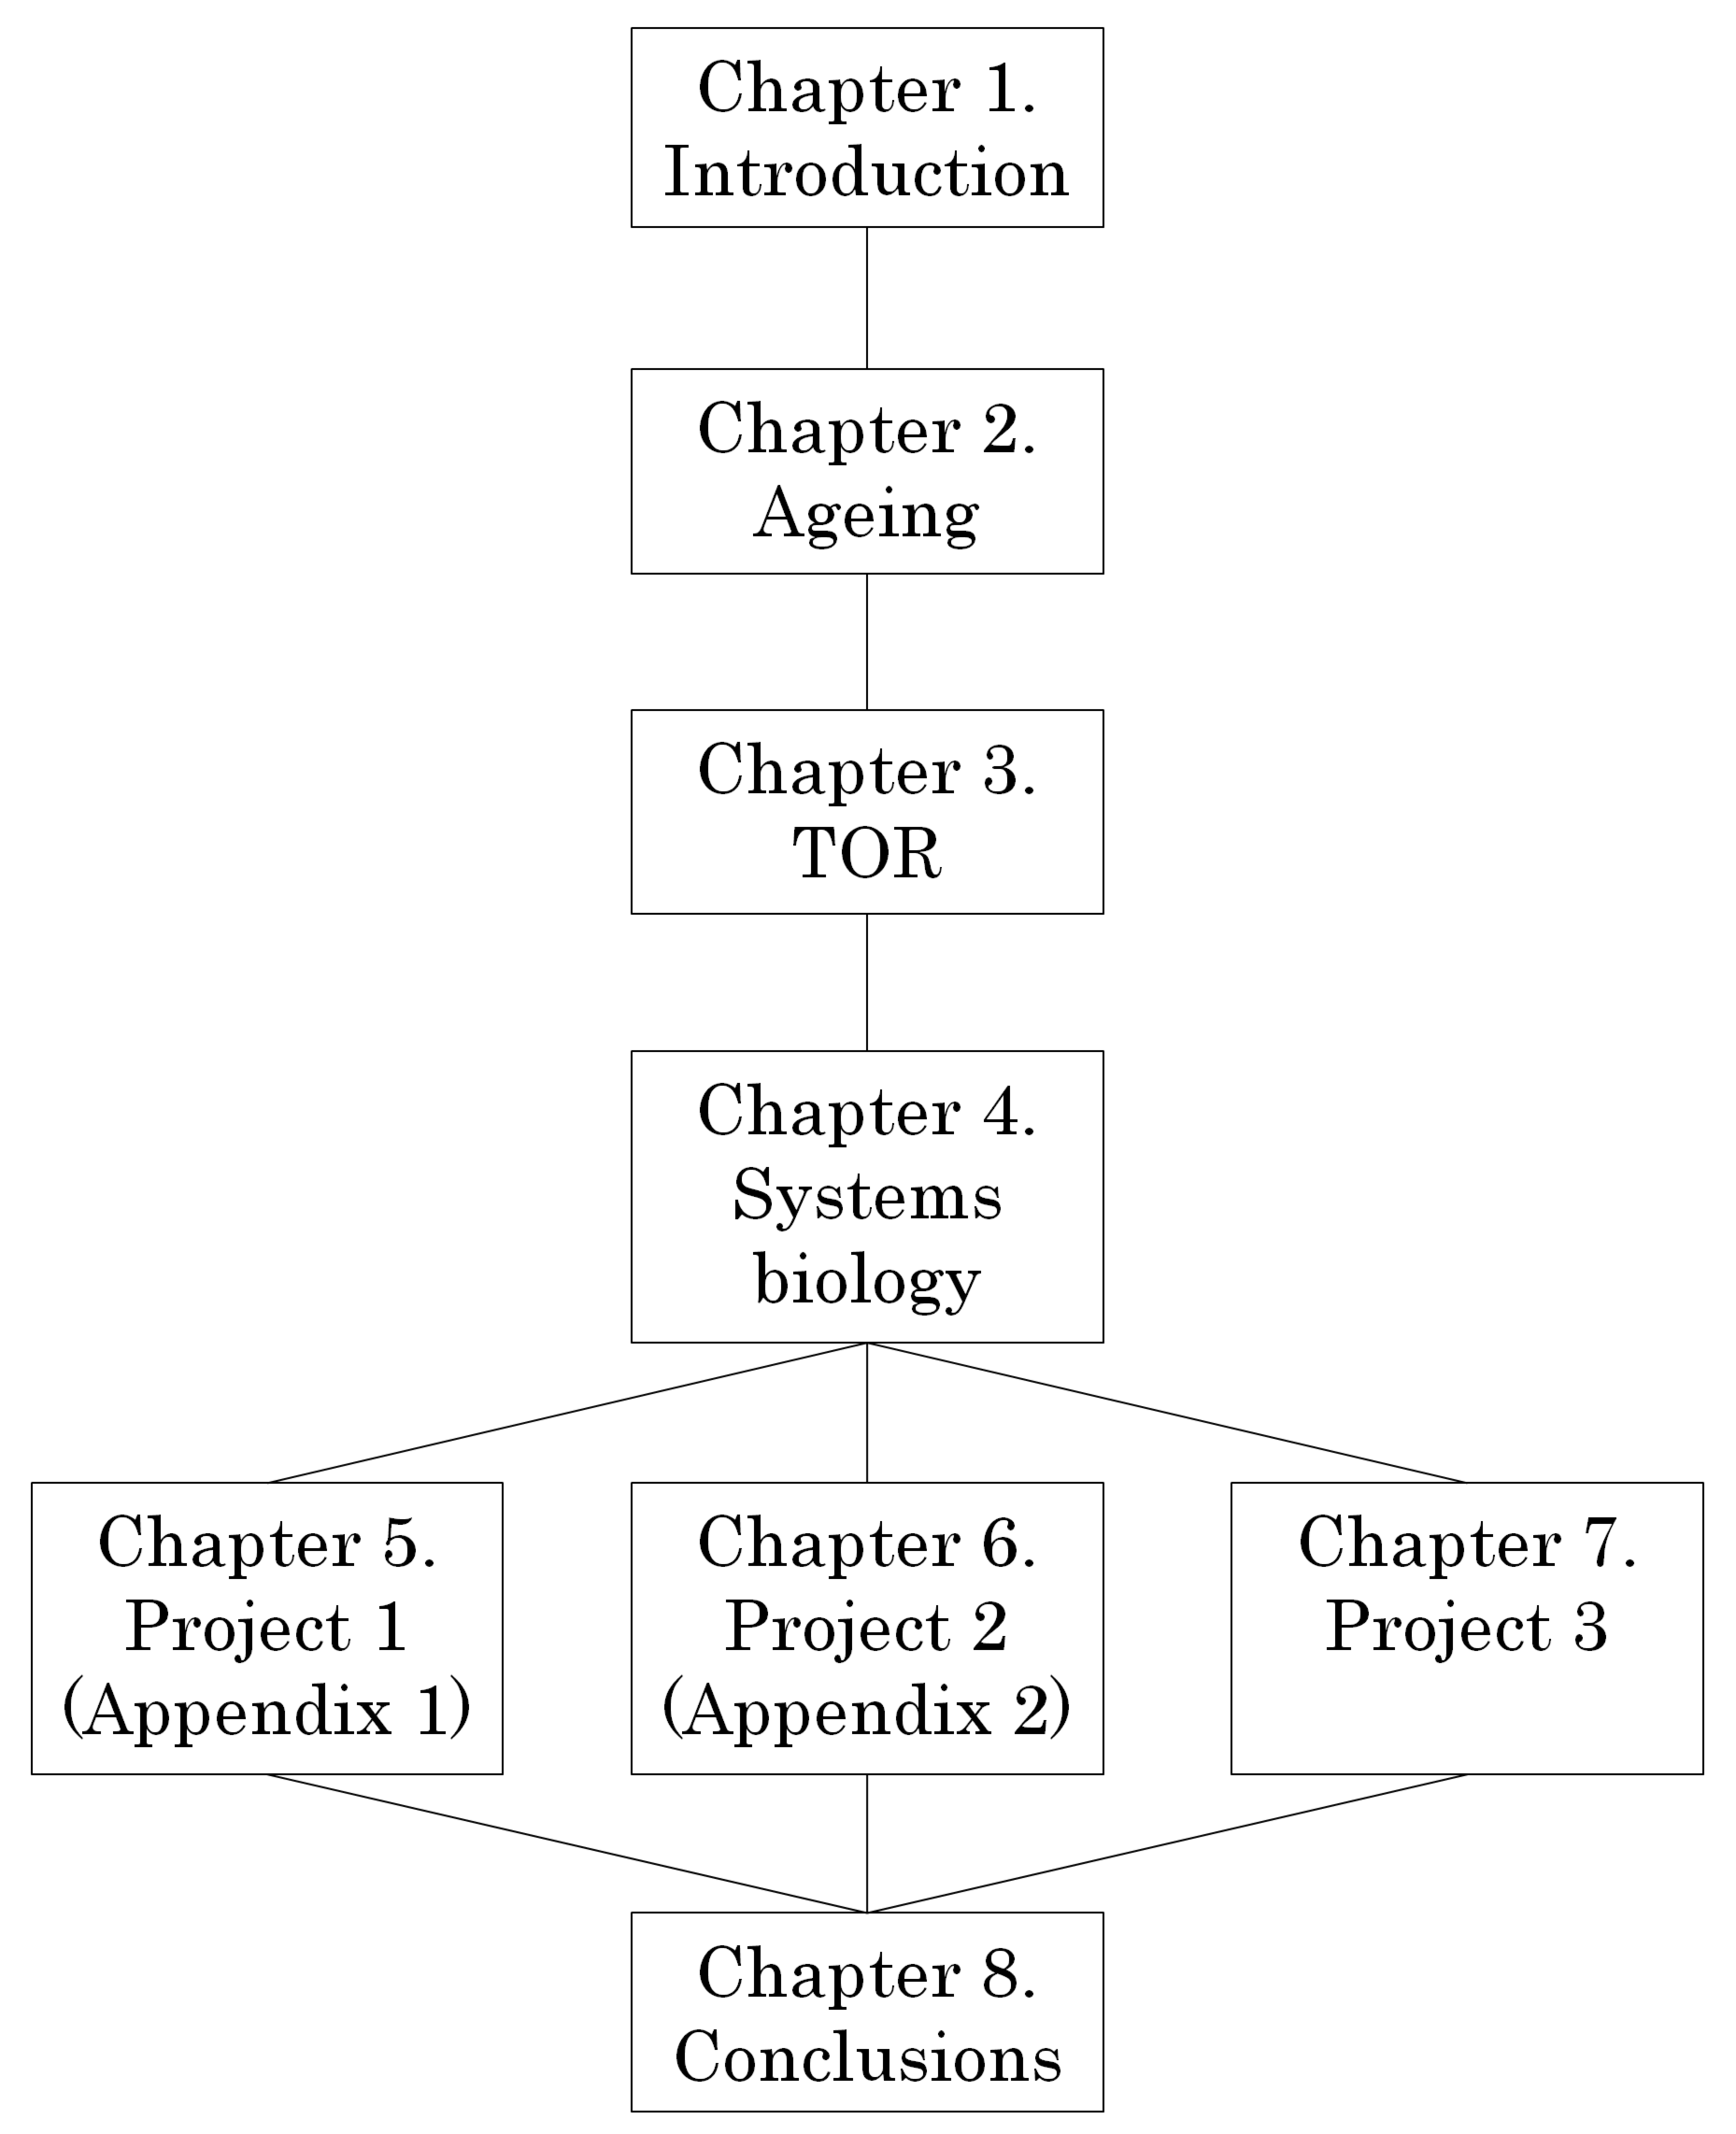
\includegraphics[width=5.0in]{outline.png}
		\caption[Thesis structure]{Thesis structure.}
		\label{fig:outline}
	\end{center}
\end{figure}
\clearpage





%%% ----------------------------------------------------------------------


%%% Local Variables: 
%%% mode: latex
%%% TeX-master: "../thesis"
%%% End: 

\graphicspath{{Chapter2/Chapter2Figs/}}

\chapter{TOR in ageing and age-related diseases}
\label{chap:TOR in ageing and age-related diseases}
The process of ageing and its role in disease has intrigued mankind for centuries. Despite this, a clear understanding of why and how ageing occurs is still far from being achieved. Among the proposed ageing theories, the disposable soma theory is one of the most comprehensive, widely applicable and well established. In this theory the problem of allocating resources to remove or repair molecular damage is central. One of the key systems that responds to resource availability is the nutrient sensing network. This network is a widely conserved intracellular system that serves to detect nutrient availability and govern an appropriate cellular response. Many studies have shown that inhibition of this network by nutritional, pharmacological and genetic intervention extends lifespan in a wide range of organisms including yeast, worms, flies and rodents. Of particular interest is the finding that Rapamycin, which inhibits a key component of the nutrient sensing network, suitably named the target of Rapamycin (TOR),
 is effective in extending lifespan in a similar range of organisms. Rapamycin was originally discovered in Easter island and shown to inhibit growth and proliferation within the cell, and is widely used to prevent organ transplantation rejection. It is an established drug and as a candidate for pharmacological intervention aimed at prolonging lifespan and healthspan, and reducing the impact of age-related diseases.\\
This chapter presents a summary on the biology of ageing and age-related diseases with particular emphasis on TOR.


\section{Theoretical foundations on ageing}
\label{sec:Theoretical foundations on ageing}
This section introduces the theoretical foundations of this study through a \emph{top-down} approach. Firstly, the disposable soma theory and the resource allocation problem are introduced. Secondly, the connection between this evolutionary theory of ageing and TOR-dependent cellular regulation is proposed.

\subsection{The disposable soma theory}
\label{subsec:The disposable soma theory}
Ageing is a progressive loss of function accompanied by increasing mortality and decreasing fertility with age. The disposable soma theory \citep{Kirkwood1977, Kirkwood1981, Kirkwood1991, FinchKirkwood_book2000, Shanley2000} considers the problem an organism faces in partitioning limited resources acquired from the environment between the physiological functions of maintenance/repair and reproduction. Investment in maintenance/repair will slow the rate of ageing whereas investment in reproduction is essential for producing offspring. The optimal decision that maximises Darwinian fitness will depend on the amount of resources available and on the environmental conditions but in general investment in maintenance/repair is inevitably less than required for indefinite survival and the accumulation of damage results in ageing. In the wild, life is constantly compromised by multiple extrinsic factors such as predators, food deprivation and temperature variability. In an unprotected environment, the risk of 
mortality is therefore high (see Figure \ref{fig:dst_resalloc_tor}A). Moreover, an organism is continuously challenged by internal damage, for instance due to injury, infections, diseases, malnutrition, toxins, oxidative stress, which must be repaired. Maintainance is crucial in order to preserve the soma in good enough condition for survival to ensure opportunities to reproduce. The physiological functions of repair and maintenance require a considerable amount of energy which has to be carefully allocated in the organism. This investment is compromised by the competing energy demand for reproduction which includes maintenance of the germline cells. As a consequence, the organism gradually degrades over time, becoming more susceptible to extrinsic and intrinsic risk factors, and ultimately dies.

\subsection{The resource allocation problem}
\label{subsec:The resource allocation problem}
In the disposable soma theory, resource allocation is the key problem as resources are limited and maintenance is costly. In an organism, these resources are allocated among the physiological functions of growth, maintenance and repair, storage and reproduction \citep{Kirkwood2008} (see Figure \ref{fig:dst_resalloc_tor}B). At the level of the organism, resource allocation is partially regulated by growth factors and nutrients, as variability in these two players significatively affects size and reproduction in \emph{Caenorhabditis elegans}, \emph{Drosophila melanogaster} and mice \citep{Holzenberger2001, Walker2005, Bass2007, Kapahi2009, Selman2009}. Similarly, at the level of the cell, resource allocation is regulated by growth factors, amino acids and energy \citep{Sengupta2010, Zoncu2011, Russell2011, Laplante2012}. In the cell, a key protein responsible for orchestrating resource allocation is the target of Rapamycin (TOR). Through resource availability, recognised by the cell as growth factors, 
nutrients and 
energy, TOR promotes cellular growth and proliferation, improves mitochondrial function increasing the amount of cellular energy, and inhibits conservative or recycling processes such as cell cycle arrest or autophagy \citep{Dunlop2009aa, Inoki2006aa, Stanfel2009, Yang2007aa, Kapahi2009} (see Figure \ref{fig:dst_resalloc_tor}C). Therefore, understanding the regulation of TOR and its interacting partners represent a crucial step in furthering our knowledge of ageing and uncovering potential therapies for extending healthspan and lifespan. 

\subsection{Links between TOR, mitochondria and ROS}
\label{subsec:Links between TOR, mitochondria and ROS}
In response to growth factors and nutrients TOR regulates protein translation and mitochondrial function \citep{Finley2009, Kaeberlein2007, Stanfel2009, Kaeberlein2010}. TOR can affect mitochondria in multiple ways. TOR can directly inhibit mitochondrial autophagy (mitophagy) impeding the degradation of dysfunctional mitochondria \citep{Lee2012}. Conversely, TOR also regulates global mitochondrial function through mitochondrial biogenesis \citep{Hock2009}. \\
There is substantial evidence on the link between mitochondria and reactive oxygen species (ROS). The majority of cellular ROS are generated as a by-product of ATP production by the mitochondrial electric transport chain (ETC) during oxidative phosphorylation \citep{Murphy2009}. The ETC activity can be measured by the mitochondrial membrane potential (see Figure \ref{fig:Tsutsui09_fig1_adapted}). Interestingly, ROS are responsible for the damage of mitochondrial DNA (mtDNA) subunits \citep{Shokolenko2009} which would lead to a gradual dysfunction of the mitochondria ETC mechanism \citep{Turrens2003}. Mitochondrial function would therefore enter a sub-optimal state characterised by low energy production (ATP) and high ROS generation. The establishment of this \emph{vicious cycle} between ROS production and mitochondrial ETC activity may lead to catastrophic dynamical changes inside a cell \citep{Turrens2003}.\\
From this prospective, it is clear that the insulin/TOR signalling regulation of mitochondrial function is essential to understand in order to selectively intervene for improving cellular functions and health.


\section{TOR-dependent interventions for extending lifespan}
\label{sec:TOR-dependent interventions for extending lifespan}
This section discusses two of the most well-known interventions for increasing lifespan in a TOR-dependent manner: caloric restriction and selective perturbation of TOR-dependent downstream partners.

\subsection{Caloric restriction}
\label{subsec:Caloric restriction}
Caloric Restriction (CR), defined as a reduction in calories without malnutrition, is the most well known nutritional intervention that leads to lifespan extension and prevention from various chronic diseases in protected environments \citep{Gredilla2005, Kapahi2010}. Although most studies report a positive effect for CR there are notable exceptions. In fact, CR was not found to extend lifespan or reduce the incidence of cancer in wild mice \citep{Harper2006} or rhesus monkeys \citep{Mattison2012}. Mutations in the insulin and insulin-like signalling pathway were the first genetic interventions confirmed to extend life in animals \citep{Kenyon2010}. Both insulin signalling and amino acids activate TOR, and reduced TOR activity increases lifespan \citep{Evans2010, Kapahi2004, Kaeberlein2009, Laplante2012}. In yeast, both replicative\footnote{Replicative lifespan counts the number of daughter cells generated by a mother cell prior to senescence \citep{Mortimer1959}.} and chronological\footnote{Chronological 
lifespan measures the amount of time a cell can survive within the G0 phase (quiescence) of the cell cycle \citep{MacLean2001}.} lifespans increase when TOR1 and TOR2 genes are deleted or pharmacologically inhibited. In general, reduced TORC1 activity has been demonstrated to increase lifespan in several organisms including single-celled budding yeast \emph{Saccharomyces cervisiae} \citep{Wanke2008}, invertebrate nematode \emph{Caenorhabditis elegans} and fruit fly \emph{Drosophila melanogaster} \citep{Kapahi2009}, mice \citep{Anisimov2010, Harrison2009} and rhesus monkeys \citep{Colman2009}. The effects of CR in the mTOR pathway are a progressive reduction of the IGF/PI3K/Akt/mTOR signalling, and an increase in AMPK \citep{Jiang2008}. This results in an enhancement of autophagy activity which could therefore limit the progression of age-related diseases and promoting lifespan \citep{Ravikumar2010}.



\subsection{Intervention on TOR downstream targets}
\label{subsec:Intervention on TOR downstream targets}
Another way to extend lifespan is by the regulation of TOR downstream targets or substrates, such as p70 ribosomal S6 kinase 1 (p70-S6K1) \citep{Selman2009} and 4E-binding protein 1 (4E-BP1) \citep{Kapahi2009}. These substrates promote the production of ribosomal proteins and ribosome biogenesis and a reduced production is associated with increased lifespan. In addition to the regulation of mRNA translation, ageing is also modulated by autophagy \citep{Cuervo2008, Blagosklonny2009, Hansen2008, Blagosklonny2010}. A reduction in TOR activity obtained by Rapamycin-induced inhibition or CR, stimulates the autophagy process. Through autophagy \citep{Alvers2009}, non-vital and damaged components are destroyed and transformed into nutrients, extending lifespan. It is worth noting that, in contrast to yeast, in mammals TOR can be regulated in different ways in different tissues and thus, it is also important to understand the consequences of TOR inhibition within a specific tissue. In fact, inhibition of TORC1 may 
be beneficial in some tissues, but in contrast, may be detrimental to others \citep{Russell2011}.


\section{TOR in age-related diseases}
\label{sec:TOR in age-related diseases}
In this section, the role of TOR in the most significant age-related diseases is outlined to provide an overview on the impact that TOR research could have on society by increasing both lifespan and healthspan.

\subsection{Cancer}
\label{subsec:Cancer}
Mutations of important cell check-point proteins, such as the tumour suppressor PTEN or the oncogene protein Akt/PKB, as well as an elevated mTOR activity, are often discovered in many cancers. The interest of cancer research in mTOR is also related to the effects of the natural drug Rapamycin \citep{Bjornsti2004}, which has been shown to extend lifespan in cancer-prone mice \citep{Anisimov2010}. Following Rapamycin treatment, cells tend to arrest their life-cycle at G1 phase because of insufficient cell growth input \citep{Bjornsti2004}. A pure Rapamycin treatment in cancer does not provide significant improvements because the drug only partially inhibits mTORC1 and does not affect mTORC2 \citep{Janes2010}. However, the adoption of radiotherapy or chemotherapy drugs administered in combination with Rapamycin has been shown to be more effective in cancer treatment \citep{Rosner2008}. Due to the limitation of Rapamycin, interest has increased in the study of cancer treatments by more specific TOR inhibitors, 
such as Torin and PP242 \citep{Janes2010, Liu2011, Feldman2009, Laplante2012}. mTOR is also responsible for the activation of the Vascular Endothelial Growth Factor (VEGF), a signalling pathway related to vasculogenesis, process in which new blood vessels are created, and angiogenesis, which is the growth of blood vessels from existing ones \citep{Treins2002}. This stimulation is essential for cancer maintenance and development of metastasis.

\subsection{Diabetes and Obesity}
\label{subsec:Diabetes and Obesity}
Diabetes is a serious age-related disease and is affected by age-related increase in obesity. There are two forms of diabetes, Type 1 and Type 2, and both involve the mTOR signalling pathway. In the former, the destruction of pancreatic $\beta$-cells leads to insufficient insulin production. As a consequence, glucose levels increase in blood and urine and patients need repeated administration of insulin, typically by injection \citep{Lehuen2010}. Type 2 diabetes is mostly connected to caloric excess and lack of physical activities, which are both associated with the elderly. Type 2 diabetes is associated with over activation of the mTOR pathway and the consequent insulin resistance and deficiency. One feature is an upregulation of mTOR due to amino acids which leads to a sustained p70-S6K-dependent negative feedback activation and consequent constitutive degradation of insulin receptor substrate (IRS1) \citep{Dann2007, Tremblay2007, Laplante2012} (see Figure \ref{fig:mTOR} for a conceptual map of the TOR 
network). Conversely, inhibition of mTORC1 activity with Rapamycin reduces the p70-S6K activity restoring the normal sensitivity of the IRS1/PI3K/Akt pathway. Type II diabetes is usually linked to obesity and TOR is also an important regulator of lipid synthesis \citep{Rosner2008, Laplante2012}. In hepatic cells mTOR exerts a role in the lipogenic gene expression by regulating the transcription factor sterol regulatory element binding protein 1c (SREBP-1c) \citep{Peterson2011}. Amino acids represent a key regulator of both mTORC1 and SREBP-1c. Recently, SREBP-1c has been found to be activated by protein kinase C $\beta$ (PKC$\beta$) \citep{Yamamoto2010}, which is stabilised and phosphorylated by mTORC2 \citep{Ikenoue2008}. Therefore, a long-term continuous activity of mTORC1 and mTORC2 can determine insulin resistance and hepatic steatosis through IRS1 degradation and SREBP-1c activation.

\subsection{Neurodegeneration}
\label{subsec:Neurodegeneration}
The mechanisms by which neurons lose their functionality are not yet completely understood. Interestingly, CR and inhibition of mTOR signalling have been proposed as possible candidates in order to protect neurons and reduce neuronal loss during ageing by promoting autophagy. These effects could limit and also reduce damage causing neurological disorders such as Alzheimer's, Parkinson's, Huntington's, Creutzfeldt-Jakob's and dementia diseases \citep{Rosner2008}. These neurodegenerative diseases are characterised by an accumulation of aggregated mutant proteins in the intracellular space. For example, Huntington's disease presents polyglutamine (polyQ) expansion repeats; mutant forms of $\tau$, a protein thought to contribute to neurofibrillary tangles, are discovered in Alzheimer's disease; whereas $\alpha$-synuclein and $\beta$-amyloid mutants accumulate Parkinson's disease \citep{Levine2008, Glick2010}. Autophagy can potentially benefit these diseases by removing these aggregates. Rapamycin or Metformin 
treatment could be used to inhibit mTORC1 signalling and increase autophagy levels \citep{Hara2006, Komatsu2006}. The role of autophagy in neurodegenerative diseases is also highlighted by the fact that, mice with deficiency of autophagy-related 5/7 proteins (Atg5, Atg7) increased the accumulation of mutant proteins in neurodegenerative diseases \citep{Hara2006, Komatsu2006}. Finally, other important neuropsychiatric disorders, such as autism, epilepsy and mental retardation, are often linked to mutations of TSC genes, upstream of mTORC1 \citep{Gomez1999, Tee2002}. Thus, an inhibition of mTOR may improve the impact of these diseases in affected patients.

\subsection{Hamartoma syndromes}
\label{subsec:Hamartoma syndromes}
The Hamartoma syndromes represent genetic diseases characterised by benign tumours which grow in brain and various organs such as lungs, kidneys, skin and heart. Hamartoma syndromes include: tuberous sclerosis complex syndrome (TSCS), Cowden syndrome (CS) and Peutz-Jeghers syndrome (PJS) \citep{Inoki2005}. TSC syndrome is due to a mutation of either TSC1 or TSC2 which disrupts TSCs complex hyperactivating mTORC1. This hyperactive mTORC1 promotes cell over-growth and tumour formation in TSC patients \citep{Umeoka2008}. In CS patients, a mutated PTEN leaves activated PIP3 hyperstimulating mTORC1. As a consequence, PIP3 hyperactivates Akt/mTORC1 causing a dysregulation of cellular growth and proliferation \citep{Pilarski2009}. A similar effect can be observed in PJS patients, due to a mutation of the protein LKB1 \citep{Beggs2010}. A mutation of LKB1 prevents the formation of AMPK and leaves activated mTORC1 even though in hypoxia conditions \citep{Krymskaya2009}. Cells induced by a hyperactive mTORC1 grow 
larger, faster and with different structure than normal cells, increasing susceptibility to tumourigenesis. Rapamycin can be used for reducing tumour size by inhibiting mTORC1. To reduce the risk of malignancy progression, it is also important to restrict the activity of the PI3K/Akt pathway directly by using PI3K inhibitor drugs, such as LY294002 or Wortmannin. Due to the crucial role of mTORC2 in the phosphorylation of Akt, new TOR specific inhibitors could improve the treatment of the Hamartoma syndromes.


\section{Figures}
\label{chap2:Figures}

\clearpage
%\vspace{2cm}

\begin{figure}[tb]
%\begin{figure}[h]
	\begin{center}
		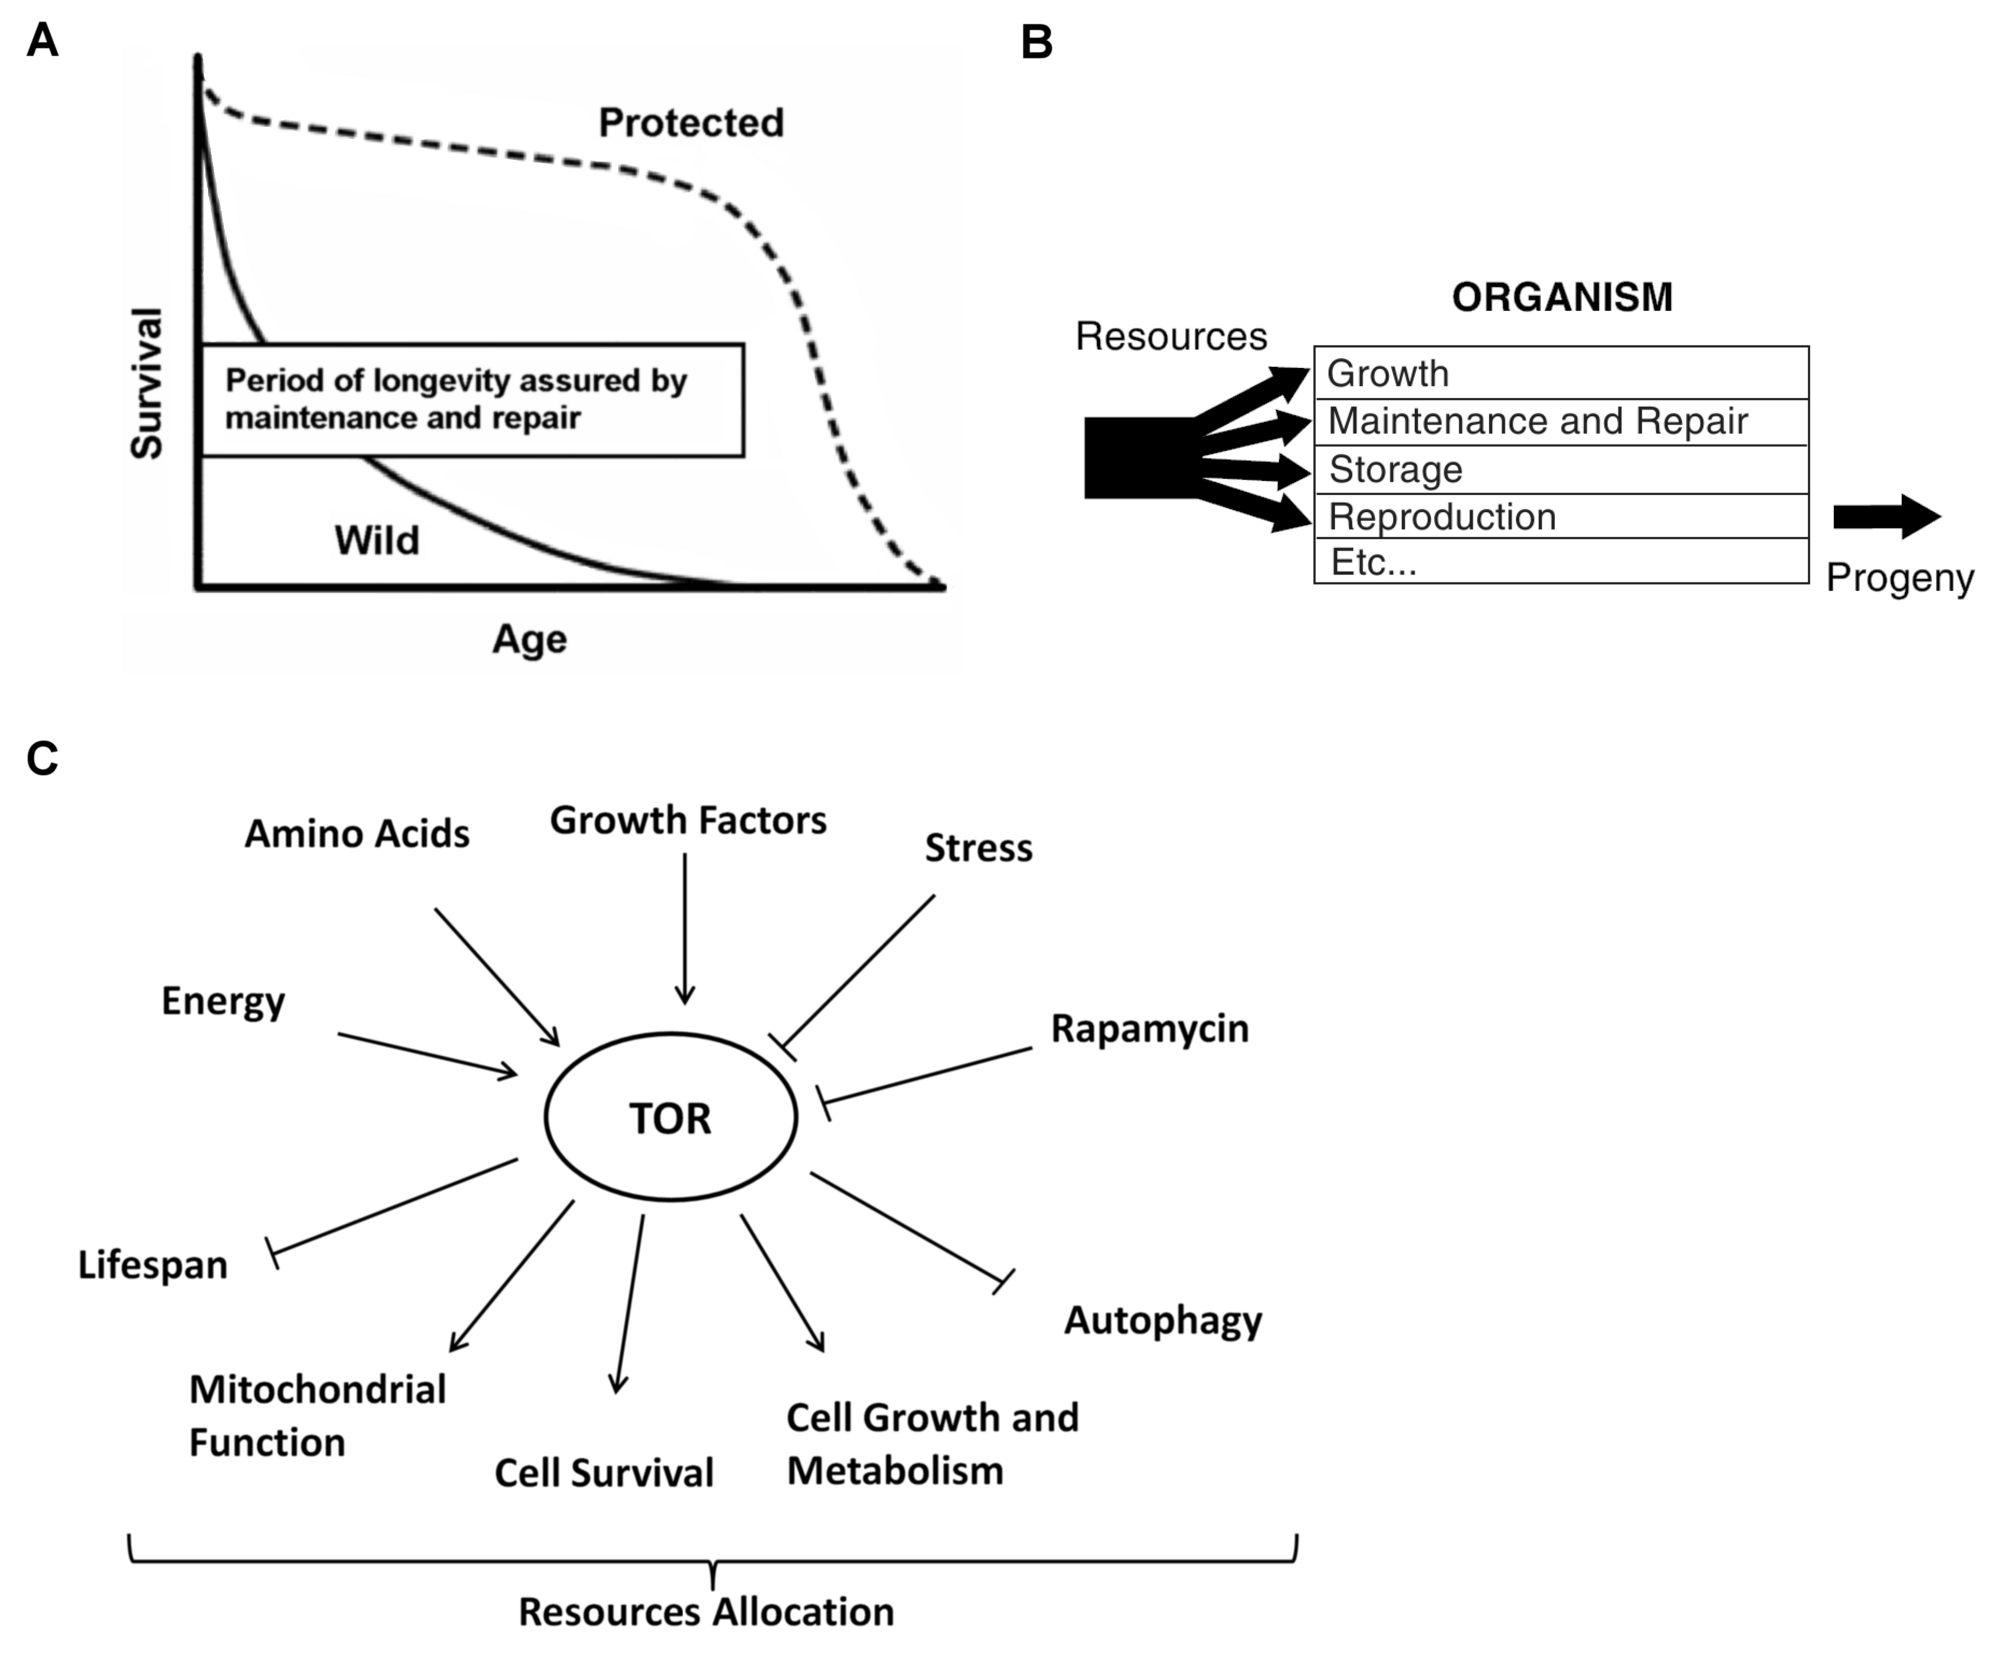
\includegraphics[width=5.6in]{dst_resalloc_tor.png}
		\caption[Disposable soma theory, resource allocation and TOR]{Disposable soma theory, resource allocation and TOR. (A) Lifespan differences between wild and protected environments. Adapted from \citep[Fig. 1]{Kirkwood2008}. (B) Resources allocation in the disposable soma theory of ageing \citep{Kirkwood1977, Kirkwood1981,Kirkwood2008}. In this theory, the problem of resource allocation is crucial since resources are limited and maintenance is costly. Adapted from \citep[Fig. 3]{Kirkwood2008}. (C) TOR in ageing. In response to stimuli such as insulin or growth factors, amino acids, energy and stress, Target of Rapamycin (TOR) kinase governs numerous age-related cellular processes regulating the allocation of resources.}
		\label{fig:dst_resalloc_tor}
	\end{center}
\end{figure}

\clearpage

\begin{figure}[tb]
	\begin{center}
		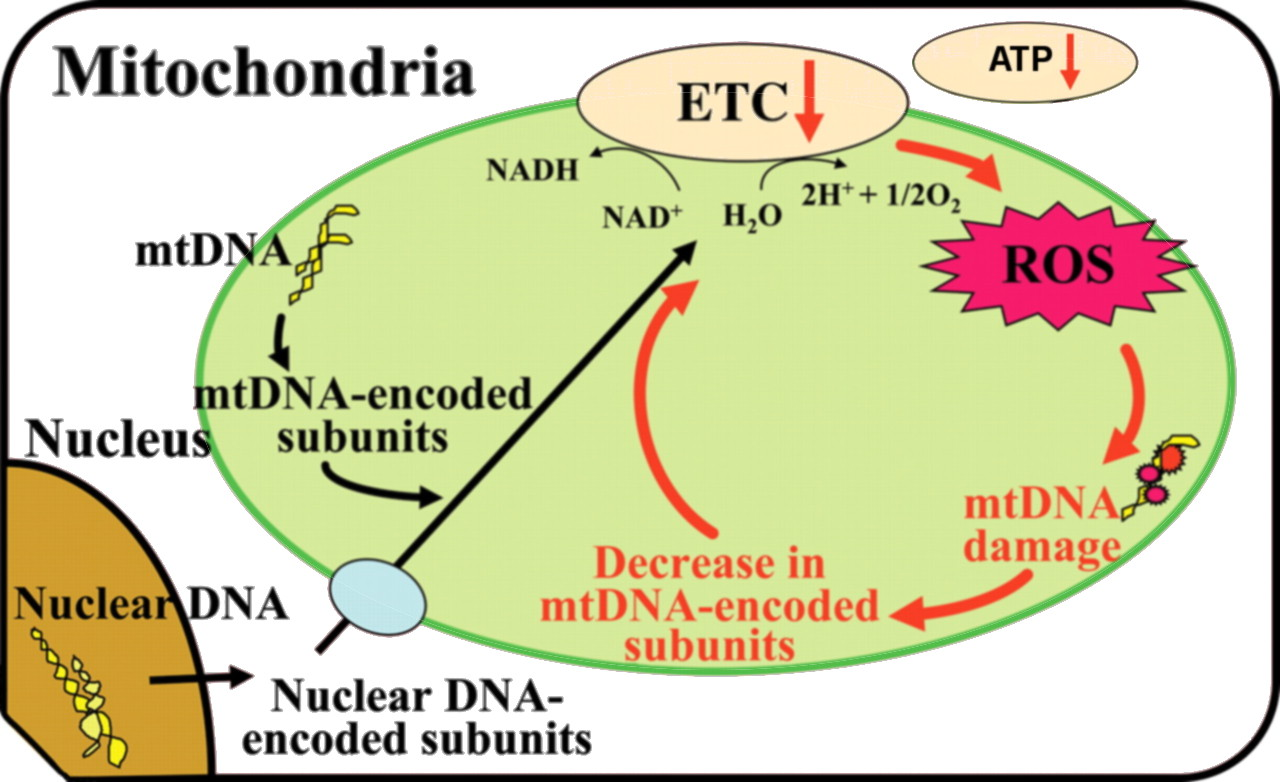
\includegraphics[width=3in]{Tsutsui09_fig1_adapted.jpg}
		\caption[ROS production and mitochondrial dysfunction]{ROS production and mitochondrial dysfunction. Mitochondrial DNA (mtDNA) in combination with nuclear DNA encode proteins building the mitochondrial electron transport chain (ETC), whose activity can be measured by mitochondrial membrane potential. Through ETC, molecules of adenosine triphosphate (ATP) are synthesised and utilised by the cell as an energy supply. Aside from ATP production, mitochondrial ETC also produces reactive oxygen species (ROS) as a waste product. ROS accumulation, due to a lack of ROS detoxification, severely damages mtDNA subunits, establishing a vicious circle which decreases mitochondrial function, energy levels within the cell, and increases ROS production and mutated mtDNA. Adapted from \citep[Fig. 1]{Tsutsui2009}.}
		\label{fig:Tsutsui09_fig1_adapted}
	\end{center}
\end{figure}

\clearpage




% ------------------------------------------------------------------------


%%% Local Variables: 
%%% mode: latex
%%% TeX-master: "../thesis"
%%% End: 

\graphicspath{{Chapter3/Chapter3Figs/}}


\chapter{mTOR network: an overview}
\label{chap:mTOR network: an overview}
TOR kinase is centrally located in a complex signalling network that responds to the availability of cellular resources. TOR is positively regulated by growth factors, nutrients and energy uptake. Through these signals, the kinase activates protein translation initiation and elongation mechanisms, regulates cell growth and metabolism, improves mitochondria function and transmits signals for cell survival. TOR-activated downstream targets inhibit apoptosis, autophagy and cell cycle arrest. Conversely, nutritional or energetic stress conditions negatively control TOR activity. The TOR network is further complicated by several feedback mechanisms that work at different time-scales and hamper a full understanding. This chapter presents details of TOR kinase and the two protein complexes containing TOR in mammals (mTOR) to place TOR in the network of related upstream and downstream signals.

\section{mTOR, Rapamycin and AGC kinases}
\label{sec:mTOR, Rapamycin and AGC kinases}
This section introduces the mammalian TOR kinase from a biochemical point of view and the first natural drug found to partially inhibit the kinase. A short introduction of the mTOR-dependent AGC kinases is also presented as useful background to understanding the complexity of mTOR network.

\subsection{mTOR: kinase and complexes}
\label{subsec:mTOR: kinase and complexes}
The protein TOR was discovered in the early 1990s in genetic screens in yeast for the resistance to Rapamycin \citep{Heitman1991}. TOR1 and TOR2 in yeast and the single mammalian homolog mTOR which are present in two multi-protein complexes, mTORC1 and mTORC2, integrate upstream signals to regulate several downstream processes.\\
The mammalian TOR, mTOR, is a serine/threonine protein kinase which belongs to the phosphatidylinositol kinase (PIKK) family in which the catalytic domain presents significant homology to that of other phosphoinositide 3-kinases (PI3Ks) although mTOR has protein rather that lipid targets. The protein mTOR is composed of five important components. From its N-terminus: a tandem HEAT domain involved in substrate binding; a FAT domain whose function is currently unknown; an FRB domain which provides a docking site for the ligand FKBP12; finally, there are the fundamental mTOR kinase domain and the FATC (FAT C-terminus) domain \citep{Wullschleger2006, Hay2004}. The details of the FATC domain activity are still unknown.\\
The mTOR kinase represents a central regulator of eukaryotic growth and cell division when stimulated by nutrients and growth factors, energy signals and cellular stresses. mTOR was found to exist in two complexes named mTOR Complex 1 (mTORC1) and mTOR Complex 2 (mTORC2) which are structurally and functionally different (see Figure \ref{fig:mtor_complexes}).\\
Whenever stimulated by amino acids and growth factors such as insulin, mTORC1 controls multiple cellular processes such as autophagy inhibition, mRNA translation, ribosome biogenesis, lipid storage and cell cycle progression. mTORC2 responds only to growth factors and serves to regulate actin polymerisation and promotes the phosphorylations of Akt/PKB and serum- and glucocorticoid-inducible kinase 1 (SGK1). In contrast to mTORC1, the role and the interactions of mTORC2 within the cell still remains mostly unknown. 

\subsection{The natural drug Rapamycin}
\label{subsec:The natural drug Rapamycin}
Rapamycin was discovered in Easter Island and is an immunosuppressant drug used to prevent organ rejection in transplants \citep{Saunders2001}. It is the first drug to have been shown to extend lifespan in a mammal \citep{Harrison2009}. Also, it has been shown to have significant anti-proliferative properties which made it an interesting drug candidate in cancer research \citep{Rao2004, Vignot2005}.\\
Rapamycin binds with a protein named FK506-binding protein 12 kDa (FKBP12) \citep{Choi1996} which associates directly with TOR, altering its normal kinase activity, ultimately resulting in cell growth arrest \citep{Evans2010}. When bound to the FRB domain of mTOR by FKBP12 protein, Rapamycin blocks some of the physiological functions of mTOR by inhibiting part of the mTOR autophosphorylation. This intrinsic mTOR activity is fundamental for mTOR to modulate signals to its substrates. Interestingly, the activity of both mTOR and Rapamycin are highly preserved among eukaryotes. Of particular interest in ageing is the fundamental role of TOR in the regulation of autophagy, a key process responsible for the degradation of cytosolic components.

\subsection{mTOR-dependent regulation of AGC kinases}
\label{subsec:mTOR-dependent regulation of AGC kinases}
The mTOR network contains several important kinases belonging to the AGC family of approximately 60 kinases. In the context of the mTOR network, the most important AGC kinases are PDK1, Akt/PKB \citep{Alessi2004, Alessi2004b}, p70 ribosomal S6 kinase (p70-S6K) \citep{Volarevic2001}, p90 ribosomal S6 kinase (RSK) \citep{williams2000}, serum- and glucocorticoid- inducible kinase (SGK1) \citep{Jacinto2008} and protein kinase C (PKC) \citep{Newton2003}. AGC kinases are characterised by three important phosphorylation sites, whose activation provides differential functionality. A partial activation of the kinase is achieved by phosphorylation at the activation loop, also called T-loop, in the kinase domain. This phosphorylation enables conformational change in the protein structure which exposes the kinase hydrophobic motif (HM), located in a C-terminal tail region, on the protein surface. Phosphorylation at this region determines a full activation of the AGC kinase and further functionality \citep{Pearce2010}. 
The third and least characterised phosphorylation site or region is the turn motif phosphate which is also located in the protein tail. Its function is to stabilise the phosphorylation of the kinase by sheltering the hydrophobic motif from dephosphorylation \citep{Hauge2007, Pearce2010}.\\

\section{Upstream signalling pathways of mTOR}
\label{sec:Upstream signalling pathways of mTOR}
Multiple signalling pathways have a regulatory influence on the mTOR Complexes 1 and 2. This section presents the four major inputs of mTOR: growth factors, amino acids, energy and hypoxia. The most important cross-talks from these signals to other pathways are also mentioned.

\subsection{The insulin insulin-like signalling pathway}
\label{subsec:The insulin insulin-like signalling pathway}
Insulin and insulin-like signalling (IIS) is mediated at the cell membrane by a specific insulin receptor (IR). In the presence of insulin molecules on the external membrane surface, the insulin receptor is auto-phosphorylated at several tyrosine residues transmitting the signal in the internal membrane surface. Among several proteins activated by IR, the insulin receptor substrate (IRS) is crucial in the IIS pathway. The IRS binds with phosphoinositide 3-kinase (PI3K) forming a complex which enables the production of  phosphatidylinositol (3,4,5)-trisphosphate (PI(3,4,5)P3) from phosphatidylinositol (4,5)-bisphosphate (PI(4,5)P2) or phosphatidylinositol (3,4)-bisphosphate (PI(3,4)P2) through phosphorylation at the membrane surface \citep{Polak2009}. The activity of PtdIns(3,4,5)P3 is negatively controlled by phosphatase and tensin homolog (PTEN) and SH2-containing inositol phosphatase (SHIP), which convert the PI(3,4,5)P3 in the form of PI(4,5)P2 and PI(3,4)P2 respectively. Upon insulin or insulin-like 
stimuli, phosphoinositide-dependent kinase-1 (PDK1) and Akt, also known as Protein Kinase B (PKB), relocalise from the cytoplasm to the membrane surface and their Pleckstrin Homology (PH) domain binds with PI(3,4,5)P3 molecules \citep{Polak2009}. This binding exerts a conformational change in Akt/PKB which is necessary to enable PDK1 to phosphorylate Akt at T308 at the T-loop \citep{Kobayashi2008, Alessi2004b, Kobayashi1999, Alessi2008, Alessi2004, Toker2000, Biondi2004}. Once phosphorylated at T308, Akt affects the integrity of the tuberous sclerosis complex (TSC1/TSC2) by phosphorylating TSC2 at S924 and T1518 \citep{Inoki2002, Potter2002}. Whereas TSC1 mainly serves for the stabilisation of the TSC1/TSC2 complex, TSC2 presents a GAPase Activating Protein (GAP) domain which controls GTPase activity of mTORC1 activator Ras-homolog enriched in brain (Rheb). Therefore, TSC2 switches off Rheb by hydrolysing Rheb activator guanosine-5'-triphosphate (GTP) to guanosine diphosphate (GDP), whereas guanine 
nucleotide-exchange factors (GEFs) reverse this reaction by freeing GDP molecules from the GTPase and thus promoting GTP formation and consequent GTP-bound Rheb activation. Whenever TSC1/TSC2 complex is disrupted, GTP-bound Rheb is free to bind with mTOR Complex 1 (mTORC1) at the lysosomal surface, mediating the insulin signalling \citep{Huang2008review}. Regarding mTORC2, it is known that the complex is sensitive to growth factors, such as insulin, but little is known about how this activation happens. Insulin stimulation has been shown to be responsible for the phosphorylation of Rictor at T1135, even when Rictor is not associated with mTOR, as this phosphorylation was inhibited upon Wortmannin treatment \citep{Boulbes2010}. Recent studies have shown the presence of a positive feedback from TSC1/TSC2 to mTORC2, whereas a direct association between the dimer and mTORC1 is not known. These authors showed that the heterodimer could positively regulate mTORC2 in a Rheb-independent manner \citep{Huang2008, 
Rosner2008, Sparks2010}. These studies used Akt-S473 (see Section \ref{subsec:Akt-S473}), which is dependent on the p70-S6K-dependent negative feedback loop (see Section \ref{subsec:The downstream substrate p70-S6K}), as a marker of mTORC2, instead of a specific direct readout of mTORC2 activity. Although several speculations of mTORC2 activation have been proposed, a comprehensive study of the modalities of mTORC2 activation has yet to be conducted and this will be the subject presented in Section \ref{chap:A dynamical network model of mTOR signalling reveals TSC-independent mTORC2 regulation} (see Figure \ref{fig:mTOR}).

\subsection{The amino acids signalling pathway}
\label{subsec:The amino acids signalling pathway}
Amino acids such as Leucine, Tryptophan and Phenylalanine \citep{Taylor2002, Thedieck2009, Taylor2009} play a crucial role in regulating the mTOR network and mTORC1 activation, although surprisingly the mechanisms are still mostly unknown. Recent studies have revealed the presence of new Rag proteins which are necessary for the mTORC1 activation by amino acids \citep{Kim2008} (see Figure \ref{fig:mTOR}). Rag proteins are a family of four small GTPases, RagA, RagB, RagC and RagD, belonging to the Ras family. Rags associate as heterodimers formed by RagA or RagB, with RagC or RagD \citep{Kim2008, Sancak2008}. mTORC1 and Rags associate in the presence of amino acids, in particular leucine. Rags do not directly activate mTORC1, but allow mTORC1 to bind with Rheb which is necessary for mTORC1 activation. Interestingly, a more recent study \citep{Sancak2010} based on mass spectrometry analysis, has discovered the presence of a complex named Ragulator. Whenever stimulated by amino acids, Ragulator is responsible 
for the mTORC1 translocation to the lysosomal surface and the subsequent association between mTORC1 and the heterodimer Rags. Once mTORC1 localises to the lysosomal surface, an insulin stimulation can enhance mTORC1 activation by promoting the binding between GTP-bound Rheb and mTORC1. This synchronised confluence of the insulin and amino acids signalling pathways on the lysosomal surface could explain why insulin/IGF stimulation without amino acids is not sufficient for the activation of mTORC1 \citep{Drummond2008, Sancak2010}. Conversely, in the absence of amino acids mTORC1 localises to the cytoplasm \citep{Kalender2010}. Therefore, amino acids are essential for activating Ragulator which transfers mTORC1 to the lysosomal compartment and binds it with its activator Rheb. \\
Little information is known about how amino acids regulate the Rag GTPase proteins. \citet{Duran2012_rags}, from the lab of Hall, recently focused on glutamine, an amino acid involved in cell growth and metabolised through glutaminolysis to produce $\alpha$-ketoglutarate. The authors reported that glutamine combined with leucine activated Rag GTPase complex and promoted lysosomal translocation and activation of mTORC1 by enhancing glutaminolysis and $\alpha$-ketoglutarate production. Another recent study showed that SH3 domain-binding protein 4 (SH3BP4) negatively regulates Rag GTPase complex by binding to the inactive form of the complex under amino acids starvation conditions. Once bound to SH3BP4, Rag GTPase complex is unable to switch state and therefore to interact with and activate mTORC1. This leads to an inhibition of mTORC1 activity in a Rag GTPase-dependent manner \citep{Kim2012_SH3BP4}.\\
Amino Acids were also shown to partially activate mTORC2 and its readout Akt-S473 indirectly via class I PI3K  \citep{Jacinto2004, Tato2011Amino} although the detail of this connection is still unclear.

\subsection{The energy signalling pathway}
\label{subsec:The energy signalling pathway}
Another important regulator of mTOR is the energy signalling pathway \citep{Thedieck2009}. The main component of this signalling cascade is Adenosine Monophosphate-activated Protein Kinase (AMPK). AMPK is a trimeric complex formed by $\alpha$, $\beta$ and $\gamma$ subunits, which are necessary to maintain protein stability and function. AMPK is directly regulated by the tumour suppressor Liver Kinase B1 (LKB1). LKB1 is activated under energy or nutrient stress conditions and acts as a growth and proliferation suppressor. In adipocyte cells, LKB1 is negatively regulated via the androgen receptor, whereas positively via oestrogen receptor alpha \citep{McInnes2012}. When in a complex with the proteins STRAD and MO25, active LKB1 phosphorylates the AMPK-$\alpha$ subunit activation loop under conditions of energy stress, and this is sufficient for AMPK activation \citep{Shackelford2009}. LKB1 is of clinical importance as it plays a key role in maintaining cell polarity and lack of LKB1 is associated with Peutz-
Jeghers syndrome and other forms of cancer. \\
AMPK is an energy level sensor. Whenever the number of AMP molecules is much greater than ATP, the cell is in a low-energy status. In response to energy stress, AMPK becomes active in order to maintain energy homoeostasis in cell metabolism. Under such energy-stress conditions, the $\gamma$ subunit of AMPK binds directly with AMP molecules and undergoes a conformational change, becoming activated. Once activated, AMPK phosphorylates the unit TSC2 of the TSC1/TSC2 complex at T1271 and S1387, increasing the dimer GTPase activity \citep{Inoki2003, Inoki2005}. In addition, active AMPK phosphorylates the mTORC1 scaffold protein Raptor at S722 and S792, inhibiting it \citep{Gwinn2008}. Therefore, AMPK negatively controls mTORC1 through TSC1/TSC2 up-regulation and Raptor inhibition (see Figure \ref{fig:mTOR}). 

\subsection{The hypoxic signalling pathway}
\label{subsec:The hypoxic signalling pathway}
Hypoxia, which is referred to as a condition of low levels of oxygen, plays a role in the TOR network. Activated mTORC1 promotes the transcription of Hypoxia-inducible factor 1 (HIF-1) heterodimeric complex (see Figure \ref{fig:mTOR}). HIF-1 is differentially regulated depending on hypoxic or normoxic conditions in the cell. Under hypoxic conditions HIF-$\alpha$ binds with HIF-$\beta$ and the dimer then migrates from the cytosol to the nucleus and induces transcription of genes required for cellular adaptive response to hypoxic stress \citep{Dery2005}, such as erythropoietin (EPO), p300 and POLII \citep{Maxwell2005}. HIF-1 also promotes glucose metabolism \citep{Huang2004, Ke2006} and angiogenesis by activating the Vascular Endothelial Growth Factor (VEGF) pathway \citep{Gray2005, Klimova2008}. Interestingly, HIF-1 activates the transcription of the two genes Redd1 and Redd2 which inhibit mTOR in a TSC1/TSC2-dependent manner \citep{McCarthy2004, Brugarolas2004}, thereby providing a negative feedback loop. \
citet{Brugarolas2004} showed that Redd1/2 is required for down-regulating mTORC1 by promoting TSC1/TSC2 activity in a hypoxia-dependent and energy-independent manner. The hypoxic signalling pathway through mTORC1 also involves the protein Bnip3 which has been shown to be enhanced by HIF-1$\alpha$ subunit, under hypoxia conditions \citep{Wouters2008}. Bnip3 inhibits the GTP form of Rheb, directly reducing mTORC1 activation. In addition, Bnip3 was demonstrated to positively regulate autophagy \citep{Bellot2009}. Instead, in case of normoxic conditions, HIF-1 is rapidly hydroxilated by EGLN1/PHD1 and EGLN2/PHD2 at several prolines. Once HIF-1 is hydroxilated, the interaction with Von Hippel-Lindau (VHL) is facilitated, increasing HIF-1 ubiquitination and proteasomal degradation \citep{Dery2005, Maxwell2005}. 

\subsection{Other signalling pathways}
\label{subsec:Other signalling pathways}
In addition to mTOR other kinases in the network have an important role. Among these, Akt and IRS are potentially the two most important examples. Akt plays a direct role in glucose metabolism by phosphorylating and inhibiting Glycogen Synthase Kinase 3 (GSK-3). GSK-3 phosphorylates and inhibits Glycogen Synthase (GS), which is involved in the synthesis of glycogen from glucose \citep{Embi1980}. Akt also controls other cellular processes, such as cell survival and proliferation. Through phosphorylation, Akt enhances the oncogene protein murine double minute 2 (MDM2), an E3 ubiquitin ligase and the main repressor of p53, and deactivates FoxO. By inhibiting FoxO and p53 activity, the apoptotic signalling cascade composed of Bim-Bcl-2-Bax is repressed, thereby favouring cell survival. Akt deactivates several genes, such as Wee1, p27Kip1, p21Cip, which are involved in cell cycle arrest. Through these inhibitions, Akt promotes cell proliferation.\\
IRS has multiple activity when stimulated by growth factors. Besides propagating the insulin signalling by binding with PI3K (see Section \ref{subsec:The insulin insulin-like signalling pathway}), IRS binds to Growth factor receptor-bound protein 2 (GRB2) and GRB10, which are involved in the Epidermal Growth Factor (EGF) pathway. In more detail, GRB2 and GRB10 activate the signalling cascade SOS-Ras-MEK1/2-Erk, which has several crosstalk connections with the insulin signalling pathway (see Figure \ref{fig:mTOR}).


\section{Interacting partners of mTORC1}
\label{sec:Interacting partners of mTORC1}
Several signalling pathways have been shown to interact with mTORC1 and our expanding knowledge of the mTOR network is uncovering new modalities of intervention in ageing and age-related diseases. In this section, the most important interacting partners and downstream target kinases of mTORC1 are presented.

\subsection{Rheb, FKBP38 and PRAS40}
\label{subsec:Rheb, FKBP38 and PRAS40}
Rheb is a small GTPase protein belonging to the Ras superfamily of G-proteins. Rheb is activated (GTP-bound Rheb) by GEFs and inactivated (GDP-bound Rheb) by TSC2 GAPase domain \citep{Huang2008review}. Rheb is fundamental to provide a full activation of mTORC1 and thus to activate cell growth mechanisms. Moreover, Rheb over-expression was found to correlate with an increase in p70-S6K1 and 4E-BP1 phosphorylation in Drosophila \citep{Stocker2003}, which indicates that mTORC1 activity is connected to an activated Rheb.\\
FKBP38, or FKBP8, is a member of the FK506-binding protein (FKBP) family which includes FKBP12. FKBP12 binds to Rapamycin, interacts with the FRB domain of mTOR within the complex mTORC1 and leads to inhibition. FKBP38 is a mitochondrial membrane protein which associates with mTORC1 in a similar way to that of the complex FKBP12 and Rapamycin. Unlike FKBP12, FKBP38 does not require Rapamycin in order to form a complex with mTORC1. After binding with FKBP38, mTORC1 is not able to propagate signals to its downstream targets. In-vitro assays demonstrated that FKBP38 competed with the complex FKBP12-Rapamycin for binding with the FRB domain of mTOR in mTORC1 \citep{Bai2007}. Like the complex FKBP12-Rapamycin, FKBP38 only interacts with mTORC1 and does not show any binding with mTORC2. Furthermore, it was shown that the activated GTP-bound form of Rheb decreased the binding of FKBP38 with mTOR in mTORC1 \emph{in vitro}, thus relieving the inhibition of mTORC1.\\
The Proline-rich Akt Substrate of 40 kDa (PRAS40) is a protein able to bind to the Raptor subunit of mTORC1. PRAS40 is directly phosphorylated by Akt/PKB at T246 and by mTORC1 at S183, S202/3, S212, S221. The phosphorylation by Akt/PKB results in a conformational change in mTORC1-bound PRAS40 which enables mTORC1 to subsequently phosphorylate PRAS40 and disrupt the complex \citep{Lawrence2007, Thedieck2007, Nascimento2009, Nascimento2010}. The dissociation of PRAS40 and mTORC1 permits mTORC1 to interact with the GTP form of Rheb, becoming activated. Therefore, the insulin pathway acts as a double activator of mTORC1 firstly by activating Rheb and secondly by separating mTORC1 from its inhibitor PRAS40 \citep{Lawrence2007, Thedieck2007, Thedieck2009}.

\subsection{The downstream substrate p70-S6K}
\label{subsec:The downstream substrate p70-S6K}
Among the numerous mTORC1 substrates, the two best studied are the kinase p70-S6K1 (p70-S6 kinases) and the 4E-binding protein 1 (4E-BP1). Following stimulation by growth factors and amino acids, mTORC1 phosphorylates p70-S6K1 which phosphorylates its numerous substrates, inducing protein translation. Among these substrates are the Programmed Cell Death 4 (PDCD4), the S6 ribosomal protein \citep{Heinonen2008}, the eukaryotic Initiation Factor 4B (eIF4B) which is known to associate with eIF3 and the eukaryotic Elongation Factor-2 Kinase (eEF2K) which activates its substrate eEF2, promoting the elongation phase of protein synthesis. A reduced p70-S6K1 activity has been shown to extend lifespan in mice \citep{Selman2009}.\\
p70-S6K1 belongs to the AGC protein kinases family and has several phosphorylation sites \citep{Jacinto2008}. mTORC1 phosphorylates p70-S6K1 at T389 and S371. In order to become fully activated, p70-S6K1 requires an additional phosphorylation at T229 by PDK1. p70-S6K1 plays an important role in the mTOR signalling pathway not only as translation promoter, but also as an inhibitor of the insulin receptor substrate 1 (IRS1) which by phosphorylation at S636/639 \citep{Dann2007, Tremblay2007} favours its degradation and blocks the insulin signal. This pathway is referred to as p70-S6K1-induced negative feedback towards IRS1. Recently, p70-S6K1 was also shown to phosphorylate Rictor at T1135, regulating the mTORC2 activity negatively \citep{Julien2010, Treins2010}. Thus, p70-S6K1 interrupts Akt function by negative feedbacks to IRS1 and mTORC2. These negative feedbacks arrest the pathways which determine the Akt phosphorylation at T308 and S473, respectively \citep{Foster2010}.

\subsection{The downstream substrate 4E-BP1}
\label{subsec:The downstream substrate 4E-BP1}
The 4E-binding protein 1 (4E-BP1) is another well studied mTORC1 substrate. When unphosphorylated, 4E-BP1 forms a complex with eukaryotic Initiation Factor 4E (eIF4E) acting as a translation repressor. The phosphorylation of 4E-BP1 by mTORC1 disrupts the complex and frees it from eIF4E \citep{Dann2006}. Thus eIF4E associates with a specific complex represented by the initiation factors eIF4G and eIF4A, forming the new complex eIF4F. eIF4G is known to be the mediator for this binding \citep{Gingras1999}. Therefore, mTORC1 regulates cell growth and proliferation by disabling 4E-BP1 activity and enhancing cap-dependent mRNA translation mediated by eIF4F. By regulating 4E-BP1 phosphorylation by inhibiting mTOR, it is possible to extend lifespan \citep{Kapahi2009}.

\subsection{Roles of mTORC1 and AMPK in autophagy}
\label{subsec:Roles of mTORC1 and AMPK in autophagy}
mTORC1 and AMPK play an opposite role in autophagy\footnote{In this context, autophagy is meant as macroautophagy}, which is the process by which a cell is able to degrade and recycle useless or damaged organelles under nutrients or energy stress conditions, through direct phosphorylation of ULK1 \citep{Lee2010, Kim2011} in response to glucose. Under high levels of glucose, AMPK is inactive and mTORC1 is active. Active mTORC1 phosphorylates ULK1 at S757, inhibiting autophagy. Conversely, active AMPK inhibits mTORC1 and phosphorylates ULK1 at S317 and S777, promoting autophagy \citep{Kim2011}. Once autophagy is activated, new amino acids are produced through the degradation of organelles by autophagy. This presence of amino acids in the cytoplasm is able to restore mTORC1 activity through the amino acids pathway after 6-8 h of autophagy activation in mice \citep{Yu2010}. A functional balance between AMPK and mTORC1 is fundamental to maintain cell homoeostasis and healthy cellular function. Therefore, 
controlling and 
optimising this interplay, potentially through pharmacological intervention, may have beneficial consequences in lifespan and healthspan. 

\subsection{A novel substrate: DAP1}
\label{subsec:A novel substrate: DAP1}
mTOR regulates the activity of a large number of substrates in addition to p70-S6K and 4E-BP1. The function for many of them is still unknown and in need of further study, but of those known, Death-Associated Protein 1 (DAP1) may have particular relevance to ageing and cancer. \\
Contrary to ULK1 and Atg13 which are positive regulators of autophagy, DAP1 is the first mTORC1 substrate found to inhibit autophagic flux upon amino acid starvation \citep{Koren2010}. Under nutrient-rich conditions, active mTOR directly phosphorylates DAP1 at S3 and S51, silencing DAP1-dependent inhibition of autophagy. Conversely, during amino acids starvation, the mTOR pathway is reduced and DAP1 remains unphosphorylated, inhibiting autophagy. Furthermore, \citet{Koren2010} found that DAP1 did not feed back on mTORC1, since DAP1 knock down increased autophagy levels but did not affect mTORC1. The authors explained this result by speculating a mTOR-governed \emph{buffering mechanism} which would prevent autophagy hyperactivation under nutrient deprivation \citep{Koren2010}. In conclusion, this new apparently contradictory signalling pathway suggests that much knowledge on mTOR regulation of autophagy is still missing and that new combinatorial drug-intervention are required to clarify these potential 
discrepancies. 


\section{Downstream targets of mTORC2}
\label{sec:Downstream targets of mTORC2}
In contrast to mTORC1 there is little knowledge about the substrates and downstream signalling of mTORC2. Although the complex was found to be an important regulator of AGC kinases, such as Akt, SGK1 and PKC, a comprehensive investigation of the roles and interactions as well as a delineation of an exhaustive signalling network of mTORC2 are still at an early stage of research. In this section, three important substrates of mTORC2 are presented. Particular emphasis is attributed to FoxO, a key target downstream of Akt, and its role in ageing.

\subsection{Akt-S473}
\label{subsec:Akt-S473}
Akt is a central regulator in the TOR network and its double regulation as an AGC kinase makes its functional mechanism difficult to understand. As an AGC kinase, Akt can be further phosphorylated at S473 on its hydrophobic motif (HM), after being phosphorylated at T308 on its T-loop. Several kinases have been found to regulate the phosphorylation at the hydrophobic motif of Akt. Historically, these proteins have been called PDK2 candidates in order to highlight the necessity of PDK1 in the Akt switch mechanism. Among these PDK2 candidates, one of the most important is mTORC2 \citep{Sarbassov2005, Sarbassov2006, Copp2009}. Interestingly, the S473 phosphorylation is not required to phosphorylate TSC2 \citep{Jacinto2006}. Therefore, although Akt can act downstream of mTORC2, but upstream of mTORC1, mTORC2 cannot be considered an mTORC1 activation upstream through Akt. The double phosphorylation at T308 and S473 permits Akt to phosphorylate other proteins and to promote survival signals. Among these proteins 
are the subclass O of the Forkhead family of transcription factors (FoxO).

\subsection{FoxO transcription factors}
\label{subsec:FoxO transcription factors}
The Forkhead box (Fox) proteins are a family of transcription factors controlling a multitude of genes implicated in cellular differentiation, glucose metabolism,  cell growth, cell death, DNA repair, ROS detoxification and cell cycle. Among the several genes belonging to the Fox family, the subclass O has attracted particular interest in ageing research since it was found that Daf-16, the homologue gene of mammal FoxO3, extended lifespan in \emph{C. elegans} \citep{Lin2001, Libina2003, Lehtinen2006}. The FoxO subgroup of the Forkhead family consists of four members: FoxO1, FoxO3, FoxO4 and FoxO6 \citep{Greer2005}. In the absence of insulin or growth factors, FoxO localises in the nucleus and targets genes regulating cell cycle arrest (e.g. GADD45, p27), stress resistance (e.g. MnSOD) and cell death (e.g. Bim). In the presence of insulin or growth factors, fully activated Akt phosphorylates FoxO3, predominately at S253, which results in the translocation of the transcription factor from the nucleus to the 
cytoplasm where it is sequestered by the protein 14-3-3. Notably, elevated Akt activity is often found in malignant tumour cells \citep{Hara2005}, whereas FoxO up-regulation was shown to increase lifespan \citep{Willcox2008, Kenyon2011}. Under oxidative stress conditions, c-Jun N-terminal kinase (JNK) is activated and phosphorylates FoxO. This phosphorylation forces the localisation of FoxO to the nucleus, over-riding previous phosphorylation by Akt \citep{Greer2005, Chaanine2012}. Whether FoxO play different roles in the nucleus in absence of insulin or growth factors, or under oxidative stress conditions has not yet been clarified. Besides phosphorylation, FoxO can also be regulated by acetylation by NAD-dependent deacetylase sirtuin-1 (Sirt1, Sirtuin 1) in the nucleus. Sirt1 is responsible for deacetylating FoxO at several sites, promoting oxidative stress resistance instead of genes regulating apoptosis \citep{Brunet2004}. FoxO also represents an important interconnecting point in the cellular 
signalling network. Under stress stimuli or nutrient starvation, FoxO was also found to associate with p53 in the nucleus, trascribing several genes with p53 \citep{Brunet2004}. Another important interaction is between FoxO and SMAD transcription factors, which up-regulates p21 expression. This binding also represents a link between IIS and Transforming Growth Factor $\beta$ (TGF-$\beta$) signalling pathways \citep{Seoane2004}.

\subsection{SGK1}
\label{subsubsec:SGK1}
Another important member of the AGC family is the protein Serum- and Gluco-corticoid-induced protein Kinase 1 (SGK1). SGK1 is activated by growth factors, such as insulin, and is responsible for the regulation of sodium channel, transport and cellular processes such as cell growth, proliferation, survival and apoptosis. mTORC2 was found to phosphorylate the SGK1 hydrophobic motif at S422 \citep{Alessi2008}, which undergoes a conformational change permitting PDK1 to further phosphorylate the kinase on its catalytic domain at T256 \citep{Kobayashi1999, Alessi2004}. As with other AGC kinases, the double phosphorylation enables a full activation of SGK1 \citep{Pearce2010}. Some substrates are shared between SGK1 and Akt. Particularly, SGK1 activates MDM2, leading to a MDM2-dependent ubiquitination of p53 \citep{Amato2009}. SGK1 was also found to phosphorylate FoxO3a predominately at S315, driving its translocation from the nucleus to the cytoplasm, interrupting its transcription activity \citep{Brunet2001}.

\subsection{PKC family}
\label{subsec:PKC}
The family of Protein Kinase C (PKCs) contains oncogene AGC kinases involved in cell proliferation and differentiation \citep{Griner2007}. As Akt, PKC is phosphorylated at the activation loop by PDK1 and at the hydrophobic loop by mTORC2 \citep{Ikenoue2008}. mTORC2 is also responsible for the phosphorylation of PKC at its turn motif, which preserves the phosphorylation of PKC hydrophobic motif \citep{Hauge2007, Ikenoue2008}. PKC can also phosphorylate the TSC2 subunit, leading to the disruption of the TSC1/TSC2 complex and following activation of mTORC1. Whereas some phosphorylation sites overlap with those targeted by Akt, others are PKC-dependent only \citep{Tee2003}. The authors also showed that these PKC-dependent phosphorylation sites are also PI3K-independent, supporting the idea of multiple independent signalling toward TSC1/TSC2 complex \citep{Inoki2006}. Interestingly, PKC was also shown to be involved in the transcription of IRS1 in MCF-7 breast cancer cells \citep{deVente1996}, suggesting a 
positive 
feedback loop driven by IRS1 through mTORC2 and PKC2.


\section{Figures}
\label{chap3:Figures}

%\clearpage

\vspace{3cm}

\begin{figure}[hb]
	\begin{center}
		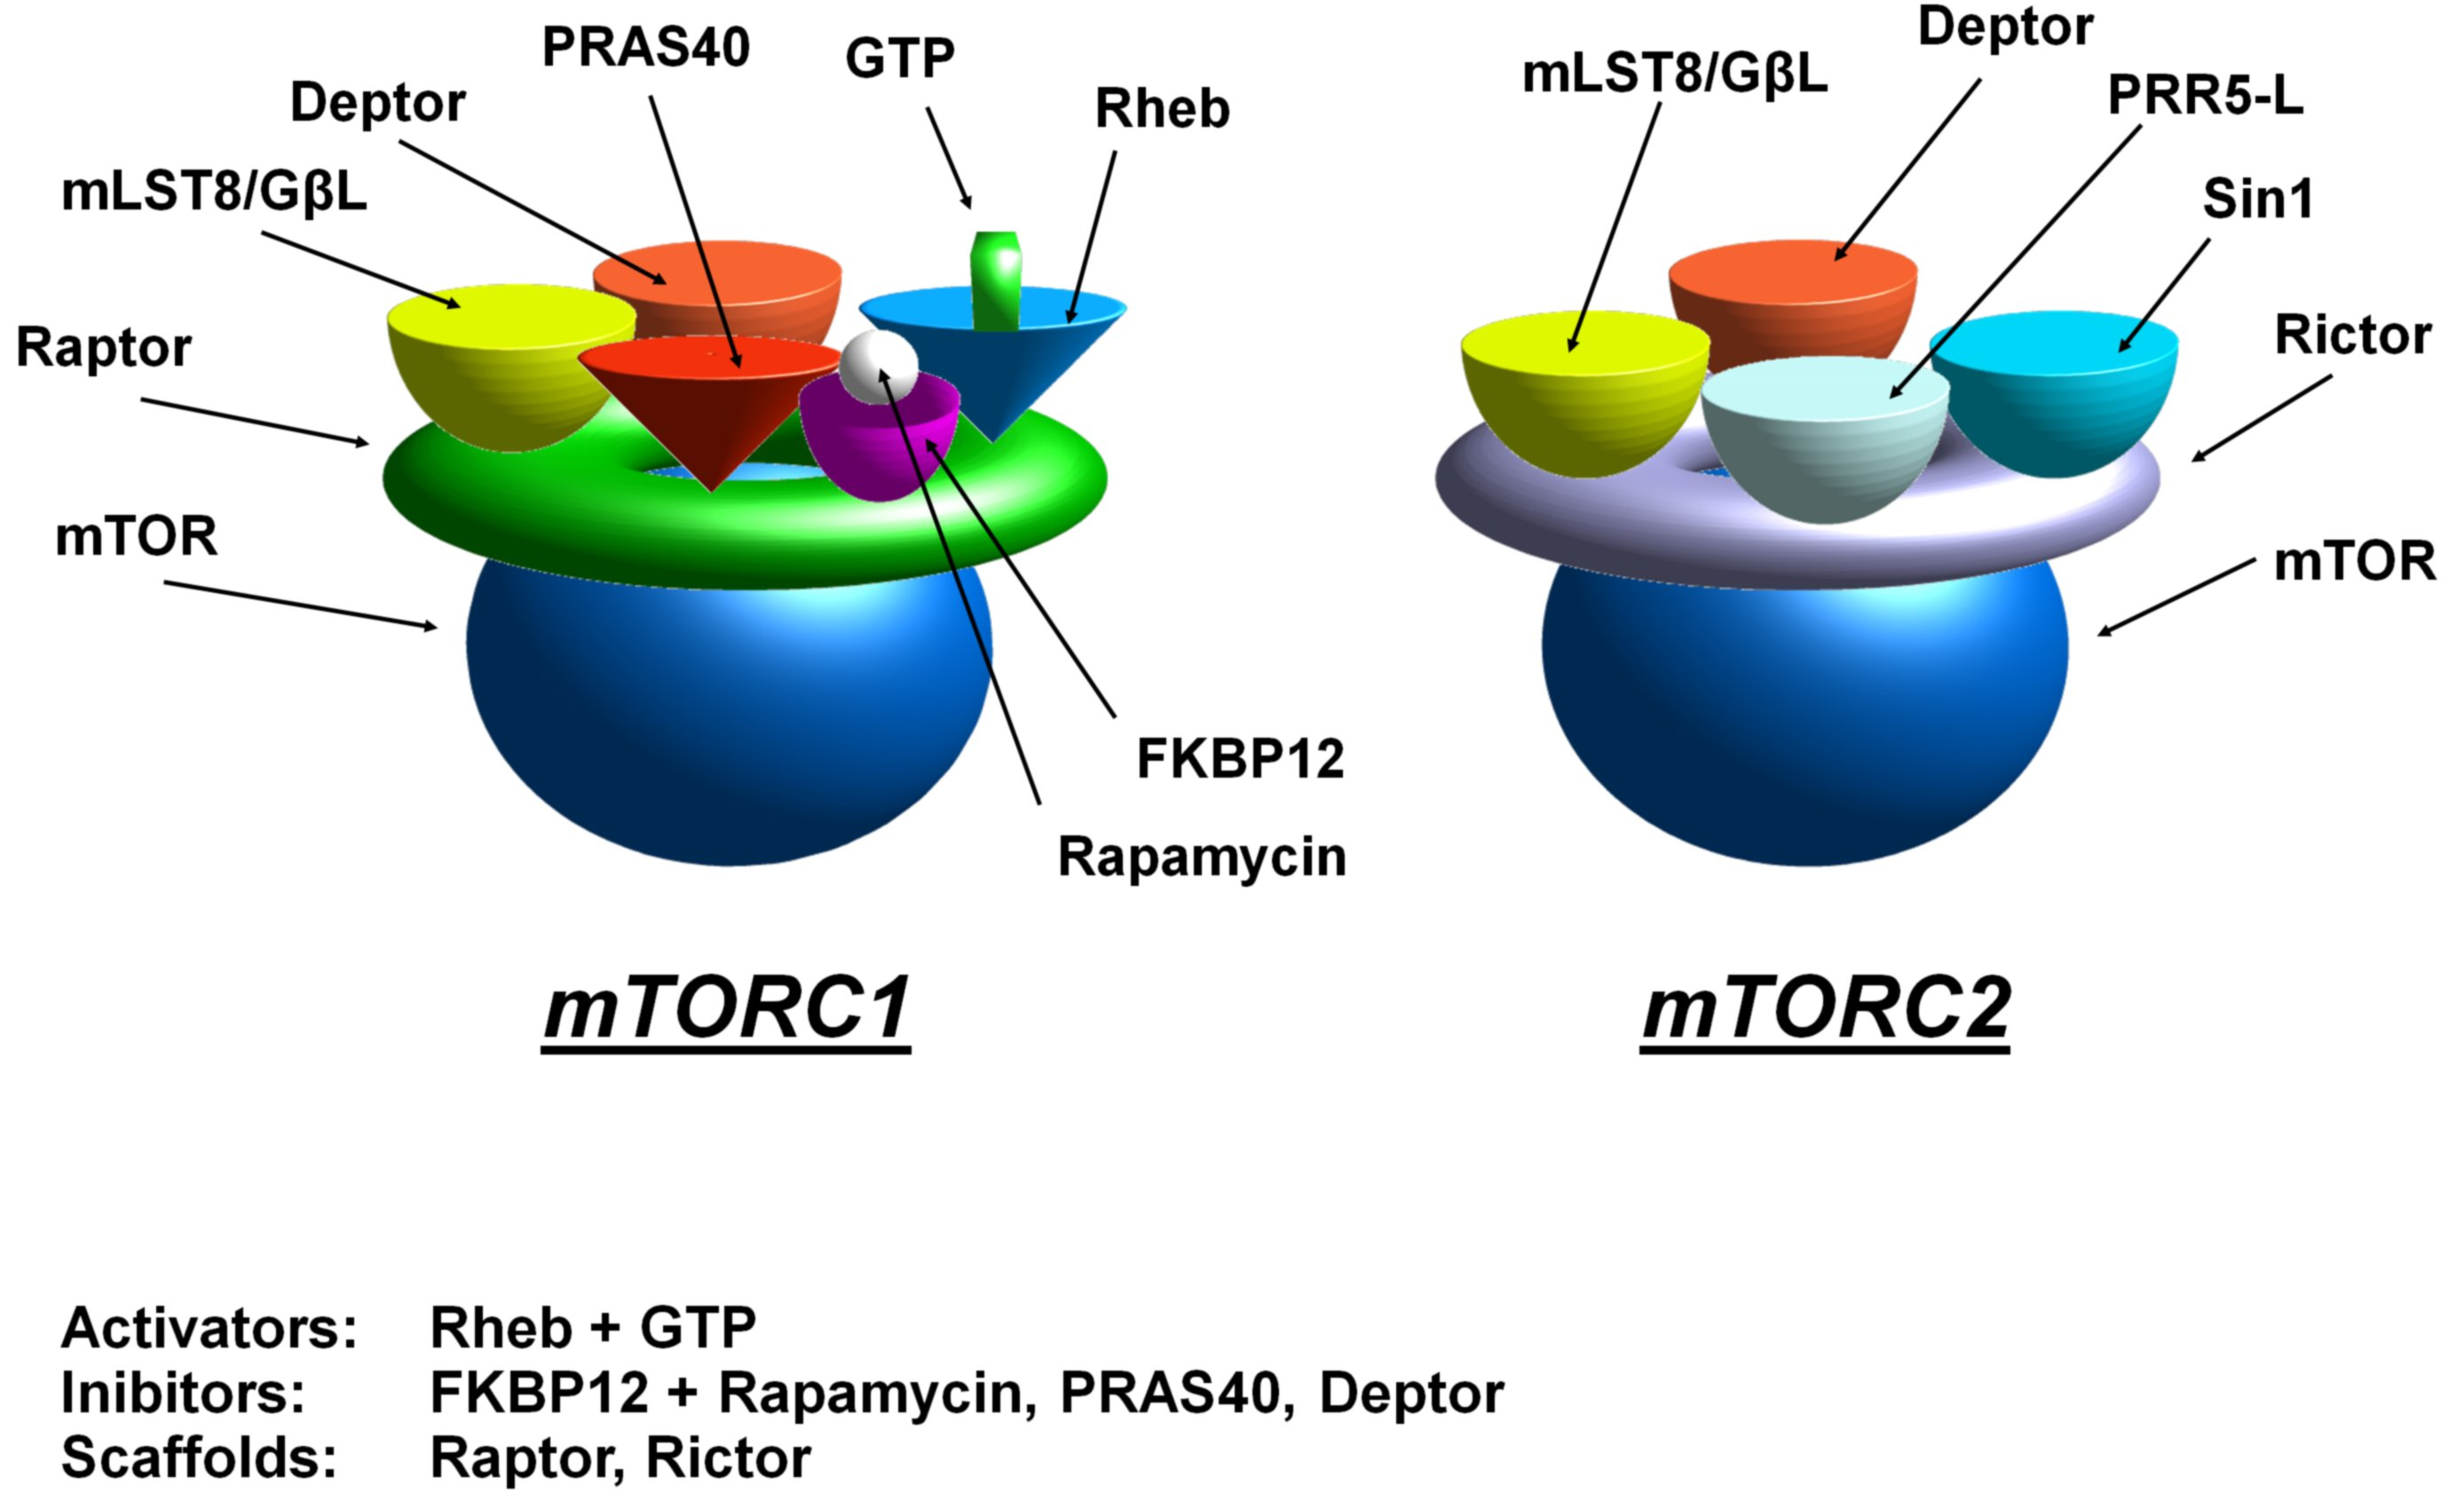
\includegraphics[scale=0.22]{mtor_complexes.jpg}
		\caption[mTOR complexes 1 and 2]{mTOR complexes 1 and 2. In mammals, the complexes mTORC1 and mTORC2 share mTOR, the mammalian LST8/G-protein $\beta$-subunit like protein (mLST8/G$\beta$L) and Deptor \citep{Peterson2009}. mLST8/G$\beta$L likely binds to the kinase domain of mTOR regulating its kinase activity. Deptor is known to have an inhibiting role in both complexes. A peculiar characteristic of mTORC1 is the binding with Raptor (Regulatory associated protein of mTOR). Raptor is known to be essential for the phosphorylation of mTORC1 downstream targets p70-S6K1 and 4E-BP1. It is supposed that it binds to the HEAT repeats of mTOR and it is sensitive to Rapamycin because it reduces its binding strength with mTOR in the presence of the drug. mTORC2 differs by containing Rictor (Rapamycin-insensitive companion of mTOR), the mammalian stress-activated protein kinase interacting protein 1 (mSIN1) \citep{Frias2006} and PRR5-L \citep{Woo2007}. mSIN1 is necessary for the binding between mTOR and Rictor, whereas 
PRR5 has not been found relevant. The detailed function of PRR5-L is still unknown.}
		\label{fig:mtor_complexes}
	\end{center}
\end{figure}
\begin{figure}[tb]
	\begin{center}
		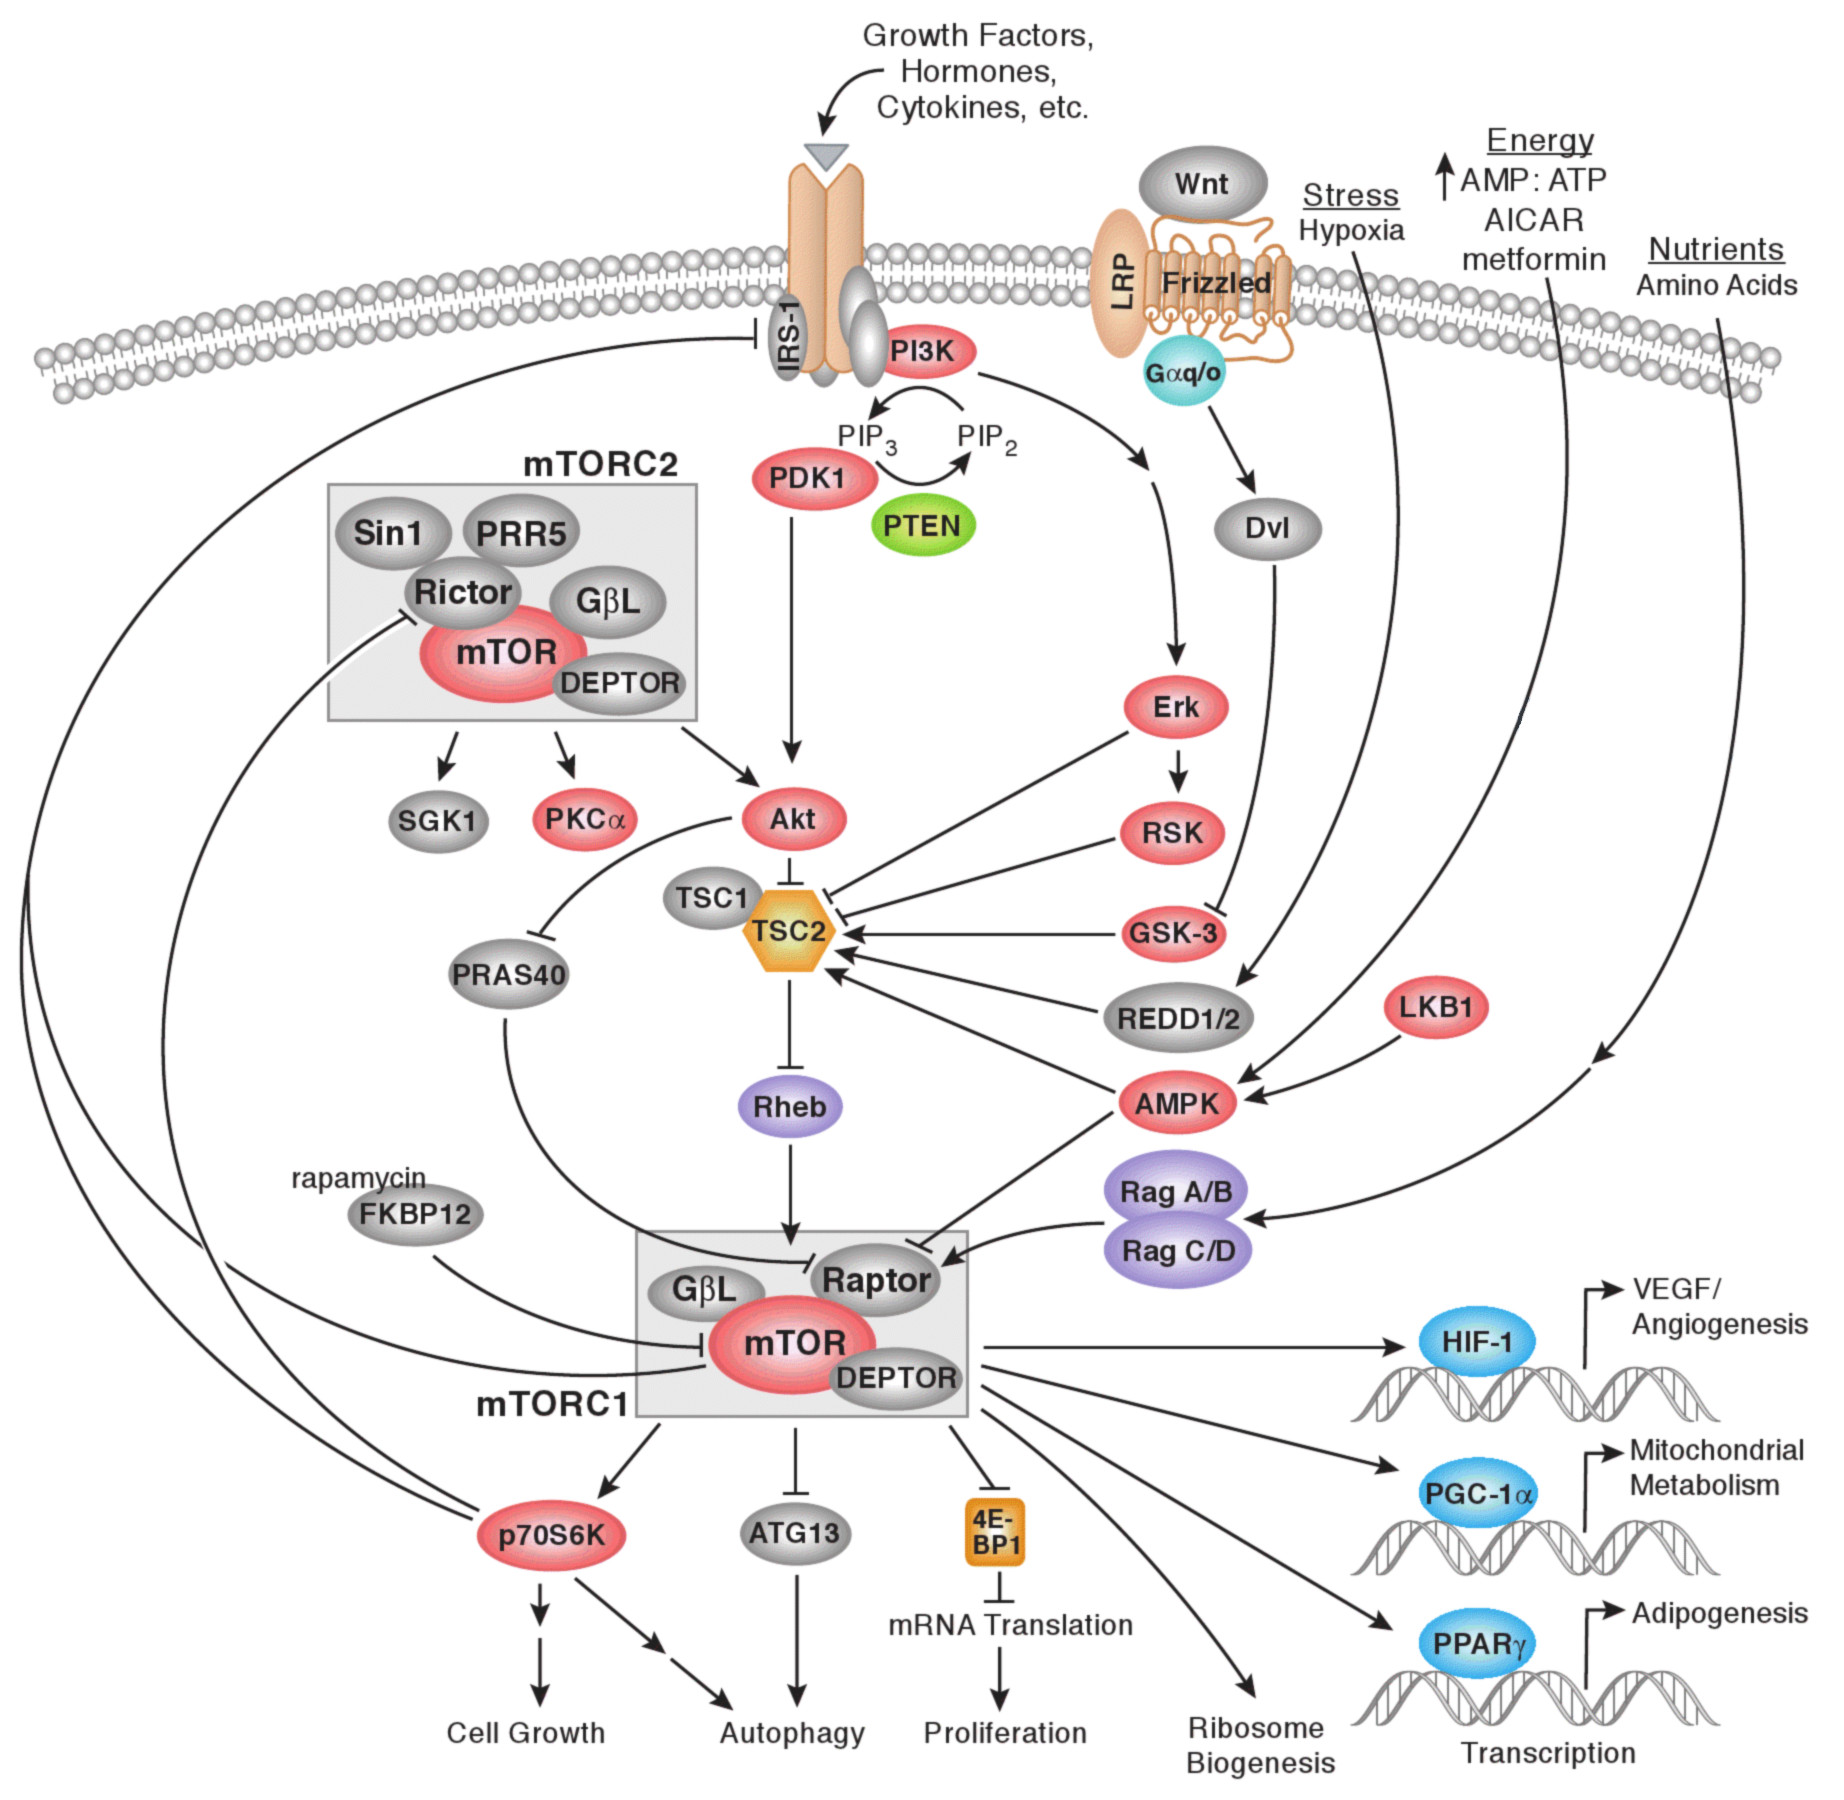
\includegraphics[scale=0.20]{mTor.jpg}
		\caption[mTOR signalling pathway]{The mTOR signalling network is complicated by the numerous inputs and interaction between signals. In addition, the network presents several negative and positive feedback loops and most of them are not completely understood. Understanding the relationships among the proteins and the mechanisms by which mTOR-dependent processes are regulated is of fundamental importance to enable intervention on numerous age-related diseases. New systems biology approaches, such as modelling, using phosphoproteomics data, are able to deal with the complexity of the network and predict both qualitative and quantitative regulations. (Source: Cell Signaling Technology$^\text{\textregistered}$ (CST), Inc., website: \url{http://www.cellsignal.com/}; proteins are linked to PhosphoSitePlus$^\text{\textregistered}$ (PSP), website: \url{http://www.phosphosite.org/} (CC BY-NC-SA 3.0) \citep{Hornbeck2012}).}
		\label{fig:mTOR}
	\end{center}
\end{figure}


\clearpage


% ------------------------------------------------------------------------


%%% Local Variables: 
%%% mode: latex
%%% TeX-master: "../thesis"
%%% End: 

\graphicspath{{Chapter4/Chapter4Figs/}}

\chapter{Systems biology for investigating mTOR network in ageing}
\label{chap:Systems biology for investigating mTOR network in ageing}
This chapter begins by presenting the main concepts of systems biology, from parameter estimation to advanced techniques of dynamical system theory. Finally, published work on systems modelling of the mammalian TOR network are described.

\section{Introduction to systems biology}
\label{sec:Introduction to systems biology}
Understanding the connections between proteins to form networks and determining the emergent properties of dynamical interactions has been a major focus of research in recent years. Due to the complexity of biological systems, the need for an appropriate level of abstraction in order to characterise the key signalling network governing cell behaviour is essential. An approach to address the problem is provided in the mathematical modelling of signalling pathways \citep{Kolch2005, Hughey2009}. So far, several key pathways have been modelled and simulated such as the epidermal growth factor (EGF) pathway \citep{Borisov2009, Schilling2009, Wang2009}, the insulin insulin-like pathway \citep{smith2010foxo_modelling, Brannmark2010, Nyman2012} or p53/MDM2 oscillation signalling \citep{GevaZatorsky2006, Proctor2008}. This chapter presents a concise introduction to systems biology and other more advanced techniques imported from dynamical systems theory with the aim of introducing the current mathematical models of 
the TOR network.\\

\subsection{Why systems biology?}
\label{subsec:Why systems biology?}
Before introducing the main concepts important for dynamic modelling in systems biology, I think it is reasonable to discuss what systems biology is and how it can improve our understanding in biological studies. Systems biology is not simply a means to replace expensive wet-experiments with dry alternatives. It would not be very useful to consider systems biology just as an additional tool to provide more evidence to support scientific findings. From this point of view, a systems biology approach does not reveal much more than using wet-experimental techniques.\\ 
The advantages of systems biology are multiple. Firstly, the system representation is an abstraction of the biological context, and therefore it is simpler to investigate. Systems biology offers an extraordinary possibility to represent our biological knowledge as an interconnected system using an appropriate formalism. Secondly, this system can be formally analysed from multiple perspectives using theories coming from other sciences such as mathematics and computer science (e.g. dynamical systems, optimisation, formal methods), and statistics (e.g. stochastic simulation of models). Thirdly, from these analyses, specific properties of the system can be extracted and formulated as modelling predictions which can be tested in the laboratory. Systems biology permits the biologist to selectively search those predictions (e.g. systematic sensitivity analysis of system components) as well as provides the user with new non-trivial results (e.g. system bifurcations at specific protein amounts). Moreover, the 
feasibility of obtaining these predictions is mainly due to fast numerical computing tools, which allows the user to perform high-throughput tasks which would be impossible for wet-experimentalists. 

\subsection{Model definition}
\label{subsec:Model definition}
Over the last 20 years, the necessity of creating a standard language for systems biology models has emerged. Systems Biology Markup Language (SBML) \citep{hucka2003systems} was developed as an XML standard aimed at porting systems biology models amongst different platforms and therefore increasing systems biology interoperability. In the field of molecular systems biology, a model is described as: (1) a set $S$ of species (e.g. unphosphorylated or phosphorylated proteins, complexes), (2) a set $R$ of reactions between species (e.g. phosphorylation, binding), (3) a set $I$ of inputs (e.g. insulin stimuli), and (4) a set $C$ of compartments (e.g. cytoplasm, nucleus). These biological models can be graphically represented using CellDesigner\footnote{\href{http://www.celldesigner.org/}{http://www.celldesigner.org/}} \citep{Funahashi2003, Funahashi2008}. Although this representation can be user-friendly, it hides the real representation of a model from a mathematical point of view. Instead, a mathematical 
representation explicitly offers the details for dealing with tasks such as parameter estimation and model quality analysis. A biological model can be described as follows:
\begin{align}
  \dot{\vec{x}}_{t,\theta} &= \vec{f}(\vec{x}_{t,\theta},\vec{u}_{t,\theta},\theta),\;\;\; \vec{x}_{t_{0},\theta} = \vec{x}_{0,\theta} \label{eq:ode_system} \\
  \vec{y}_{t,\theta} &= \vec{g}(\vec{x}_{t,\theta},\theta) + \vec{\epsilon} \label{eq:observable_function}
\end{align}
where \ref{eq:ode_system} is a system of Ordinary Differential Equations (ODEs) and \ref{eq:observable_function} describes the model observable variables. The ODE-based model is characterised by $n$ species $\vec{x}$ (e.g. protein concentrations), whose dynamics are dependent on $l$ input functions $\vec{u}$ (e.g. constant or impulse stimulation) and $j$ model parameters $\theta = \{\theta_1,\dots,\theta_j\}$ (e.g. protein initial concentrations, kinetic rates constants, scaling factors) over time $t = \{0,\dots,T\}$. The species in $\vec{x}$ which can be experimentally measured (e.g. by immunoblotting, mass spectrometry), are mapped into $m$ observable variables $\vec{y}$ by an observable function $\vec{g}$ and a measurement error $\epsilon \approx N(0,\sigma^{2}(d_{i,k}))$, where $\sigma^{2}(d_{i,k})$ is the variance of the $i$-th measurement at the time point $k$.

\subsection{Parameter estimation}
\label{subsec:Parameter estimation}
The choice of the observable variables depends on the measurements that can be feasibly measured in the laboratory. Once these  are collected, the model can be optimised in order to represent the experimental data within a certain error. Parameter estimation is the task in which the model parameters are established in order to reduce this error. Let ${d}_{i,k}$ and 
$y_{i,k,\theta}$ be the $i$-th data measurement and observable at the time point $k$ respectively, and $\sigma(d_{i,k})$ be the standard deviation for $d_{i,k}$, parameter estimation aims at measuring the distance between the model observables and the experimental data:
\begin{equation}
  \label{eq:chi_square}
  \chi^{2}(\theta) = \sum_{i=1}^{m} \sum_{k=0}^{T} \left(\frac{d_{i,k} - y_{i,k,\theta}}{\sigma(d_{i,k})}\right)^{2}
\end{equation}
and computing a solution, or assignment of values to the parameters $\theta$, which minimises such a distance:
\begin{equation}
  \label{eq:hat_theta}
  \hat{\theta} = \argmin_\theta {(\chi^{2}(\theta))} 
\end{equation}
Parameter estimation is therefore a problem of minimum optimisation. Optimisation algorithms can be classified into two classes: global and local algorithms. Global optimisation algorithms aim at finding the solution of minimum cost\footnote{Maximum cost in the case of maximum optimisation.} in the differential $\chi^2$ manifold\footnote{An $n$-dimensional manifold is a topological space having the property that the neighbourhood of each point approximates (formally, it is \emph{homeomorphic} to), the Euclidean space of dimension $n$, whereas this may not hold true globally.} $\mathcal{M}$ of the search space. Although these algorithms can be very accurate since the performed research is more extended, they usually have exponential time complexity. An additional problem is that they can stall on local minima, which may not be suitable as solutions. Examples of these algorithms are simulating annealing (SA) \citep{Kirkpatrick83, Corana1987}, genetic algorithms (GA) \citep{Baeck1993, Michalewicz1994, 
Mitchell1998, Baeck1997} and evolutionary programming (EP) \citep{Fogel1992, Baeck1993, Baeck1997}. Local optimisation algorithms focus on retrieving the minimum solution closest to the current assignation of parameter values. These algorithms usually permit to calculate a solution quickly, although this may not be optimal. Instances of this class are Trust Region (TR) \citep{Celis1984, Byrd1987, Yuan2000}, Levenberg-Marquardt (LM) \citep{Levenberg1944, Marquardt1963}, Steepest Descent (SD) \citep{Fogel1992} and Truncated-Newton (TN) \citep{Gill1981, Nash1984}. A common approach is to perform a global optimisation and then improve the solution quality by a local optimisation. These methods are implemented in several software tools for calibrating and analysing systems biology models. The models presented in this thesis were developed using Copasi\footnote{\href{http://www.copasi.org/}{http://www.copasi.org/}} \citep{Hoops2006} and the Matlab toolboxes Potterswheel\footnote{\href{http://www.potterswheel.de/}{
http://www.potterswheel.de/}} \citep{Maiwald2008, Hengl2007, Raue2009} and SBToolbox2\footnote{\href{http://www.sbtoolbox2.org/}{http://www.sbtoolbox2.org/}} \citep{Schmidt2006}. 
In the case of testing different biological hypotheses, each corresponding to a specific network structure, parameter estimation can be used for establishing a rank within these different networks, based on fitting quality. The $\chi^2$ measure is sufficient to define this hypothesis rank if the number of parameters is the same for each model, otherwise other measures taking into account the number of parameters, such as Akaike information criterion (AIC) \citep{Akaike1973} or Bayesian information criterion (BIC) \citep{Schwarz1978}, should be adopted. This hypothesis ranking can be useful as a means to predict likely network structure and to guide further experimental test that could discriminate between alternatives. An example of this approach can be found in \citep{Sonntag2012}.

\subsection{Identifiability analysis}
\label{subsec:Identifiability analysis}
In parameter estimation, two problems arise depending on model structure and data availability. The former concerns model structural non-identifiability \citep{Bellu2007, Raue2009, Raue2010, Balsa-Canto2010, Chis2011}. This type of non-identifiability happens when the model structure is not sufficiently mapped by the available data. For instance, if a sub-graph of the network is over-parameterised or there are not sufficient observables characterising those dynamics, that sub-component may result structurally non-identifiable. From a graphical point of view, structural non-identifiability is represented in the $|\theta|$-dimensional $\chi^2$ space as an unlimited plateau along the dimensions of the structurally non-identifiable parameters. Formally, assuming absence of measurement noise $\vec{\epsilon} = 0$, a subset of parameters $\eta \subset \theta$ is structurally non-identifiable if the overall $\chi^2$ remains constant for each assignment $a \in A$ to the parameters in $\eta$:
\begin{equation}
  \label{eq:structural_nonidentifiability_1}
  \{\forall \; \eta := a \; | \; \eta \subset \theta, a \in A\} \Rightarrow \chi^2(\theta) = const
\end{equation}
In other words, the parameters in $\theta$ cannot be uniquely determined due to a lack of observable information:
\begin{equation}
  \label{eq:structural_nonidentifiability_2}
  \vec{y}_{t,\eta} = \vec{g}(\vec{x}_{t,\eta},\eta) = \vec{0} \Rightarrow \chi^2(\theta) = const
\end{equation}
In practical terms, if a model is structurally non-identifiable, parameter estimation results are inconclusive, as infinite different solutions report the same $\chi^2$. Structural identifiability can be solved by altering the model structure or increasing the numbers of observable variables for the structurally non-identifiable sub-graph. Among the software for testing structural identifiability, the software GenSSI\footnote{\href{http://www.iim.csic.es/~genssi/}{http://www.iim.csic.es/$\sim$genssi/}} \citep{Balsa-Canto2010, Chis2011} was used in this thesis. GenSSI computes the successive $k$ orders of Lie derivatives of $\vec{g}$ with respect to the vector field $\vec{f}$, evaluated at the initial time $t=t_0$. In this generating series approach, GenSSI searches for a \emph{exhaustive summary}, which is a vector of the series coefficients, evaluated at the initial conditions, that only depends on the model parameters to estimate and identify. Then, GenSSI uses the exhaustive summary for computing 
solutions for the parameters $\theta$. If a unique solution is found, then the parameters are structurally globally identifiable; in the case of multiple solutions, the parameters are structurally locally identifiable. Finally, in the case of no solution, the parameters are structurally non-identifiable. \\
% GenSSI computes the successive $k$ orders of Lie derivatives of $\vec{g}$ 
%with respect to the vector field $\vec{f}$, evaluated at the initial time $t=t_0$:
% \begin{equation}
%   \label{eq:structural_nonidentifiability_3}
%   L_{\vec{f}_0} \dots L_{\vec{f}_k} \; \vec{g}(\vec{x}_{t, \theta},\theta, t)
% \end{equation}
% where such a Lie derivative is defined as:
% \begin{equation}
%   \label{eq:structural_nonidentifiability_4}
%   L_{\vec{f}} \; \vec{g}(\vec{x}_{t, \theta},\theta, t) = \sum_{j=1}^{n_x} 
%f_j(\vec{x}_{t, \theta}, \theta, t) \frac{\partial \vec{g}(\vec{x}_{t, \theta}, \theta, t)}{\partial x_{t, \theta, j}}
% \end{equation}
% Therefore, a model is structurally identifiable at Lie derivative of order $i$ if 
%a unique solution for $\theta$ can be obtained from the algebraic equation for $L_{\vec{f}_i}$. \\
Although a parameter is structural identifiable, it may still be practically non-identifiable \citep{Raue2009, Raue2010}. Practical non-identifiability depends on the amount or quality of data sets used to estimate model parameters and can therefore be solved by increasing or improving the measured data. In case of time-course-based experiments, this means that the collected time points are not enough in number or that their standard deviations are too big to allow the optimisation algorithm to infer clear time-dependent signalling trajectories. Therefore, practical identifiability concerns the problem of assessing finite confidence intervals for each parameter. A parameter $p$ is practically non-identifiable when its confidence interval is infinite, although there may exist a unique minimum for it. Graphically, the $\chi^2$ measured as a function of $p$, $\chi^2(p)$, is always lower than a desired confidence threshold $\Delta_\alpha$, in the neighbourhood of the parameter minimum $p_m$:
\begin{align}
  \label{eq:practical_nonidentifiability}
  \forall \; \delta \in \mathbb{R}^{+}: \; &\{\chi^2(p:=p_m) \le \chi^2(p:=p_m \pm \delta)\}, \\
  &\{\chi^2(p:=p_m - \delta) < \Delta_\alpha \vee \chi^2(p:=p_m + \delta) < \Delta_\alpha \} \notag 
\end{align}
This results in a deficiency in estimating a valid confidence interval for $p$ \citep{Raue2009, Raue2010, Raue2011, Kreutz2012}. A problem with this approach regards the choice of $\Delta_\alpha$. This threshold is defined as $\Delta_\alpha = \chi^2(\alpha, df)$, where $\chi^2(\alpha, df)$ is the $\chi^2$-distribution with confidence level $\alpha$ and degrees of freedom $df$ which corresponds to the number of parameter estimations. Therefore, an accurate $\Delta_\alpha$ depends on a sufficiently large number of precise parameter estimations which requires a considerable time to compute.\\ 
% Unfortunately, (1) the search space can contain several local minima and 
%(2) an optimisation algorithm can fail the convergence especially in the case of local optimisation algorithms. Whereas the second issue can be partially solved using global 
%optimisation algorithms, the first issue cannot be easily solved except by increasing 
%the amount of data, which augments the constraints in the parameter search space. 
%All these parameter estimations are included in the computation of $\Delta_\alpha$, 
%although several of them may not be reasonably accepted. This counting increases 
%the number of degrees of freedom for the $\chi^2$-distribution, leading to a reduction 
%of its variance, an increment of its the mean and a better approximation to a normal 
%distribution. As consequence, the threshold $\Delta_\alpha$ may result higher than 
%what is already sufficient for defining a confidence interval and therefore showing 
%the parameter as practically non-identifiable whereas it may be instead. 
%This situation is particularly likely in models with high number of parameters 
%because the parameter search space may dramatically increase its non-linearity 
%and therefore the number of local minima. For this reason, practical non-identifiability 
%was not investigated in the studies presented in this work. \\
In this thesis, the Potterswheel plugin Mean Optimal Transformations Analysis (MOTA) \citep{Hengl2007} was employed for detecting functionally related parameters and therefore solving structural non-identifiability issues in relation with data sets adopted for parameter estimation, in conjunction with a structural identifiability analysis theoretically performed using GenSSI. From a fit sequence of parameters, the MOTA algorithm returns the tuples of highly related parameters, permitting the user to fix independent parameters and estimate the remaining related parameters in the \emph{reduced} parameter space. These iterations of parameter estimation and fixing may eventually terminate leading to model identifiability, decreasing the variability of estimated parameters. In order to provide the user a graphical intuition of identifiability issue, Figure \ref{fig:landscape_identifiability} illustrates parameter non-identifiability through graphical $\chi^2$ landscape surface.

\subsection{Model simulation}
\label{subsec:Model simulations}
Before introducing a definition for simulation and describing the operations which can be done over a simulation, it is worth formalising the concept of algorithm. An algorithm $\mathcal{A}$ is a step-by-step procedure with an internal state $\mathcal{S}$ which receives an input $\mathcal{I}$, performs a list of instructions evolving $\mathcal{S}$ and returns an output $\mathcal{O}$ \citep{Cormen2009}:
\begin{equation}
  \label{eq:algorithm_definition}
  \mathcal{A}: (\mathcal{I},\mathcal{S}) \longrightarrow \mathcal{O}
\end{equation}
Therefore, a simulation can be defined as the task of reproducing a real problem, using an algorithm \citep{Malesani2004}. In this context, the interest is in simulating aspects of cellular behaviour, formally represented by mathematical models, and collecting information related to their temporal evolution. A mathematical model can be simulated deterministically or stochastically, depending on the type of algorithm used for reproducing its dynamical behaviour. 
For a certain input, a deterministic algorithm always returns the same output, reproducing the same internal state sequence. In other words, a deterministic algorithm does not contain any form of randomisation. An example of these algorithm is LSODA \citep{Hindmarsh1983, Petzold1983}. Stochastic algorithms differ as they include some form of randomisation, defined by a specific probability distribution, in their procedure \citep{Wilkinson2006}. This randomisation can be limited to the internal state sequence only or be propagated to the output. In the former case, a stochastic algorithm is called \emph{Las Vegas}\footnote{An instance of this class of algorithm is Randomised-Quicksort.} (LV), whereas in the latter case the algorithm is named \emph{Monte Carlo} (MC) \citep{Motwani1995, Cormen2009}. In the context of systems biology, the stochasticity of a biological context can be reproduced by MC stochastic algorithms, such as Gillespie \citep{Gillespie1976}, Gibson-Bruck \citep{Gibson2000}, Tau-Leap \citep{
Rathinam2003} or Runge-Kutta \citep{Kloeden1999}. This is of particular importance in the case of modelling gene transcription or low levels of protein amounts, since these systems are highly stochastic. The major drawback of stochastic simulations is their long computation-time as compared to deterministic simulations. For this reason, if the system stochasticity is low, a deterministic simulation may be more convenient for representing the dynamical behaviour of the model.

\subsection{Sensitivity analysis}
\label{subsec:Sensitivity analysis}
In mathematical modelling, establishing the influence of the parameters on overall behaviour is of fundamental importance to understand which of them play a more significant role then others \citep{Aldridge2006}. The analysis addressing this question is called sensitivity analysis. Sensitivity analysis is particularly useful in several areas. For instance, the detection of irrelevant parameters on the global dynamics may suggest model reduction \citep{Jia2008}, whereas assessing important ones may lead to new experimental design \citep{Cho2003}. Sensitivity analysis offers a means to explore the robustness of a system, as it shows how the dynamics change depending on parameter perturbation. There exist two types of sensitivity analysis: global and local. Global sensitivity analysis aims at retrieving multidimensional sensitivity operating multiple parameter changes. Local sensitivity analysis aims at exploring the domain of one parameter only and analysing the effect on the others \citep{Marino2008}.\\
The main concepts of sensitivity analysis are presented limiting the objective to linear models \citep{Saltelli2005}. A linear model can be represented as 
\begin{equation}
   \label{eq:linear_model}
   Y = \sum_{i=1}^{n} \Omega_i Z_i
\end{equation}
where $Y$ is the model output, $Z_i$ are uncertain input factors chosen from a normal distribution $Z_i \approx N(0,\sigma_{Z_i})$ and $\Omega_i$ are the coefficients for $Z_i$. $Y$ is also normally distributed $Y \approx N(0,\sigma_{Y})$, where $\sigma_Y = \sqrt{\sum_{i=1}^{n} \Omega_i^2 \sigma_{Z_i}^2 }$. Therefore, measuring a normalised sensitivity of $Z_i$ over $Y$ can be defined as:
\begin{equation}
  \label{eq:sensitivity_analysis}
  S_{Z_i}^{\sigma} = \frac{\sigma_{Z_i}}{\sigma_{Y}}\frac{\partial Y}{\partial Z_i}
\end{equation}
In case of a non-linear model, an extension of the previous calculation of sensitivity analysis based on MC methods can be found in \citep{Cho2003, Saltelli2005, Saltelli2008}.\\
Sensitivity analysis can be used in combination with model simulation. In fact, model simulations become particularly interesting when the initial conditions, such as the initial protein amounts or input stimuli, are changed. This type of simulation can reveal specific predictions, which can then be tested experimentally. For instance, reducing the amount of a protein species corresponds to a simulated knock-down, whereas increasing it represents a simulated over-expression. In the field of systems biology, cases of study involving this type of approach are \citep{Babu2004, Ihekwaba2004, Mahdavi2007, DallePezze2012a}. In this work, the term \emph{model perturbation} will be used to refer to a generic alteration of protein amount. Model perturbations can be interpreted as local sensitivity analyses performed on target species by varying their expression level. Of course, the number of protein species perturbed is not necessarily limited to one at a time. In fact, an advantage of systems modelling is the 
possibility to compute these dry-experiments relatively easily compared to wet-experiments in a laboratory. These predictions may reveal non-trivial dynamical changes at certain time points as well as at specific protein levels. Therefore, a biologist may use this information for reducing the number of experiments, as models can return optimal conditions for detecting differences or similarities, and extending biological knowledge, as models can predict completely new system behaviours. 

\section{Advanced analyses from dynamical systems theory}
\label{sec:Advanced analyses from dynamical systems theory}
Dynamical systems theory constitutes a powerful body of knowledge which can be used to investigate dynamical properties of the model. This section presents some of these analyses and their importance in the study of biological models.
\subsection{Steady-state analysis}
\label{subsec:Steady-state analysis}
After a certain amount of time, a system may reach a state characterised by invariability. This state is called steady state. A definition of steady state based on \citep{Garg2007, Ay2009} can be proposed as follows. Let $S$ be a set of states. $\forall s_i \in S$, $s_i$ is steady if and only if the following two conditions are verified:
\begin{align}
\label{eq:steady_state_analysis}
 1.\;\; & Succ(S) = S \\
 2.\;\; & \forall\; s_i,s_j \in S,\;\; \forall\; t \in T\;|\; t : s_i \rightarrow s_j,  \notag \\
        & \exists\; n \in \mathbb{N^{+}} finite \; | \; Prob(t^{(n)}(s_i)=s_i) = 1 \notag  
\end{align}
which means that (1) the set of the successors of $S$ is equal to $S$, and (2) for each visited $s_i \in S$ the probability of re-visiting $s_i$ is $1$ in a finite number of state transitions.\\
In other words, a steady state corresponds to a point at which the system reaches a condition of equilibrium or a fixed point from a mathematical point of view. This analysis is of particular interest for biological systems in order to elucidate the temporal length of specific dynamics and investigate the conditions leading to these steady states. Steady-state conditions also provide scientists with a starting point for analysing system behaviour at such states as illustrated in the following analyses.

\subsection{Stability analysis}
\label{subsec:Stability analysis}
An interesting question arising from the discovery of steady states in a dynamical model regards the system response upon a small perturbation of a steady state. Does this perturbed state move away from or towards its previous steady state? The analysis pertaining to this question is called stability analysis. These sort of questions are of particular interest in biological systems \citep{Thomson2009} and highly relevant in ageing. For example, a senescent cell can be seen as a cell staying in a specific steady state. As stochasticity increases with ageing \citep{FinchKirkwood_book2000, Bahar2006, Kirkwood2008}, the study of stability of a senescent steady state upon stochastic perturbations may reveal important information about the evolution of senescent cells. To provide an intuition of this analysis in the linear case\footnote{In case of non-linear systems, this linearisation technique can still be used although not generally.}, let us consider an $n$-dimensional linear system of ODEs\footnote{For 
simplicity, the Leibniz 
notation of derivative is used here.} \citep{Hirsch2004, Parks1992}:
\begin{align}
  \label{eq:stability_analysis1}
  \frac{dx_i}{dt} &= f_i(x_1, \dots, x_n), \;\;\; (i = 1,\dots, n)
\end{align}
and assume $\vec{s} = (s_1, \dots, s_n)$ be a steady state. Therefore:
\begin{align}
  \label{eq:stability_analysis2}
  f_i(s_1, \dots, s_n)=\frac{ds_i}{dt}=0, \;\;\; \forall\; i\; \in\; [1, n]
\end{align}
This system is now perturbed by a small perturbation $\vec{\rho}=(\rho_1, \dots, \rho_n)$, such that the new perturbed state is $\vec{s}^*=(s_1^*, \dots, s_n^*)=(s_1+\rho_1, \dots, s_n+\rho_n)$.\\
In order to determine whether the perturbed state $\vec{s}^*$ moves away from or towards $\vec{s}$, it is necessary to derive the System \ref{eq:stability_analysis1} at the perturbed state $\vec{s}^*$.
\begin{align}
  \label{eq:stability_analysis3}
  \frac{d(s_i + \rho_i)}{dt} = \frac{d\rho_i}{dt} &= \frac{ds_i^*}{dt}, \;\;\; (i = 1,\dots, n) \;\;\; \text{(by Formula \ref{eq:stability_analysis2})} \\
  &= f_i(s_1^*, \dots, s_n^*) \;\;\; \text{(by definition)}  \notag \\
  &= f_i(s_1+\rho_1, \dots, s_n+\rho_n) \;\;\; \text{(by substitution)}  \notag \\
  &= f_i(s_1, \dots, s_n) + \frac{\partial f_i}{\partial x_1}(s_1,\dots,s_n)\rho_1 + \dots +  \frac{\partial f_i}{\partial x_n}(s_1,\dots,s_n)\rho_n + \mathcal{T} \;\;\; \notag \\ 
  & \text{(Taylor series expansion)}  \notag \\
  &= \frac{\partial f_i}{\partial x_1}(s_1,\dots,s_n)\rho_1 + \dots +  \frac{\partial f_i}{\partial x_n}(s_1,\dots,s_n)\rho_n \;\;\; \text{(by Formula \ref{eq:stability_analysis2})}  \notag
\end{align}
where $\mathcal{T} = \mathcal{O}(\rho_1^n,\rho_2^n,\dots,\rho_1\dots \rho_n)$ are the Taylor series higher-order terms which can be neglected as $\vec{H}$ is assumed a small perturbation. Therefore, the evolution of the perturbation is determined by the following $n$-dimensional linear system:
\begin{align}
  \label{eq:stability_analysis4}
  \begin{pmatrix}
  \frac{d\rho_i}{dt} 
  \end{pmatrix}
 &=
  \begin{pmatrix}
   \frac{\partial f_i}{\partial x_j}(s_1,\dots,s_n)
  \end{pmatrix}
  \begin{pmatrix}
   \rho_i
  \end{pmatrix}, \;\;\; (i, j = 1,\dots, n)\\
 &= J \vec{\rho} \notag
\end{align}
where $J$ is the Jacobian matrix of the System \ref{eq:stability_analysis1} at the fixed point $\vec{s}$. At this stage, it is necessary to calculate the complex \emph{eigenvalues} $\lambda = (\lambda_1, \dots, \lambda_n)$, such that $J \vec{\rho} = \lambda\vec{\rho}$. Let $T = trace(J)$\footnote{The trace of a square matrix is the sum of the elements located on the main diagonal.} and $D = det(J)$, the classification for the fixed point $\vec{s}$ by linear stability analysis is summarised as follows:
\begin{itemize}
 \item Unstable fixed point (repellers or sources): \\$T > 0$, $D > 0$, $\forall \lambda_i \in \lambda: Re(\lambda_i)>0$
 \item Stable fixed point (attractors or sinks): \\$T < 0$, $D > 0$, $\forall \lambda_i \in \lambda: Re(\lambda_i)<0$
 \item Unstable fixed point (saddle points): \\$D < 0$, $\exists \lambda_i \in \lambda: Re(\lambda) > 0$
\end{itemize}
Additional study is required for the case in which there exist at least one eigenvalue with a null real part \citep{Hirsch2004}.


\subsection{Bifurcation analysis} 
\label{subsec:Bifurcation analysis}
Bifurcation analysis offers a way to detect and characterise qualitative behaviour variations around a selected steady state of a model. This leads to the investigation of signal trajectory changes by systematically exploring the domain of one or more model parameters. In conjunction with stability analysis, bifurcation analysis enables one to map the possible states of a system and how this system can switch between them \citep{Aldridge2006}. 
Biological systems are typically characterised by multiple steady states. Therefore, understanding the conditions by which a system transits from one steady state to another one is important, especially when investigating biological states which are apparently irreversible. Many age-related diseases discussed in Section \ref{sec:TOR in age-related diseases} are defined by a cellular dysregulation which denies the system to restore its normal functionality. More generally, since ageing itself has been considered an irreversible process, it would be interesting to investigate under which conditions, a senescent phenotype may \emph{resume} a pre-ageing phenotype or at least remain locked at the current state. Bifurcation analysis provides an exceptional tool for treating and possibly answering these biological questions. Due to the large body of bifurcation theory, this section only provides an overview of it in order to give a graphical interpretation insight of the analysis without dealing with the 
mathematical details. More formal introductions of this theory can be found in \citep{borisuk1997, Hirsch2004}.\\ 
The study of bifurcations concerns the individualisation of \emph{bifurcation points} which are the points corresponding to specific parameter values at which a system undergoes a qualitative state change. A bifurcation is said to be \emph{local} if the bifurcation point is located in the neighbourhood of a fixed point, also called steady-state, or periodic solution, otherwise it is called \emph{global}. The number of parameters which must be specified in order to detect a bifurcation is called \emph{co-dimension}. To clarify these concepts, two instances of bifurcation are graphically represented in Figure \ref{fig:tyson2003_fig1_adapted}. \\
A system containing a bifurcation $b$ can always be reduced to its \emph{normal form}, which is the simplest system preserving $b$. Local bifurcations requires that the perturbation of a parameter alters the stability of a fixed point, that is that the real part of an eigenvalue in $J$ passes through 0\footnote{This typology of fixed points are called non-hyperbolic.}. Because of this, a common approach when working on higher dimensional models consists of calculating the normal form of such a model and then focusing on the \emph{eigenvectors} in the \emph{centre} subspace\footnote{\emph{Centres} are fixed points for which the eigenvalue of $J$ are purely imaginary. For these fixed points, the solution within their subspace do not converge to nor diverge from them.}, ignoring the \emph{stable} and \emph{unstable} subspaces \citep{borisuk1997, borisuk1998}. Conversely, a pragmatic way of mapping the states of a system is by systematically sampling the parameter space and then looking for 
qualitative differences in the phase space \citep{Araujo2007, Wang2010bifurcation}. Of course this approach is only suitable for lower-dimensional models. 

\subsection{Lyapunov exponents} 
\label{subsection:Lyapunov exponents}
When studying a dynamical system, it may be of interest to investigate qualitative behaviour changes over time \citep{Aldridge2006}. A  measure used for characterising this quantity is the vector of \emph{Lyapunov exponents}. This type of analysis allows one to determine specific attractors in the system evolution as well as the rate of these dynamical changes. Interestingly, the determination of this rate also provides an estimation of the rate of entropy production of the system. In a biological context, Lyapunov exponents can be used to prove whether a biological system is stable, asymptotically stable or presents some form of chaotic behaviour. To provide an intuition of this analysis, let us consider a reduced system composed of two points $x_1(t)$ and $x_2(t)$ in the state space of a dynamical system, assuming that they are very close together at initial time $t=0$. Therefore, the objective is to study how these two points evolve over time. The trajectories individualised by these points diverge at a 
rate estimated by:
\begin{align}
  \label{eq:Lyapunov_exponents1}
  |x_1(t) - x_2(t)| \approx e^{\lambda t}|x_1(0) - x_2(0)|
\end{align}
where $\lambda$ is a Lyapunov exponent. Since this exponent, which resembles a separation rate of trajectories, depends on the considered dimensions of the phase space, a general dynamical system evolving in an $n$-dimensional space $\mathbb{R}^n$ will be characterised by a \emph{spectrum of Lyapunov exponents} $\{\lambda_1, \dots, \lambda_n\}$. Moreover, as a spectrum depends on the positions of the trajectories at time $t=0$, different spectra of Lyapunov exponents can be found by changing the initial time. Therefore, for each reached attractor, a particular spectrum can be calculated.\\
Among the Lyapunov exponents of a selected spectrum, the largest one, defined using the previous example as 
\begin{align}
  \label{eq:Lyapunov_exponents2}
  \lim_{t\to+\infty} \frac{1}{t} \ln \frac{|x_1(t) - x_2(t)|}{|x_1(0) - x_2(0)|} %lim for t \rightarrow \infinite$}
\end{align}
permits to obtain an overview of the global behaviour of the system, whereas the signs of all the exponents in the spectrum provides information about the type attractor \citep{Parks1992}. In more detail, assuming that a system of the first approximation is regular\footnote{This condition is substantial \citep{Leonov2007} as shown in \citep{Perron1930} by counter-example.}, such as systems characterised by constant or periodic coefficients \citep{Leonov2007, Kuznetsov2008}, if all its Lyapunov exponents are negative, then the system is asymptotically Lyapunov stable, otherwise some form of chaotic behaviour occurs \citep{Lyapunov1892, Parks1992, Kuznetsov2008}. This knowledge can be important in characterising the system in long-term dynamics. Furthermore, it may be significant to characterise the topologies of attractors to which a system may evolve and study how these states mutate in presence of stochasticity. 


% \subsection{Singular perturbations}
% \label{subsec:Singular perturbations}

\section{mTOR dynamical models}
\label{sec:mTOR dynamical models}
Interest in the mTOR network has increased in the recent years but only few, often incomplete, models have been developed. In this section, an overview of these existing mTOR models are presented.

\subsection{Model of Jain and Bhalla}
\label{subsec:Model of Jain and Bhalla}
In \citep{Jain2009}, the authors proposed a signalling network model involving growth factors such as brain-derived neurotrophic factor (BDNF) and neurotransmitters such as glutamate to predict mTOR activity and downstream effects. The focus was the analysis of protein synthesis in dendrites which is fundamental for memory formation. Their model predicted levels of protein synthesis from the complex formed by eiF4F and S6, which are downstream targets of mTORC1. Three inputs were considered: a BDNF pathway which propagates the signal to mTORC1, metabotropic glutamate which binds to its receptor and stimulates Akt, and ionotropic glutamate and its relative calcium ($Ca^{2+}$) production. Once calcium levels are increased, the signal activates the ERK pathway by stimulating p21/Ras protein and MAPK, and the calcium-calmodulin type III kinase (CaMKIII) by inhibiting eukaryotic elongation factor-2 (eEF2). The model was parameterised using previously published experimental data, combined with published models of 
$Ca^{2+}$ and 
MAPK signalling.\\
The authors found that the protein synthesis is primarily due to the BDNF signal and that MAPK serves to increase responses further. Three positive feedbacks related to BDNF, 40S and eEF2 were implemented. From the introduction of positive feedback, the authors identified bistability which is however not sufficient to declare that the system exhibits an inner switch-like behaviour because the model could not show bistability when fixed fractions of the total synthesised proteins were considered for each kind of feedback molecule.\\
The implemented model was based on about 130 molecular species. However, it does not consider mTORC2 nor any negative feedbacks. Also, the mTORC1 inhibiting-substrate protein PRAS40 is not included. The model lacks negative signals which are common in biological systems and it appears rather unlikely that there is no negative feedback in biological neuronal systems, since neuronal transmission is tightly controlled.

\subsection{Model of Vinod and Venkatesh}
\label{subsec:Model of Vinod and Venkatesh}
In \citep{Vinod2009}, a model of mTOR activated by amino acids and insulin growth factors (IGF) was proposed. Amino acids are necessary for the mTOR activity and nutrient starvation is recognised to inhibit mTOR even when stimulated by growth factors such as insulin. In the developed model, amino acids regulate the activity of Class III PI3K or hVps34, regulating mTORC1 and p70-S6K. The insulin pathway involves the classic IRS1/PI3K/Akt/TSCs pathway. The model also introduces PRAS40 and FKBP38 as mTORC1 inhibitors. The authors mentioned mTORC2 in their model, although it is not associated with any other protein. The insulin pathway is parameterised by using data from an earlier more specific insulin model \citep{Giri2004}. Other parameters are taken from literature or assumed.\\
The authors found that amino acids are necessary to regulate Rheb, mTORC1 and PRAS40. In the absence of amino acids, their model predicted that an overexpression of the GTP form of Rheb is able to achieve the same effects of a stimulation based on amino acids.\\
In this ODE-based model, many parameters are assumed without any connection with experimental data and robust experimental validation and testing of the model predictions is missing.

\subsection{Model of Borisov et al.}
\label{subsec:Model of Borisov et al.}
The model proposed by \citep{Borisov2009} studies the interactions between the insulin and epidermal growth factor (IGF and EGF), comprising positive and negative feedbacks. The PI3K/Akt pathway is activated by either IGFR directly or by EGFR indirectly involving the phosphorylation of Grb2-associated binder 1 (GAB1). The Ras/ERK pathway is activated directly by EGFR which can either bind with the complex Grb2-SOS or with Shc. The same pathway can also be activated indirectly by IRS1 binding with Grb2-SOS. There are numerous positive and negative feedbacks from IGFR and EGFR downstreams, such as mTORC1, GSK3 and ERK. These phosphorylate and inhibit proteins such as IRS1, Akt and GAB1 which then interrupt or increase the signal propagation. By using an experimental parameterisation, this model shows how insulin enhances the activation of the MAPK/ERK pathway whenever applied in combination with EGF. This cooperation between the two pathways is demonstrated to occur both upstream and at the level of p21/c-Raf (Ras/Raf) level.\\
The model predicts that the stimulation of insulin is only a weak indirect activator of EGF pathway. However, a synergistic effect was found in the presence of a co-stimulation of both EGF and IGF due to crosstalk interactions. This synergy becomes insignificant at saturating EGF levels.\\
The model is made of nearly 80 species and 110 reactions. In order to fit and customise the model, data from \emph{in vitro} and \emph{in vivo} experiments are used in combination with previously published models by the same authors. All performed simulations of the model were deterministic. Although an explicit identifiability analysis of the estimated parameters is missing, the authors reported numerous model predictions opportunely validated with experimental data. This continuous link between \emph{in silico} and \emph{in vitro} experiments is of crucial importance in systems biology in order to increase the confidence of the model predictions. This study therefore offers a clear example of how modelling-experimental-based approaches should work.

\subsection{Model of Araujo et al.}
\label{subsec:Model of Araujo et al.}
In \citep{Araujo2007}, dynamical systems properties were investigated in a reduced model of the TOR network. In this study, a minimal model comprising of just IRS1, Akt and mTORC1 was generated in order to determine and map dynamical states of the system to healthy or cancer phenotypes. A cancer phenotype was modelled by an hyper-activated positive feedback loop driven by Akt to the IRS1 \citep{Gual2005}. The authors analysed the case of no-treatment versus the cases of single inhibitory treatments of mTOR, Akt or IRS1 by gradually perturbing the input signal, represented by insulin. Therefore, their approach illustrates network behaviours under different conditions upon parameter perturbation, using techniques based on dynamical systems theory. In case of no-treatment or inhibition of mTOR, or IRS1, the hyper-activated positive feedback loop showed a one-way switch represented by bi-stability at low levels of input stimulus and by a monostable high response above a critical threshold of input level. In the 
case of inhibition of Akt, the one-way switch was converted to a two-way toggle switch (for a graphical representation of these two bifurcations, see Figure \ref{fig:tyson2003_fig1_adapted}), permitting to control the positive feedback intensity by reducing the input stimulus. Finally, the authors showed that these dynamical switches can be removed by a treatment inhibiting the positive interaction between Akt and IRS1\footnote{IRS1 can also activate a positive feedback loop through its downstream target PKC as shown in \ref{subsec:PKC}.}. This treatment would act to restore the functionality of the negative feedback loop, and a response control to different stimulus levels, changing the disease phenotype. Recently, \citet{Wang2010bifurcation} showed that it is highly likely that only two dynamical states are possible for the model defined by \citep{Araujo2007}. This result was achieved by systematically exploring the model $6$-dimensional parameter space and mapping types of 
signalling responses, without using any other experimental data sets. Although such reduced model may seem too simplistic to approximate the corresponding biological TOR network, it includes the two most important components of the network and the negative feedback loop. Therefore, the applied abstraction is correct because it contains all the necessary information for determining TOR regulatory mechanism, conserving the network behaviour. This study also represents a clear example of how dynamical systems theory can provide systems biologist with new interesting insights of a case of study, herein a simplified TOR network.

\subsection{Model of Caron et al.}
\label{subsec:Model of Caron et al.}
The knowledge about the mammalian TOR network has been steadily increasing in the last few years. \citet{Caron2010} reviewed this information in Systems Biology Graphical Notation (SBGN) \citep{lenovere2009systems} and SBML \citep{hucka2003systems} using the software CellDesigner \citep{Funahashi2003, Funahashi2008}. In contrast to the previous models, this work does not involve any time-course experimental data, parameter estimation or model simulation. Instead, the objective was to link all the pathways interacting with the complexes mTORC1 or mTORC2 into a single network. This integrative model comprises a total number of $777$ reactions and $964$ species, incorporating the upstream and downstream signalling of mTOR. In more detail, the included upstream signalling modules are growth factors, nutrients, energy, hypoxia, WNT, TNF, whereas the downstream modules comprise autophagy, protein folding, rRNA and ribosome biogenesis, cap-dependent translation, mitochondrial metabolism, cytoskeleton dynamic, transcription and cell cycle. The authors also generated a simplified network extracting the most relevant information from their extended model and highlighting the activation and inhibition reactions. In addition, a version is available as a web-service\footnote{Web-service: \href{http://sblab.celldesigner.org/Payao10/bin/}{http://sblab.celldesigner.org/Payao10/bin/}} and continuously updated. This review represents the first attempt to reproduce the TOR network on a large scale and therefore it undoubtedly constitutes an important achievement in systems biology.


\section{Figures}
\label{chap4:Figures}

\clearpage

\begin{figure}[tb]
	\begin{center}
% 		\textbf{A}
% 		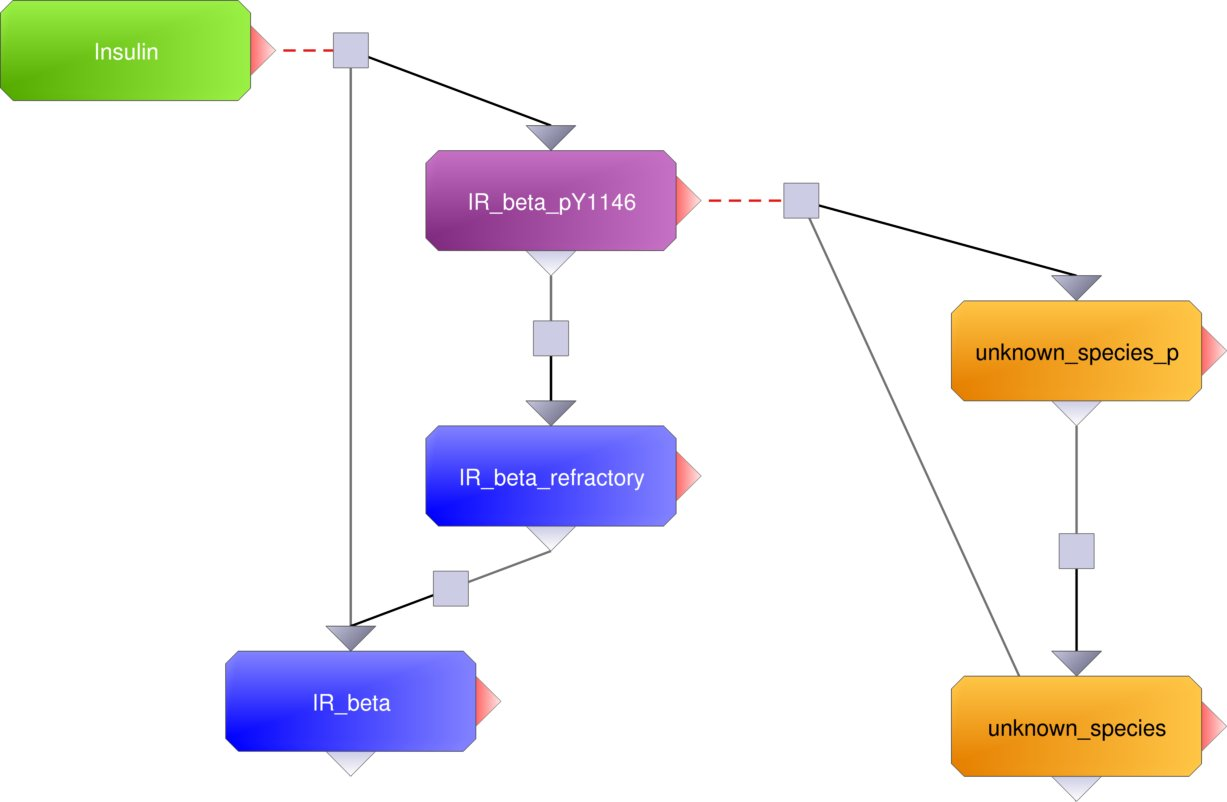
\includegraphics[scale=1.2]{insulin_receptor.jpg}
% 		\hfill
% 		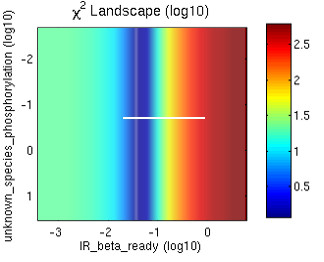
\includegraphics[scale=0.70]{structural_nonidentifiability_new.jpg}
% 		\textbf{B}
% 		\hfill
% 		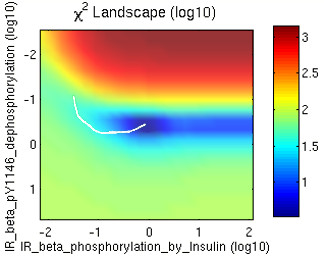
\includegraphics[scale=0.70]{practical_nonidentifiability_new.jpg}
% 		\textbf{C}
% 		\hfill
% 		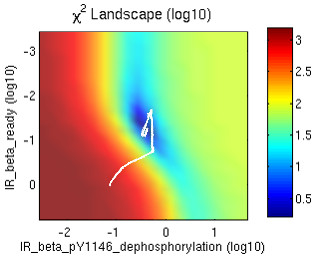
\includegraphics[scale=0.70]{identifiability_new.jpg}
% 		\textbf{D}
% 		\hfill
 		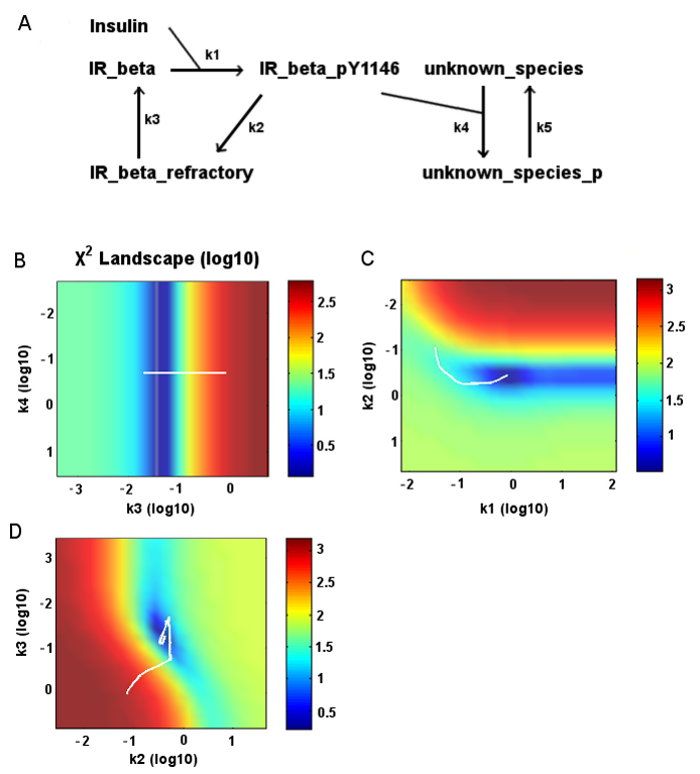
\includegraphics[width=350px]{ir_beta_model_identifiability.png}
		\caption[Graphical visualisation of parameter non-identifiability]{Graphical visualisation of parameter non-identifiability by $\log_{10}(\chi^2)$ landscape (darker colour correspond to parameter minimum). (A) Graphical mini-model of the insulin receptor with an additional unknown species. In this example, the only observable species is IR\_beta\_pY1146 which is phosphorylated by Insulin. IR\_beta\_pY1146 is responsible for the phosphorylation of unknown\_species, a species for which no information is available. (B) Structural non-identifiability for the parameter regulating the phosphorylation of unknown\_species. This parameter is clearly structurally non-identifiable as its dynamics are not mapped by any data. This parameter does not affect the search of solutions in the $\log_{10}(\chi^2)$ landscape. (C) Practical non-identifiability shown as an infinite upper bound confidence interval slightly above the parameter minimum (see blue $\chi^2$ region on the right). (D) Parameter identifiability. The 
parameter is clearly identifiable showing a well defined minimum and a confidence region. White line indicates the convergence path to a solution in the $\log_{10}(\chi^2)$ landscape.}
		\label{fig:landscape_identifiability}
	\end{center}
\end{figure}

\begin{figure}[tb]
	\begin{center}
		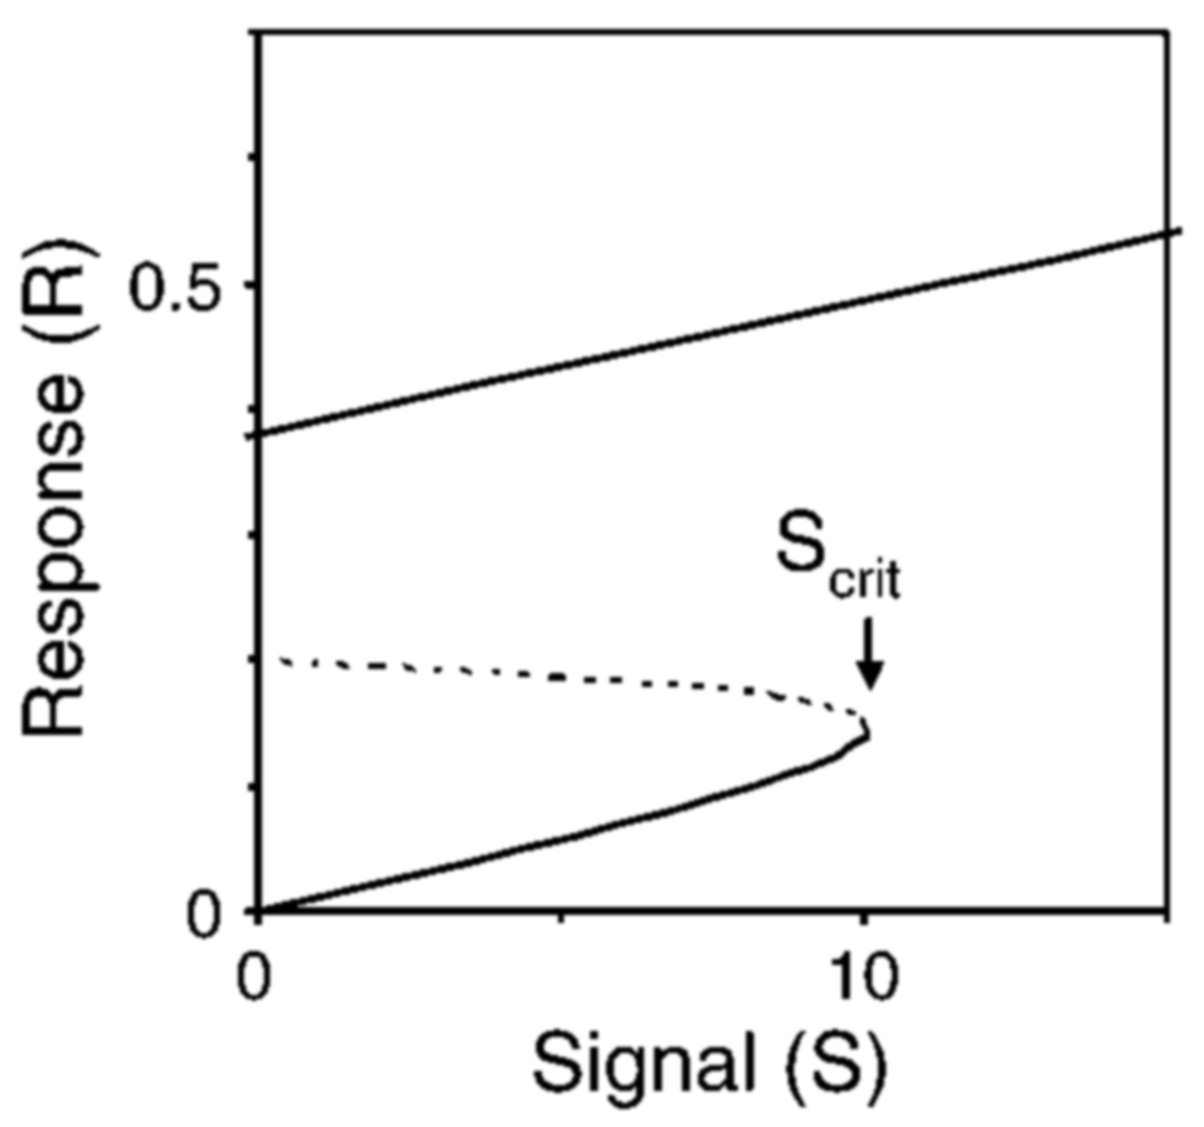
\includegraphics[scale=0.2]{tyson2003_fig1_adapted1.jpg}
		\textbf{A}
		\hfill
		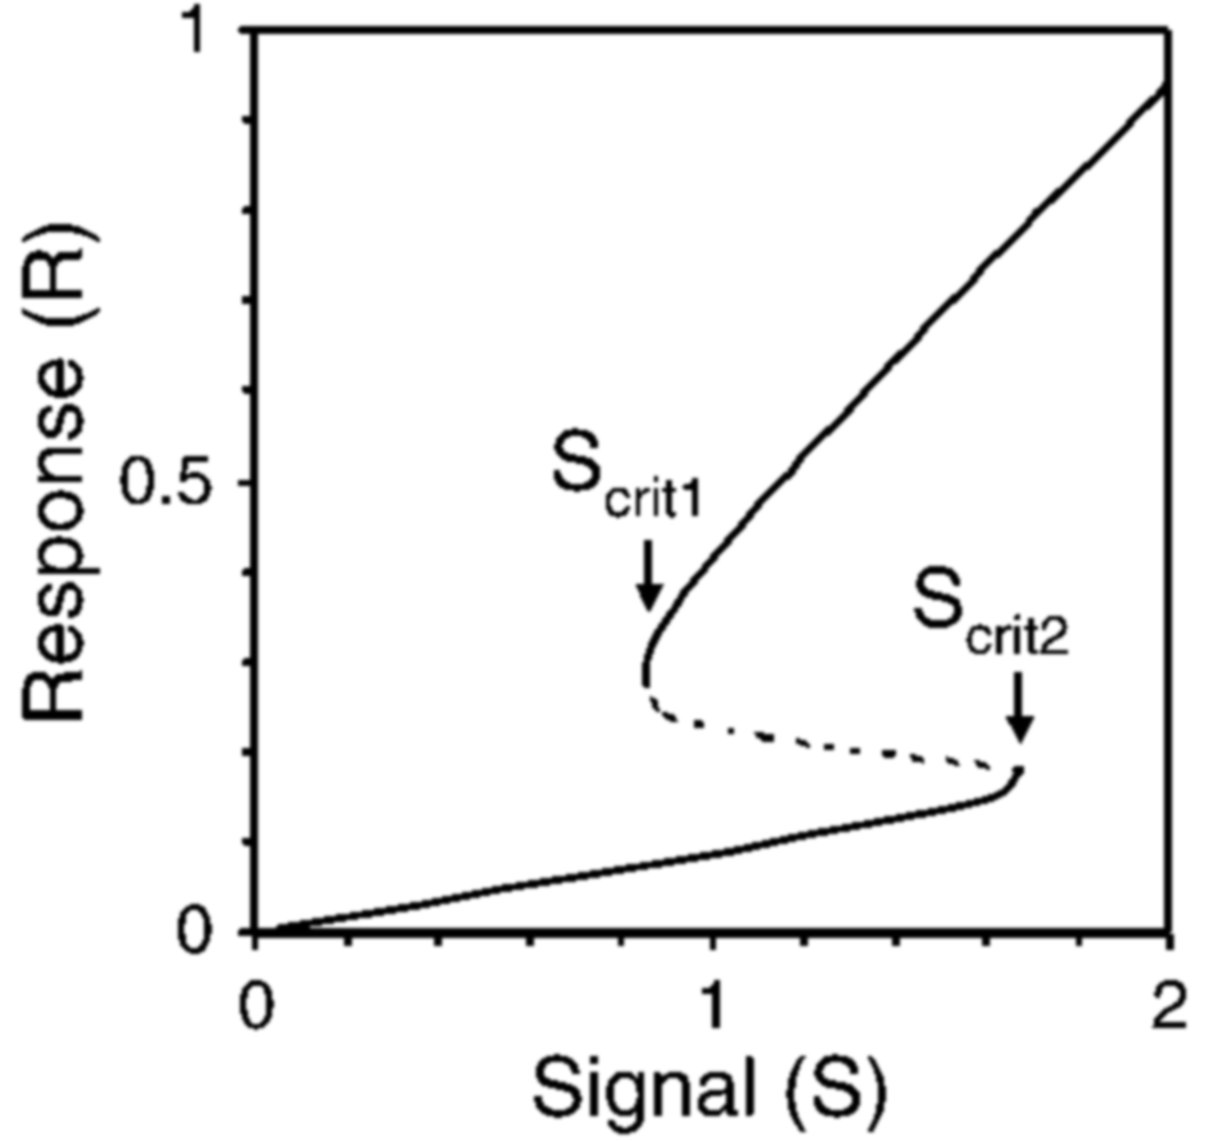
\includegraphics[scale=0.2]{tyson2003_fig1_adapted2.jpg}
		\textbf{B}
		\hfill
		\caption[Graphical examples of bifurcations.]{Graphical examples of bifurcations. (A) One-way switch bifurcation. At low levels of input stimulus, the system shows a bistable signalling response. After reaching a critical point, or bifurcation point, $S_{crit}$, the previous response dramatically changes into a monostable elevated response. This signalling response is characterised by two steady states (a low one and a high one) separated by an unstable state. However, the high steady state is the only one which persist above a certain threshold $S_{crit}$ of input stimulus, since the system is not able to restore its signalling response to the low steady-state. (B) Two-way toggle switch bifurcation. This type of bifurcation presents two bifurcation points, called $S_{crit1}$ and $S_{crit2}$, depending on both the strength and history of the input stimulus. This dependency of the response on the previous and current levels of the input stimulus represents the reason why these switches are also called \emph{
hysteresis}. In contrast to the previous case, this bifurcation permits to free the system from a constitutively activated response, since this one can be reduced by altering the signal strength. Adapted from \citep[Fig. 1]{Tyson2003}.}
		\label{fig:tyson2003_fig1_adapted}
	\end{center}
\end{figure}


\clearpage



%%% Local Variables: 
%%% mode: latex
%%% TeX-master: "../thesis"
%%% End: 
 
\graphicspath{{Chapter5/Chapter5Figs/}}

\chapter{A dynamical network model of mTOR signalling reveals TSC-independent mTORC2 regulation}
\label{chap:A dynamical network model of mTOR signalling reveals TSC-independent mTORC2 regulation}
This chapter describes a systems biology-based investigation of mTORC2 regulation as described in \citep{DallePezze2012a}. The results here focus on the modelling point of view and only include \emph{in vitro} experimental work necessary for model validation and test. All the \emph{in vitro} data included in this project were collected by Annika Sonntag, PhD student supervised by Dr Kathrin Thedieck, Department of Bioinformatics and Molecular Genetics, Freiburg University, Germany. A copy of the published work, which includes the \emph{in vitro} experimental data used for parameterising and testing the model, is attached in Appendix \ref{appendixA}.

\section{Introduction}
\label{paper1-sec:Introduction}
In this project an insulin-mTOR network model integrating both mTORC1 and mTORC2 was built and used to investigate alternative mTORC2 activation mechanisms. In contrast to mTORC1, little is known about mTORC2 upstream regulation (see Section \ref{sec:Upstream signalling pathways of mTOR}). mTORC2 is mainly regulated by growth factors (see Section \ref{subsec:The insulin insulin-like signalling pathway}), but the molecular mechanism has not yet determined. \\
Many substrates of mTORC2 are proteins belonging to the family of AGC kinases (see Sections \ref{subsec:mTOR-dependent regulation of AGC kinases}, \ref{sec:Downstream targets of mTORC2}). Using these AGC kinases as indicators of mTORC2 activity, the TSC1/TSC2 complex has been implicated in mTORC2 activation by insulin. It was found that TSC1/TSC2 inhibition reduces phosphorylation of Akt at S473 \citep{Inoki2005, Huang2008, Huang2009complex, Huang2009signaling}, which contrasted with TSC1/TSC2 inhibition increasing mTORC1 activity \citep{Veelen2011}. Two models have been proposed to explain mTORC2 regulation by TSC1/TSC2, one involving direct mTORC2 activation by TSC1/TSC2 \citep{Huang2008, Huang2009complex, Huang2009signaling}, the other by an indirect mechanism through inhibition of PI3K in response to TSC1/TSC2 ablation via mTORC1-p70-S6K-dependent negative feedback loop (NFL) activation \citep{Yang2006tsc1}. However, data showing that mTORC2 contributes to proliferation in TSC2-null cells suggests that 
mTORC2 can be active in the absence of TSC1/TSC2 \citep{Goncharova2011}. A third hypothesis for mTORC2 activation is through a PI3K-independent mechanism, which has been identified in Dictyostelium \citep{Kamimura2008pip3, Lee2010mTORC2, Charest2010, Cai2010}. Interestingly, in mammals, several cellular processes that are regulated by mTORC2 have been described as PI3K independent \citep{Jacinto2004, Sarbassov2004, Worthen1994, Zheng1997, Kamada2005}.\\
To distinguish among the possible mTORC2 activation mechanisms and to determine whether they acted independently or in combination, a dynamical model was developed, assuming that different modes of mTORC2 regulation would result in distinguishable, dynamical network responses. The model was parameterised with dynamic quantitative time course data and its predictions experimentally validated. Then, perturbations were used to simulate and experimentally test alternative network structures connecting upstream insulin signalling to mTORC2. This approach also provided the benefit of both a structural and dynamical network analysis \citep{Papin2005}.\\
In contrast to the previous hypotheses, TSC1/TSC2 complex was found not to be a direct activator of mTORC2 and that mTORC2 activity was insensitive to the mTORC1-induced NFL. Although PI3K was inhibited by the NFL, activation of the NFL-insensitive mTORC2 also required active PI3K. Therefore, none of the three literature-based hypotheses was confirmed and we proposed a new hypothesis that insulin signalling activated mTORC2 through a PI3K that was insensitive to the NFL. This new model fitted all our collected experimental data.

\section{Results}
\label{paper1-sec:Results}

\subsection{Development of a dynamical insulin-TOR network model}
\label{paper1-subsec:Development of a dynamical insulin-TOR network model}
Initially, a static network model in SBGN format \citep{lenovere2009systems} of insulin-mTOR signalling was established as a means to integrate current knowledge \citep{Zoncu2011, Howell2011, GarciaEcheverria2011, Polak2009, Cybulki2009, Feldman2010, Sengupta2010} and as a platform to chose appropriate targets for measurement (Figure \ref{fig:2002469_supp_fig1}). It is impractical to work with such a large network, due to the high number of parameters and the difficulty in obtaining sufficient experimental data under reasonable time and cost. The extended model presented in Figure \ref{fig:2002469_supp_fig1} was therefore abstracted by selecting (1) regulation mechanisms with an important role in dynamical behaviour (e.g. the activation of mTOR complexes by the presence of both amino acids and insulin, the pathways connecting these stimuli to the mTOR complexes, and the NFL from p70-S6K to IRS), and (2) measurable molecules and interactions distributed across the network (Y1146-phosphorylated IR, the S636-
phosphorylated IRS1, S473- and T308-phosphorylated Akt, S2448- and S2481-phosphorylated mTOR,  T246- and S183-phosphorylated PRAS40, and T389-phosphorylated p70-S6K). These readouts are marked with an asterisk in Figure \ref{fig:2002469_supp_fig1}. This simplified network shows insulin signalling propagating from the IR through the TSC1/TSC2 complex to the mTORC1 complex and includes p70-S6K, PRAS40, and Akt. In addition, mTORC1 induction by amino acids was included. At this stage, no upstream pathway regulating mTORC2 was assumed (see Figure \ref{fig:2002469_fig1}). \\
Studies suggesting that TSC1/TSC2 regulates mTORC2 commonly used Akt phosphorylated at S473 (Akt-pS473) as an mTORC2 readout. However, Akt activity depends on PI3K-dependent relocalisation to the plasma membrane and subsequent phosphorylation at T308 by PDK1 and at S473 by mTORC2 \citep{Pearce2010}. PI3K and Akt are inhibited in the absence of the inhibitory TSC1/TSC2 complex, due to mTORC1 and NFL hyperactivation. Consequently, under conditions of TSC1/TSC2 deficiency and NFL activation, monitoring Akt-pS473 does not distinguish between PI3K, PDK1, and mTORC2 activity, and therefore may not be a suitable readout to investigate the mode of mTORC2 regulation by TSC1/TSC2 \citep{Huang2009complex}. Other AGC kinases that are targeted by mTORC2 (SGK and PKC) have similar issues \citep{Jacinto2008, Bruhn2010}. In this study mTOR-S2481 was used as a direct marker of mTORC2 activity in addition to using Akt-S473. Details about the specificity of mTOR-S2481 as an mTORC2 readout for HeLa cells can be found in \citep{
Copp2009} and in \citep{DallePezze2012a, DallePezze2012b}.

\subsection{Parameterisation of the network model}
\label{paper1-subsec:Parameterisation of the network model}
Immunoblot-based phosphorylation time-courses for network components along the signalling cascade were generated to parameterise the model depicted in Figure \ref{fig:2002469_fig1}. Data were collected from HeLa cells under amino acids/insulin starvation and restimulation conditions and quantified from 1 min up to 2 hours post induction with amino acids/insulin. The model parameters were estimated using the mean time course, computed from four time-course repetitions (Figure \ref{fig:2002469_fig2}). The initial concentrations of the species in their non-phosphorylated state were determined directly from these semi-quantitative data (see Section \ref{paper1-subsec:Modelling}). For all other species, the initial concentrations were set to 0. \\
Due to the known difficulty in calibrating a large number of parameters from the data \citep{Chen2010, Moles2003, Zhan2011}, in this case kinetic rate constants, parameter estimation was divided into calibration phases (see Figure \ref{fig:2002469_supp_fig3}). In Phase 1 of the parameter estimation, isolated modules that could be calibrated independently within the network, were identified. Because the IR regulation was not affected by the rest of the network, the 3 parameters governing the kinetics of IR activation by insulin, dephosphorylation to a refractory state and transition to a receptive state could be isolated and independently calibrated. In Phase 2, due to the lack of knowledge about mTORC2 upstream, a model that was independent of the pathway by which mTORC2 was activated, was generated. The regulation of the mTORC2 substrate Akt-S473 and mTORC2 component mTOR-S2481 were temporarily modelled with two auto-activation mechanisms, which were then calibrated using Akt-pS473 and mTOR-pS2481 
experimental datasets. This guaranteed to reproduce Akt-pS473 activation while maintaining mTORC2 isolated from the network. During Phase 2, a total of 24 reaction rate constants were estimated using eight experimental readouts. Finally, in Phase 3, the autoactivation mechanism of Akt-pS473 was replaced with a phosphorylation mediated by mTORC2-pS2481. Because the initial induction of Akt-pS473 occurred before mTOR-pS2481 was induced (see Figure \ref{fig:2002469_fig2}), mTORC2-pS2481 alone could not completely reproduce the dynamics of the experimental data for Akt-pS473. mTORC2 is not the only PDK2 candidate that may phosphorylate Akt-S473; therefore, an additional PDK2 species was introduced and parameters governing the phosphorylation of Akt-S473 under the influence of the two kinases, were re-estimated. In this phase, three kinetic rate constants were estimated using the Akt-pS473 experimental data. \\
Each of these phases was resolved using an iterative procedure (see Figure \ref{fig:2002469_supp_fig4}). This procedure is summarised by the following steps: 
\begin{enumerate}
 \item The initial values of the parameters that needed optimisation were assigned by random generation;
 \item the calibration was repeated until a set of parameters with consistent values was identified;
 \item this set of parameters was fixed and the remaining free parameters were calibrated again by repeating the process. 
\end{enumerate}
Once this process of parameterisation was complete, the simulated time courses matched the experimental data for all the analysed mTOR network readouts (Figure \ref{fig:2002469_fig2}). The ordinary differential equations (ODEs) and estimated parameters for the general model are provided in Tables \ref{tab:2002469_supp_tab1}-\ref{tab:2002469_supp_tab2}. Identifiability analysis, which indicates whether the parameters can be estimated with confidence from the available data, and sensitivity analyses, which indicates how sensitive model behaviour is to variation in each parameter, for the general model are shown in Figures \ref{fig:2002469_supp_fig5}-\ref{fig:2002469_supp_fig6}. Importantly, the identifiability analysis did not show high correlation between estimated parameters indicating that they could indeed be identified.

\subsection{Validation of the mTORC1 branch}
\label{paper1-subsec:Validation of the mTORC1 branch}
If a parameterised model correctly represents the biological mTOR network dynamics in response to amino acids/insulin, model simulations must accurately reflect the dynamics of known network responses to a gradual perturbation. To validate the mTORC1 branch of the model, the network was perturbed by gradually inhibiting mTORC1 first \emph{in silico}, and then experimentally by Raptor knock down (shRaptor). The model was used to simulate the effect of gradual mTORC1 inhibition on the activation dynamics of the direct mTORC1 substrate p70-S6K-pT389, at several time points after induction with amino acids/insulin. \\
The model predicted a constant increase in p70-S6K-pT389 signal from 10 min to 2 hours after induction. Furthermore, the model also predicted that p70-S6K-pT389 would decrease starting 10 minutes after induction in a near linear manner in response to gradual Raptor (mTORC1) inhibition, whereas there should be no detectable increase or Raptor-dependent change in p70-S6K-pT389 below 5 min after induction (see Figure \ref{fig:2002469_fig3}A). This simulated quantitative p70-S6K-pT389 response upon gradual mTORC1 inhibition (see Figure \ref{fig:2002469_fig3}B) was experimentally validated (see Figure \ref{fig:2002469_fig3}, C and D) at 3, 20 and 45 min, also indicated in the simulation in Figure \ref{fig:2002469_fig3}A by the green lines. The simulations (Figure \ref{fig:2002469_fig3}B) and the experimental results (Figure \ref{fig:2002469_fig3}D) monitoring p70-S6K-pT389 activity in response to gradual Raptor inhibition at 20 and 45 min after induction with amino acids/insulin consistently showed an overall 
increase in signal at 45 min and no signal at 3 min after induction. \\
Therefore, the model accurately reproduced the dynamic behaviour of the mTORC1 substrate p70-S6K-T389 upon gradual mTORC1 inhibition.

\subsection{Alternative models of mTORC2 regulation by TSC1\fshyp{}TSC2}
\label{paper1-subsec:Alternative models of mTORC2 regulation by TSC1/TSC2}
Two alternative mechanisms of TSC1/TSC2-dependent regulation of mTORC2 have been suggested: either direct activation or indirectly through mTORC1 and NFL \citep{Huang2008, Huang2009signaling, Yang2006tsc1}. Since the different suggested molecular mechanisms by which TSC1/TSC2 regulates mTORC2 should result in mechanism-specific changes in the dynamics of the mTORC2 readouts, the response of the readouts to network perturbations should be predictable and distinguishable through dynamical modelling. \\
On the basis of the existing literature, we postulated three different hypotheses for the molecular connection, or lack thereof, between TSC1/TSC2 and mTORC2 (see Figure \ref{fig:2002469_fig4B}): 
\begin{description}
 \item[Hypothesis 1 (TSC-dependent):] TSC1/TSC2 directly activates mTORC2 in response to insulin, and has opposite effects on mTORC1 and mTORC2
 \item[Hypothesis 2 (NFL-dependent):] mTORC2 is activated by insulin through PI3K, but independently of Akt and TSC1/TSC2, however mTORC2 activity can be inhibited indirectly by TSC1/TSC2 ablation through NFL-mediated inhibition of PI3K;
 \item[Hypothesis 3 (PI3K-independent):] mTORC2 is activated by insulin in a manner that is independent of both TSC1/TSC2 and PI3K.
\end{description}
These hypotheses were directly implemented into the established model, re-using the same kinetic parameters. To keep the hypotheses as comparable as possible, each hypothesis shared the network topology of this general model but assumed a specific mTORC2 upstream regulator according to each hypothesis (see Figure \ref{fig:2002469_fig4B}). These kinetic parameters regulating mTORC2 were re-estimated according to each hypothesis (see Tables \ref{tab:2002469_supp_tab1}, \ref{tab:2002469_supp_tab3}). The total goodness-of-fit for the general model and each hypothesis showed that no model could be statistically rejected (see Table \ref{tab:2002469_supp_tab4}), in accordance with the following: 

\begin{lemma}
\label{lemma:model derivation}
Let $\mathcal{M}$ be a model correctly parameterised with some data\footnote{This assumes that the model parameters are structurally and practically identifiable (see Section \ref{subsec:Identifiability analysis}).} and $s$ a species in $\mathcal{M}$. If a modifier $f$ directly upstream of $s$ is selected and re-calibration solely of the dynamics of $s$ maintains a close fit between the simulated time course for $s$ and the experimental data for $s$, then all the time course curves downstream of $s$ will continue to fit their corresponding data. 
\end{lemma}
\begin{proof}
Let $U$ be the set of the upstream species of $f$ ($U = \{ upstream\_species(f) \}$) and $D$ be the set of the downstream species of $d$ ($D = \{ downstream\_species(s) \}$) by applying a cut of the feedback loops. Depending on the existence of a feedback loop connecting an arbitrary species $d \in D$ to an arbitrary species $u \in U$, there exist two cases.\\
Case 1: $\nexists \; d \rightarrow u \;|\; d \in D, u \in U$. After model re-calibration, the time-course of $f$ remains unchanged and the time-course of $s$ is not affected by the dynamics of the network. Since the simulated time course of $s$ still fits the experimental data for $s$ by hypothesis, the signalling cascade from $s$ does not significantly differ, maintaining the fitting of the species in $D$ with their corresponding experimental data.\\
Case 2: $\exists \; d \rightarrow u \;|\; d \in D, u \in U$. In this case, the time-course of $f$ is also modulated by some $d \in D$ and $s$ dynamics are therefore affected by the network. However, $f$ can be interpreted as downstream target of $s$ beyond the application of the cut. Thus, for the previous case, the simulated time course of $f$ maintains the fit with its corresponding experimental data.
\end{proof}

For each hypothesis, time course simulations and experimental validation for the mTORC2 readouts mTOR-pS2481 and Akt-pS473, the PI3K readout Akt-pT308, and the mTORC1 substrate p70-S6K-pT389 (see Figure \ref{fig:2002469_fig4C}) were performed. The curves for all other analysed network components are provided in Figure \ref{fig:2002469_supp_fig7}. The simulations matched the experimental time courses, indicating that the hypotheses were compatible with the observed dynamics for mTORC2 activation and more generally for the mTOR signalling network. Further experimental validation of these models for the mTORC1 branch, monitoring p70-S6K-pT389 can be found in \citep[Fig. 7A]{DallePezze2012a}. Identifiability and sensitivity analyses for the three models representing each hypothesis are shown in Figures \ref{fig:2002469_supp_fig8}-\ref{fig:2002469_supp_fig13}. 


\subsection{Perturbations of alternative models of mTORC2 regulation}
\label{paper1-subsec:Perturbations of alternative models of mTORC2 regulation}
As independent parameter estimation for the three models could not clearly reject any of the previous hypotheses, gradual network perturbations of TSC1/TSC2, the NFL (through perturbation of mTORC1), or PI3K were computationally applied and then experimentally tested. The idea was that the hypotheses might have been rejected by first perturbing the respective upstream modulators of mTORC2 as determined for each hypotheses for each model and then finding experimental inconsistencies with the predicted perturbations. In formal terms:
\begin{definition}
\label{definition:experimentally correct connection}
Let $t : f \rightarrow s \;|\; f, s \in Species$ be a connection. Then, $t$ is said \emph{correct} if it can be experimentally proved. $t$ is said \emph{incorrect} if it can be experimentally negated. 
\end{definition}

\begin{lemma}
\label{lemma:model perturbation}
Let us assume the conditions established in Lemma \ref{lemma:model derivation} and that all the connections besides the connection $t : f \rightarrow s$ for a model $\mathcal{M}$ correctly parameterised with some data, are \emph{experimentally correct}. 
If the introduced upstream connection $t$ is \emph{correct} then the model output following perturbation of $f$ will \emph{necessarily} maintain a fit with the corresponding data. Instead, if $t$ is \emph{incorrect}, then the model output following perturbation of $f$ will not \emph{necessarily} maintain a fit with the corresponding data.
\end{lemma}
\begin{proof}
This lemma shows a semi-decidability property for model rejection. \\
Case 1: $t$ is \emph{correct}. Then, a simulated perturbation of $f$ is consistent with the corresponding data upon experimental perturbation of $f$, since the model was correctly parameterised. \\
Case 2: $t$ is \emph{incorrect}. Then, a simulated perturbation of $f$ may or may not be consistent with the corresponding data upon experimental perturbation of $f$. In fact, if this is not consistent, then the network can be clearly rejected. Instead, if the prediction is still consistent, then nothing can be asserted with such a simulated perturbation and further testing is required. Instances of this case can arise due to model abstraction or multiple input besides $f$ to $s$.
\end{proof}
From Lemma \ref{lemma:model perturbation}, a tool for rejecting a model was formalised in case of detection of model inconsistency with some data upon perturbation.\\

In this study, the connection $t$ referred to as the link from a kinase regulating mTORC2 and mTORC2 itself. For each of the three perturbations and each of the three hypotheses, the dynamical network response of the readouts of mTORC2-pS2481 activity (see Figure \ref{fig:2002469_fig5A}), Akt-pS473 activity (see Figure \ref{fig:2002469_fig5B}), Akt-pT308 activity (see Figure \ref{fig:2002469_supp_fig14}), and p70-S6K-pT389 activity (see Figure \ref{fig:2002469_supp_fig15}) were detected. These simulated perturbations unambiguously distinguished network behaviour, indicating specific experimental testing treatments, and highlighted time points in which these differences occurred (see green lines in Figures \ref{fig:2002469_fig5A}-\ref{fig:2002469_fig5B}).

% \begin{rationale}
% Let $\mathcal{M}$ be a model fitting some data and $\mathcal{S}$ a species in $\mathcal{M}$. 
%If a modifier $\mathcal{F}$ directly upstream of $\mathcal{S}$ is selected and re-calibration
%solely of the dynamics of $\mathcal{S}$ maintains a close fit between the simulated time course 
%for $\mathcal{S}$ and the experimental data for $\mathcal{S}$, then all time course curves
%downstream of $\mathcal{S}$ will continue to fit their corresponding data. However, the model 
%output following perturbation of $\mathcal{F}$ will not necessarily maintain a fit with the
%corresponding data when the introduced upstream connection is incorrect.
% \end{rationale}


\subsection{Predictions and experimental testing of mTORC2 regulation}
\label{paper1-subsec:Predictions and experimental testing of mTORC2 regulation}
\subsubsection{Prediction and testing for Hypothesis 1}
\label{paper1-subsubsec:Prediction and testing for Hypothesis 1}
The models predicted that for gradual TSC1/TSC2 inhibition, if Hypothesis 1 was correct, then the abundance of mTOR-pS2481 would be affected by TSC1/TSC2 inhibition in a linear manner down to minimum levels (Figure \ref{fig:2002469_fig5A}). In contrast, for Hypothesis 2, simulated mTOR-pS2481 dynamics were only slightly affected by TSC1/TSC2 inhibition, and for Hypothesis 3, mTOR-pS2481 was not affected (Figure \ref{fig:2002469_fig5A}). For Akt-pS473 dynamics, the phosphorylation should only be affected after 5-10 minutes since the PDK2 candidates are modelled as independent of TSC1/TSC2. If Hypotheses 2 or 3 are correct, then Akt-pS473 should exhibit a gradual decrease starting 10 min after induction for the rest of the time course (Figure \ref{fig:2002469_fig5B}). For Hypothesis 1, the model predicted a stronger reduction of Akt-pS473 in response to TSC1/TSC2 inhibition, compared to the reduction predicted for Hypothesis 2 or 3. Thus, these simulation results indicated that observation of mTOR-pS2481 in response to gradual TSC1/TSC2 inhibition should effectively distinguish Hypothesis 1 from the two other hypotheses.\\
Quantifications for Akt-pS473 and mTOR-pS2481 at 60 min after amino acids/ insulin induction are shown for the simulations of the three hypotheses, and for the experimental data in Figure \ref{fig:2002469_fig678}A. The time course analysis on Akt-pS473 suggested that Hypothesis 2 or 3 may be correct. Hypothesis 1 (direct TSC1/TSC2 activation of mTORC2) was clearly excluded because the reduction in mTOR-pS2481 activity upon TSC2 inhibition was not statistically significant. For experimental details, see \citep[Fig. 6]{DallePezze2012a}.
\subsubsection{Prediction and testing for Hypothesis 2}
\label{paper1-subsubsec:Prediction and testing for Hypothesis 2}
For gradual mTORC1 inhibition and consequent NFL inhibition, the models predicted an increase of Akt-pS473 with decreasing mTORC1 activity (Figure \ref{fig:2002469_fig5B}). The simulations also predicted that mTOR-pS2481 would remain unaffected in Hypotheses 1 and 3, and would gradually increase in response to mTORC1 inhibition in Hypothesis 2 starting 40 min after induction with amino acids/insulin (Figure \ref{fig:2002469_fig5A}). This effect should be clearly experimentally visible at 100 min after induction with amino acids/insulin and this paradigm could be used to distinguish Hypothesis 2 from the other hypotheses. \\
Quantifications for Akt-pS473 and mTOR-pS2481 in response to gradual Raptor inhibition are shown in Figure \ref{fig:2002469_fig678}B. The time course analysis on Akt-pS473 suggested that all three hypotheses may be correct. Hypothesis 2 (indirect TSC1/TSC2 activation of mTORC2 by NFL) was clearly excluded because no increase in mTOR-pS2481 activity upon Raptor inhibition was detected as statistically significant. For experimental details, see \citep[Fig. 7]{DallePezze2012a}.
\subsubsection{Prediction and testing for Hypothesis 3}
\label{paper1-subsubsec:Prediction and testing for Hypothesis 3}
For gradual PI3K inhibition, all the three models predicted strong reduction in Akt-pS473 levels (Figure \ref{fig:2002469_fig5B}). In contrast, the models predicted that mTOR-pS2481 (Figure \ref{fig:2002469_fig5A}) would remain either unaffected by PI3K inhibition (Hypothesis 1, 3), or to decline with decreasing PI3K starting 20 min after induction (Hypothesis 2). \\ 
Quantification for Akt-pS473 and mTOR-pS2481 at 30 min after induction with amino acids/insulin are shown in Figure \ref{fig:2002469_fig678}C). The time course analysis on Akt-pS473 suggested that all the three hypotheses may be corrected. Hypothesis 3 (PI3K-TSC1/TSC2-independent activation of mTORC2) was excluded since mTORC2 was inhibited by the PI3K inhibitor Wortmannin. For experimental details, see \citep[Fig. 8]{DallePezze2012a}.

\subsection{A novel hypothesis of mTORC2 activation}
\label{paper1-subsec:A novel hypothesis of mTORC2 activation}
The results reported in Section \ref{paper1-subsec:Predictions and experimental testing of mTORC2 regulation} showed that mTORC2 was not regulated by TSC1/TSC2 or the NFL, whereas it was activated by insulin in a PI3K-dependent manner. Since mTORC2 regulation was independent of NFL, the PI3K involved in mTORC2 activation had to be IRS1 independent. It is well known from literature that several isoforms of PI3Ks exist and only some of them bind with IRS1. Therefore, it is reasonable that a PI3K isoform independent of IRS may be responsible of mTORC2 regulation. This new hypothesis, referred to as Hypothesis 4, was implemented into a model (see Figure \ref{fig:2002469_fig9B}). This model did not require recalibration, because the new branch for mTORC2 activation by insulin was similar to the PI3K-independent Hypothesis 3, but contained the new proposed PI3K, which is sensitive to Wortmannin and independent of the NFL.\\
The simulated time courses of this new model matched all the available experimental data presented in this study (see Figure \ref{fig:2002469_fig9CF}A for mTOR-pS2481 and Akt-pS473 and Figure \ref{fig:2002469_supp_fig16}A for all other readouts). For each of the three network perturbations (gradual TSC1/TSC2, mTORC1, or PI3K inhibition), the predictions for all readout dynamics (see Figures \ref{fig:2002469_fig9CF}A-D, \ref{fig:2002469_supp_fig16}B) matched the experimental data (Figures \ref{fig:2002469_fig678}). Additional model validation for mTORC2 activity was performed by mTORC2 and mTORC1 knock down, experimentally obtained by Rictor and Raptor knock down respectively, at 20 minutes after amino acids/insulin induction, showing a close match with the experimental data (see Figure \ref{fig:response_letter_fig1}). This last result was published in \citep{DallePezze2012b}.\\
Identifiability and sensitivity analyses for Hypothesis 4 are shown in Figures \ref{fig:2002469_supp_fig17}-\ref{fig:2002469_supp_fig18}. The identifiability analysis reports low correlation between the estimated parameters, indicating that the parameters can be identified. Thus, the new model representing mTORC2 induced by a PI3K-variant species independent of NFL and IRS1 accurately predicted the responsiveness of mTORC2 to PI3K inhibition, and mTORC2 insensitivity to gradual TSC1/TSC2 or mTORC1 inhibition. 


\section{Discussion}
\label{paper1-sec:Discussion}
This work presents the development of a computational model of the TOR network, whose parameters were estimated by immunoblot-based semi-quantitative time-course data. From this model, three hypotheses of mTORC2 activation based on literature were investigated: (1) mTORC2 was directly activated by complex TSC1/TSC2; (2) mTORC2 was indirectly activated by complex TSC1/TSC2 through the NFL; (3) mTORC2 activation was independent of complex TSC1/TSC2 and NFL. This current confusion in the literature concerning the modalities of mTORC2 activation was mainly due to the use of mTORC2 substrate Akt-S473 as readout of mTORC2 activity \citep{Huang2008, Huang2009signaling, Yang2006tsc1}. However, Akt is involved in the NFL induced by p70-S6K to IRS1 and therefore it is not a reliable candidate for monitoring mTORC2 activity. In this study we used mTOR-S2481 in addition to Akt-S473, as readouts of mTORC2 activity. mTOR-S2481 was previously shown to be a specific marker for mTORC2 activity \citep{Copp2009} and we also 
validated it in this study \citep{DallePezze2012a, DallePezze2012b}. For each hypothesis, a dynamical model was derived from the generic one (see Figures \ref{fig:2002469_fig1}, \ref{fig:2002469_fig4B}). Since the parameter estimation for each derived-model does not allow rejection of any hypothesis, model perturbation analysis was conducted by varying the levels of mTORC2 input candidates. Perturbations of TSC1/TSC2, mTORC1 and PI3K were selected for predicting differential network behaviours and the specific time points at which these differences were maximised. These predictions clearly indicated experimental modes of intervention for testing the three hypotheses. By experimental testing of the model predictions, all three hypotheses were rejected. Surprisingly, the PI3K inhibitor Wortmannin was found to inhibit mTORC2. Since mTORC2 was proved independent of the NFL in testing Hypothesis 2, and mTORC2 levels were reduced less than Akt levels upon Wortmannin treatment, it appeared that mTORC2 could be activated in an NFL-independent and PI3K-dependent manner. This new pathway (Hypothesis 4) was implemented in a new model which was shown to be consistent with all the generated experimental data. \\
Dynamical modelling has been used extensively in the study of cell signalling networks, yielding many important insights related to cellular behaviour \citep{Kholodenko2006}. Here we use dynamical modelling to discriminate among alternative network structures, in particular alternative modes of mTORC2 regulation. Others have used similar approaches to study the possible network structures for the segment polarity gene network \citep{vonDassow2000} and the extracellular signal-regulated kinase pathway \citep{Xu2010}. Although network testing can be performed using a Bayesian statistical approach \citep{Xu2010}, we chose to perform experimental testing to distinguish among the proposed network topologies, because our simulated conditions and outputs were experimentally tractable.\\
This work differs from earlier studies \citep{Huang2008, Huang2009signaling, Huang2009complex} due to the inclusion of a direct readout for mTORC2 activity (mTOR-S2481) and in using a combined modelling-experimental approach. The modelling enabled us to predict network hypothesis dynamics and define a precise experimental plan to test these predictions. Through this methodology of hypothesis-modelling and experimental testing, a new PI3K-mTORC2 pathway, which was not previously discovered, was hypothesised and confirmed by several experimental tests.\\
In the tasks of data collection and parameter estimation, Akt regulation showed a high degree of complexity which is largely overlooked in other insulin signalling modelling studies. Model parameterisation revealed more complex dynamics for mTORC2's target site S473 in the AGC kinase Akt than for S2481 in mTOR, and this could not be explained exclusively by mTORC2 activation. To integrate Akt-pS473 dynamics into the dynamic network model, a second PDK2 that accounted for the early peak of Akt-pS473 at 3 min after induction with amino acids/insulin (Figure \ref{fig:2002469_fig2}) was considered. This need arose since, in addition to mTORC2, various other PDK2 candidates for Akt have been reported, including DNA-PK \citep{Bozulic2008, Feng2004}, ILK \citep{Troussard2003}, ATM \citep{Viniegra2004}, MAPKAPK-2 \citep{Rane2000}, PKC \citep{Kawakami2004, Partovian2004}, Pak1 \citep{Mao2008}, and even Akt autophosphorylation \citep{Toker2000}, any of which may contribute to Akt-pS473 dynamics under different 
metabolic conditions. \\
This model implements the NFL as induced by p70-S6K which phosphorylates and degrades IRS. However, this is not the only negative feedback in the insulin-TOR signalling. For example, mTORC1 activation leads to GRB10-dependent IR inhibition \citep{Yu2011, Hsu2011}. Although the identification of GRB10 as a contributor to the NFL is mechanistically relevant, the effect is the same, namely the inhibition of IRS in response to mTORC1 activity, and is readily detected by the reduction of Akt-pT308 upon high mTORC1 activity. Given the need to reduce the complexity of our model to enable parameterisation, we did not introduce such mechanisms separately into our model, but combined them into one step. \\
In this work, a new PI3K, independent of IRS and NFL, was found to mediate the insulin signalling from the insulin receptor to mTORC2. Interestingly, previous studies detected PI3K activity in cells lacking IRS \citep{Myers1994, Peruzzi1999}, or PI3K activation in part by direct binding with the insulin receptor \citep{VanHorn1994}. Therefore, it could be that an IRS-independent PI3K may be responsible for propagating alternative insulin signalling in order to activate mTORC2. In this study, a maximum Wortmannin concentration of 100nM was used to inhibit PI3K and this level was reported to inhibit class I PI3Ks only \citep{Brunn1996}. Particularly, we showed that a Wortmannin concentration of 20nM was sufficient to inhibit mTOR-pS2481 and this furthermore confirmed mTORC2 dependency on class I PI3K, in agreement with other studies \citep{Peterson2000, Soliman2010}. Despite the identification of class I PI3Ks, for this class, there are at least seven alternative regulatory subunits and four alternative 
catalytic subunits, and specific combinations of these subunits may mediate different physiologic outputs. Therefore, the existence of an NFL-independent class I PI3K is conceivable and requires further investigation.\\
In conclusion, the discovery of mTORC2 activation by an IRS-independent PI3K means that a new perspective of the insulin signalling network is required. This study is also of importance for developing new drugs in cancer and ageing research. Due to the complexity of the TOR network, this work showed the high impact that mathematical modelling can have on biology by formalising hypotheses, predicting outcomes and offering modalities of interventions to test these predictions. Importantly, despite being an abstraction of the insulin-TOR network, model simulations mathematically showed that the simplified system was sufficient to explain the experimental observations. Finally, the model provides a resource for future work and other modelling efforts can extend and build upon it, as well as provide a framework on which pharmacological interventions can be tested. 


\section{Materials and methods}
\label{paper1-sec:Materials and methods}
\subsection{Modelling}
\label{paper1-subsec:Modelling}
CellDesigner 4.2 \citep{Funahashi2003, Funahashi2008} was used to construct the model network topology in SBGN \citep{lenovere2009systems}. COPASI 4.7.34 \citep{Hoops2006} was used for all deterministic simulations, parameter estimations, parameter scanning and sensitivity analysis. The deterministic simulation algorithm (LSODA) was configured with parameters: Duration (1440), Interval Size (1), Intervals (1440), Integrate Reduced Model (0), Relative Tolerance (1e-06), Absolute Tolerance (1e-12), Max Internal Steps (10000). The algorithm used for parameter estimation was Simulated Annealing \citep{Kirkpatrick83, Corana1987}, configured with parameters: Start Temperature (1), Cooling Factor (0.85), Tolerance (1e-06), Random Number Generator (1), Seed (0). The parameter estimation weight method was Mean Square and the experiment type was Time Course. The initial concentration of the species in non-phosphorylated state was fixed to the maximum intensity of the third quantile time course, computed from the four 
experimental datasets, of the corresponding experimental phosphorylated protein. This ensured that the modelled kinases did not saturate their substrates and that the level of concentration of the substrates remained small. The initial concentration of the species in any other state was fixed to 0. The initial concentration of PDK2 was assumed equal to the concentration of the beta subunit of the IR because the two species are directly connected in the model. In the absence of experimental data for the TSC complex, the initial concentration was assumed to be 10. The models were formalised using only mass action reactions. For each phase, the kinetic rate constants were estimated by running 350 independent calibrations, each initialised with a random initial configuration of the parameters. The parameter values were constrained within the interval [1e-04, 1], except for the Akt parameters, which were constrained within the interval [1e-04, 10]. For each calibration phase ($F$), the solutions of the 
estimations consistent with the data and achieving the lowest root mean square error (RMSE) were selected as the best solutions set ($BS$). Among these, the solution closest to the centroid of the $BS$ cluster in the parameter space was selected using the following formula:
\begin{align}
  \label{eq:centroid_formula}
  \argmin_{S \in BS_F} {\sum_{i=1}^{N}{(S(p_i) - \mu_i)^2}}
\end{align}
with:
\begin{align*}
BS_F = 
 \begin{Bmatrix}
    x\; |\; \forall y \in AllSolutions,  \\
    RMSE(Model(x), Data) \leq RMSE(Model(y), Data) 
 \end{Bmatrix}
\end{align*}
where $p_i$, is the $i^{th}$ estimated parameter in $S$, $\mu_i$ is the $i^{th}$ parameter mean computed from $BS_F$ and $N$ is the number of estimated parameters. \\
Model identifiability based on correlation analysis of sensitivity trajectories was calculated using SBToolbox2 and SBPDToolbox \citep{Schmidt2006} for MATLAB. SBMLToolbox 4.0.1 \citep{keating2006} was used to import our SBML \citep{hucka2003systems} models into SBToolbox2. Identifiability analysis tables for the general model and the four hypotheses models are depicted in Figures \ref{fig:2002469_supp_fig5}, \ref{fig:2002469_supp_fig8}, \ref{fig:2002469_supp_fig10}, \ref{fig:2002469_supp_fig12} and \ref{fig:2002469_supp_fig17}.\\
All parameter values for the final models are given in Tables \ref{tab:2002469_supp_tab2}-\ref{tab:2002469_supp_tab3}. The sensitivity analysis algorithm was configured for time series with parameters: Delta Factor (0.001) and Delta Minimum (1e-12) (Figures \ref{fig:2002469_supp_fig6}, \ref{fig:2002469_supp_fig9}, \ref{fig:2002469_supp_fig11}, \ref{fig:2002469_supp_fig13}, \ref{fig:2002469_supp_fig18}). Models were exported in SBML Level 2 Version 4 using Copasi and CellDesigner. The latter was used to generate the extended mTOR network model in SBGN graphical notation.

\subsection{Statistics}
\label{paper1-subsec:Statistics}
The statistical and programming language R v.2.12.1 \citep{RCoreTeam} was used to calculate the statistics and generate the plots of this study. The Standard Error of the Mean (SEM) was chosen to estimate the statistical variability of the measured samples of experimental time course. Model goodness-of-fit was defined by computing Akaike information criterion \citep{Akaike1973} and $\chi^2$ calculated as in Formulae \ref{eq:chi_square} and \ref{eq:hat_theta}. For the general model and the four hypotheses, $\chi^2$ and Akaike information criterion measures are provided in Table \ref{tab:2002469_supp_tab4}. Tukey's Honest Significant Differences (HSD) test, in conjunction with one-way analysis of variance (ANOVA), was used as statistical test for multiple comparisons among groups of experimental data.


\section{Figures and tables}
\label{paper1-sec:Figures and tables}

\begin{figure}[tb]
	\begin{center}
		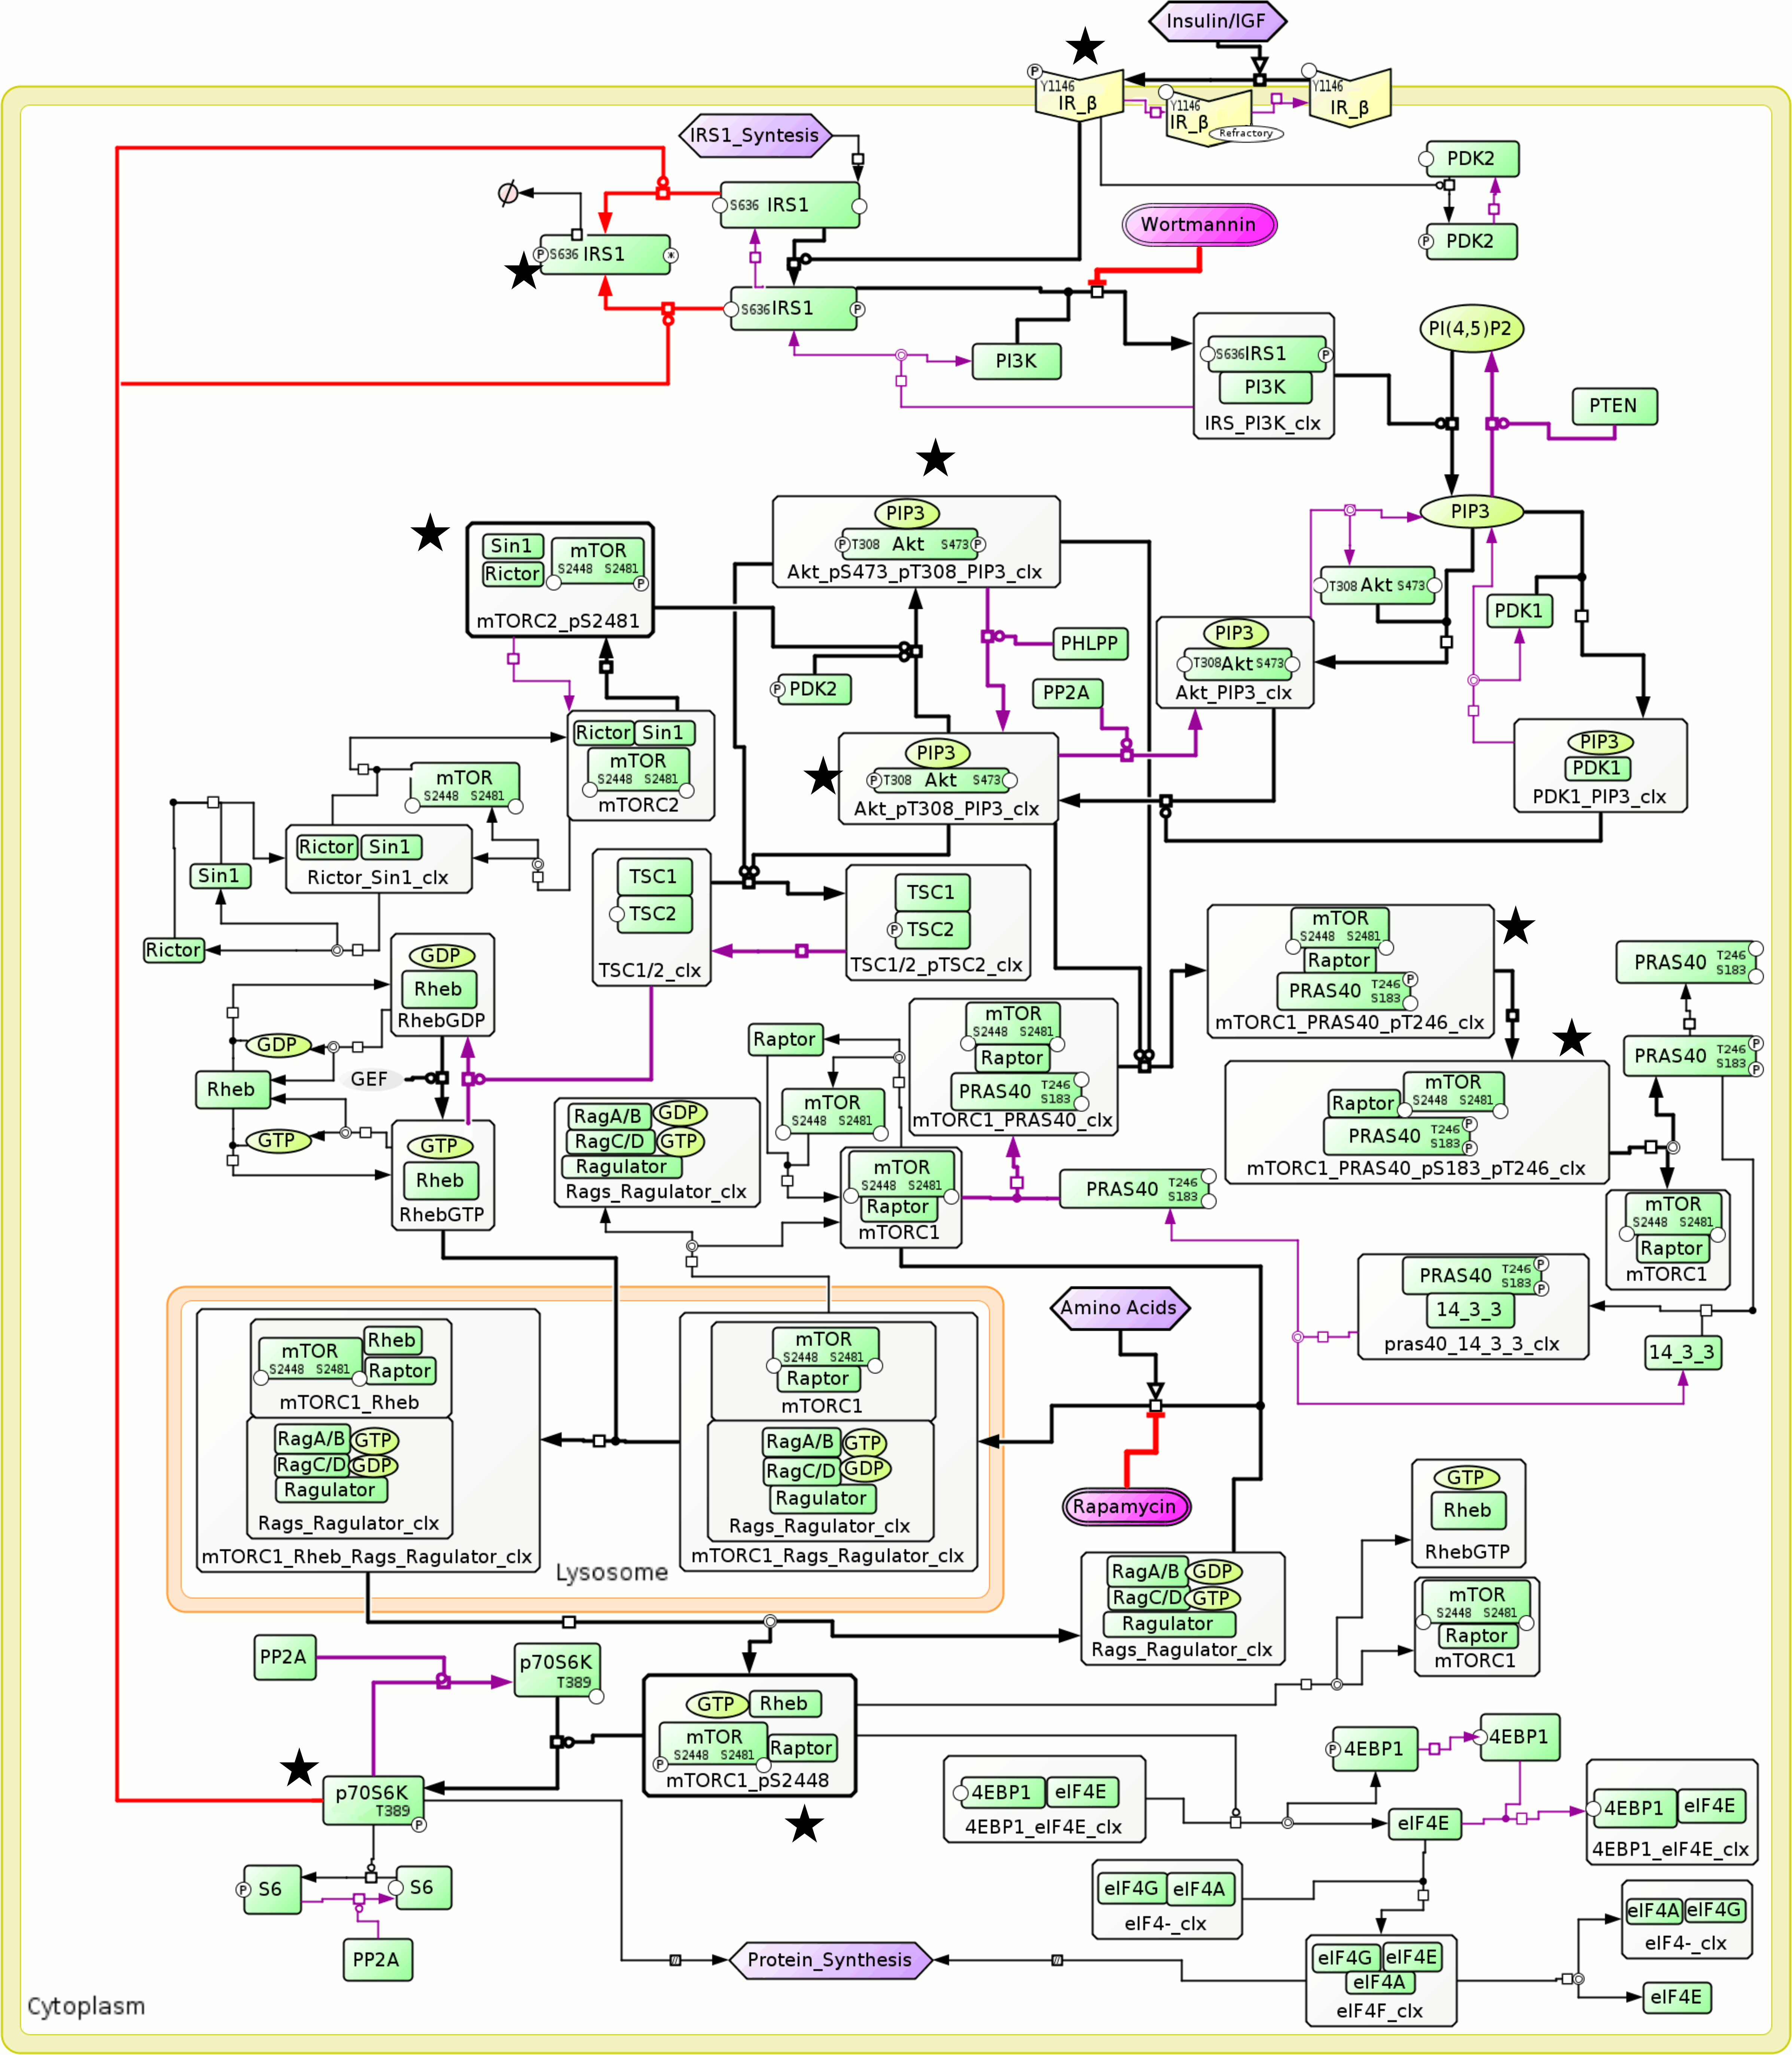
\includegraphics[width=5.7in, height=7.3in]{2002469_supp_fig1_improved.png}
		\caption[Extended graphical model of the mammalian TOR network]{A static network model of TOR signalling stimulated by amino acids plus insulin is shown in SBGN notation. This model integrates the current knowledge and guided our decision on appropriate targets for measurement. The selected targets are marked with an asterisk.}
		\label{fig:2002469_supp_fig1}
	\end{center}
\end{figure}
\clearpage

\begin{figure}[tb]
	\begin{center}
		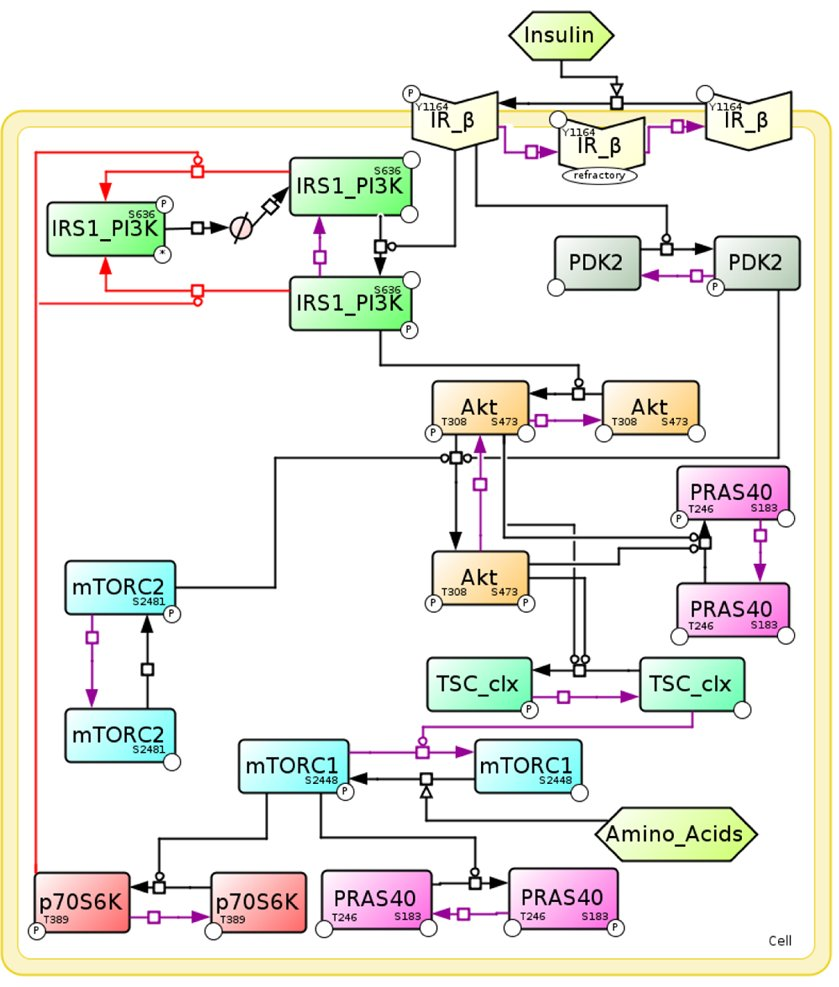
\includegraphics[scale=1.6]{2002469_fig1.jpg}
		\caption[An insulin/mTOR network graphical model]{An insulin/mTOR network graphical model. Reduced graphical model of the mTOR network activated by amino acids/insulin (see Figure \ref{fig:2002469_supp_fig1} for the extended graphical model).}
		\label{fig:2002469_fig1}
	\end{center}
\end{figure}
\clearpage

\begin{figure}[tb]
	\begin{center}
		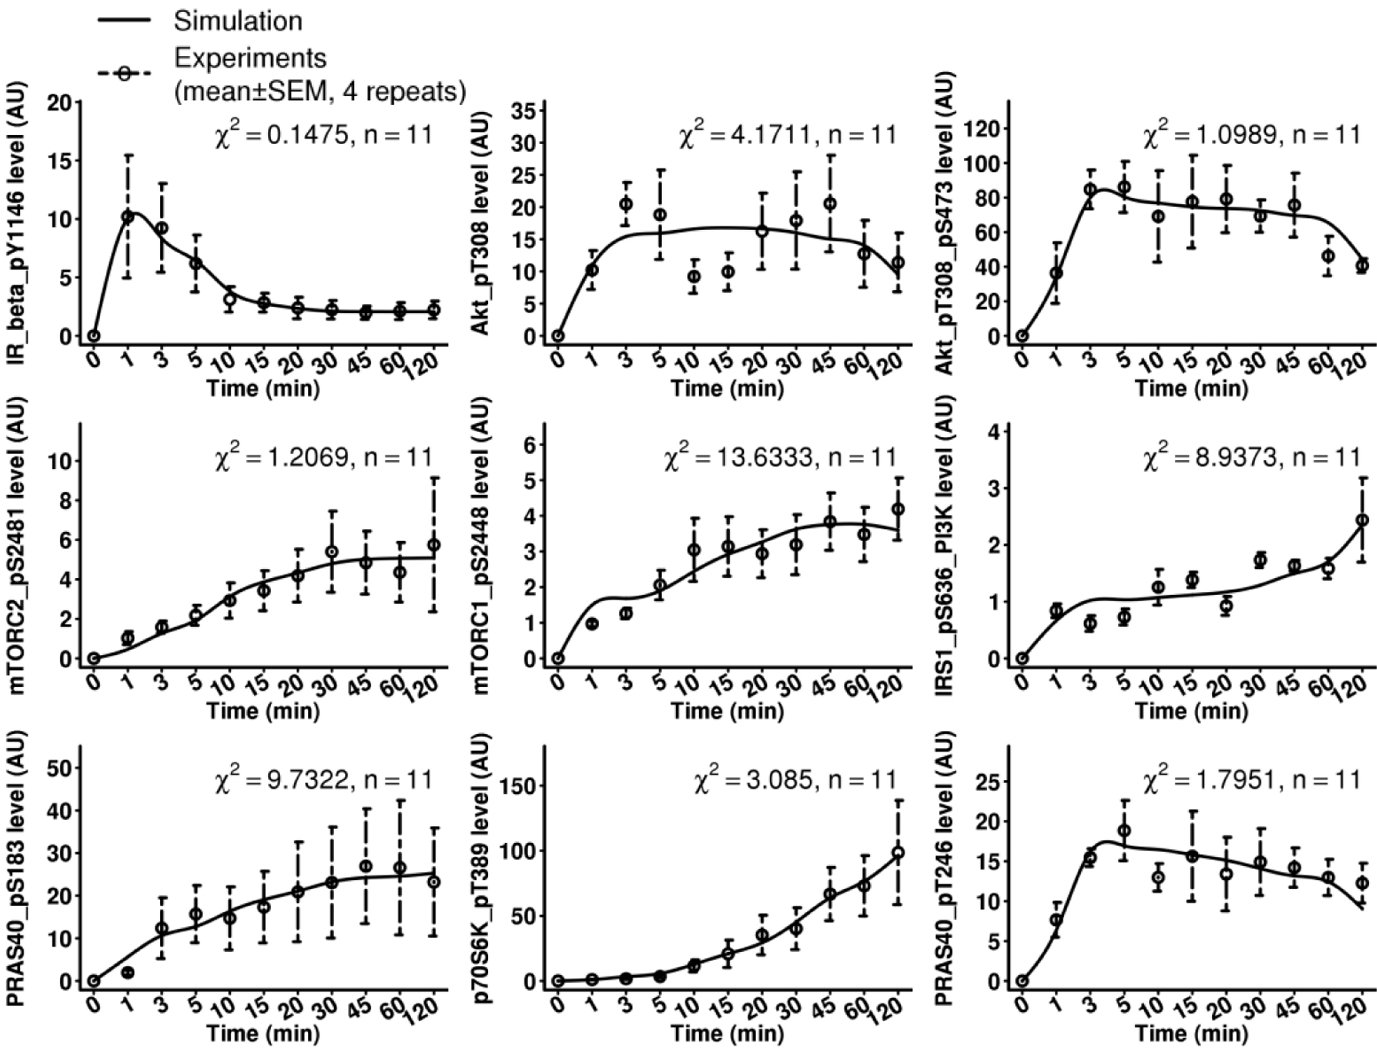
\includegraphics[scale=1.2]{2002469_fig2.jpg}
		\caption[Development of a dynamic insulin/mTOR network model]{Development of a dynamic insulin/mTOR network model. Comparison between the simulated time courses of the general model (solid lines) and the experimental time courses (points, dotted error bars) within [0, 120] min. For each curve, the $\chi^2$ computed over $n$ time points, is reported as goodness-of-fit measure. Experimental data based on quantitative immunoblotting time course by measuring phosphorylation dynamics of central network components (four replicates). \emph{In vitro} experiments were performed by Annika Sonntag, Freiburg University, Germany.}
		\label{fig:2002469_fig2}
	\end{center}
\end{figure}
\clearpage

\begin{figure}[tb]
	\begin{center}
		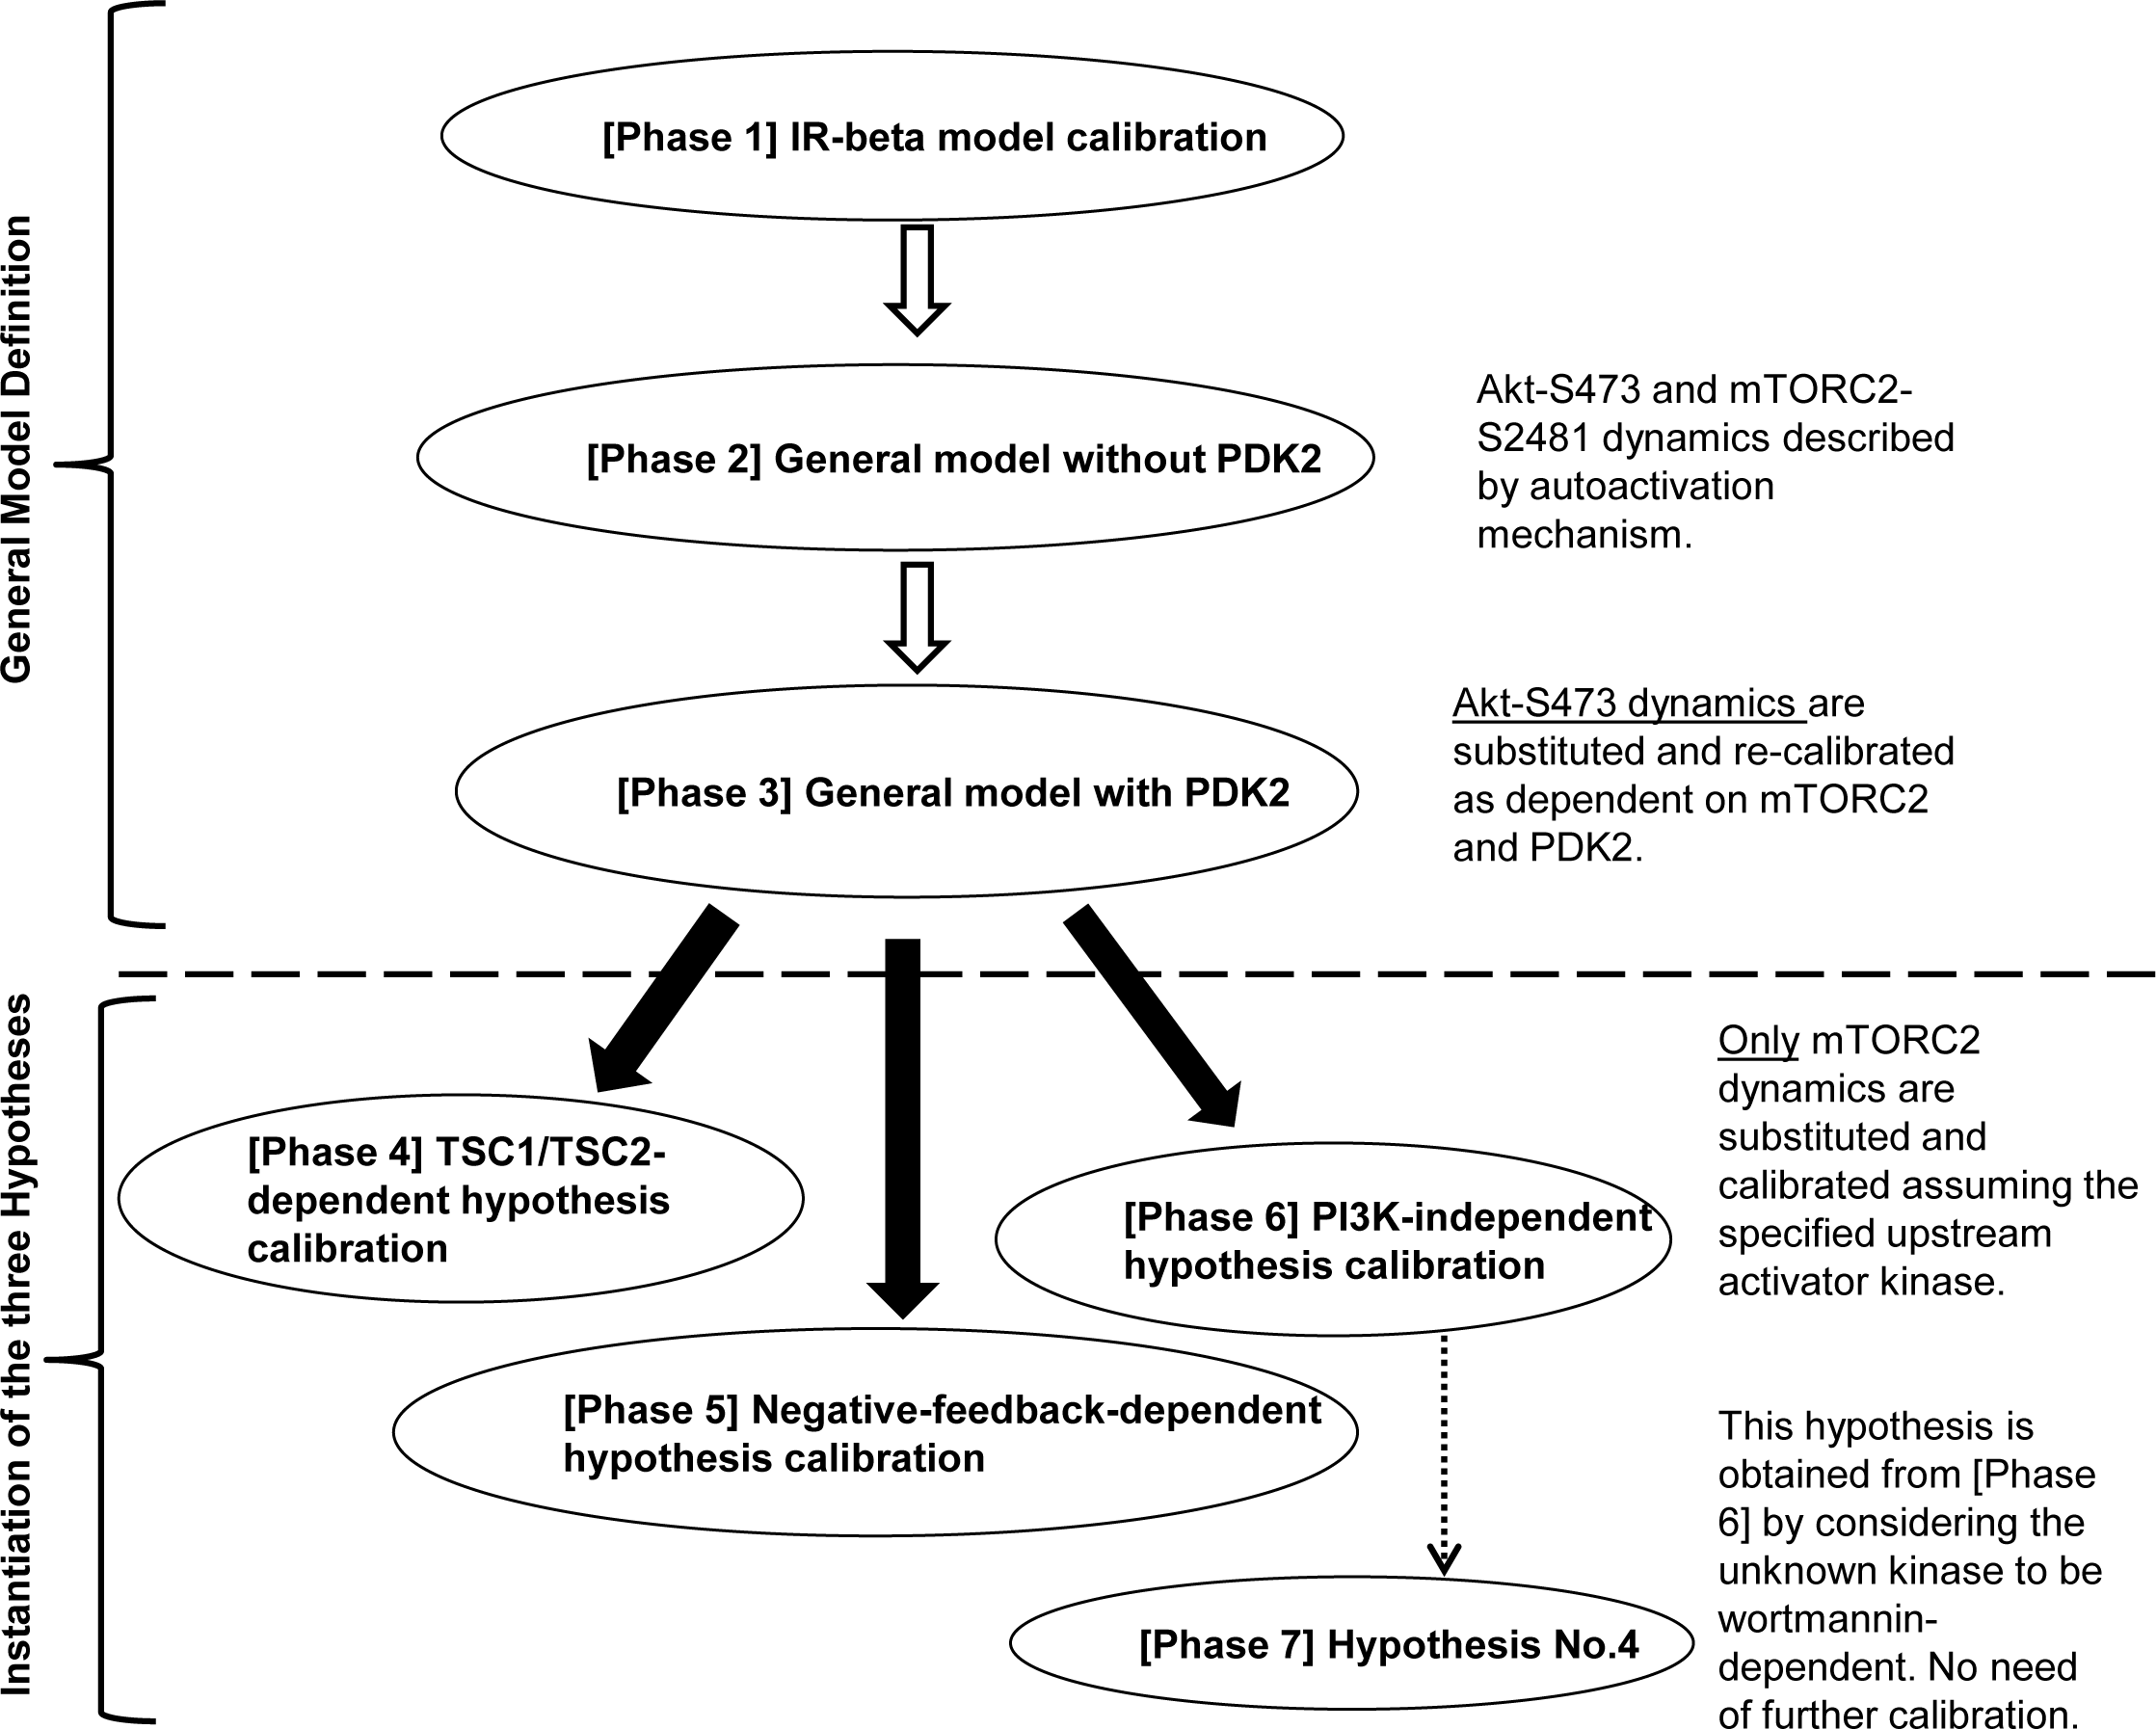
\includegraphics[scale=0.7]{2002469_supp_fig3.png}
		\caption[Phases of the calibration process]{Phases of the calibration process. The approach for defining our model was hierarchical and structured in two main parts. Part 1 (Phases 1-3) was the development of a general model without regulation of mTORC2 and Part 2 (Phases 4-7) was the introduction of specific hypotheses for regulation of mTORC2. In Phase 1, the kinetic rate constants of the insulin receptor were calibrated independently because the insulin receptor module was not regulated by the rest of the network. In Phase 2, the kinetic rate constants for the model representing the entire network without PDK2 were calibrated, assuming that the phosphorylation dynamics of mTOR-S2481 and Akt-S473 dynamics were regulated by autoactivation. In Phase 3, PDK2 was added to the network and the autoregulation mechanism controlling phosphorylation of Akt-S473 was replaced with the regulation by both mTORC2 and PDK2. Part 2 (Phases 4-7) of the calibration process concerned the introduction of the three hypotheses 
(Hypothesis 1,2, and 3) for mTORC2 activation from the general model defined in Part 1 (Phase 3). The development and calibration of these hypotheses only required substitution of the mTORC2 dynamics of the general model with the specific regulation of the corresponding hypothesis and then recalibration of these new kinetic parameters. In Phase 7, Hypothesis 4 was obtained from the PI3K-independent model by transforming the unknown kinase into one dependent on Wortmannin, which did not involve further calibration.}
		\label{fig:2002469_supp_fig3}
	\end{center}
\end{figure}
\clearpage

\begin{figure}[tb]
	\begin{center}
		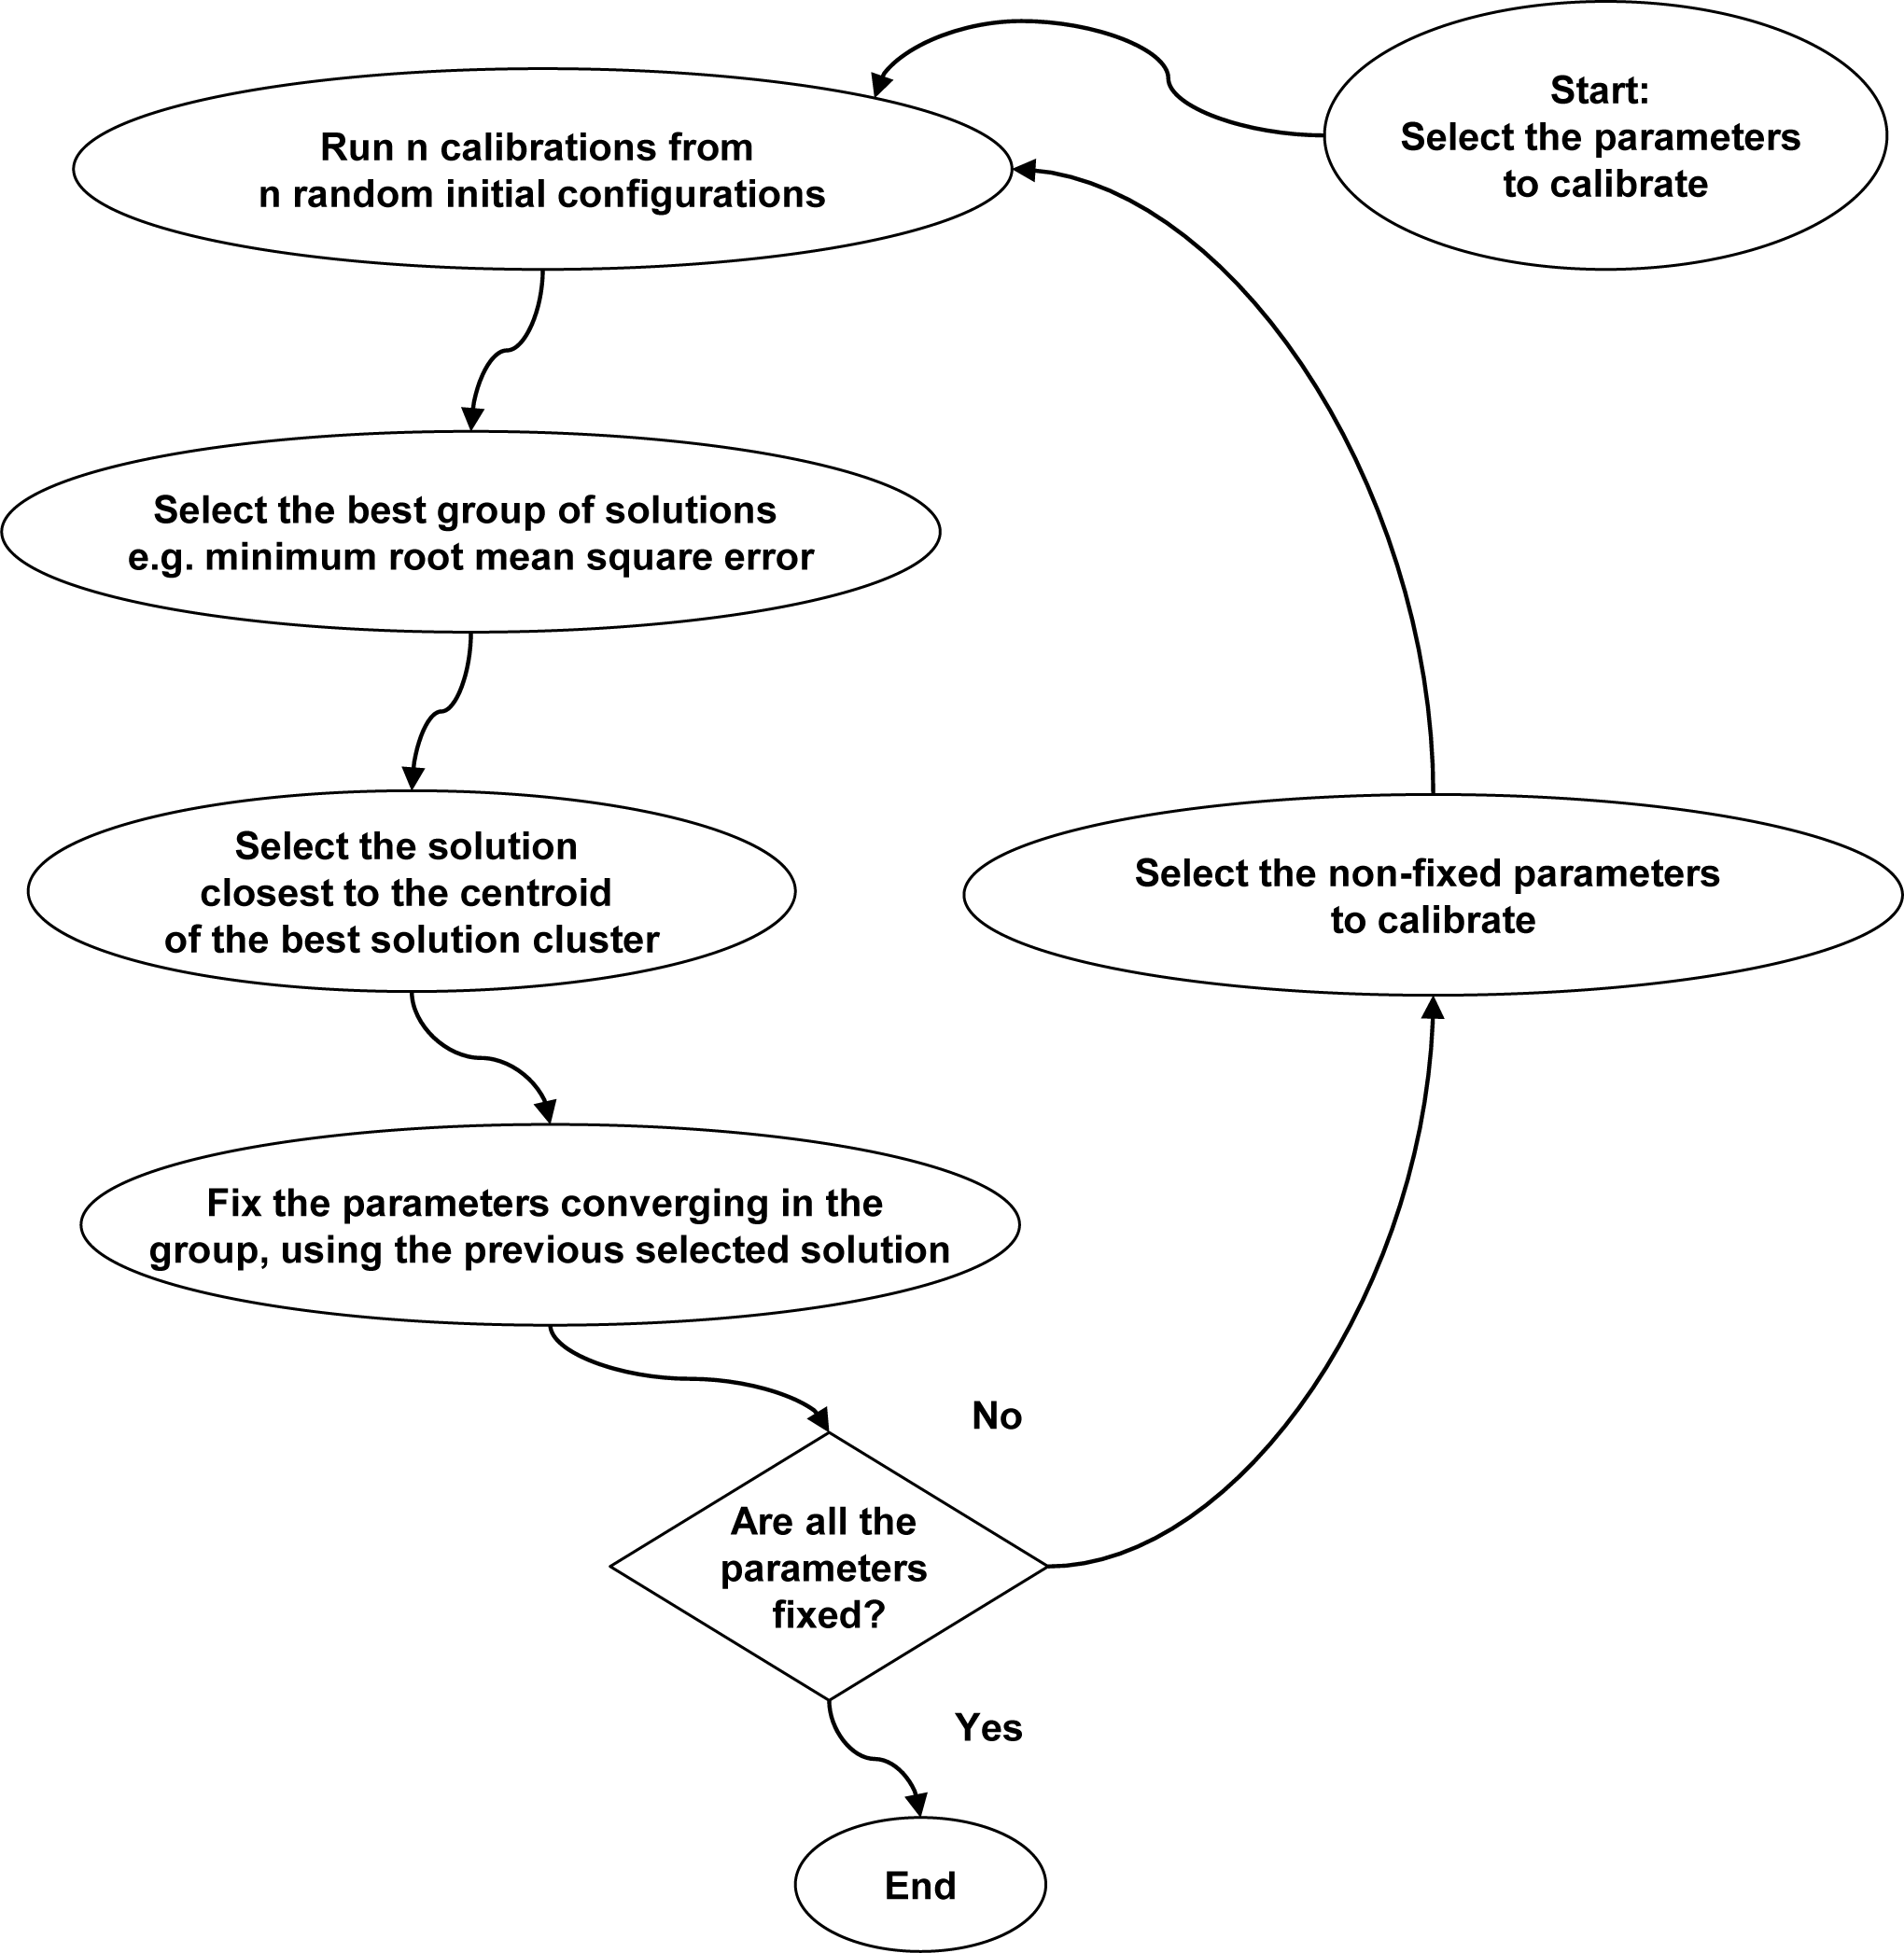
\includegraphics[scale=0.7]{2002469_supp_fig4.png}
		\caption[Detail of a calibration phase]{Detail of a calibration phase. The flow chart shows the details of the parameter calibration procedure. The procedure began with the selection of the set of parameters to estimate. After completing the calibrations, the procedure selected the subset of the solutions that obtained the minimum root mean square error (best solutions). The closest solution to the centroid of the best solution cluster was selected and the values common to all the solutions were fixed. All the parameters that were not fixed were selected for the next step of calibration. The procedure terminated when there were no further parameters to calibrate. In the model calibration, all the parameters were identified in only one iteration step.}
		\label{fig:2002469_supp_fig4}
	\end{center}
\end{figure}
\clearpage

\begin{figure}[tb]
	\begin{center}
		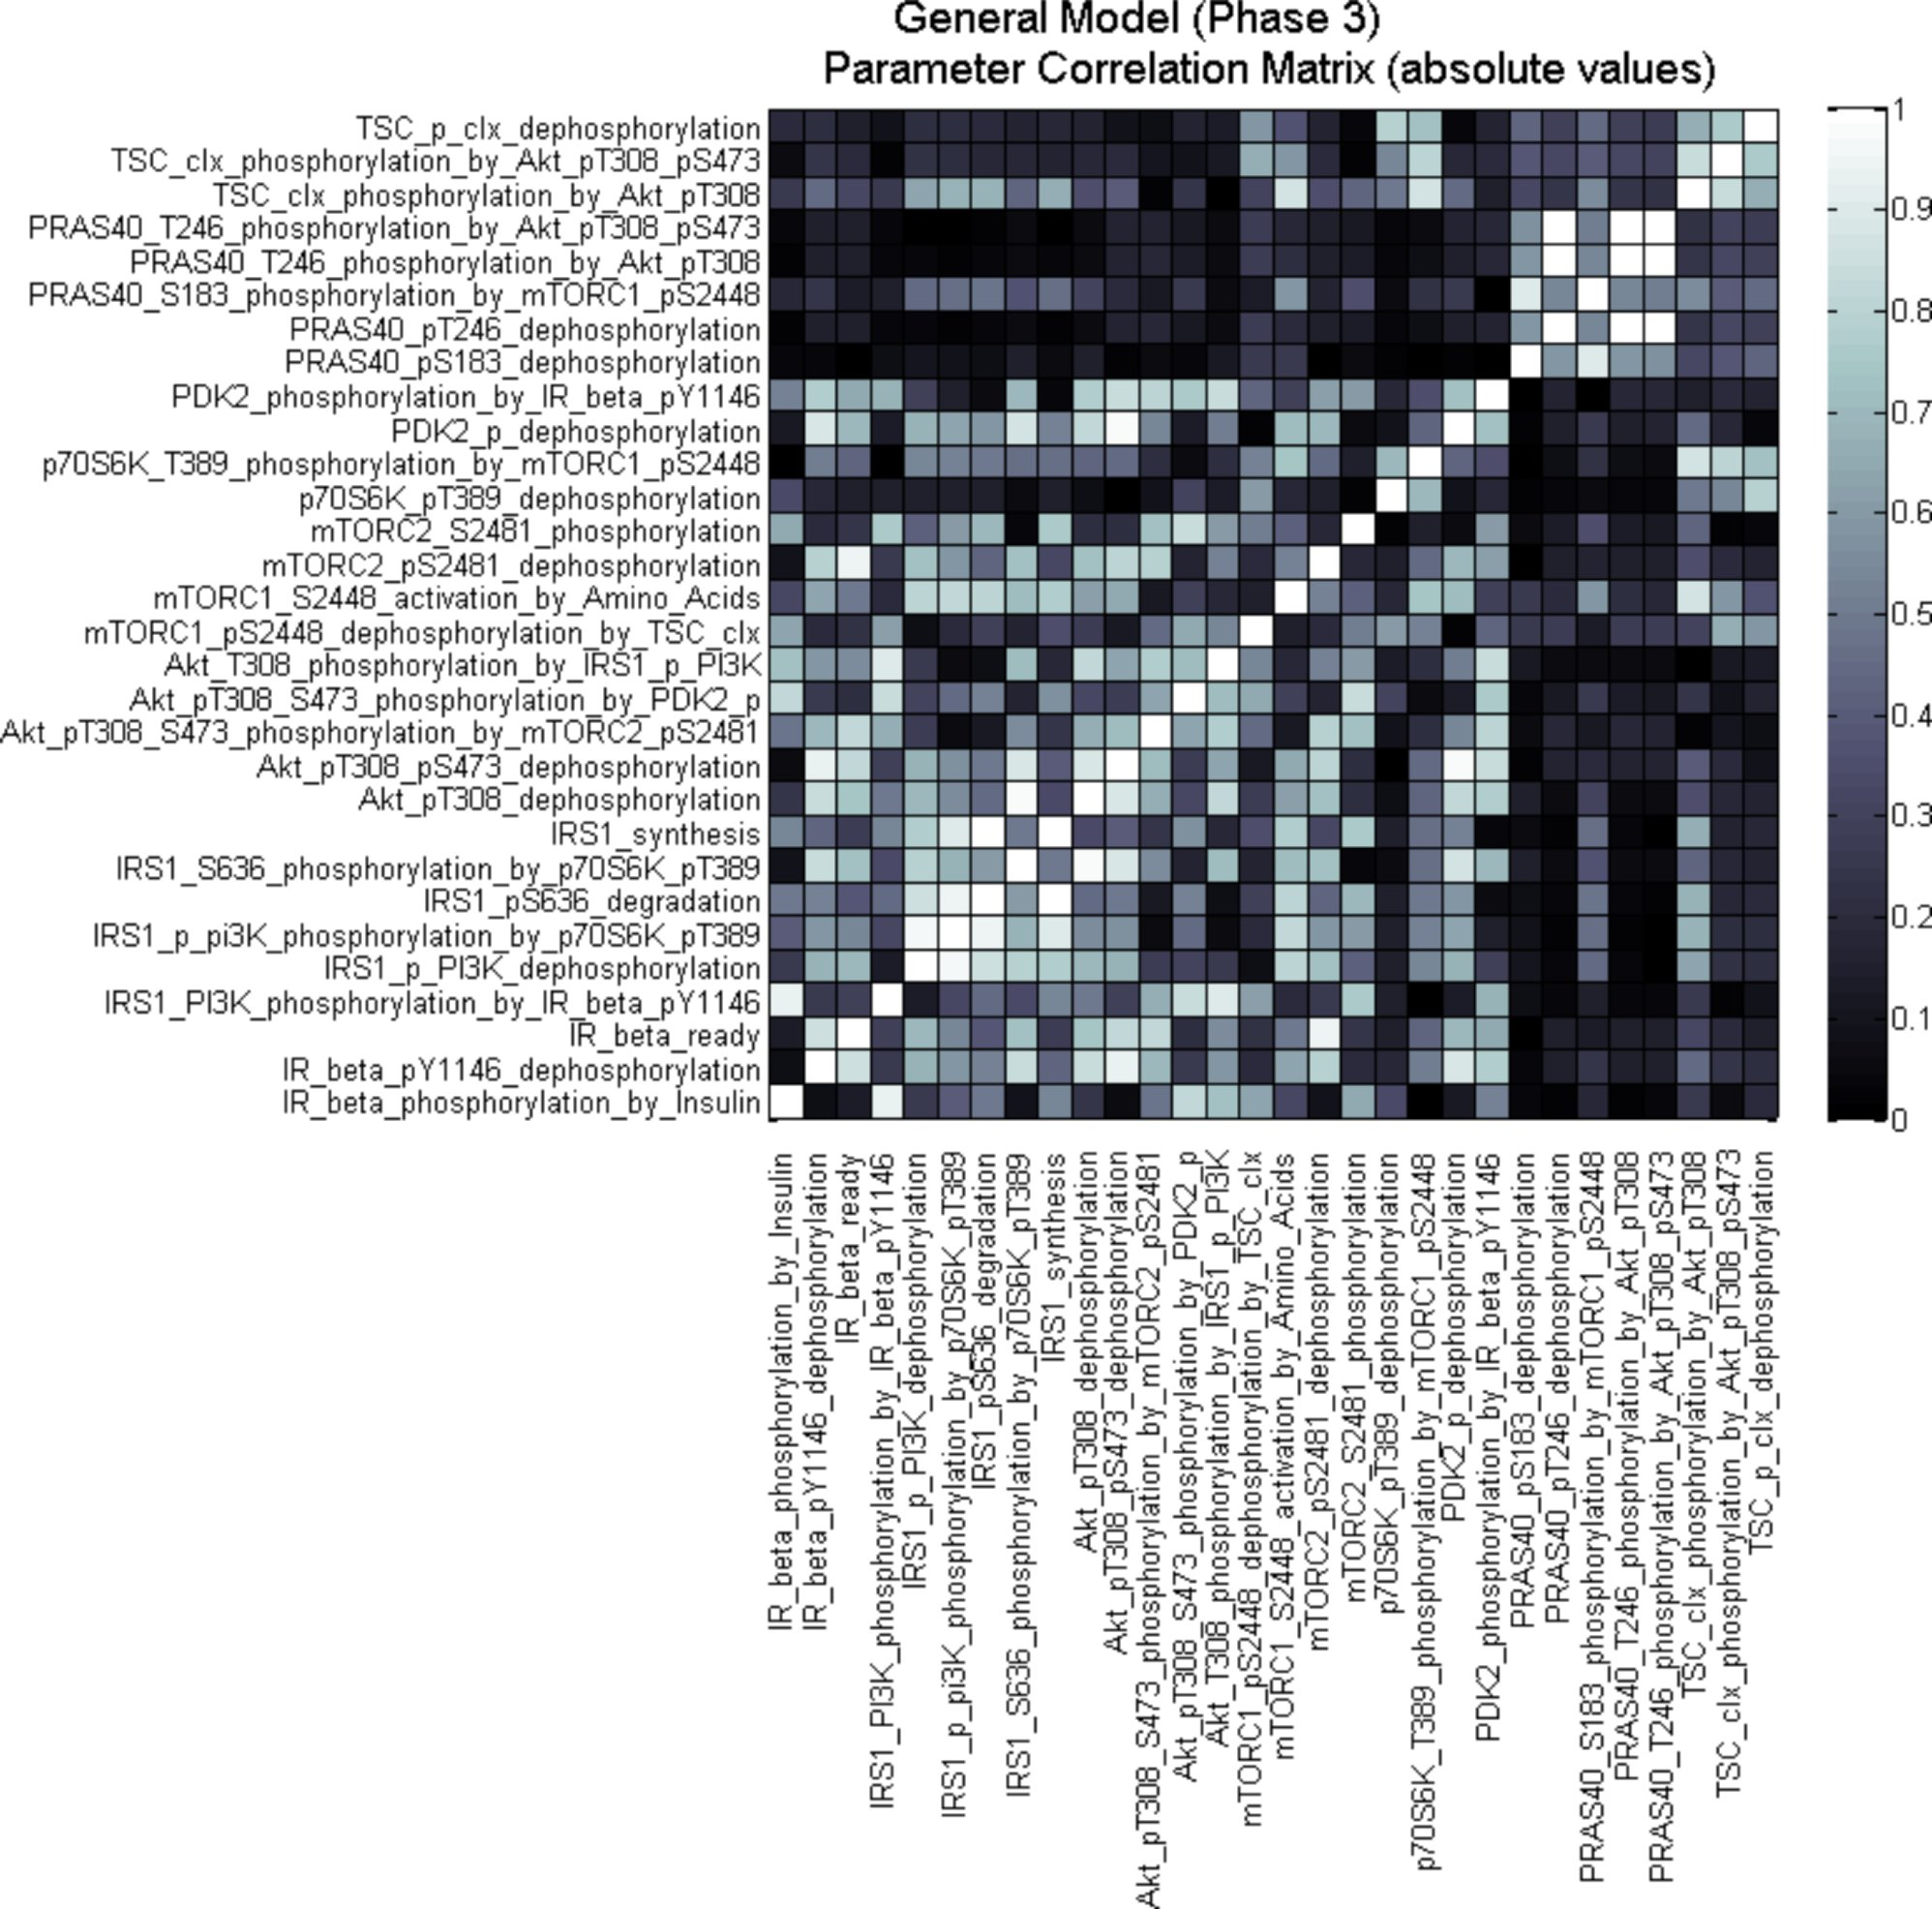
\includegraphics[scale=0.8]{2002469_supp_fig5.jpg}
		\caption[Identifiability analysis for the general model]{Identifiability analysis for the general model. Parameter identifiability is based on sensitivity analysis and parameter correlation as computed by SBPD Matlab Toolbox. The symmetric matrix shows the parameter correlation in absolute values. High parameter correlations suggest potential issues in identifying the corresponding parameters independently (the elements on the diagonal obviously have correlation equal to 1). Conversely, low parameter correlations indicate that the corresponding parameters can be identified independently. Our experimental data were used in computing the reported identifiability analysis.}
		\label{fig:2002469_supp_fig5}
	\end{center}
\end{figure}
\clearpage

\begin{figure}[tb]
	\begin{center}
		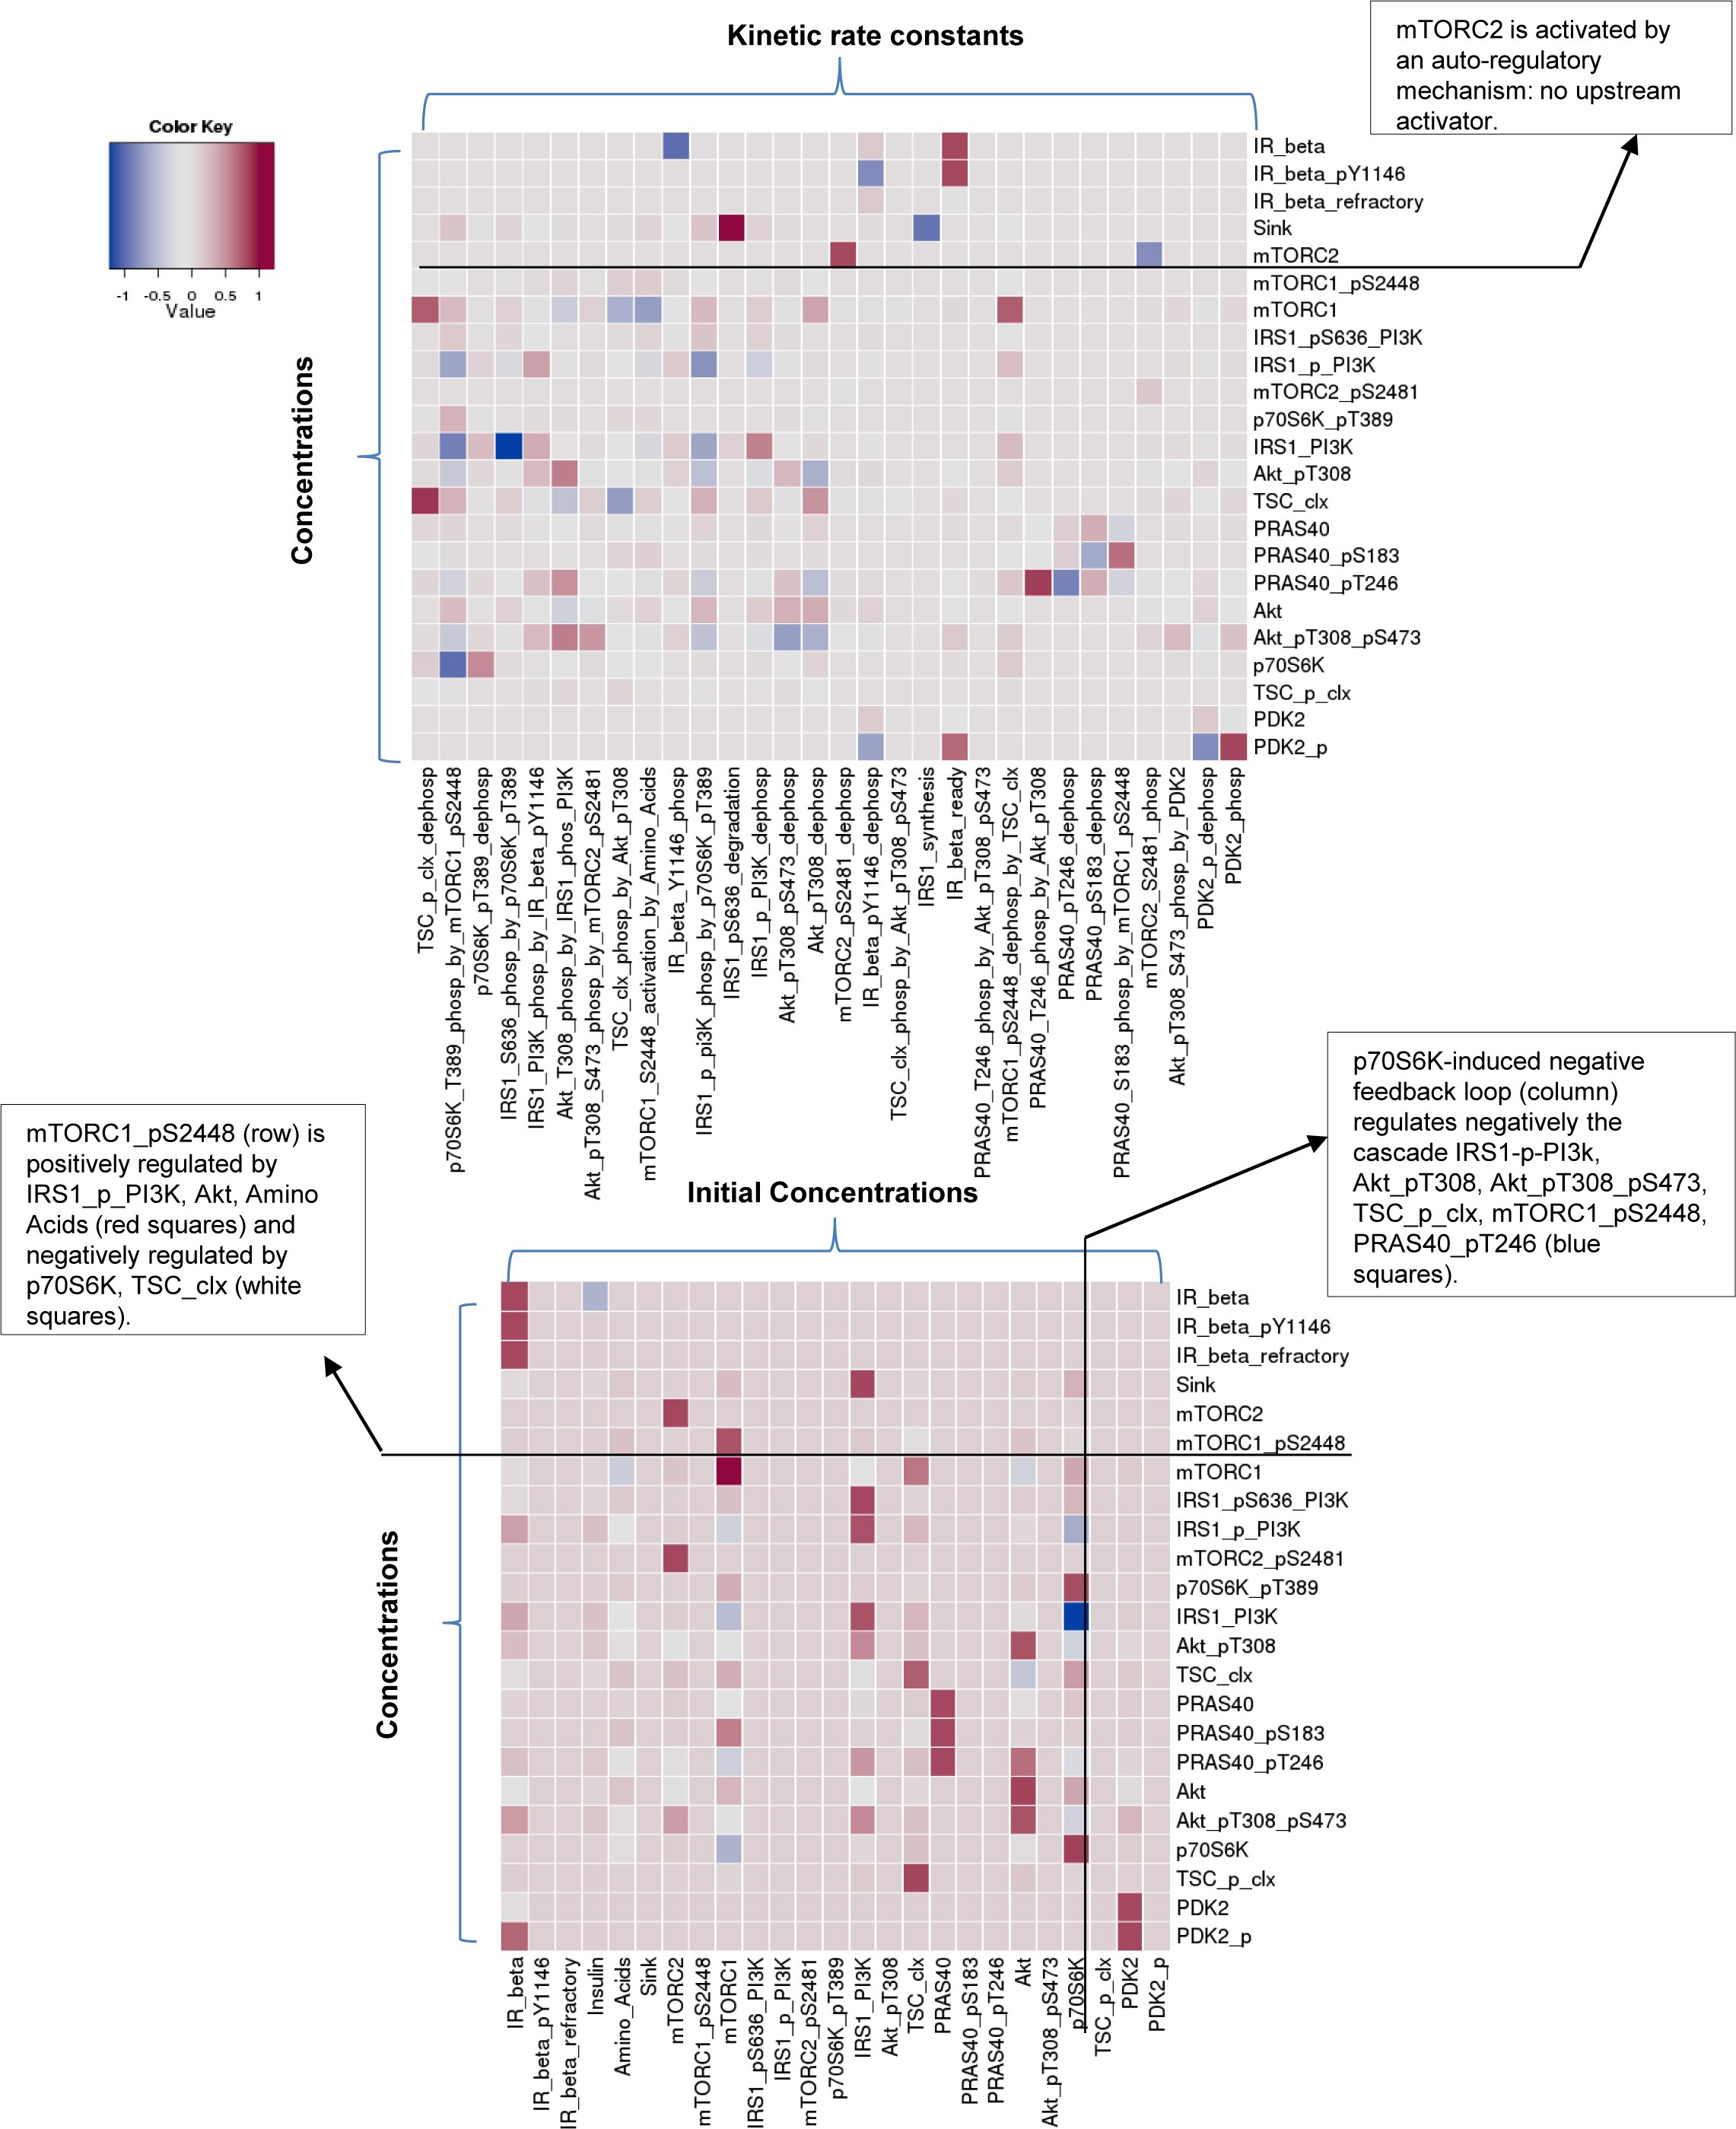
\includegraphics[width=5.60in]{2002469_supp_fig6.jpg}
		\caption[Sensitivity analysis for the general model]{Sensitivity analysis for the general model. The top plot illustrates the sensitivity analysis of the model by row, in response to the perturbations of the kinetic rates constants shown in columns. The bottom plot shows the model sensitivity analysis of the initial concentrations of the modelled species by row with perturbations shown in columns. Values were normalised in the range [-1, 1]. Positive values (red squares) represent positive regulation; negative ones (white-blue squares) represent inhibition.}
		\label{fig:2002469_supp_fig6}
	\end{center}
\end{figure}
\clearpage

\begin{figure}[tb]
	\begin{center}
		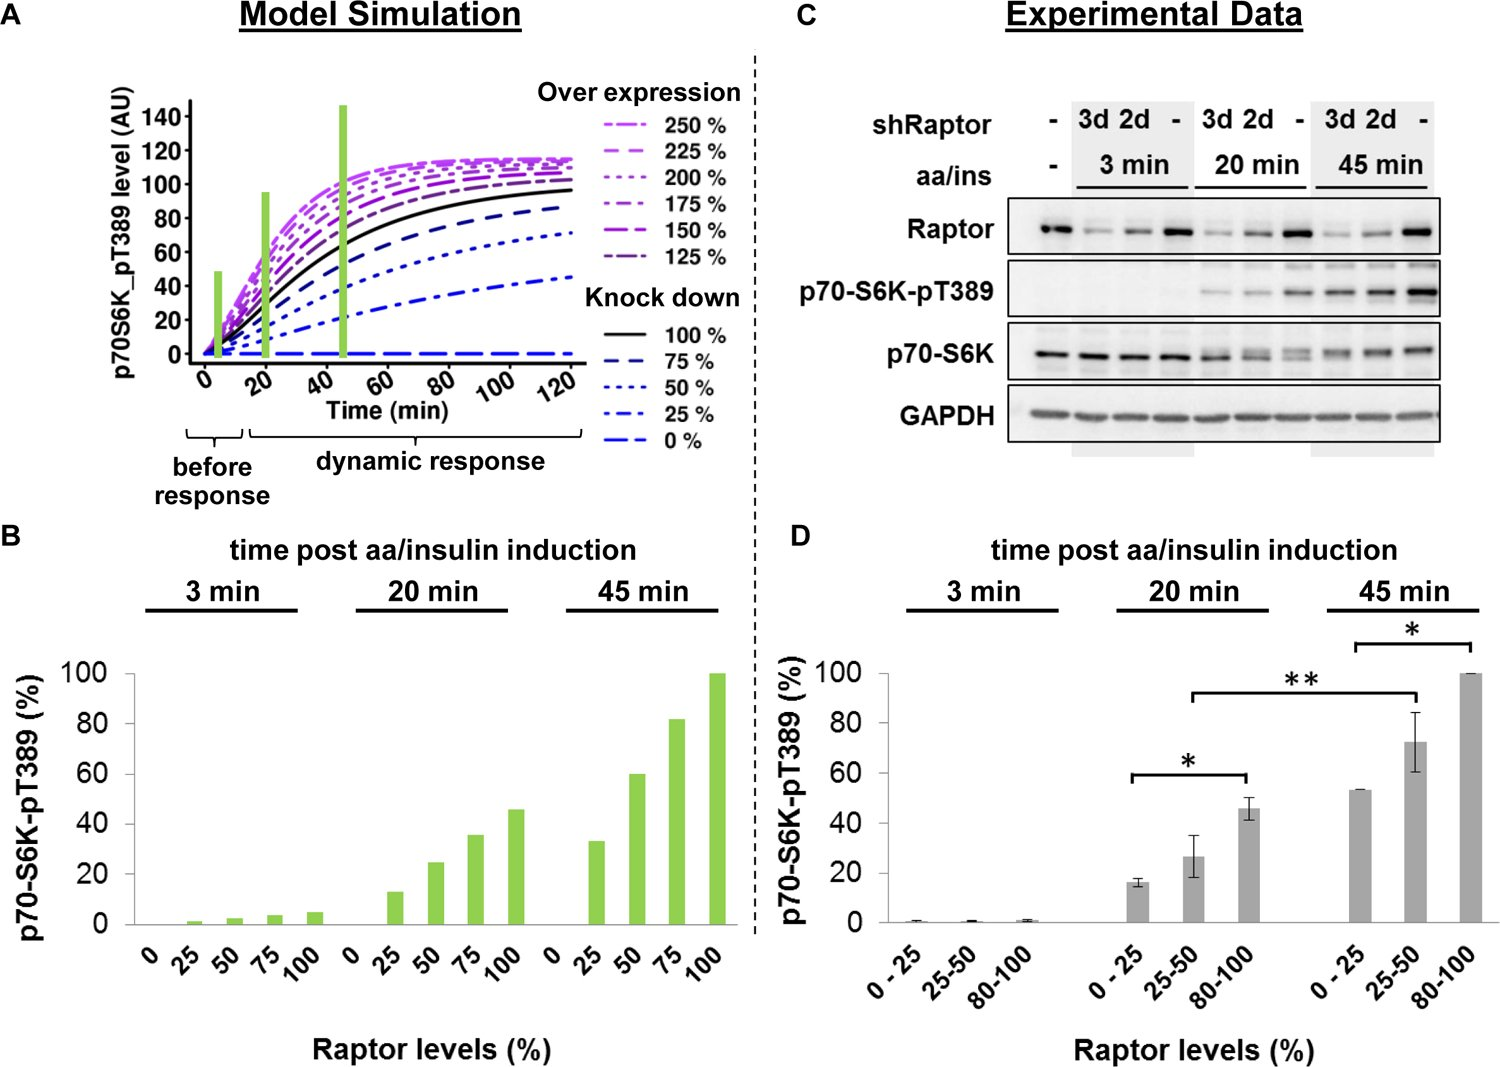
\includegraphics[scale=1.05]{2002469_fig3.jpg}
		\caption[Validation: dynamic response of p70-S6K-pT389 to gradual Raptor inhibition]{Validation: dynamic response of p70-S6K-pT389 to gradual Raptor inhibition. (A) Model predictions for p70-S6K-pT389 dynamics in response to a perturbation of mTORC1. The curves show the simulated response to gradual mTORC1 inhibition starting at 5-10 minutes after induction with amino acids/insulin. The model was simulated with both mTORC1 overexpression and knockdown conditions. Time points for experimental validation are indicated by green lines. (B) Simulated and quantified relative amounts of p70-S6K-pT389 under conditions of mTORC1 reduction (0, 25, 50, 75, 100 \%) at selected time points after induction with amino acids/insulin. (C) Experimental validation of the effect of gradual Raptor knockdown (shRaptor) on p70-S6K phosphorylation in starved cells induced with amino acids/ins for the indicated times. Data are representative of 3 experiments. d = days. (D) Experimentally determined and quantified p70-S6K-pT389 
amounts at the indicated times after induction with amino acids/insulin in cells in which Raptor was knocked down. Data are the average and SEM of 3 experiments. * $P\;<\;0.05$, ** $P\;<\;0.01$; low Raptor levels compared to high Raptor levels after 20 min and 45 min induction, 20 min compared to 45 min induction.  Differences in p70-S6K-pT389 were significant. \emph{In vitro} experiments were performed by Annika Sonntag, Freiburg University, Germany.}
		\label{fig:2002469_fig3}
	\end{center}
\end{figure}
\clearpage

\begin{figure}[tb]
	\begin{center}
		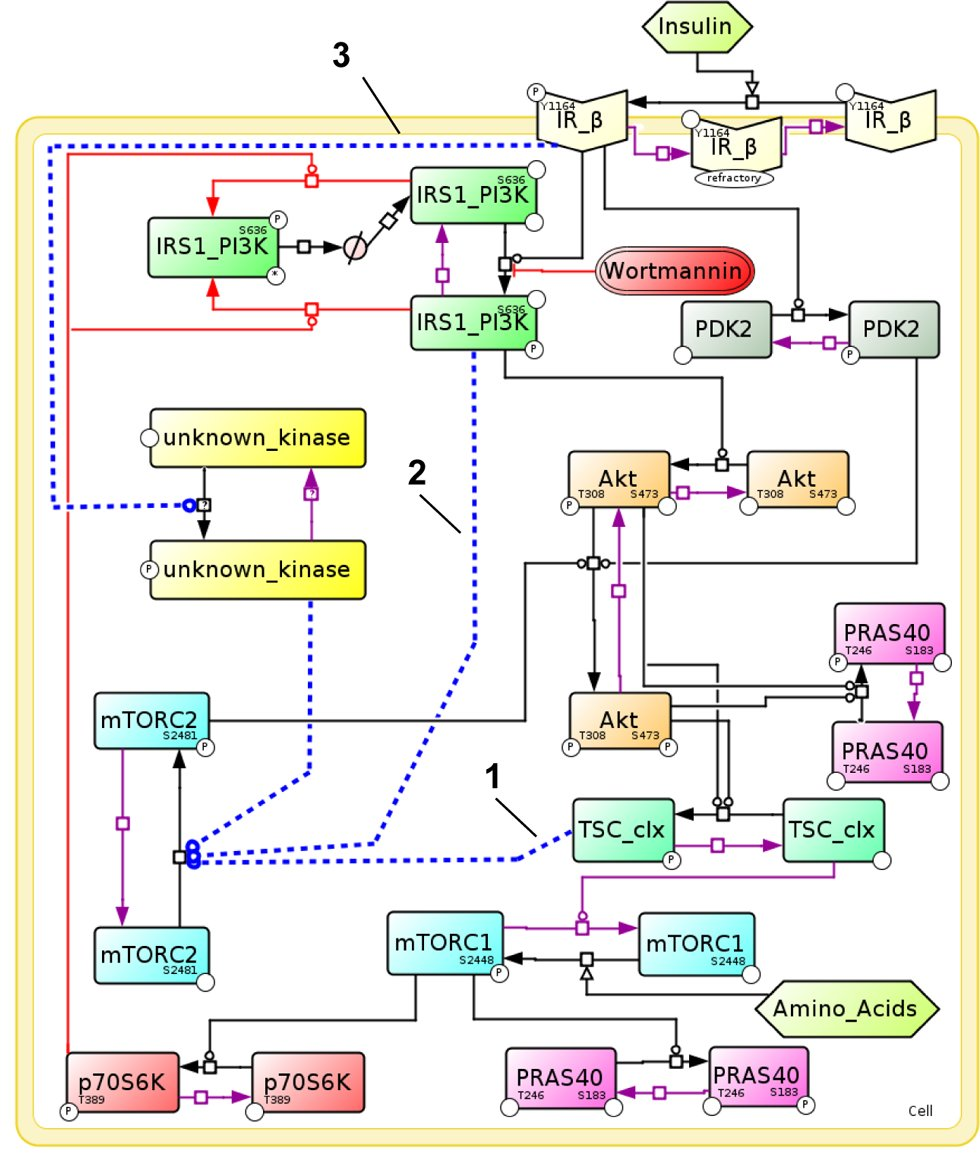
\includegraphics[scale=1.4]{2002469_fig4B.jpg}
		\caption[Three different hypotheses on mTORC2 regulation by insulin (graphical model)]{Three different hypotheses on mTORC2 regulation by insulin (graphical model). Reduced graphical network model including the three hypotheses (1, 2, 3, indicated by the dotted lines), translated into different network structures.}
		\label{fig:2002469_fig4B}
	\end{center}
\end{figure}
\clearpage

\begin{figure}[tb]
	\begin{center}
		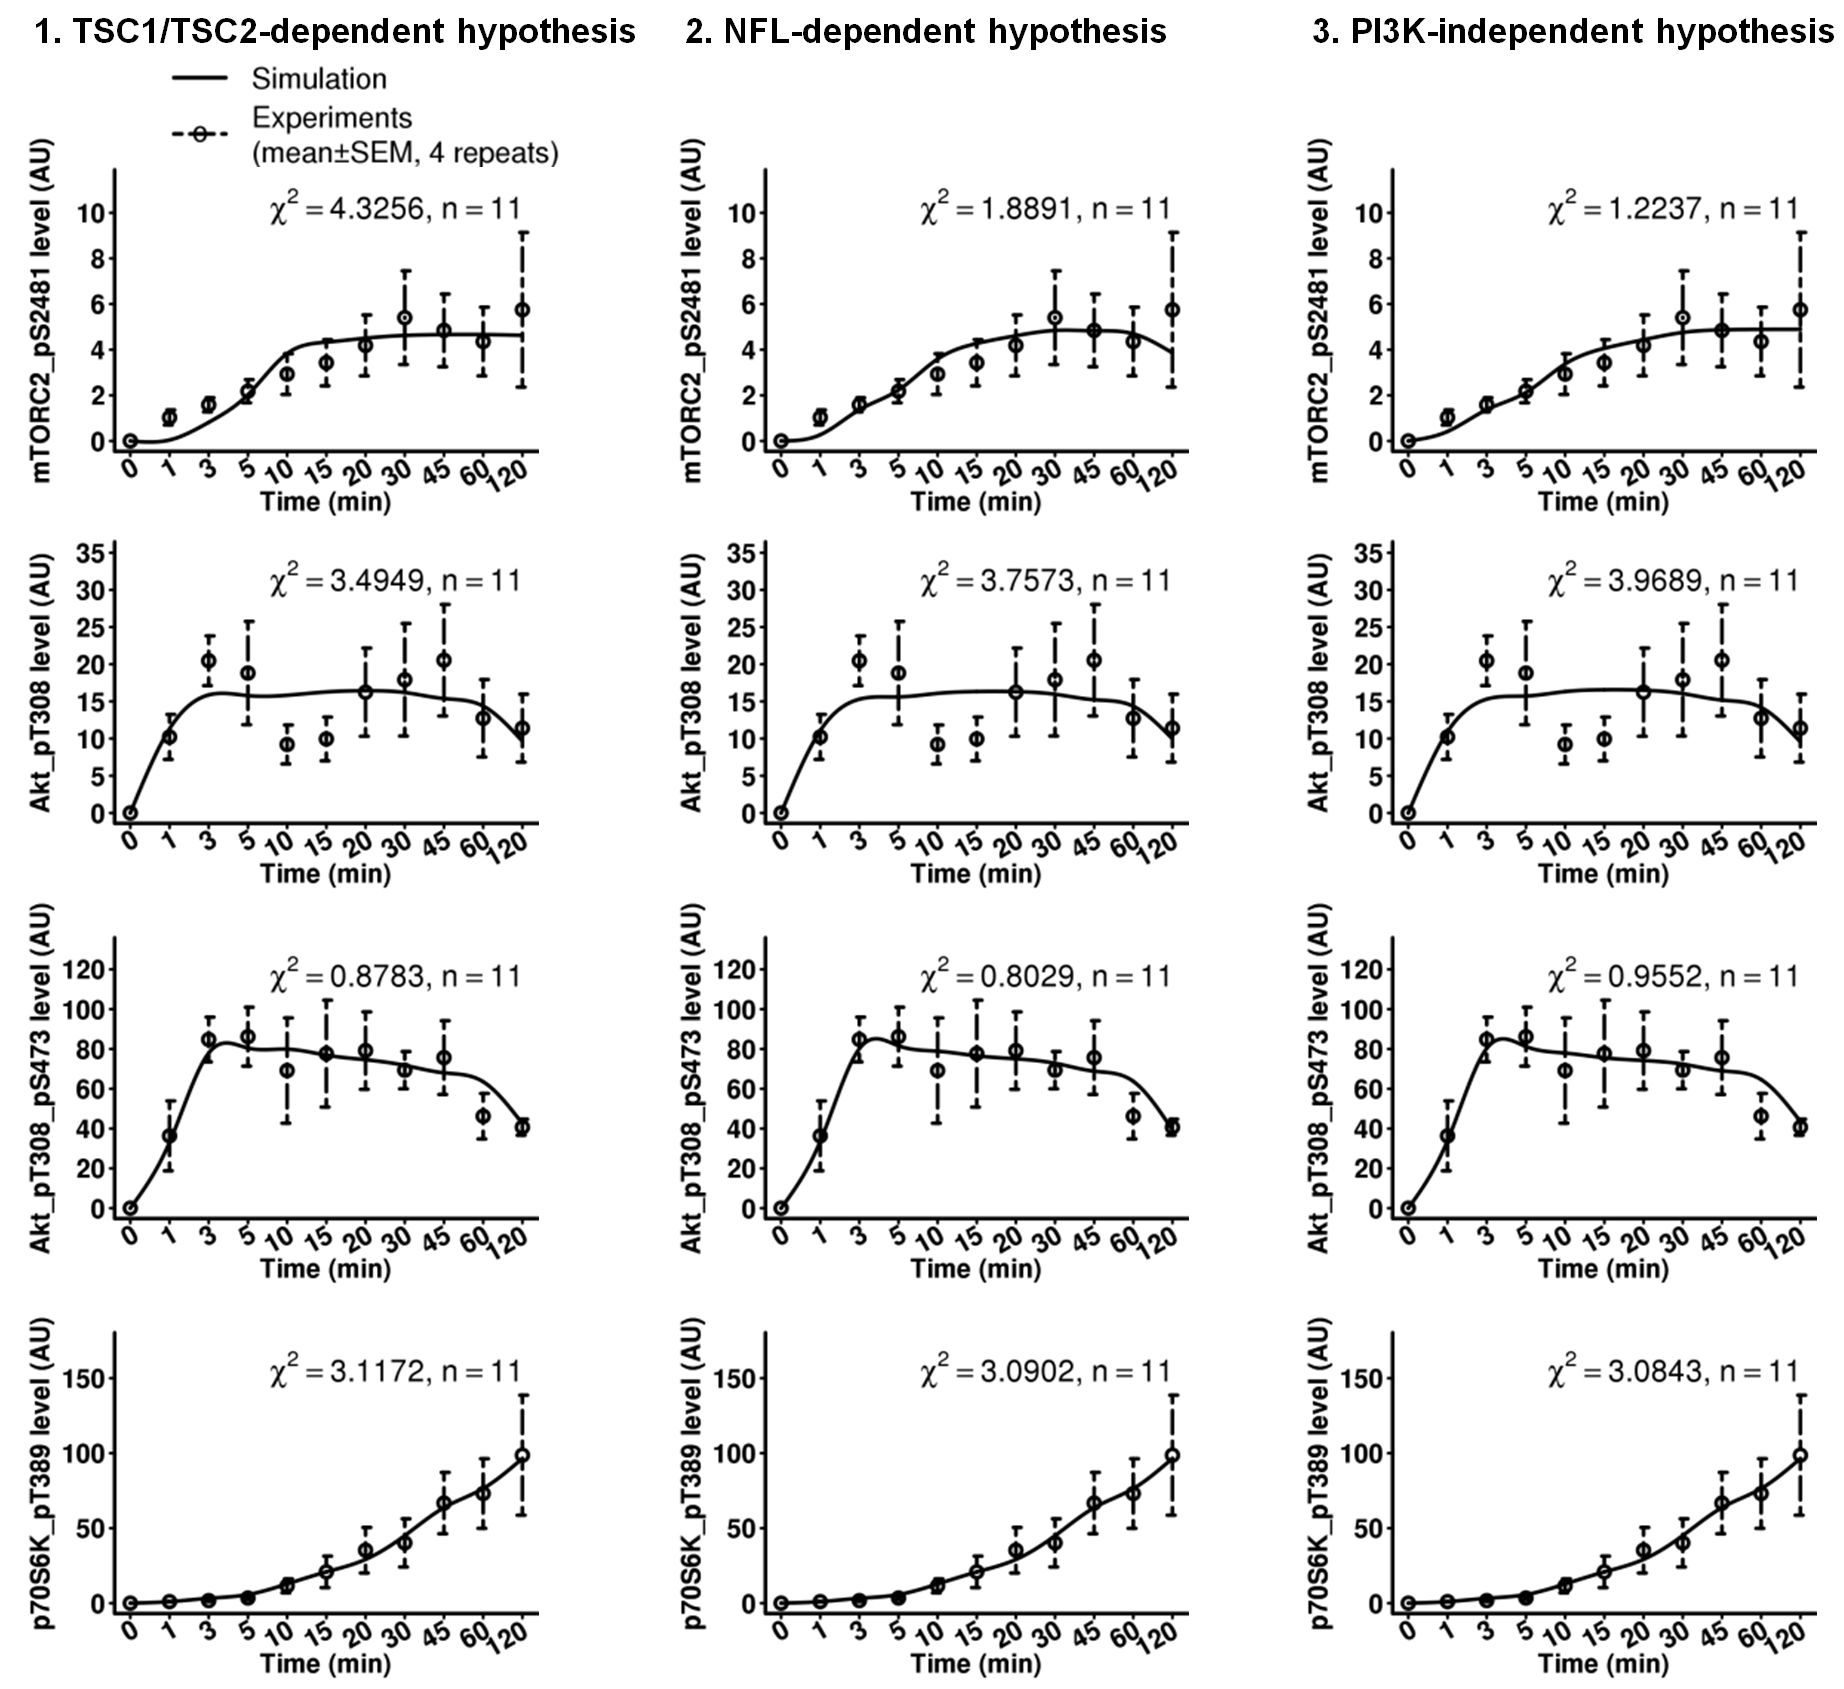
\includegraphics[scale=0.8]{2002469_fig4C.png}
		\caption[Three different hypotheses on mTORC2 regulation by insulin (dynamical models)]{Three different hypotheses on mTORC2 regulation by insulin (dynamical models). Comparisons of simulated time courses, calibrated for each hypothesis, with experimental data. Data shown are for mTORC2 readouts (mTOR-pS2481, Akt-pS473), the PI3K readout Akt-pT308, and the mTORC1 readout p70-S6K-pT389 (see Figure \ref{fig:2002469_supp_fig7} for curves of all other readouts). \emph{In vitro} experiments were performed by Annika Sonntag, Freiburg University, Germany.}
		\label{fig:2002469_fig4C}
	\end{center}
\end{figure}
\clearpage

\begin{figure}[tb]
	\begin{center}
		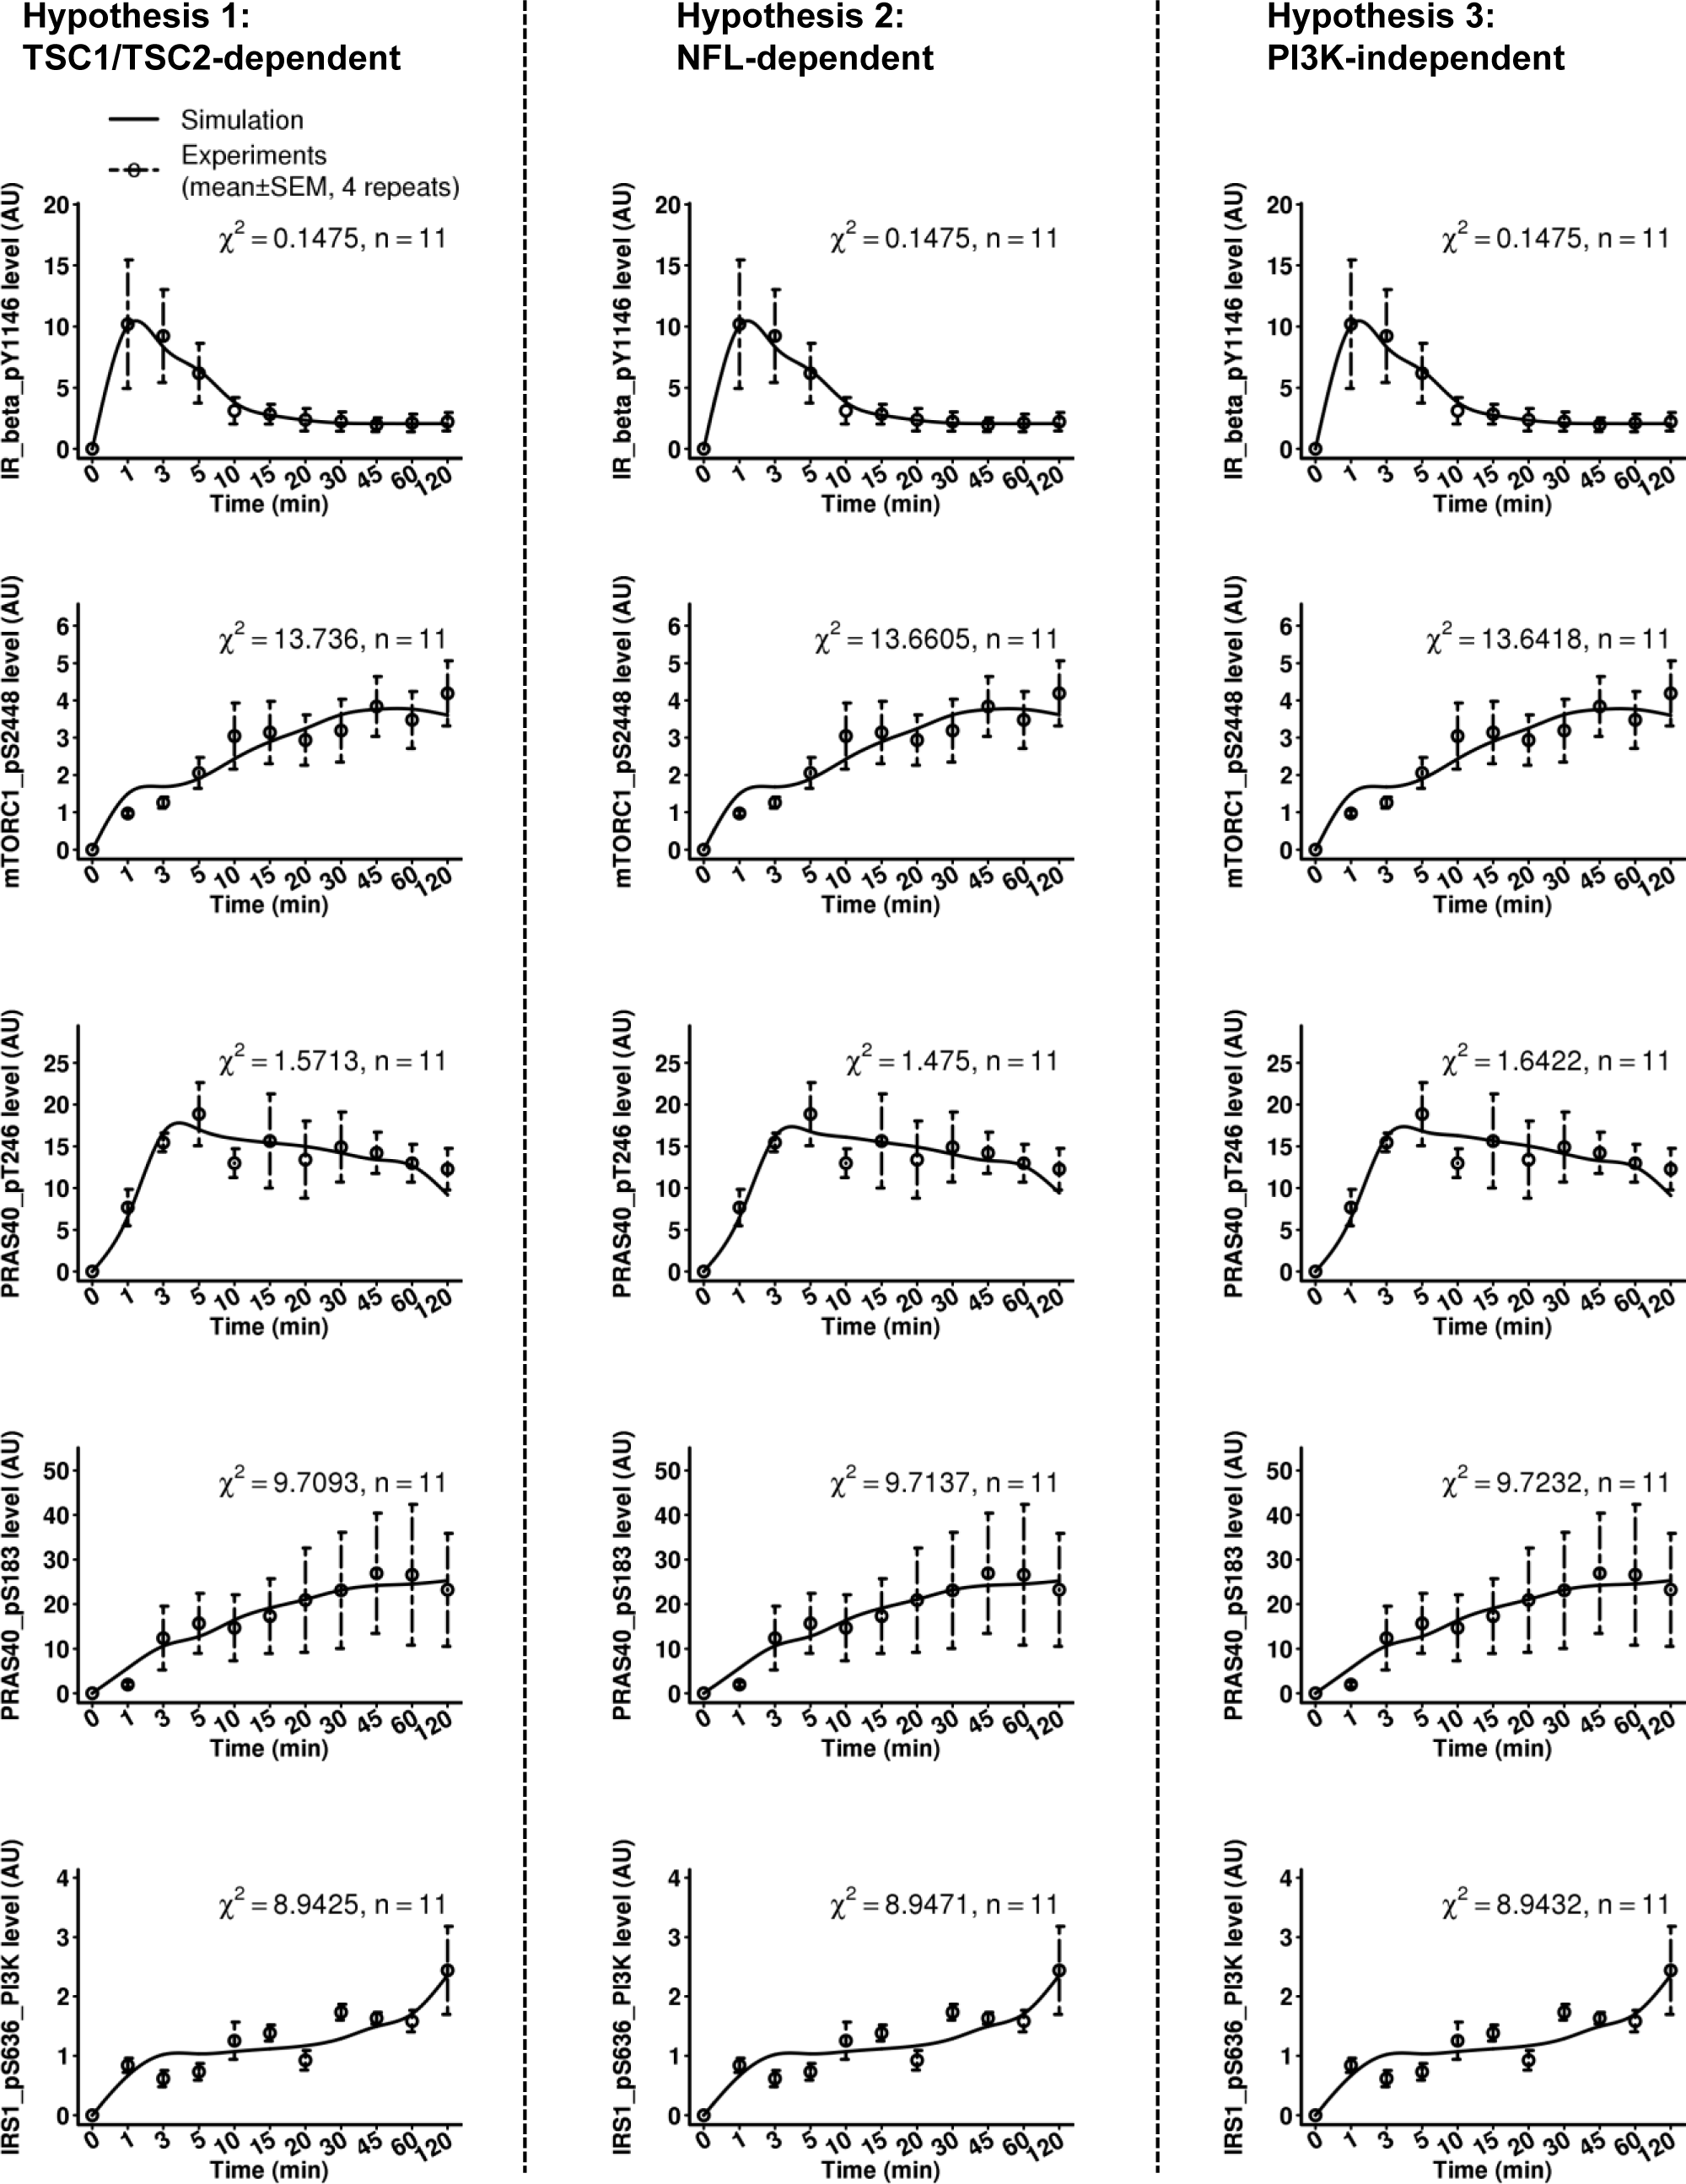
\includegraphics[scale=0.8]{2002469_supp_fig7.png}
		\caption[Comparison between the simulated and experimental time-courses for Hypotheses 1, 2, and 3 for readouts of the mTOR network]{Comparison between the simulated and experimental time-courses for Hypothesis 1, 2, and 3 for readouts of the mTOR network. The three hypotheses were consistent with each other for all the readouts indicating that introducing each hypothesis into the general model did not perturb the network. NFL = Negative Feedback Loop. \emph{In vitro} experiments were performed by Annika Sonntag, Freiburg University, Germany.}
		\label{fig:2002469_supp_fig7}
	\end{center}
\end{figure}
\clearpage

\begin{figure}[tb]
	\begin{center}
		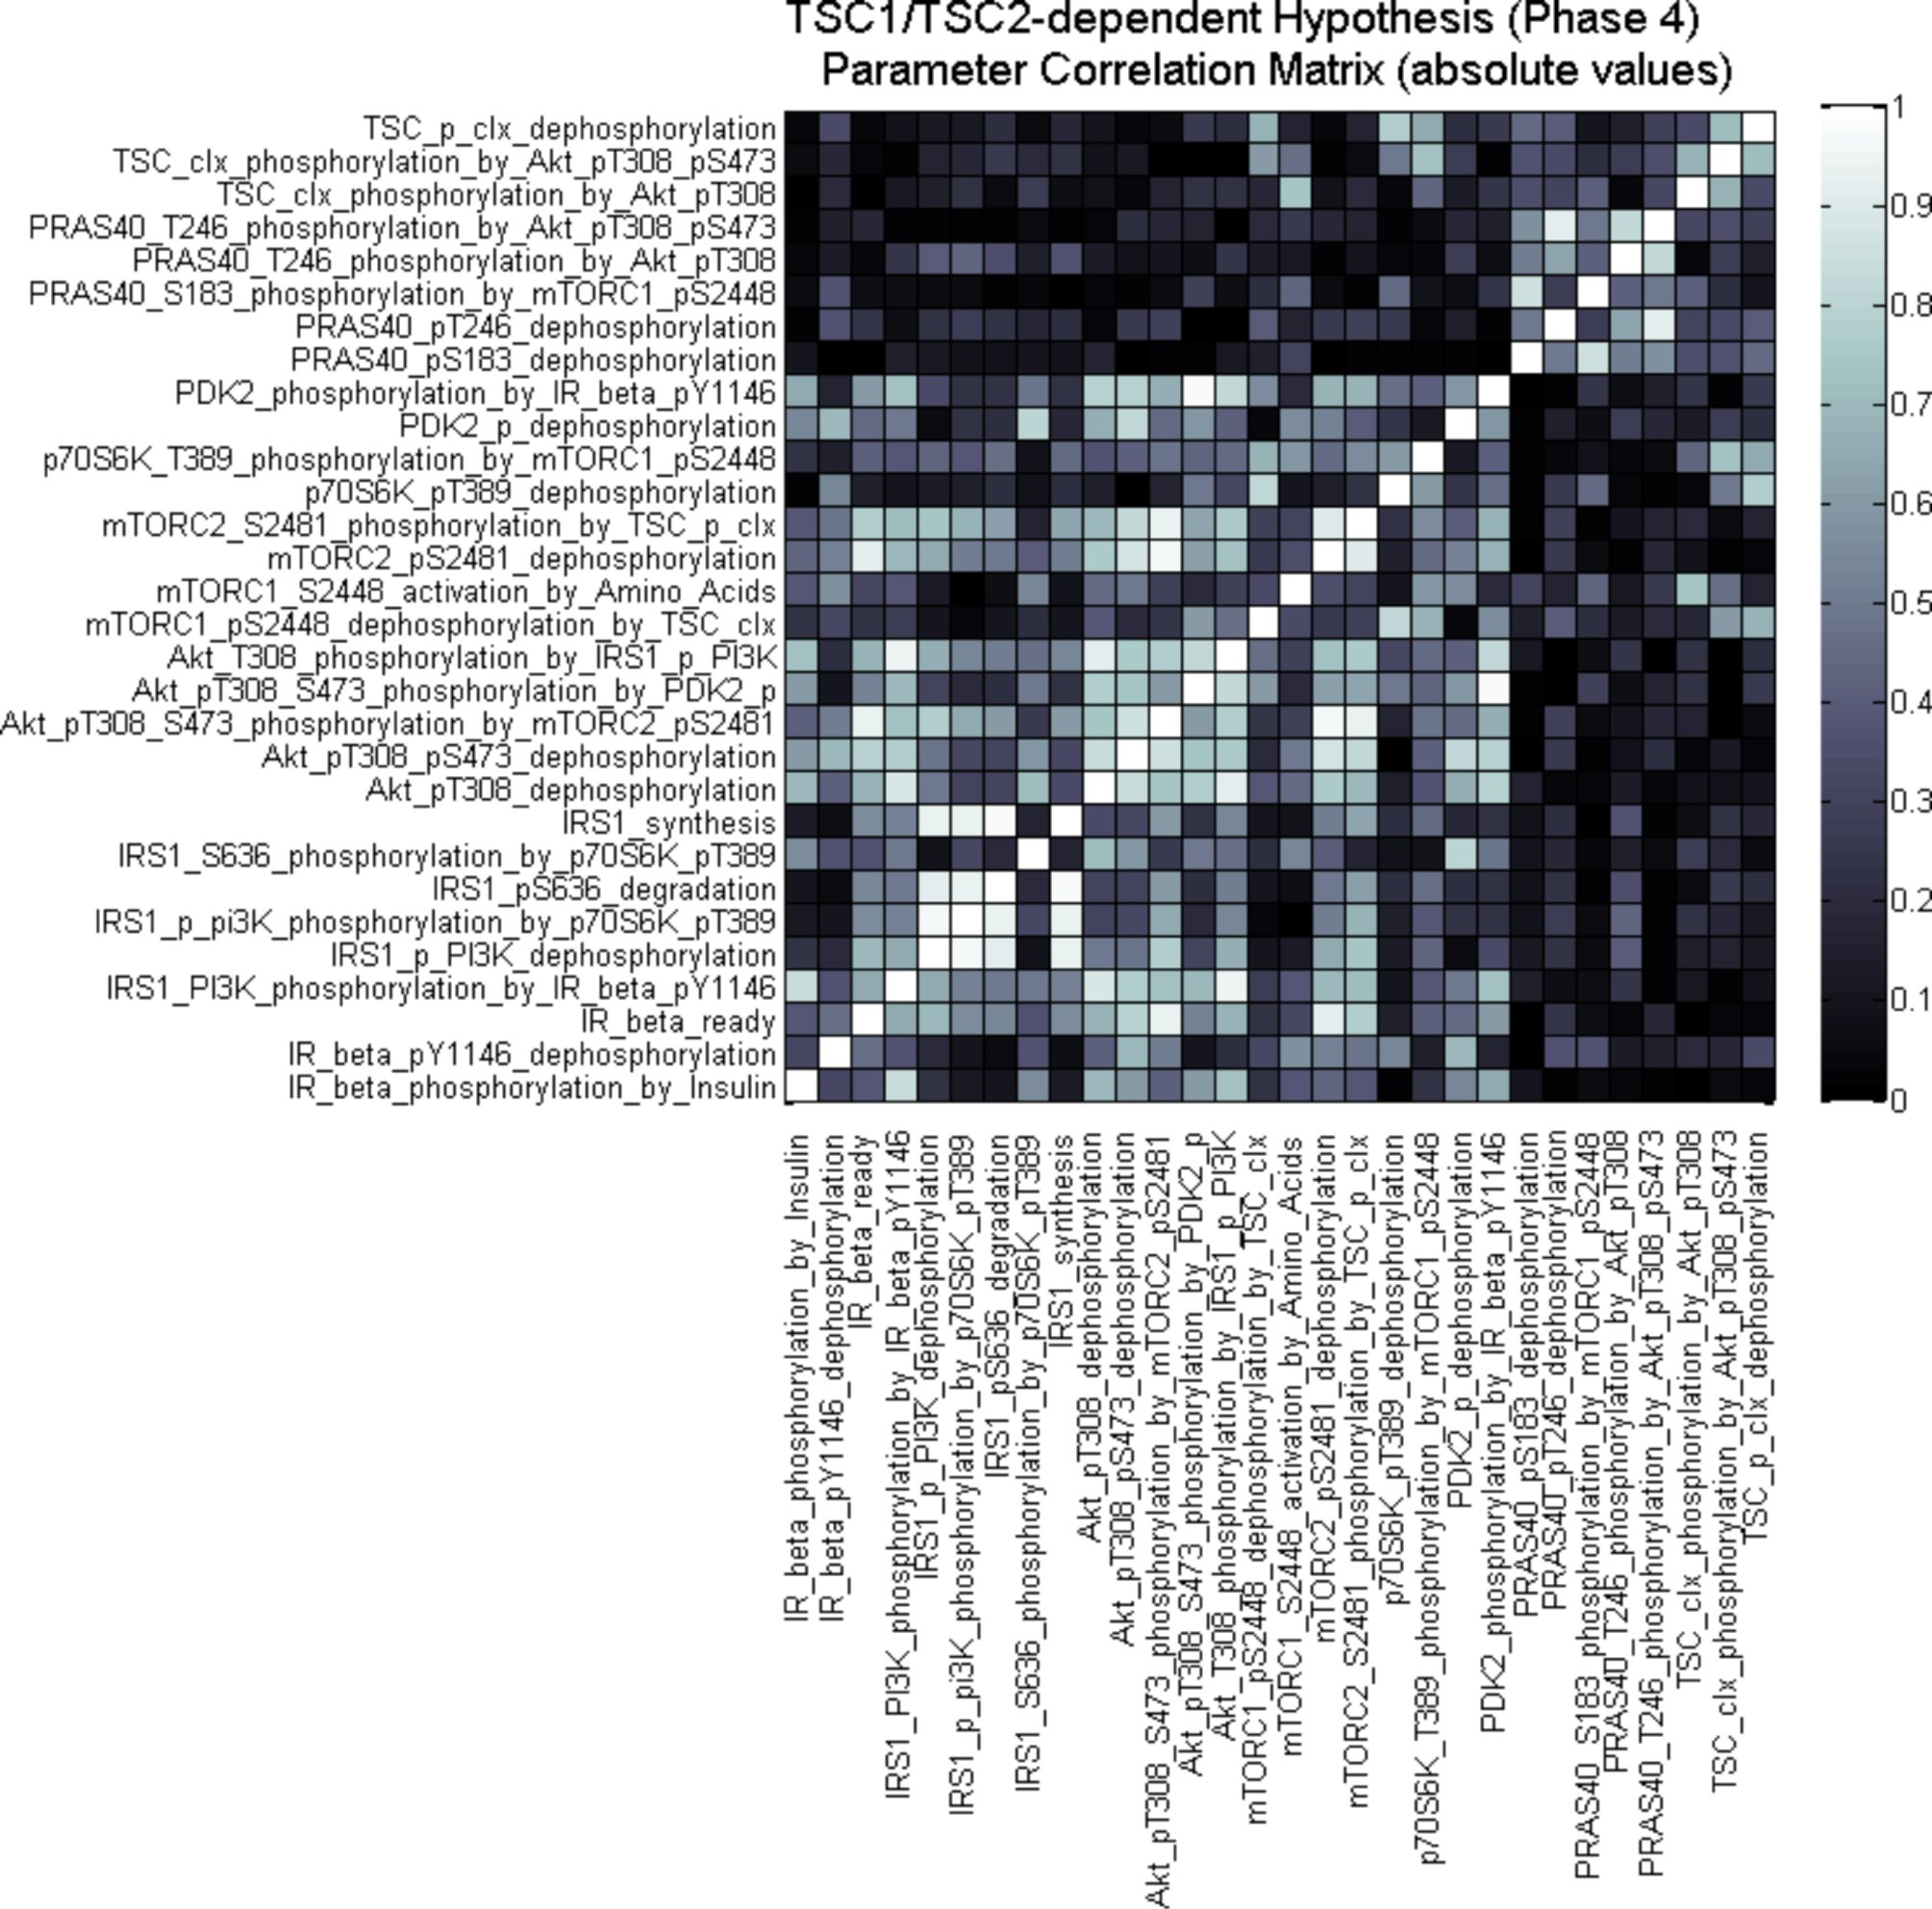
\includegraphics[scale=0.8]{2002469_supp_fig8.jpg}
		\caption[Identifiability analysis for Hypothesis 1: TSC1/TSC2-dependent mTORC2 regulation]{Identifiability analysis for Hypothesis 1: TSC1/TSC2-dependent mTORC2 regulation. Parameter correlation matrix for TSC1/TSC2-dependent hypothesis is shown. See Figure \ref{fig:2002469_supp_fig5} for details.}
		\label{fig:2002469_supp_fig8}
	\end{center}
\end{figure}
\clearpage

\begin{figure}[tb]
	\begin{center}
		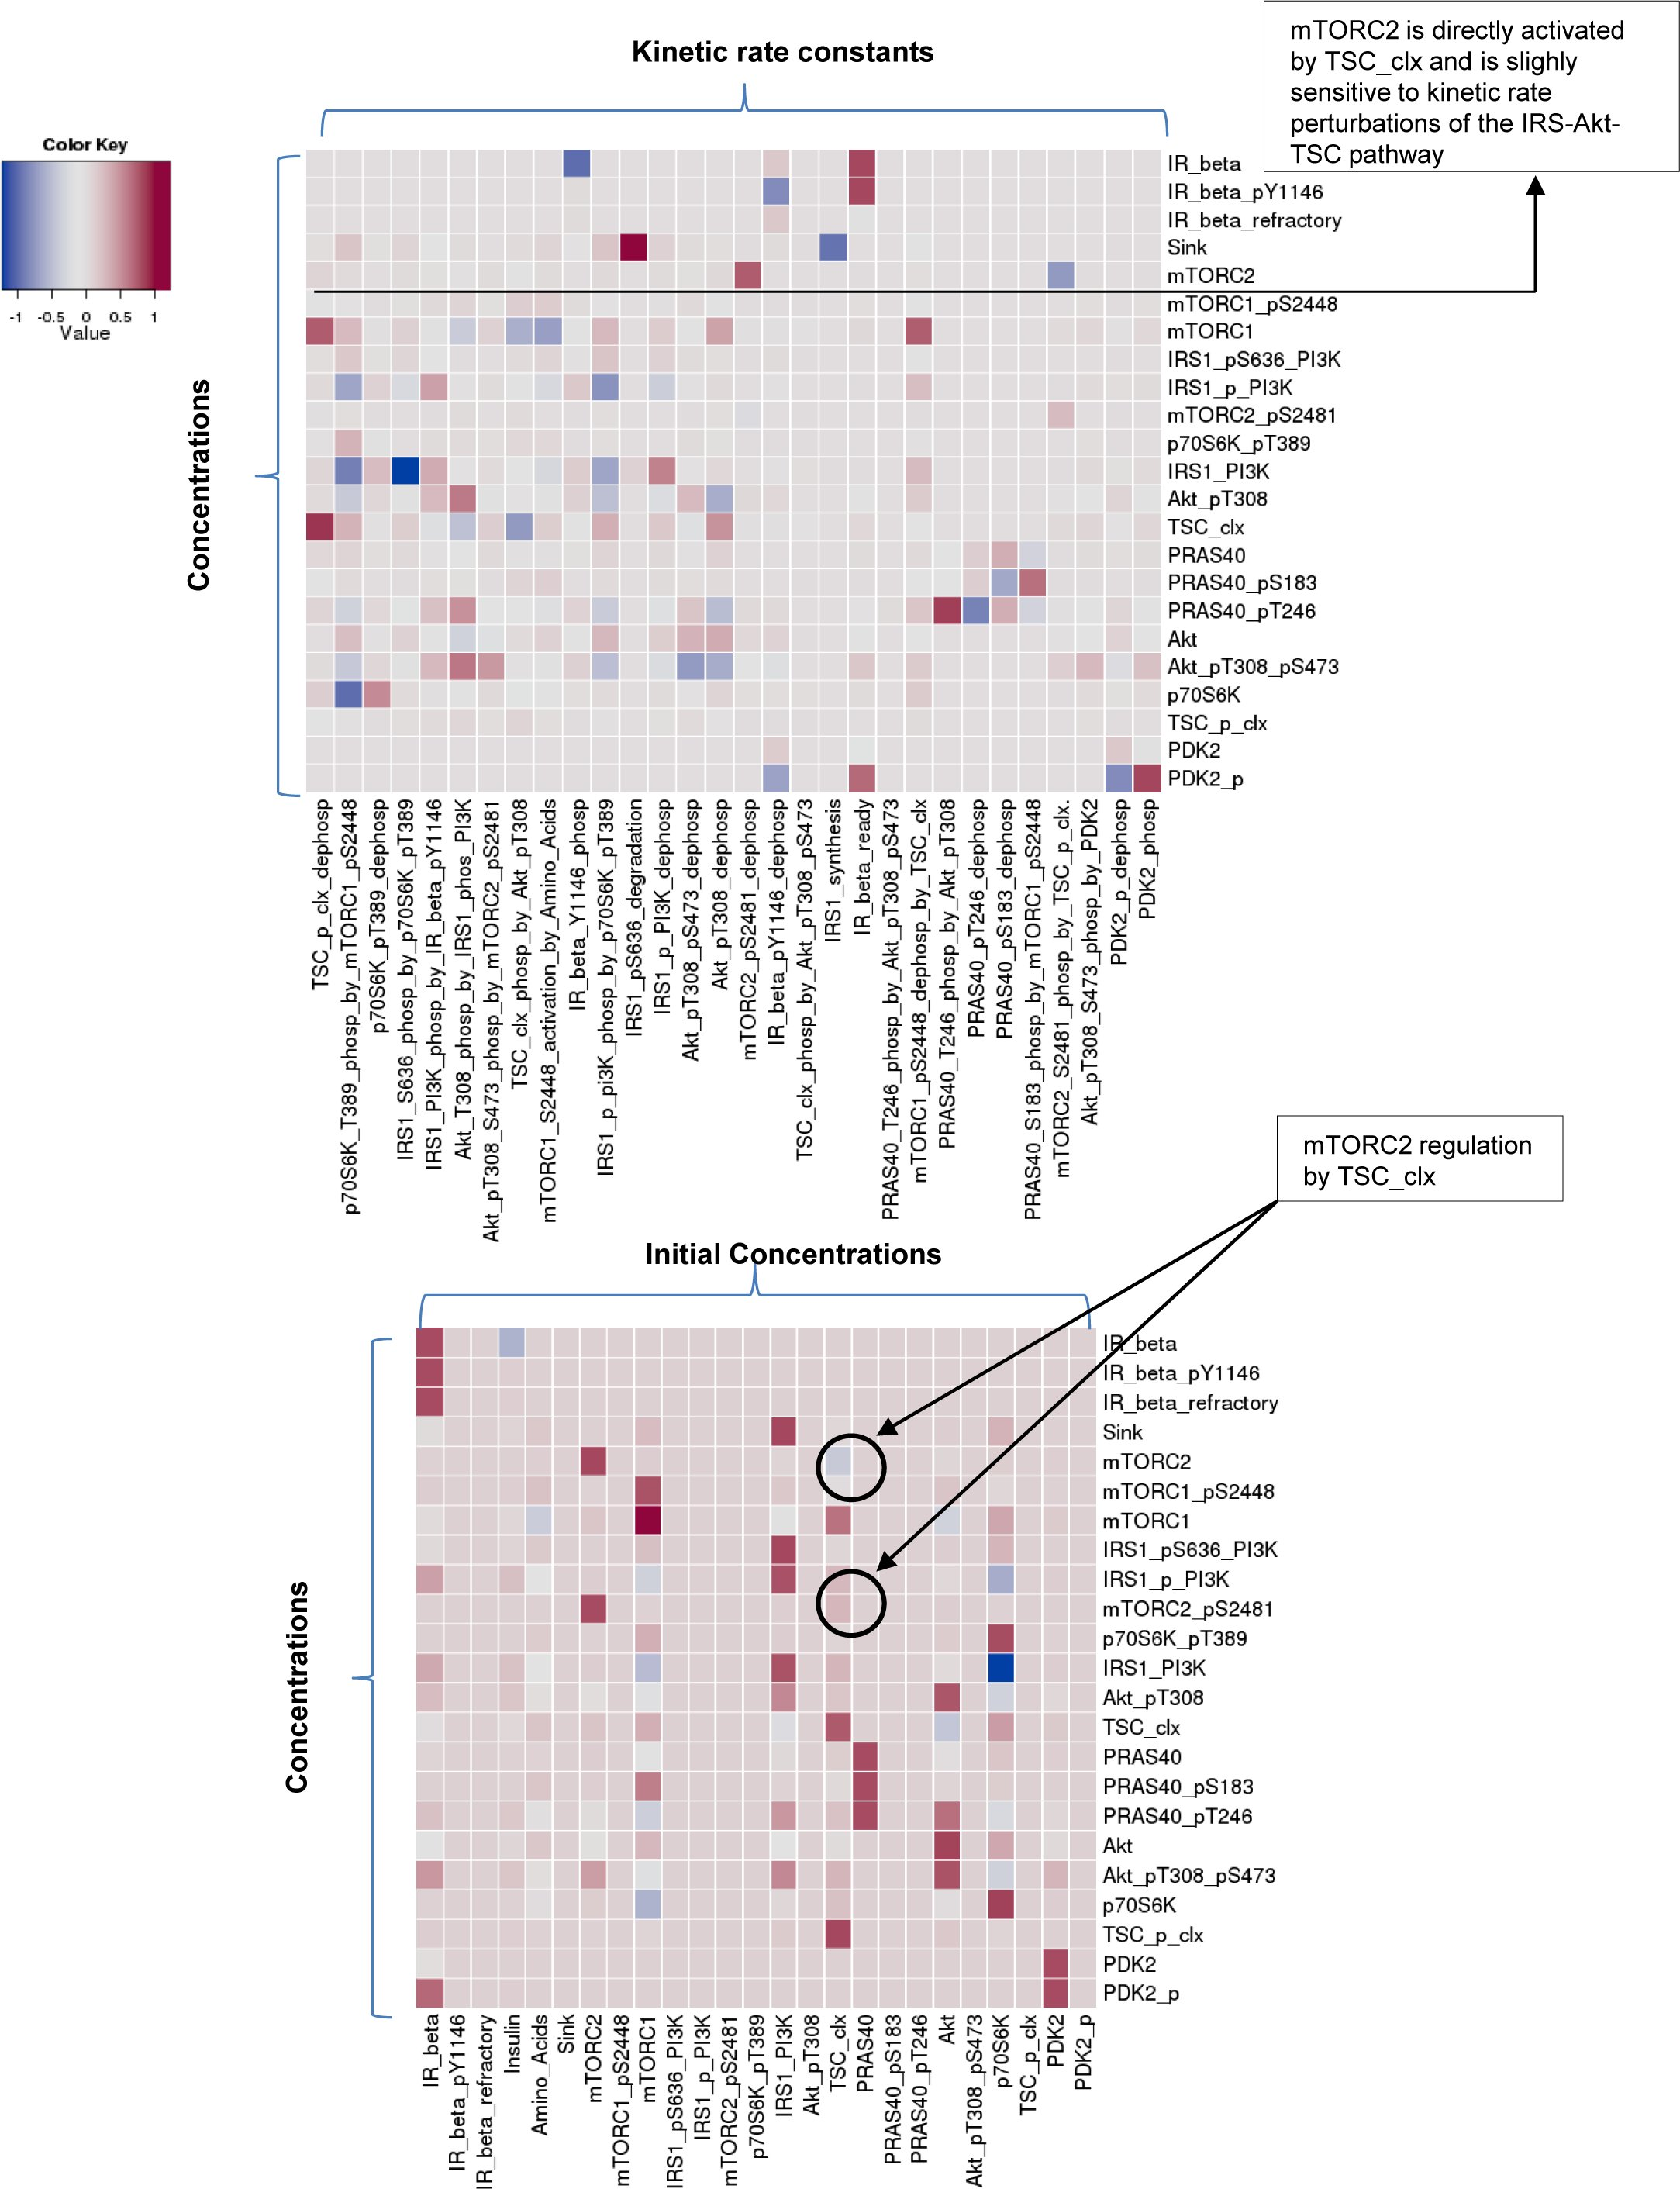
\includegraphics[width=5.10in]{2002469_supp_fig9.jpg}
		%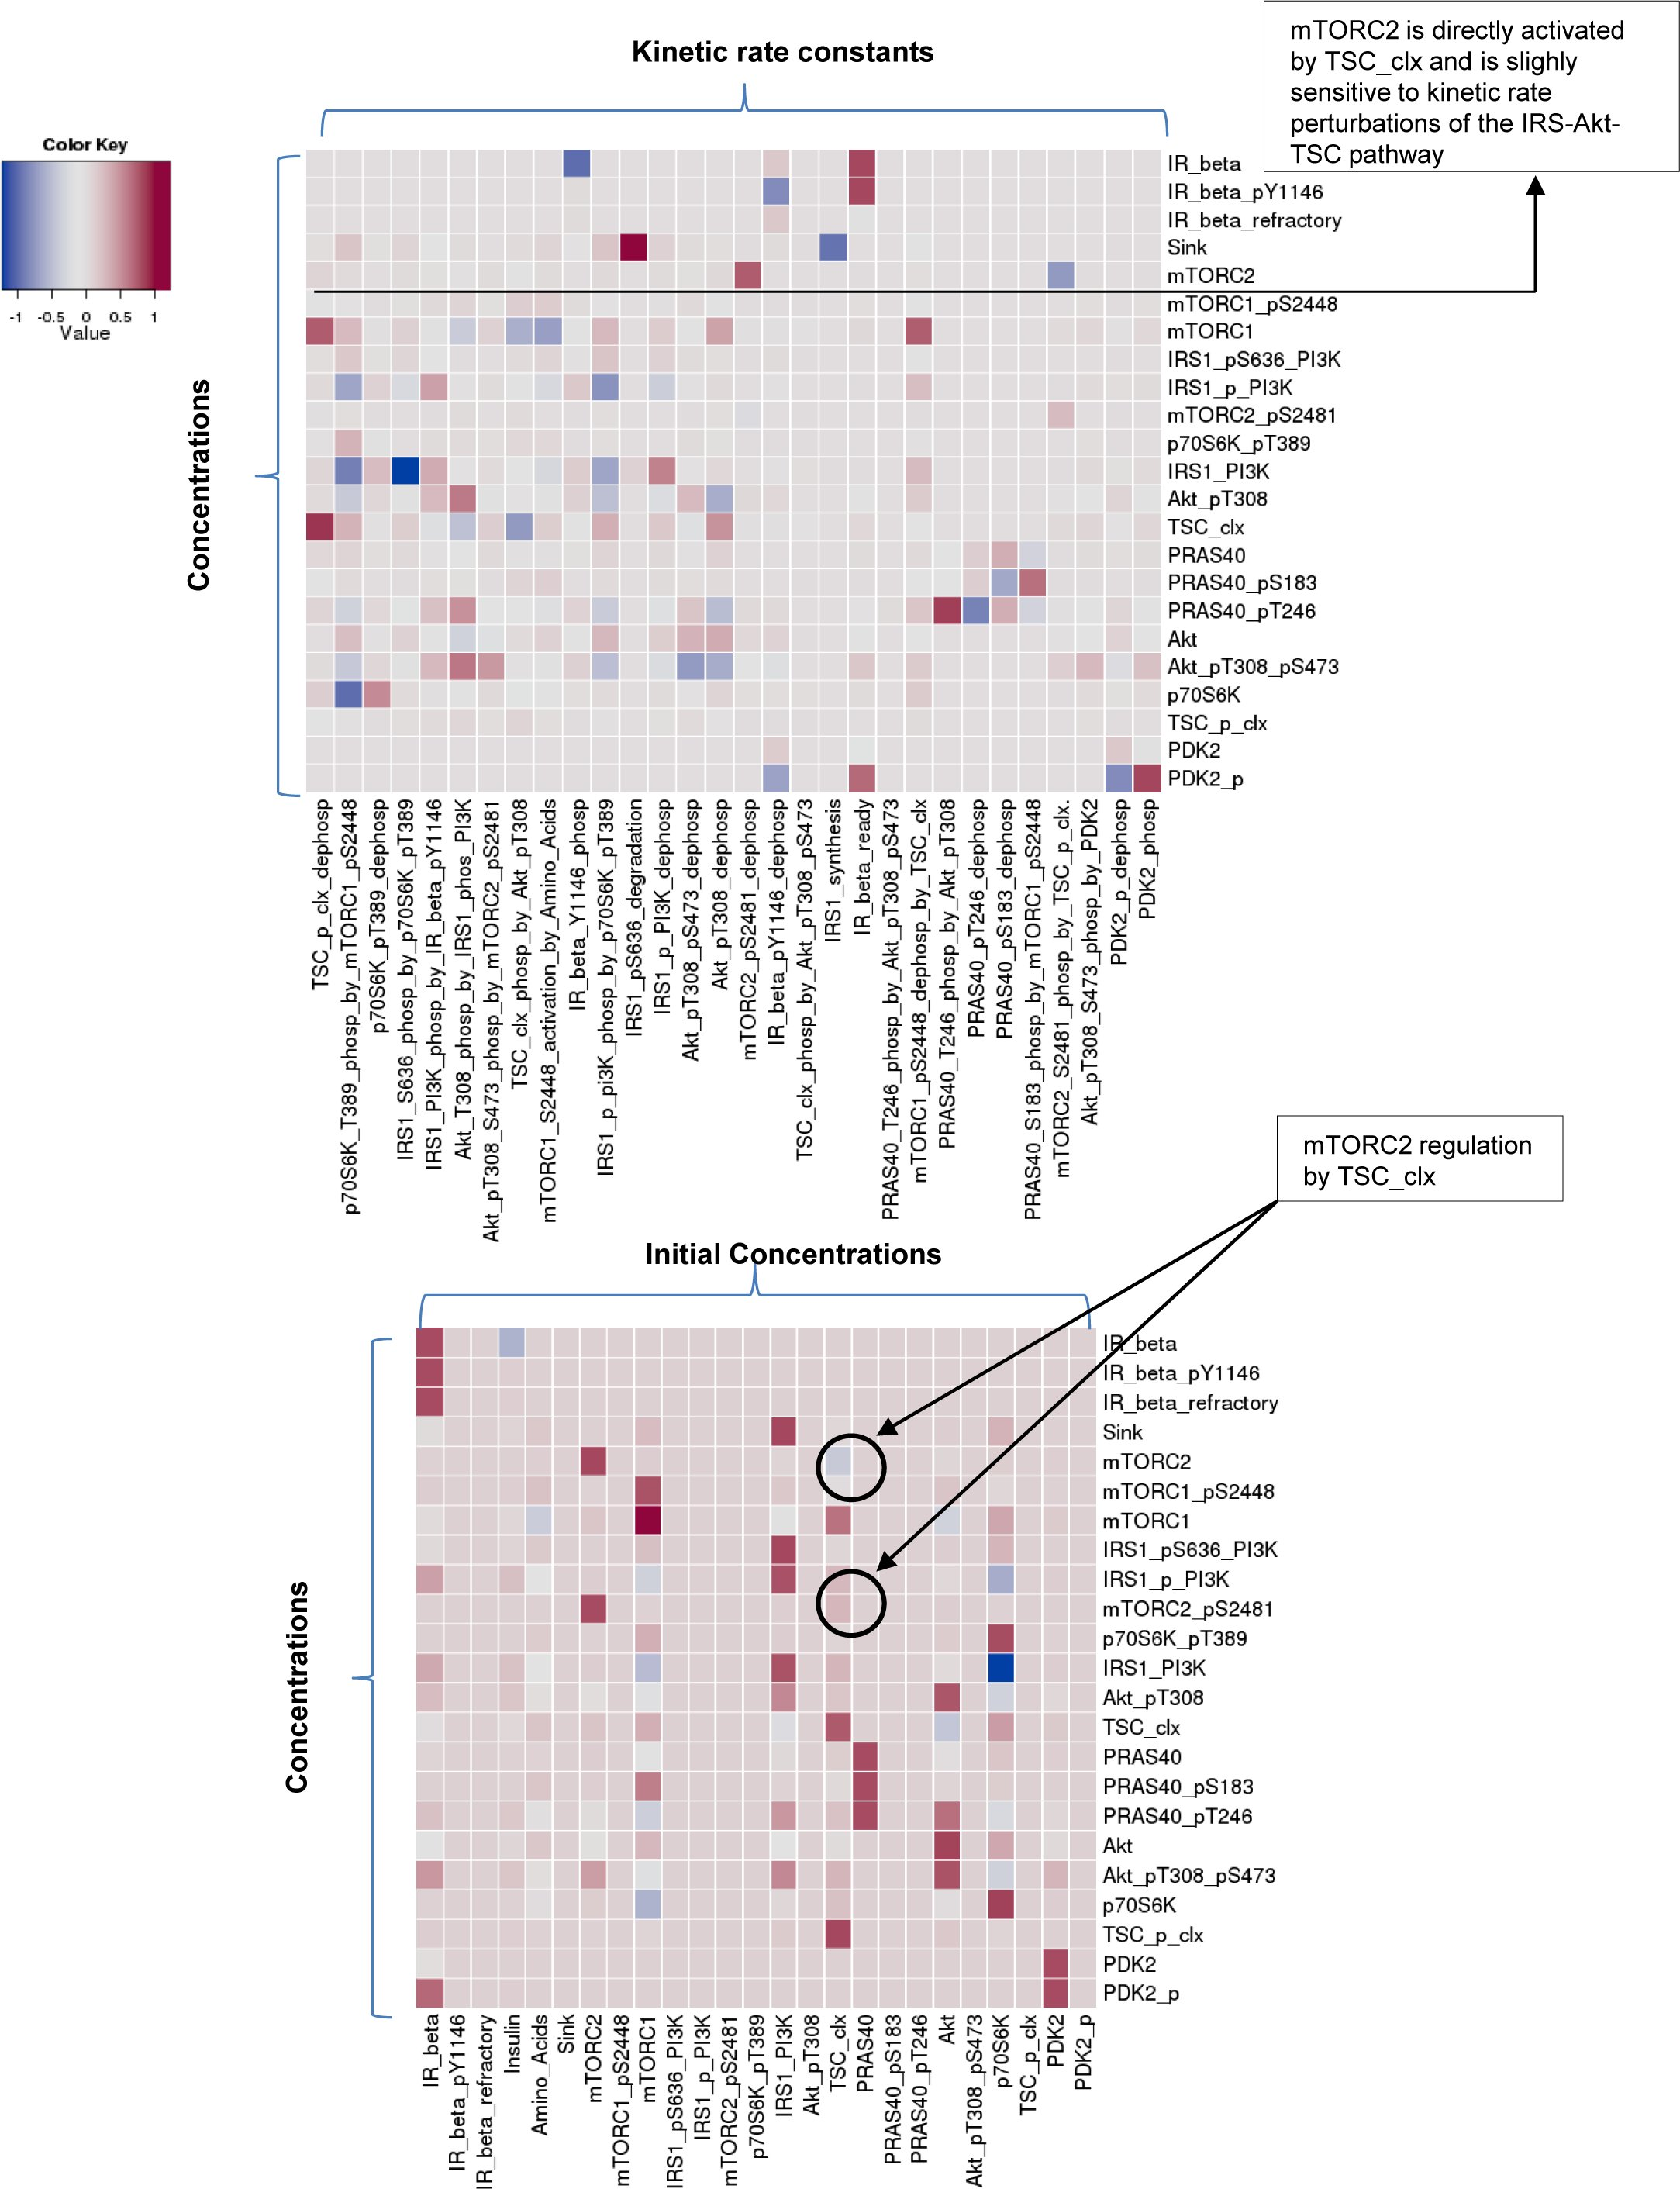
\includegraphics[scale=0.75]{2002469_supp_fig9.jpg}
		\caption[Sensitivity analysis for Hypothesis 1: TSC1/TSC2-dependent mTORC2 regulation]{Sensitivity analysis for Hypothesis 1: TSC1/TSC2-dependent mTORC2 regulation. The sensitivity analyses of the three hypotheses (see Figures \ref{fig:2002469_supp_fig11} and \ref{fig:2002469_supp_fig13}) showed a similar sensitivity analysis excluding the sensitivity for the parameters characterizing each specific hypothesis. This provided evidence that the proposed general model (common to the three hypotheses) behaved in a consistent manner following introduction of the three hypothetical models and, therefore, the three models were comparable. See Figure \ref{fig:2002469_supp_fig6} for details of the top and bottom plots.}
		\label{fig:2002469_supp_fig9}
	\end{center}
\end{figure}
\clearpage

\begin{figure}[tb]
	\begin{center}
		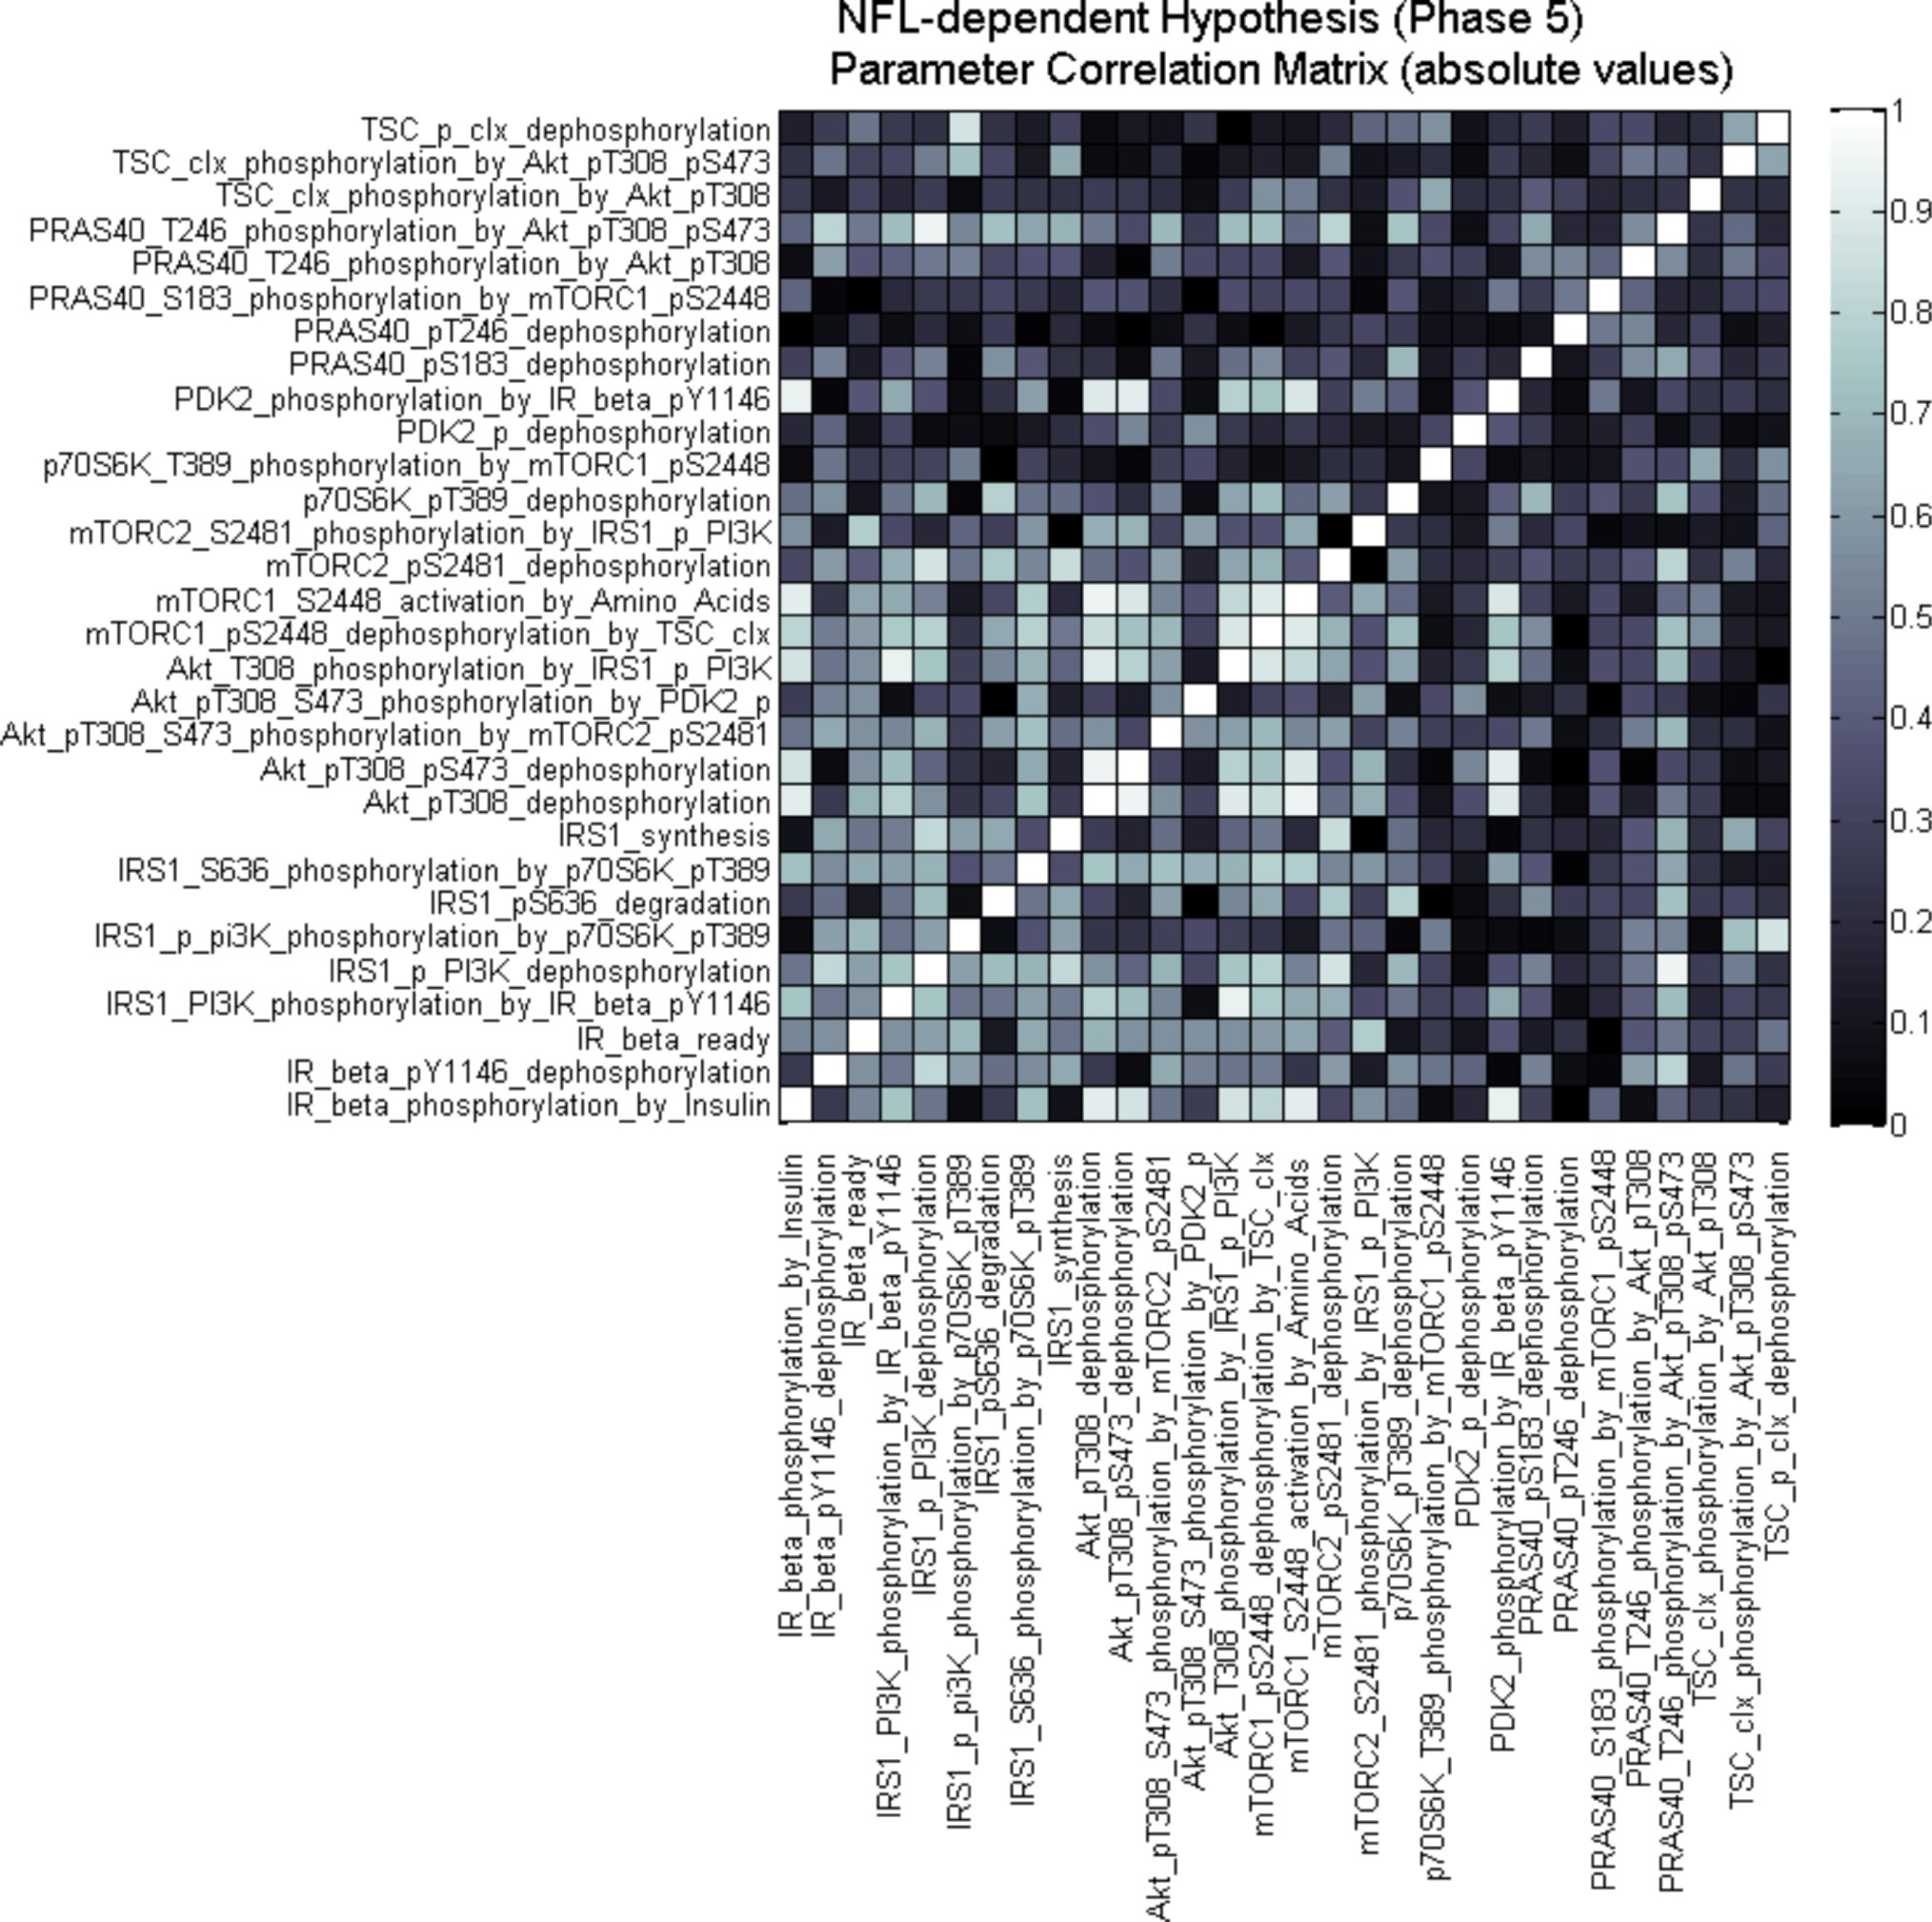
\includegraphics[scale=0.8]{2002469_supp_fig10.jpg}
		\caption[Identifiability analysis for Hypothesis 2: NFL-dependent mTORC2 regulation]{Identifiability analysis for Hypothesis 2: NFL-dependent mTORC2 regulation. Parameter correlation matrix for NFL-dependent hypothesis is shown. See Figure \ref{fig:2002469_supp_fig5} for details.}
		\label{fig:2002469_supp_fig10}
	\end{center}
\end{figure}
\clearpage

\begin{figure}[tb]
	\begin{center}
		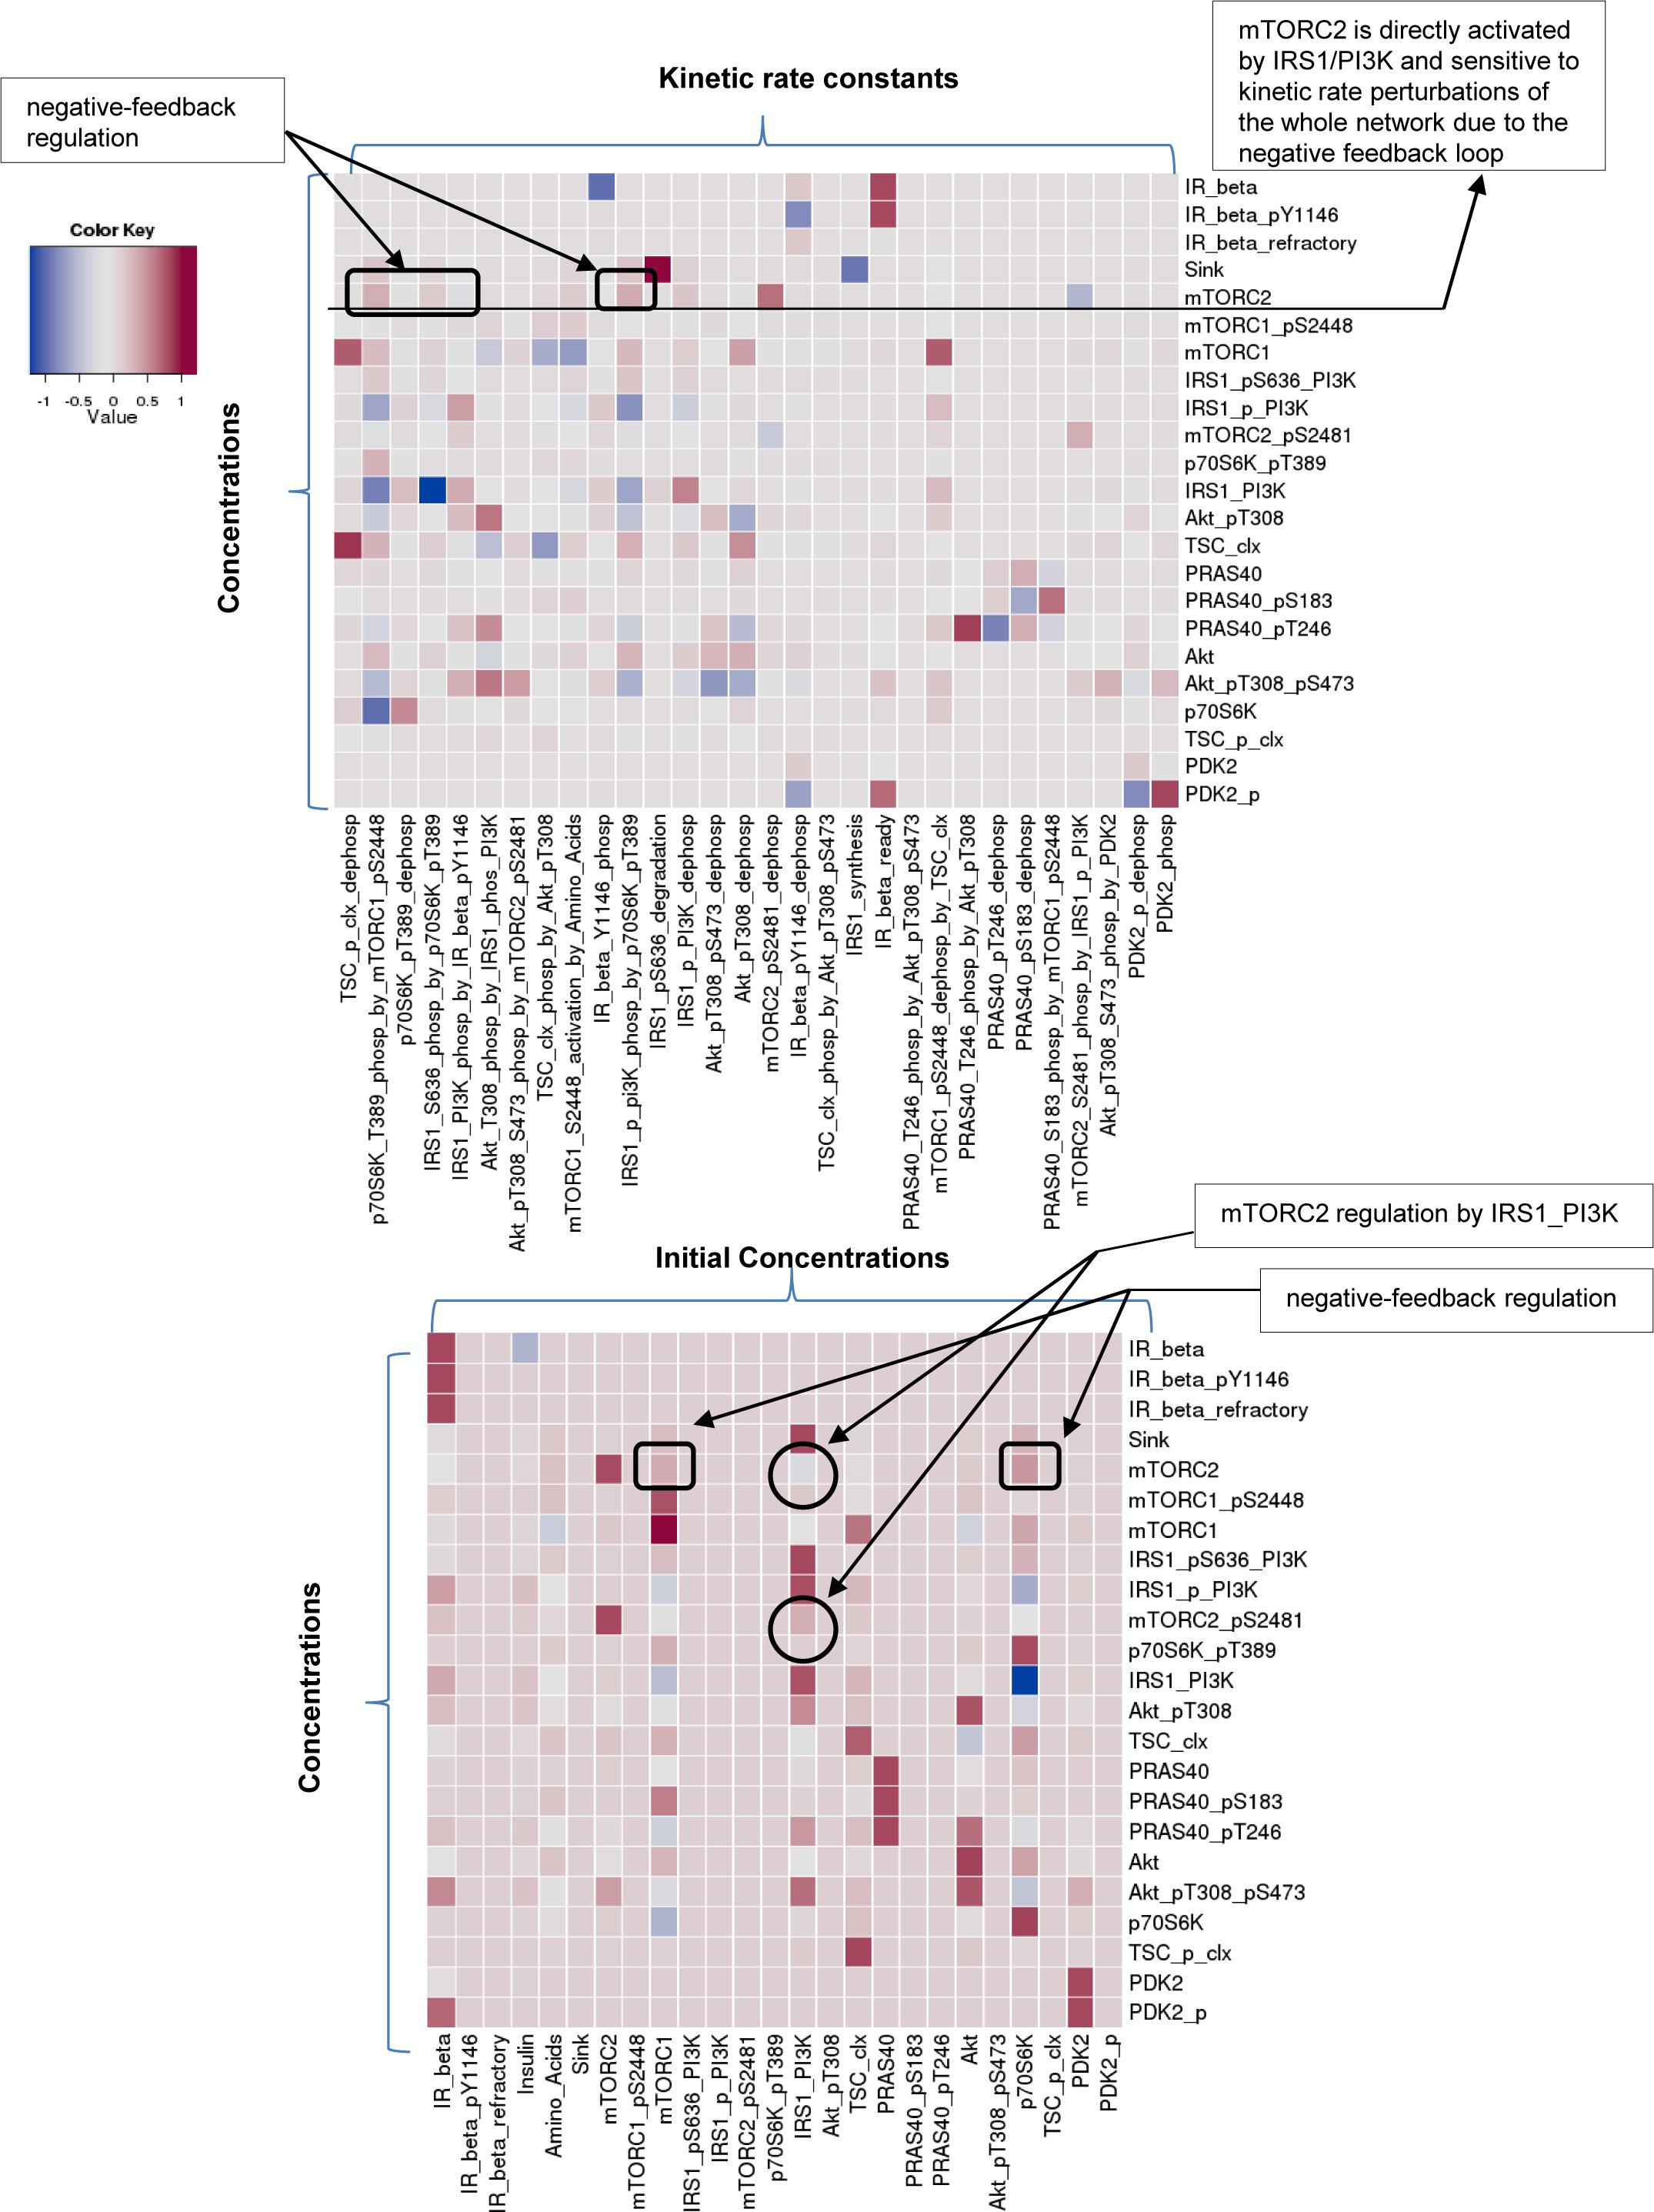
\includegraphics[scale=0.75]{2002469_supp_fig11.jpg}
		\caption[Sensitivity analysis for Hypothesis 2: NFL-dependent mTORC2 regulation]{Sensitivity analysis for Hypothesis 2: NFL-dependent mTORC2 regulation. Sensitivity analysis for the initial concentrations and the kinetic rates parameters for the NFL-dependent hypothesis is shown.  See Figure \ref{fig:2002469_supp_fig6} for details of the top and bottom plots.}
		\label{fig:2002469_supp_fig11}
	\end{center}
\end{figure}
\clearpage

\begin{figure}[tb]
	\begin{center}
		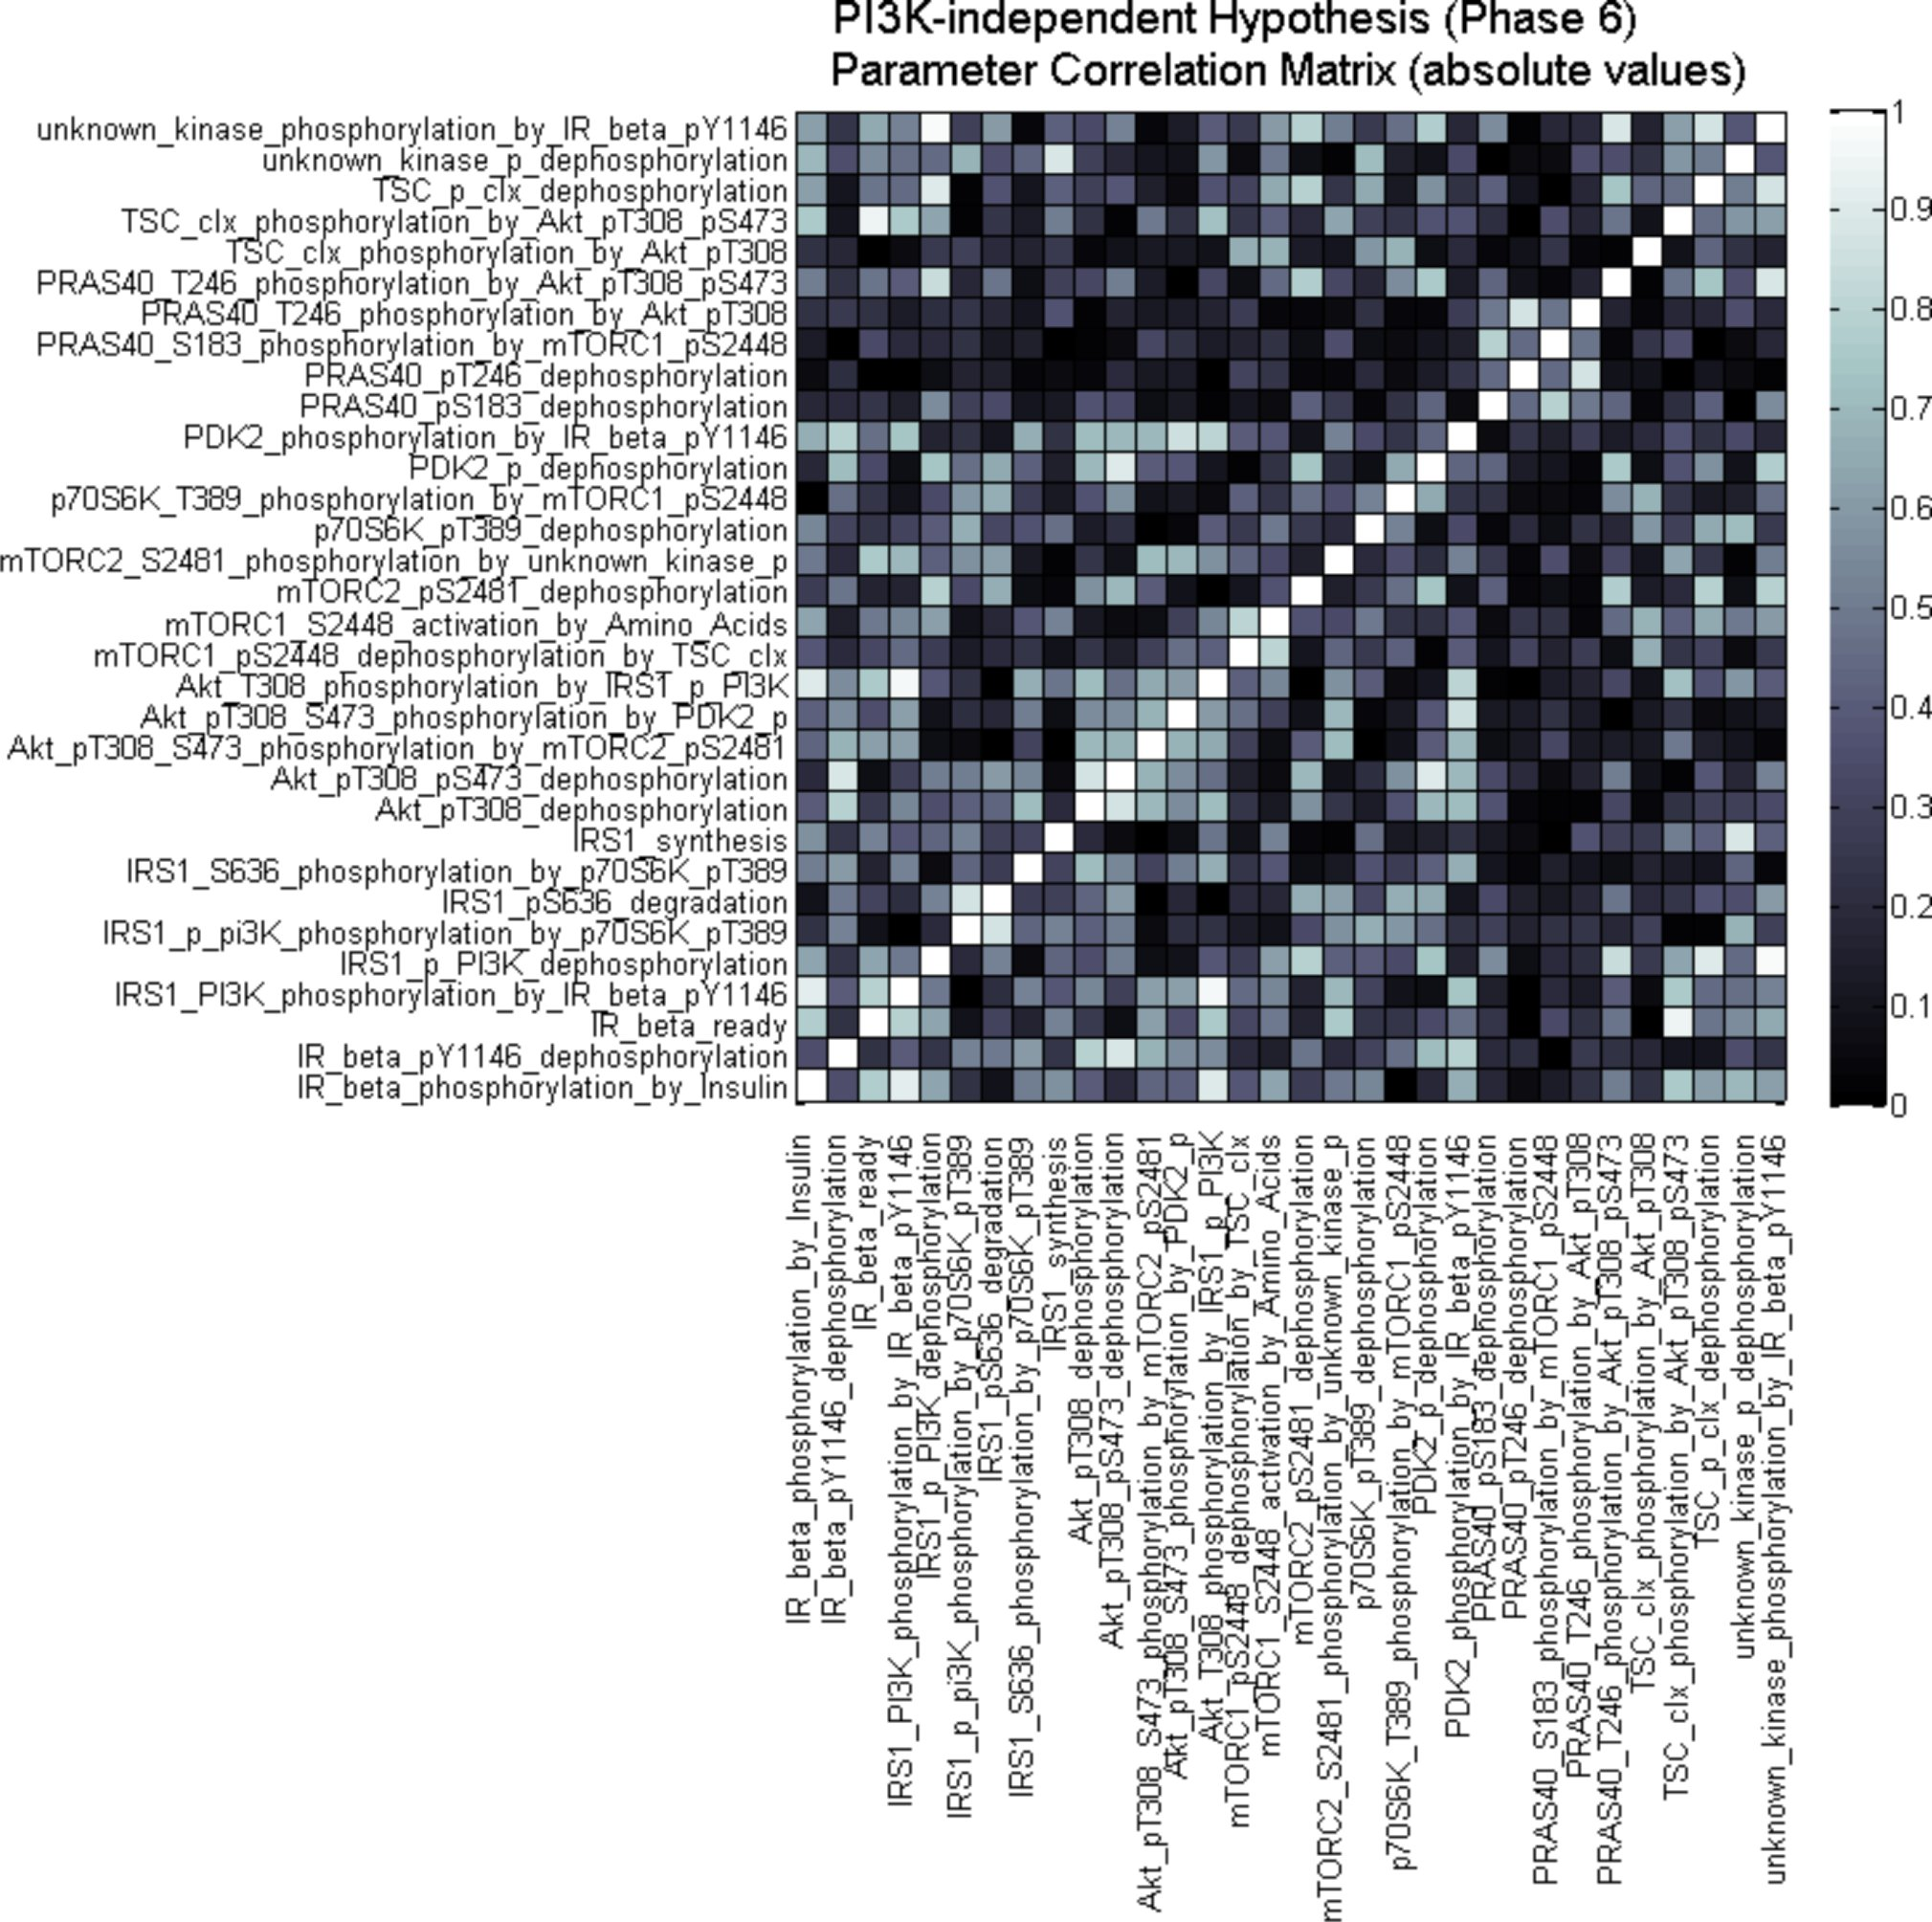
\includegraphics[scale=0.8]{2002469_supp_fig12.jpg}
		\caption[Identifiability analysis for Hypothesis 3: PI3K-independent mTORC2 regulation]{Identifiability analysis for Hypothesis 3: PI3K-independent mTORC2 regulation. Parameter correlation matrix for PI3K-independent hypothesis is shown. See Figure \ref{fig:2002469_supp_fig5} for details.}
		\label{fig:2002469_supp_fig12}
	\end{center}
\end{figure}
\clearpage

\begin{figure}[tb]
	\begin{center}
		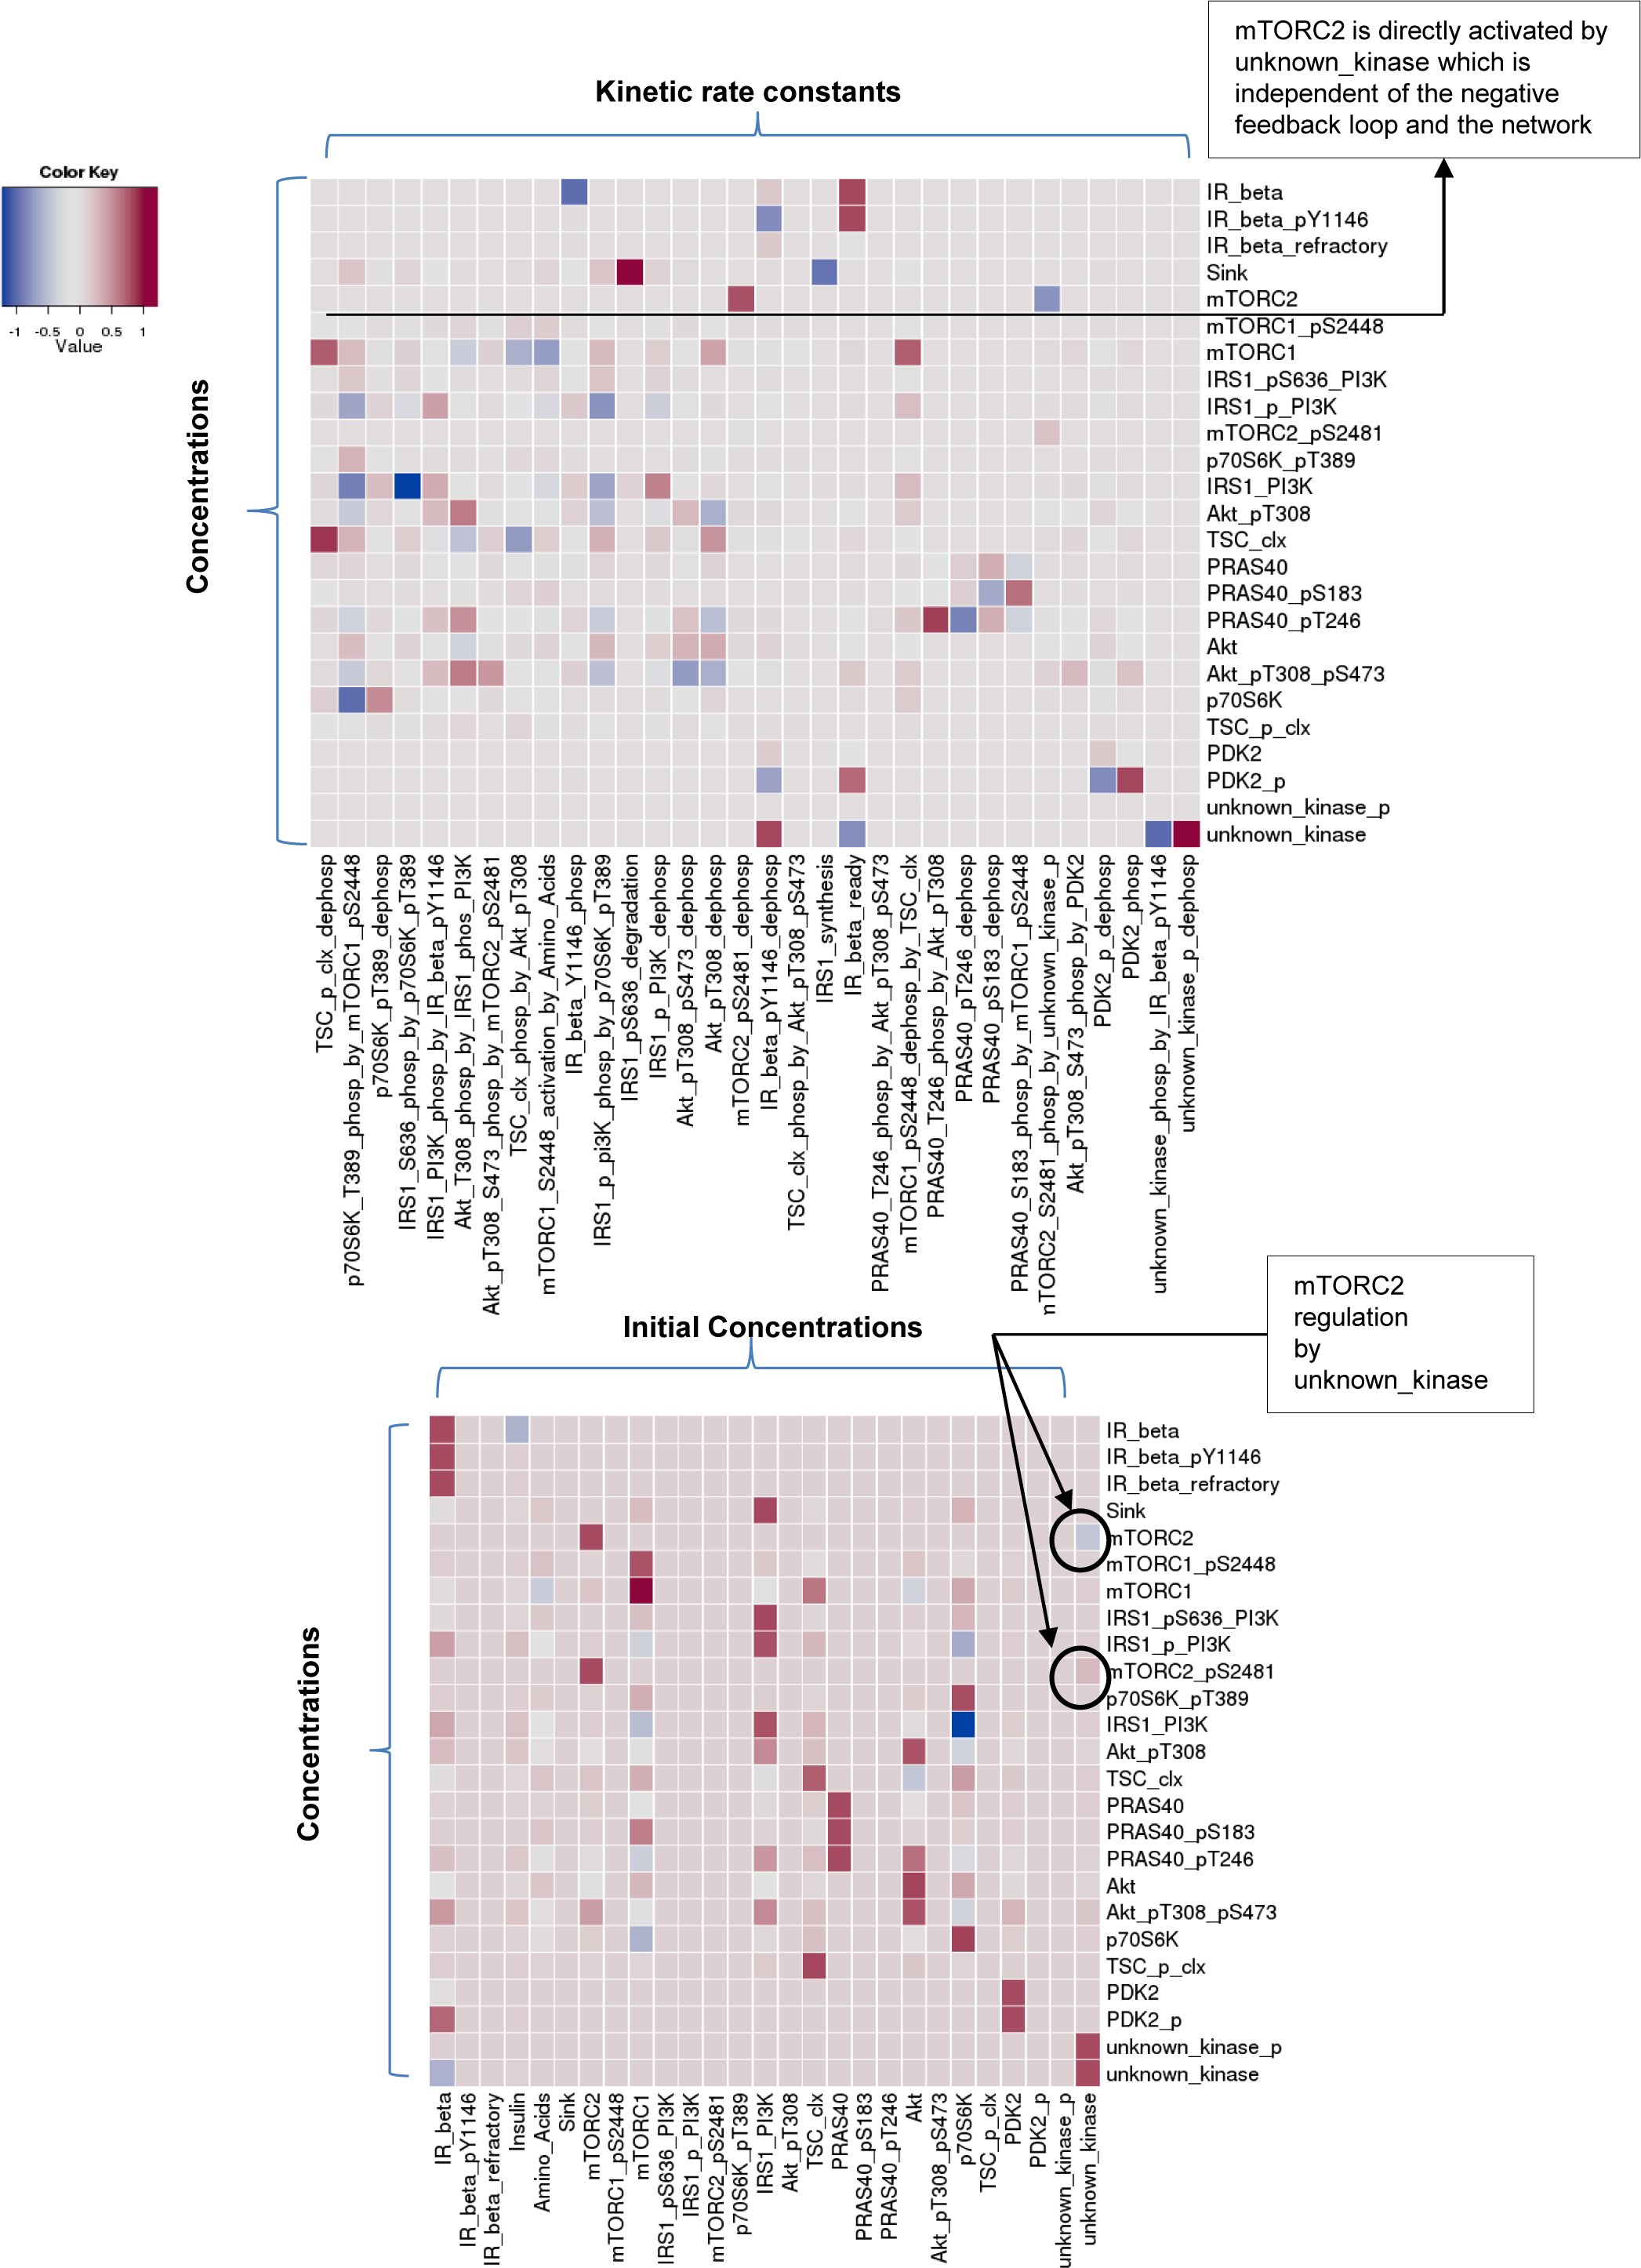
\includegraphics[scale=0.75]{2002469_supp_fig13.jpg}
		\caption[Sensitivity analysis for Hypothesis 3: PI3K-independent mTORC2 regulation]{Sensitivity analysis for Hypothesis 3: PI3K-independent mTORC2 regulation. Sensitivity analysis for the initial concentrations and the kinetic rates parameters for the PI3K-independent hypothesis is shown. See Figure \ref{fig:2002469_supp_fig6} for details of the top and bottom plots.}
		\label{fig:2002469_supp_fig13}
	\end{center}
\end{figure}
\clearpage

\begin{figure}[tb]
	\begin{center}
		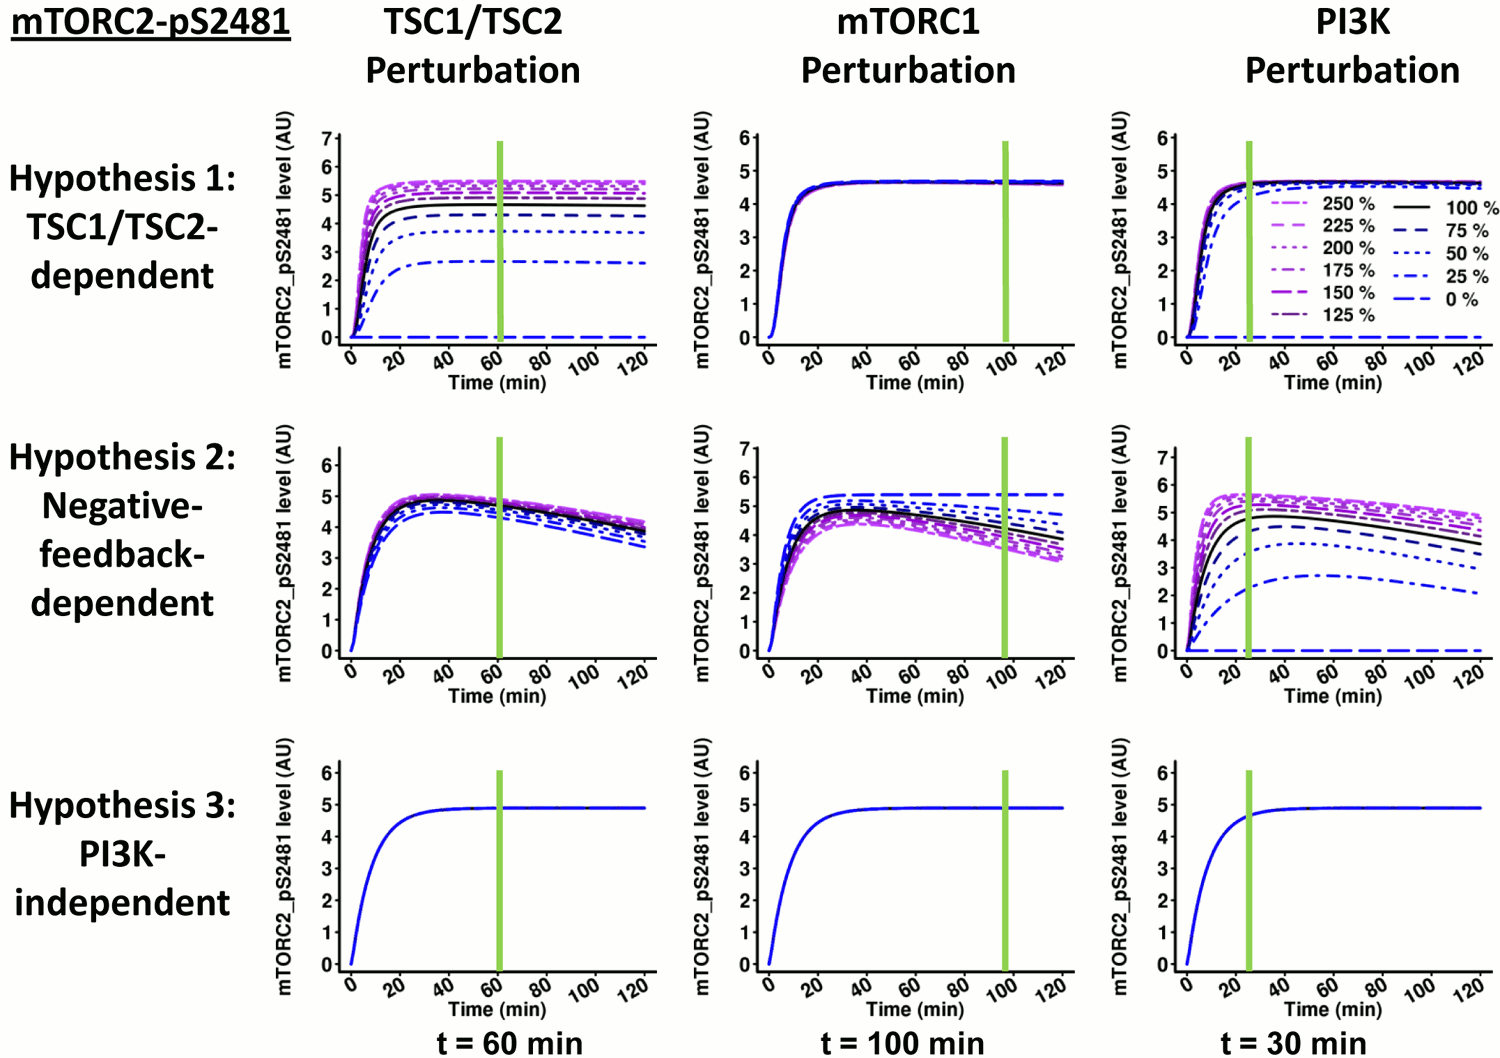
\includegraphics[scale=1.1]{2002469_fig5A.png}
		\caption[Simulations of network perturbations at several levels and differential dynamical network responses for the three different hypotheses (mTOR-pS2481 readout)]{Simulations of network perturbations at several levels and differential dynamical network responses for the three different hypotheses (mTOR-pS2481 readout). Simulated mTOR-pS2481 response upon amino acids/insulin induction in systems with the indicated perturbations: TSC1/TSC2 (experimental equivalent: gradual TSC2 knockdown), mTORC1 (experimental equivalent: gradual Raptor knockdown), and PI3K (experimental equivalent: gradual PI3K inhibition with Wortmannin) for Hypothesis 1, 2, and 3. The time points that were experimentally tested are indicated with green lines.}
		\label{fig:2002469_fig5A}
	\end{center}
\end{figure}

\clearpage
\begin{figure}[tb]
	\begin{center}
		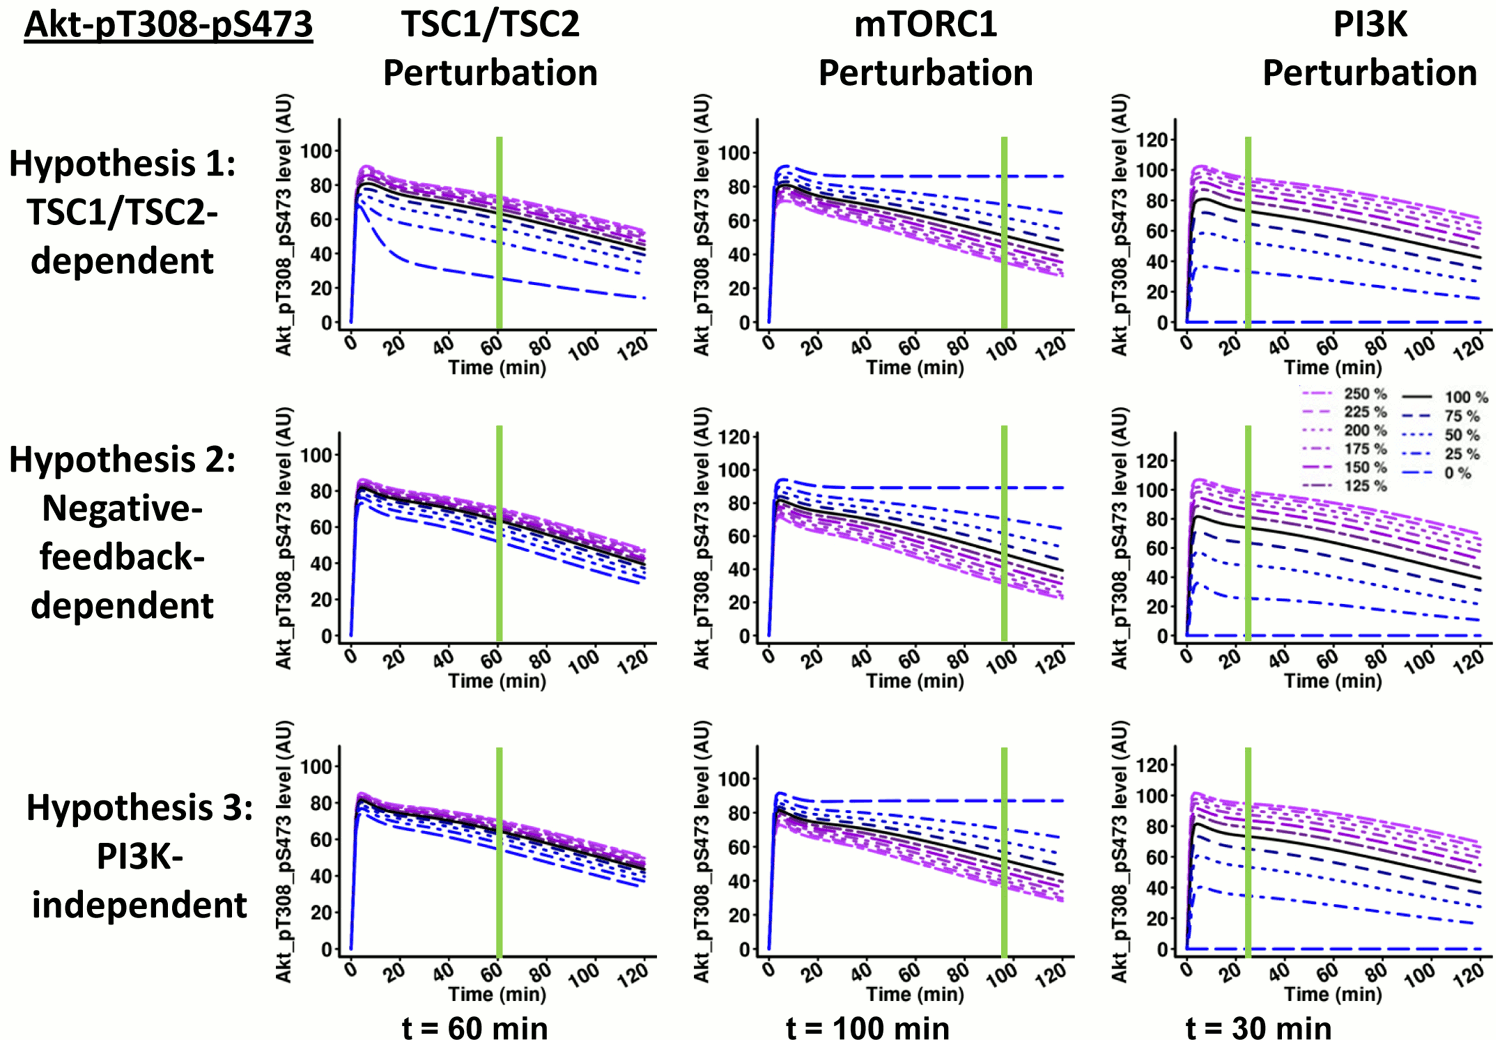
\includegraphics[scale=1.1]{2002469_fig5B.png}
		\caption[Simulations of network perturbations at several levels and differential dynamical network responses for the three different hypotheses (Akt-pS473 readout)]{Simulations of network perturbations at several levels and differential dynamical network responses for the three different hypotheses (Akt-pS473 readout). Simulated Akt-pT308-pS473 response for each of the three hypotheses upon amino acids/insulin induction in systems with perturbations of TSC1/TSC2, mTORC1, and PI3K. The time points that were experimentally tested are indicated with green lines.}
		\label{fig:2002469_fig5B}
	\end{center}
\end{figure}
\clearpage

\begin{figure}[tb]
	\begin{center}
		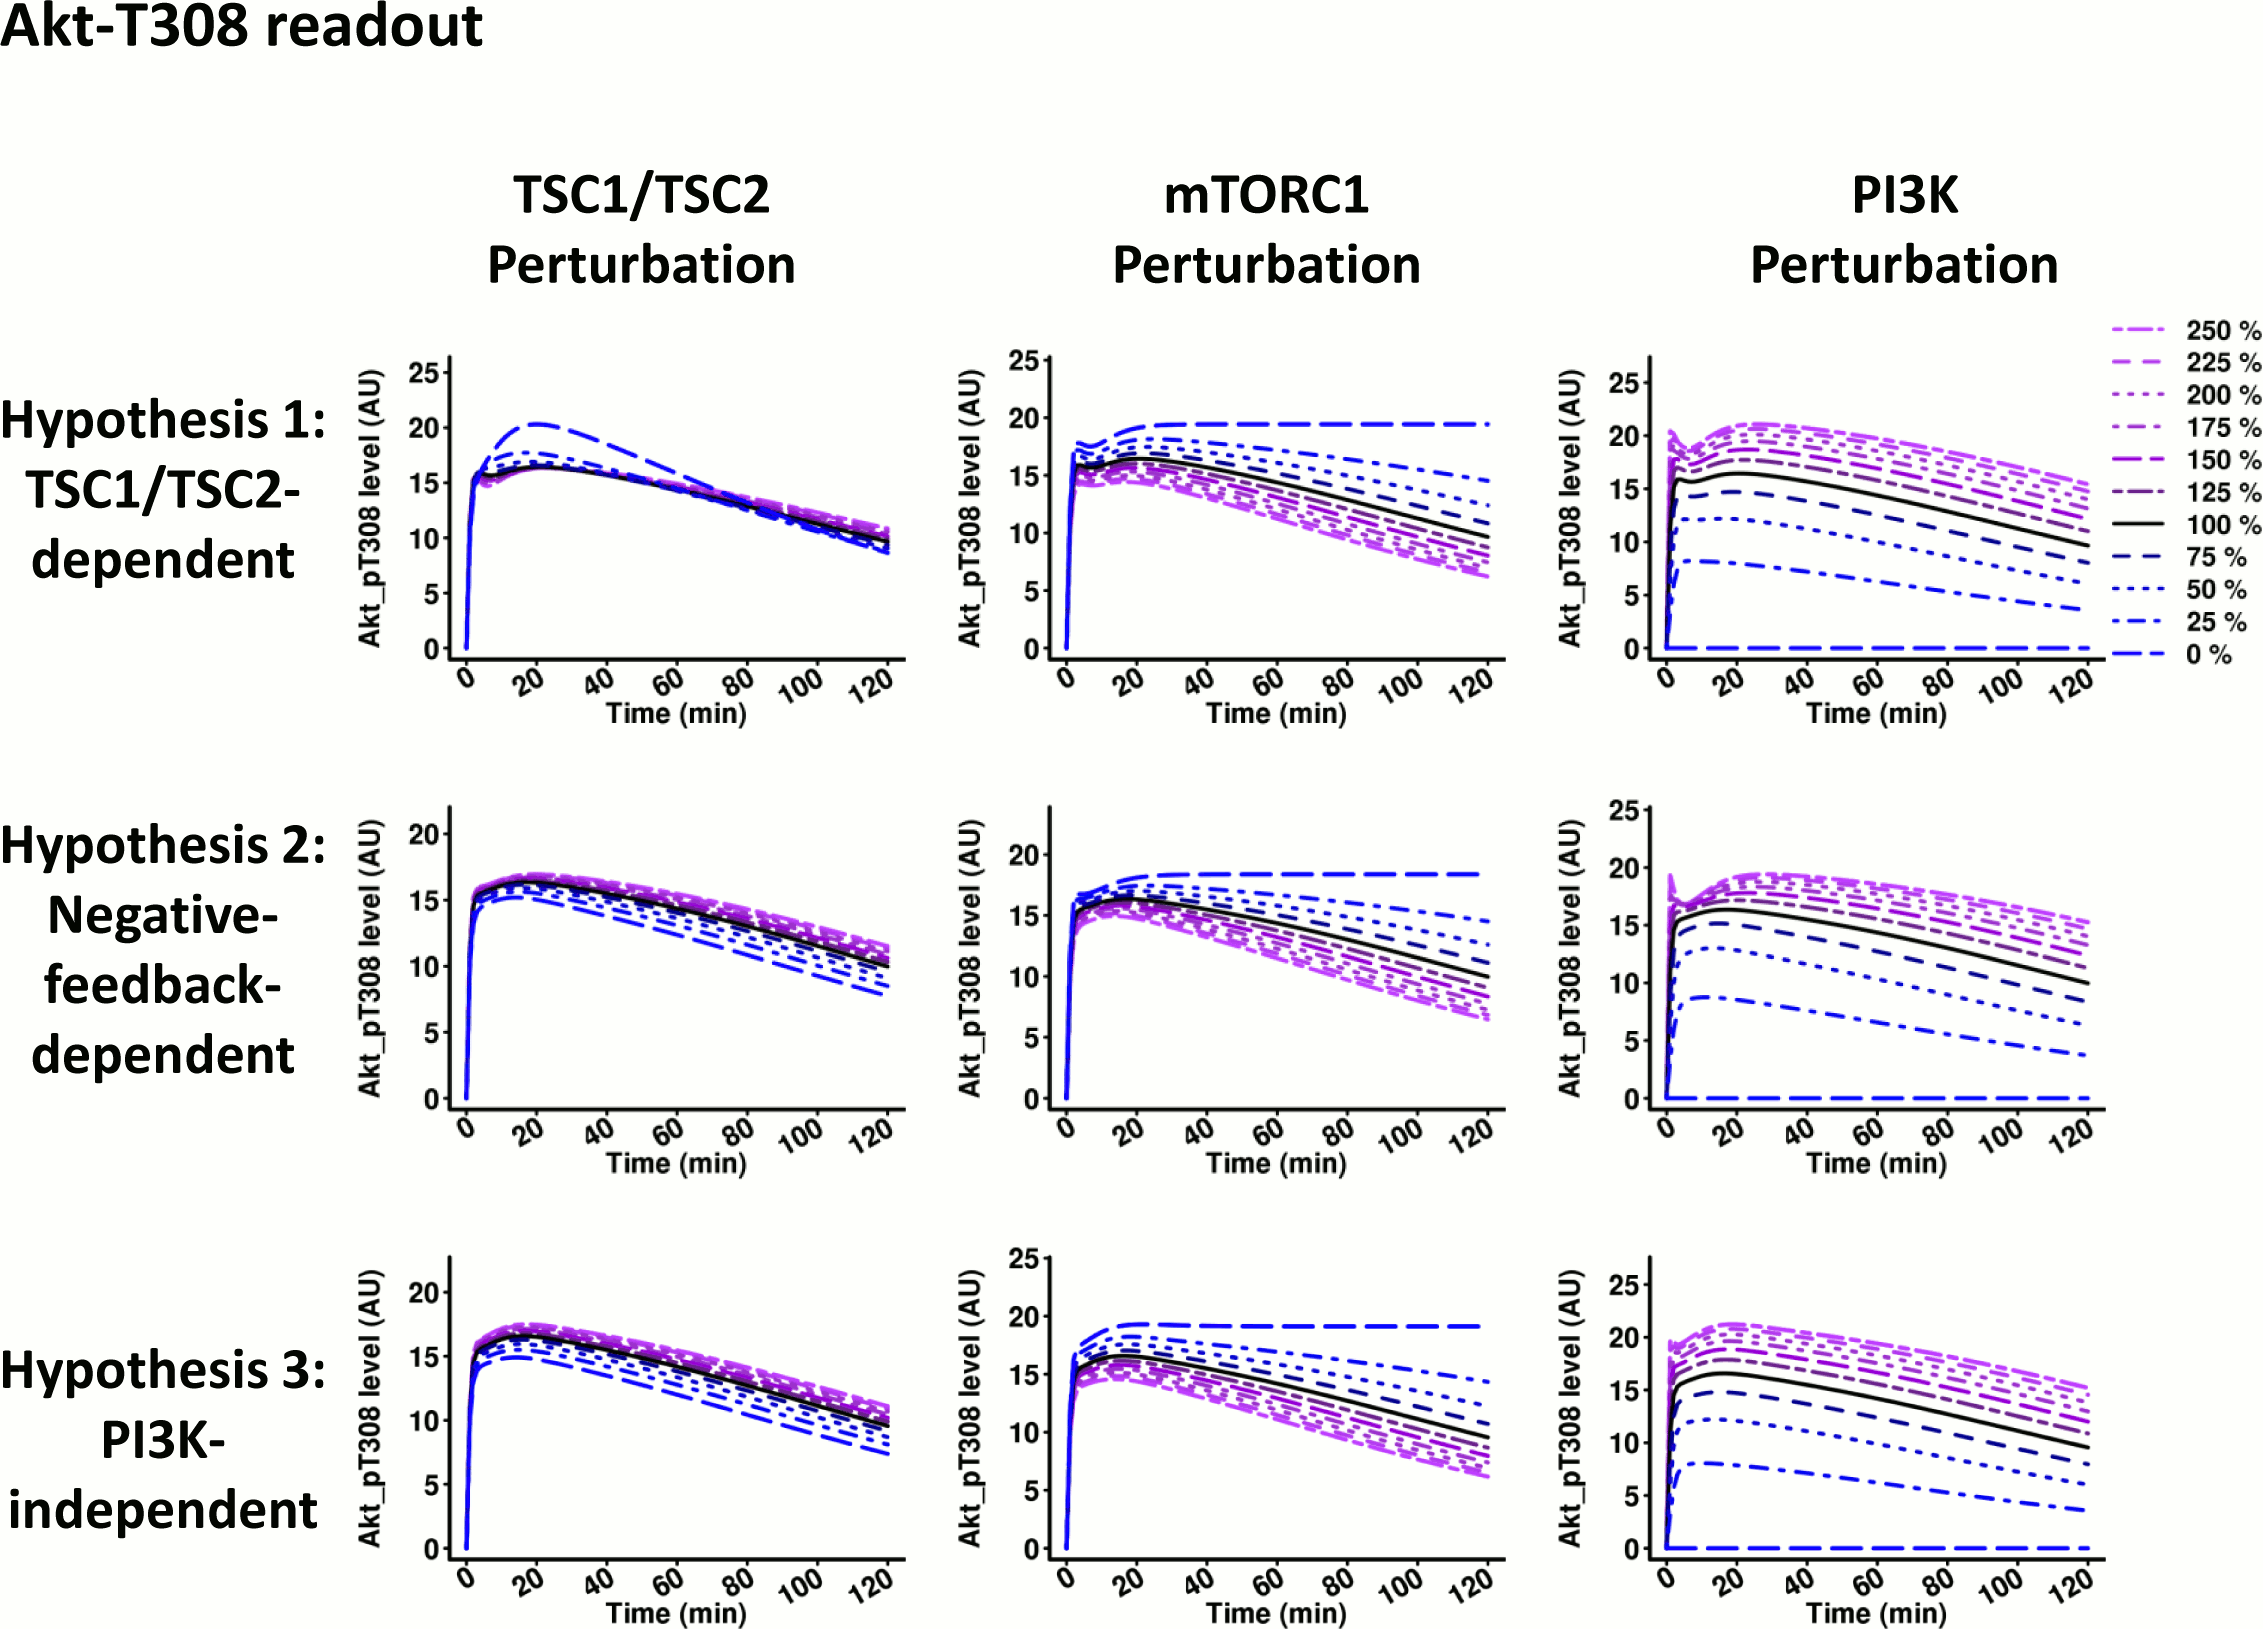
\includegraphics[scale=0.74]{2002469_supp_fig14.png}
		\caption[The influence of perturbations of TSC1/TSC2, mTORC1, or PI3K on the phosphorylation of Akt-T308 for the three hypotheses]{The influence of perturbations of TSC1/TSC2, mTORC1, or PI3K on the phosphorylation of Akt-T308 for the three hypotheses. The three hypotheses did not show any difference in the dynamics of Akt-T308 phosphorylation when varying the amounts of PI3K and mTORC1. A small difference was observed for TSC1/TSC2 perturbation where the TSC1/TSC2-dependent hypothesis showed a slight increase in Akt-T308 phosphorylation when TSC1/TSC2 activity was reduced. In the TSC1/TSC2-dependent hypothesis, the mTORC2 activity is reduced when the amount of TSC1/TSC2 is reduced.}
		\label{fig:2002469_supp_fig14}
	\end{center}
\end{figure}
\clearpage

\begin{figure}[tb]
	\begin{center}
		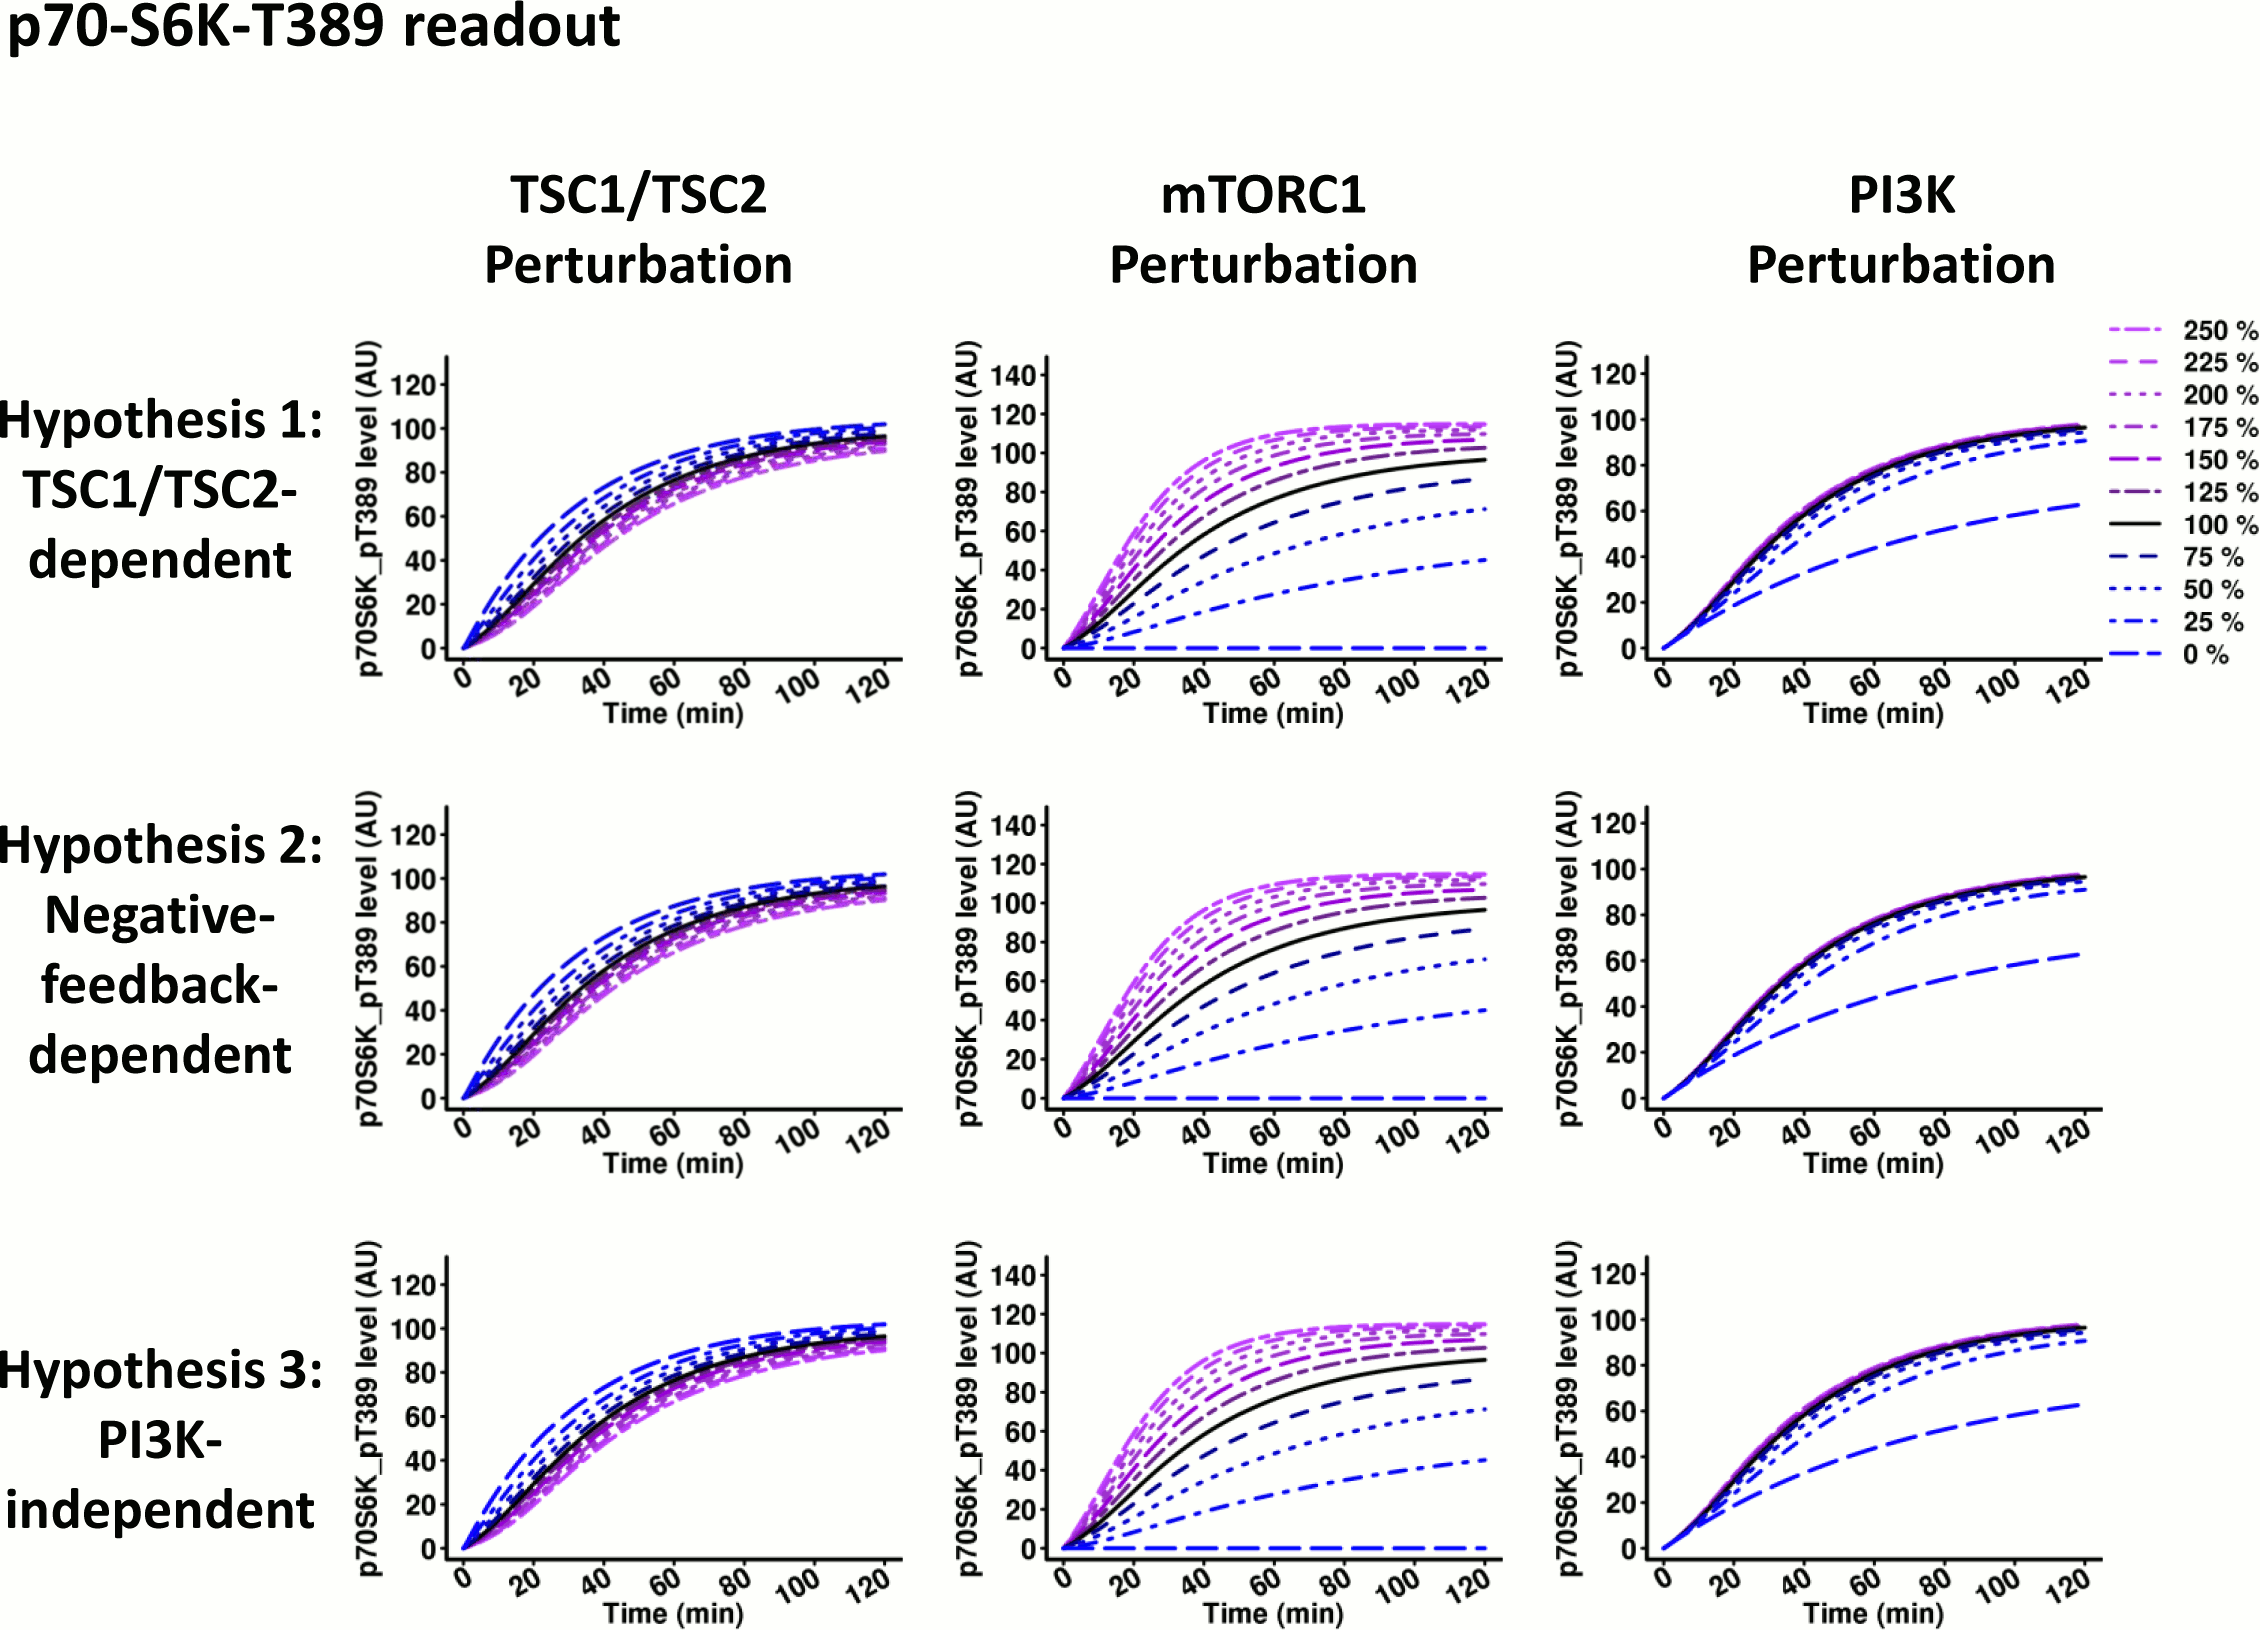
\includegraphics[scale=0.74]{2002469_supp_fig15.png}
		\caption[The influence of perturbations of TSC1/TSC2, mTORC1, or PI3K on the phosphorylation of p70-S6K-T389 for the three hypotheses]{The influence of perturbations of TSC1/TSC2, mTORC1, or PI3K on the phosphorylation of p70-S6K-T389 for the three hypotheses. The effect of each perturbation on the networks representing each hypothesis for the phosphorylation of p70-S6K-T389, which is a readout for mTORC1 activity, is shown.}
		\label{fig:2002469_supp_fig15}
	\end{center}
\end{figure}
\clearpage

\begin{figure}[tb]
	\begin{center}
		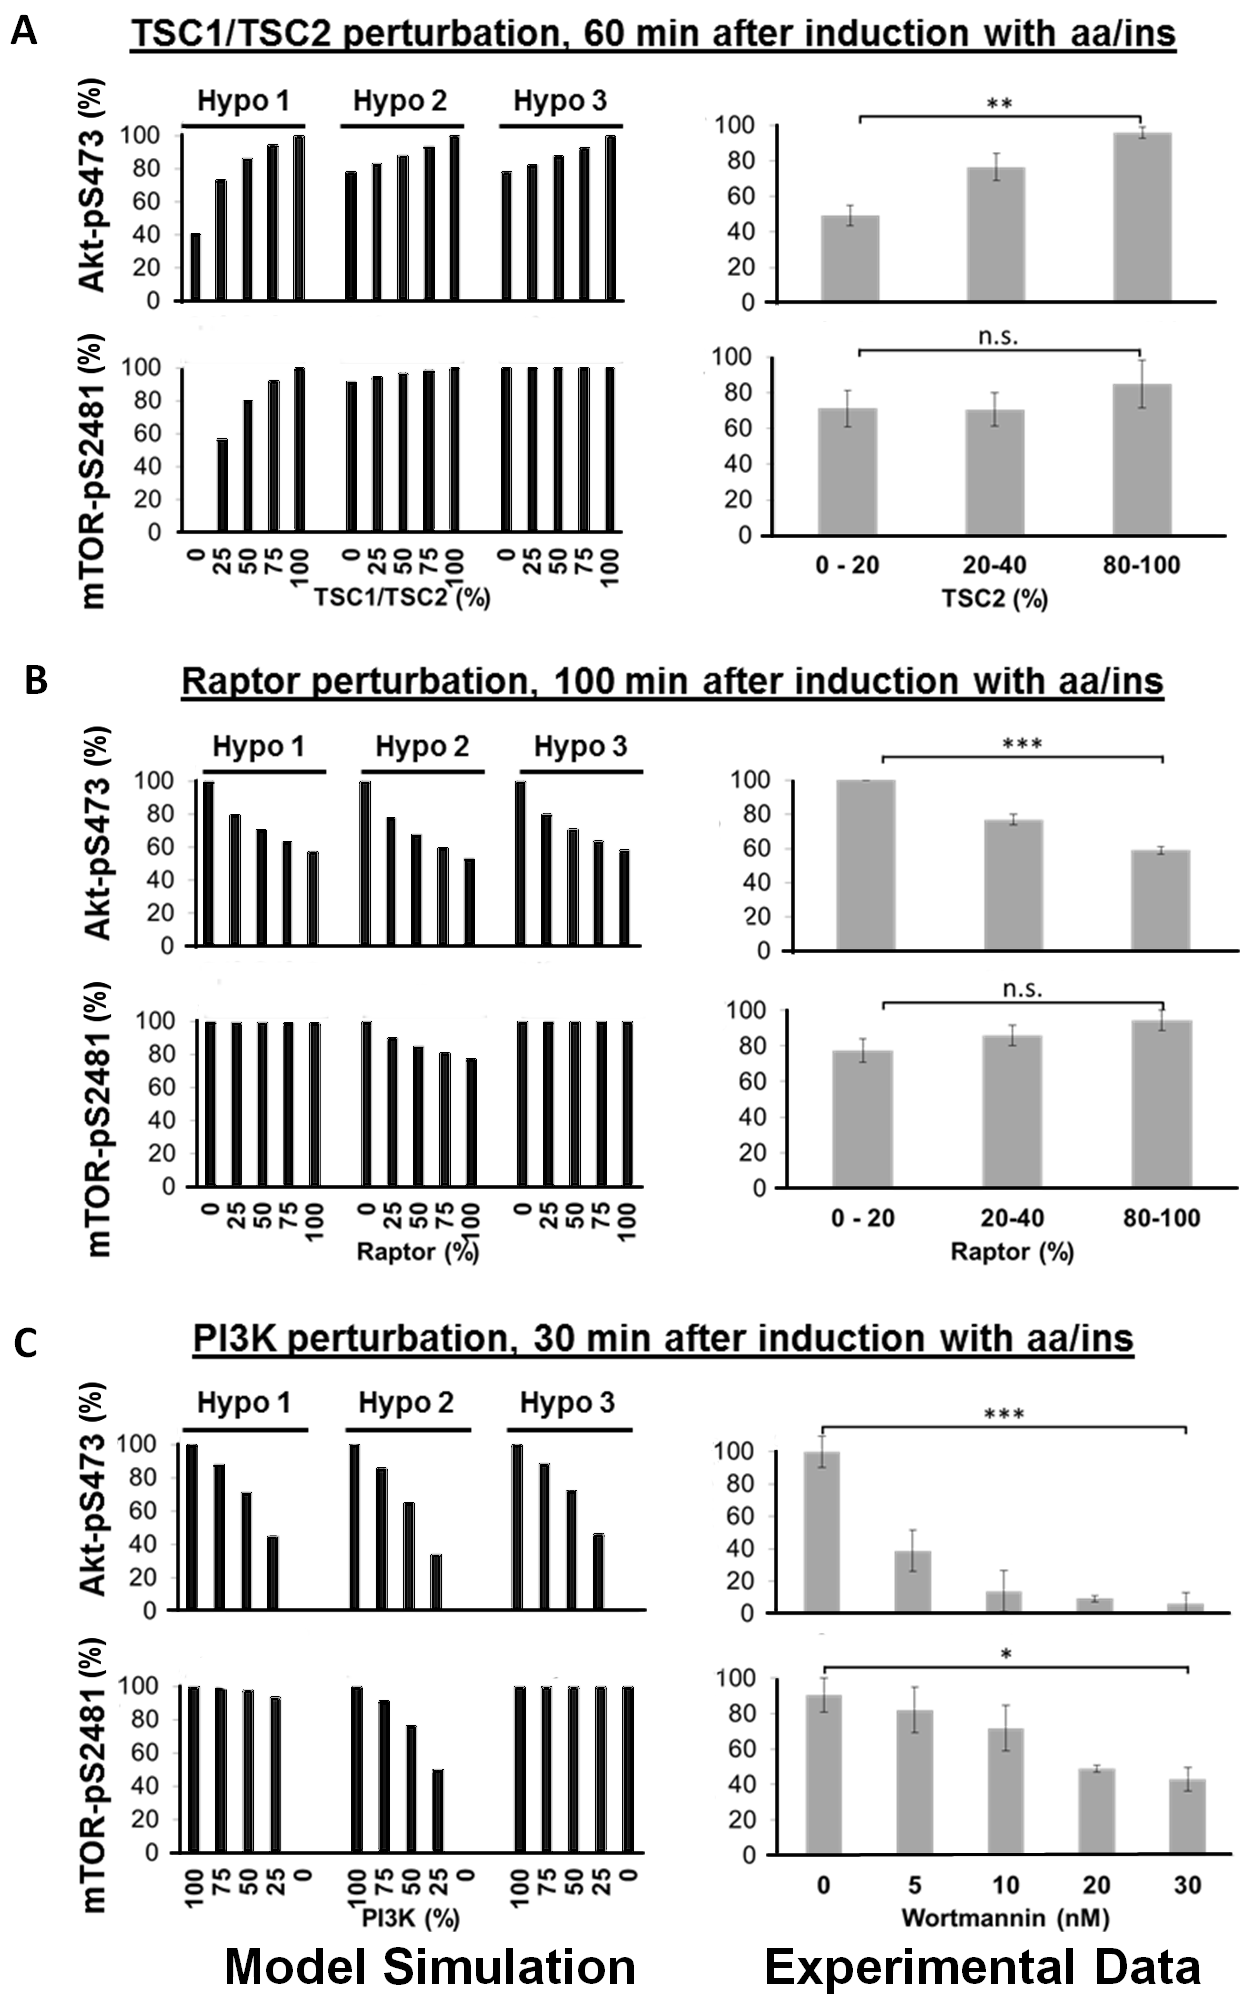
\includegraphics[width=4.0in]{2002469_fig678.png}
		%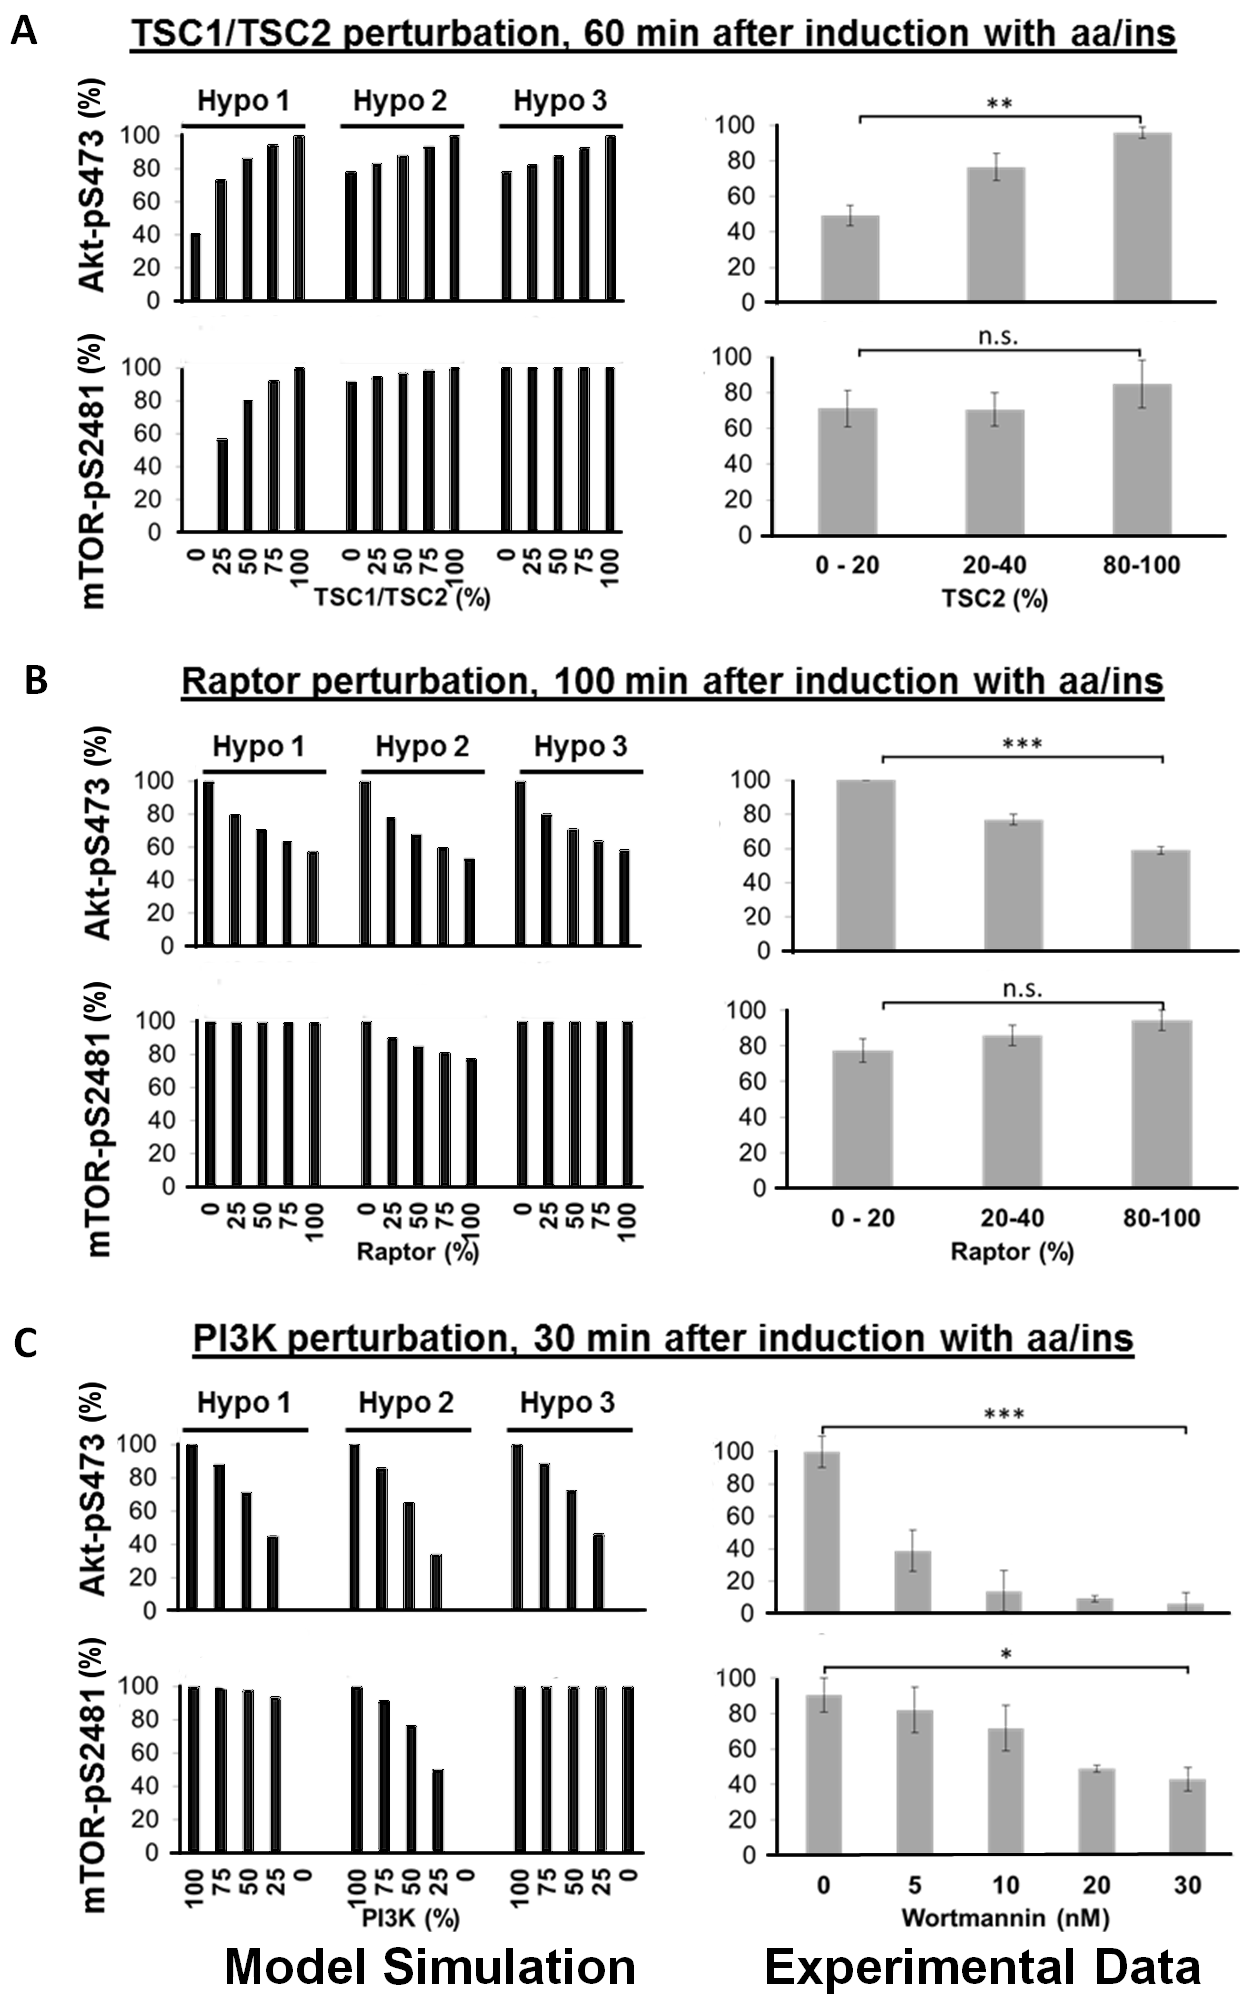
\includegraphics[scale=0.8]{2002469_fig678.png}
		\caption[Quantitative representations of simulated and experimentally determined Akt-pS473 and mTOR-pS2481]{Quantitative representations of simulated and experimentally determined Akt-pS473 and mTOR-pS2481. 
		(A) mTOR-pS2481 is not affected in response to a gradual TSC2 knock down for 60 min after induction with amino acids/insulin. 
		(B) mTOR-pS2481 is not affected by the NFL in response to Raptor knock down for 100 min after induction with amino acids/insulin. 
		(C) mTOR-pS2481 is sensitive to the PI3K inhibitor Wortmannin (Wmn) for 30 min after induction with amino acids/insulin. Data are the average and SEM computed from 3 repeats. * $P\;<\;0.05$, ** $P\;<\;0.01$, *** $P\;<\;0.001$, n.s. not significant. d = days, Hypo = hypothesis. \emph{In vitro} experiments were performed by Annika Sonntag, Freiburg University, Germany.}
		\label{fig:2002469_fig678}
	\end{center}
\end{figure}
\clearpage

\begin{figure}[tb]
	\begin{center}
		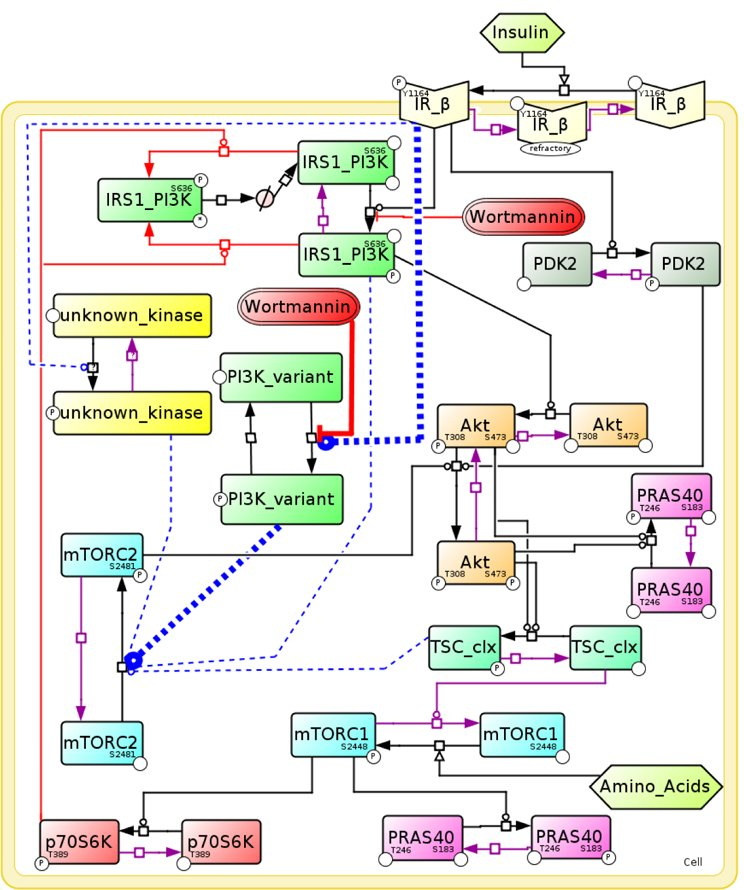
\includegraphics[scale=1.8]{2002469_fig9B.jpg}
		\caption[A new hypothesis and network structure for mTORC2 regulation by insulin]{A new hypothesis and network structure for mTORC2 regulation by insulin. Schematic representation of the pathway for Hypothesis 4: Insulin induction of mTORC2 by a PI3K (red) that is insensitive to TSC1/TSC2 and to the S6K to IRS-mediated NFL. This hypothesis was equivalent to Hypothesis 3 (PI3K and TSC1/TSC2-independent activation), assuming that the mTORC2 activator was sensitive to Wortmannin.}
		\label{fig:2002469_fig9B}
	\end{center}
\end{figure}

\clearpage
\begin{figure}[tb]
	\begin{center}
		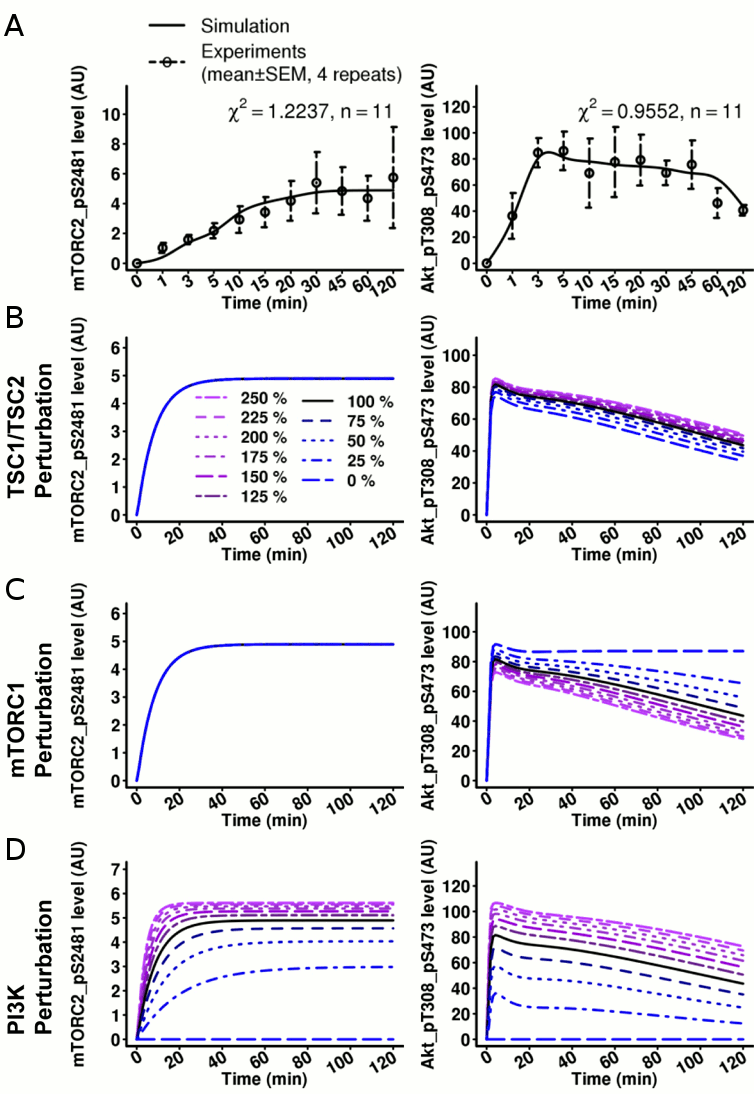
\includegraphics[scale=1.35]{2002469_fig9CF.png}
		\caption[A new hypothesis and network structure for mTORC2 regulation by insulin]{A new hypothesis and network structure for mTORC2 regulation by insulin. (A) The model simulation data for Hypothesis match the experimental dynamical phosphorylation data. The simulated and experimentally measured dynamics are shown for the mTORC2 readouts mTOR-pS2481 and Akt-pS473 (see Figure \ref{fig:2002469_supp_fig16} for all other readouts). (B) Predictions for mTOR-pS2481 and Akt-pS473 upon gradual TSC1/TSC2 knock down match the experimental data, which is presented in Figure \ref{fig:2002469_fig678}A. Whereas at 60 min after induction Akt-pS473 is gradually reduced by TSC2 inhibition, mTOR-pS2481 is TSC2-insensitive. See Figure \ref{fig:2002469_supp_fig16} for Akt-pT308 and p70-S6K-pT389. (C) Predictions for mTOR-pS2481 and Akt-pS473 readouts upon gradual Raptor knock down match the experimental data, which is presented in Figure \ref{fig:2002469_fig678}B. Whereas at 100 min after induction Akt-pS473 is gradually 
induced by Raptor inhibition, mTOR-pS2481 is Raptor-insensitive. See Figure \ref{fig:2002469_supp_fig16} for Akt-pT308 and p70-S6K-pT389. (D) Predictions for mTOR-pS2481 and Akt-pS473 readouts upon gradual PI3K inhibition match the experimental data, which is presented in Figure \ref{fig:2002469_fig678}C. Both Akt-pS473 and mTOR-pS2481 are gradually reduced by Wortmannin at 30 min after induction. See Figure \ref{fig:2002469_supp_fig16} for Akt-pT308 and p70-S6K-pT389. \emph{In vitro} experiments were performed by Annika Sonntag, Freiburg University, Germany.}
		\label{fig:2002469_fig9CF}
	\end{center}
\end{figure}
\clearpage

\begin{figure}[tb]
	\begin{center}
		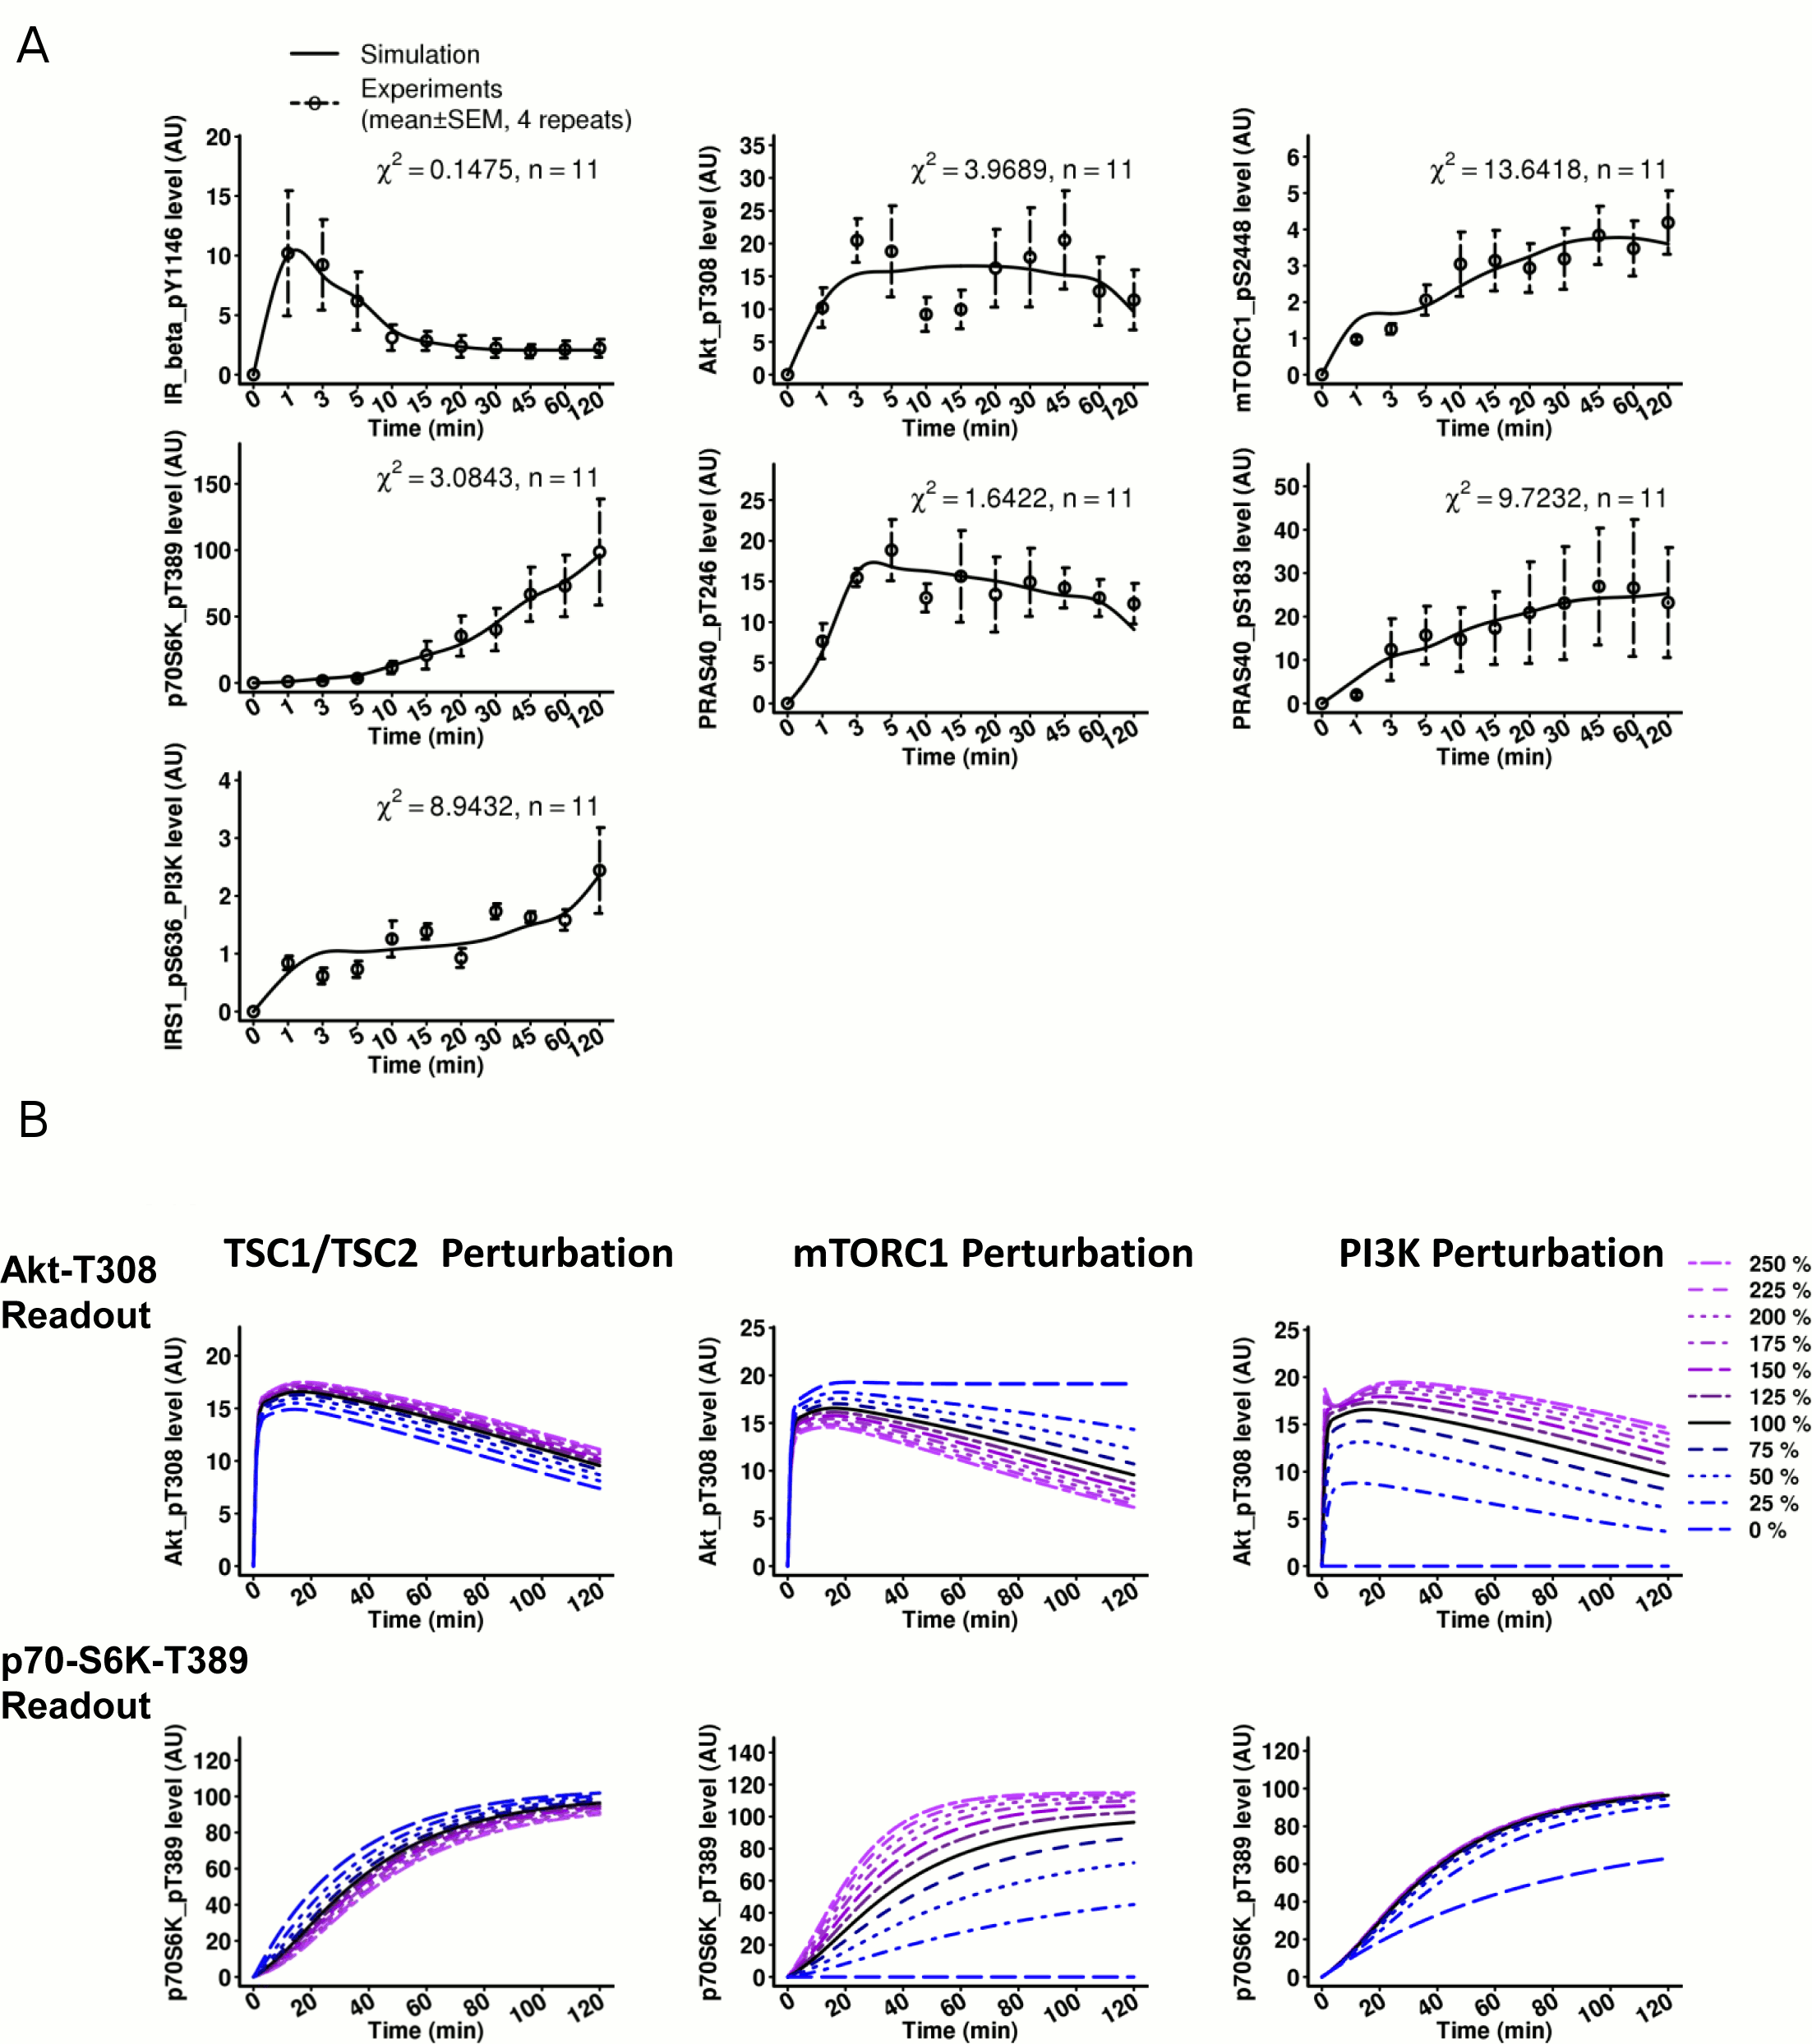
\includegraphics[scale=0.75]{2002469_supp_fig16.png}
		\caption[Simulation and perturbations for the new network structure based on Hypothesis 4: PI3K-dependent, NFL-independent regulation of mTORC2]{Simulation and perturbations for the new network structure based on Hypothesis 4: PI3K-dependent, NFL-independent regulation of mTORC2. (A) Comparison between the simulated and experimental time courses for Hypothesis 4 shows that the simulated time courses match the experimental readouts. (B) The influence of perturbations of TSC1/TSC2, mTORC1, or PI3K on the dynamics of phosphorylation of Akt-T308 and p70-S6K-T389 for Hypothesis 4. \emph{In vitro} experiments were performed by Annika Sonntag, Freiburg University, Germany.}
		\label{fig:2002469_supp_fig16}
	\end{center}
\end{figure}
\clearpage

\begin{figure}[tb]
	\begin{center}
		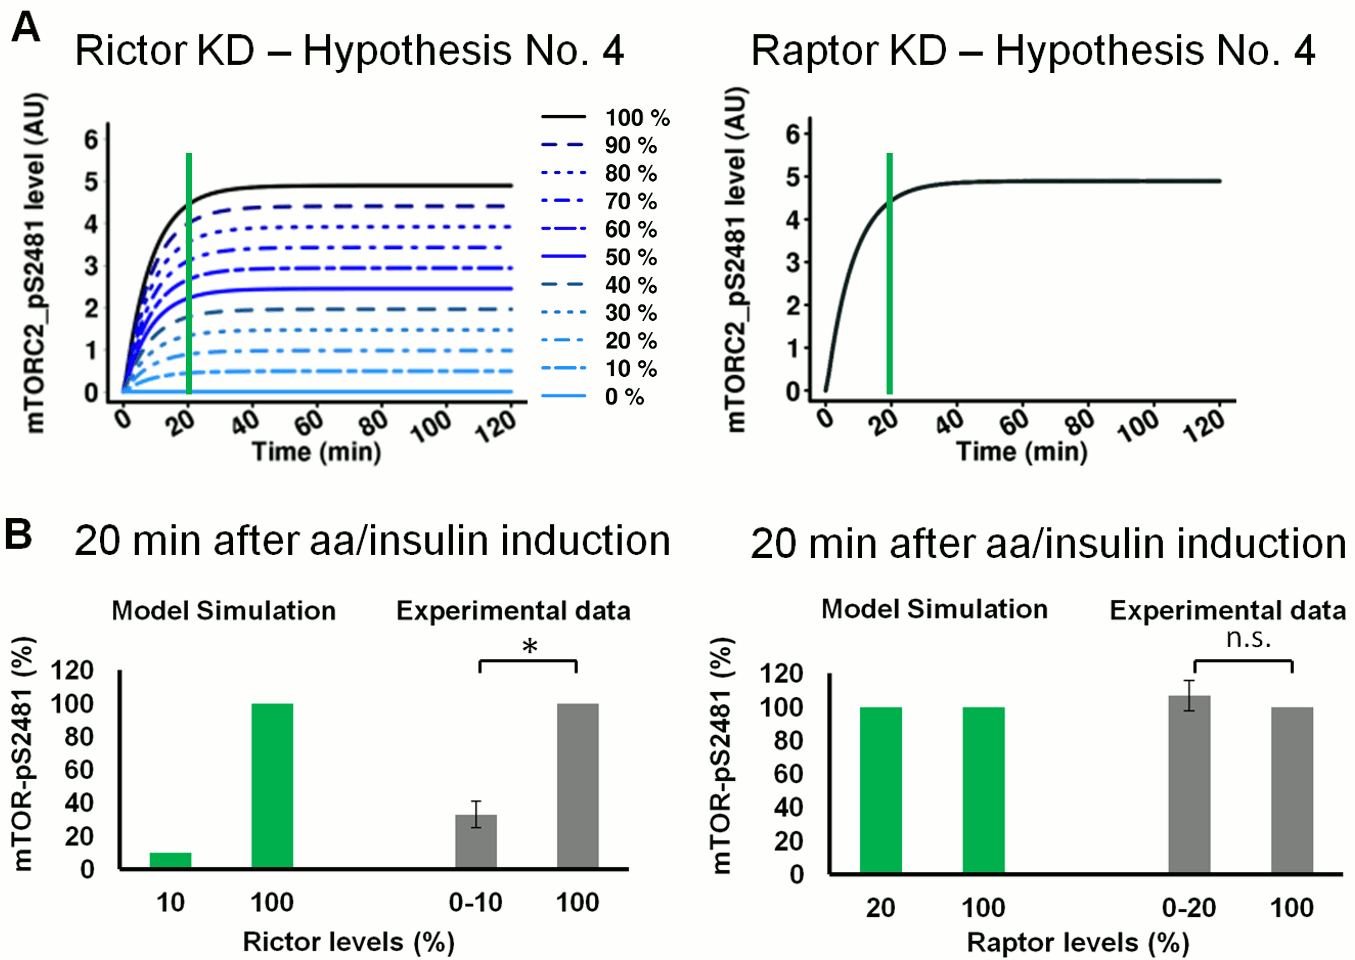
\includegraphics[scale=1]{response_letter_fig1.png}
		\caption[Validation Hypothesis 4 by Rictor and Raptor knock down.]{Validation Hypothesis 4 by Rictor and Raptor knock down. (A) Simulation of mTOR-pS2481 dynamic in response to addition of amino acids and insulin when Rictor or Raptor is knocked down (KD). (B) Quantifications of the simulations and experimental data for mTOR-pS2481 upon Rictor or Raptor knock down 20 min after amino acids/insulin induction. * $P\;<\;0.01$; n.s., not significant; Student's $t$-test. \emph{In vitro} experiments were performed by Annika Sonntag, Freiburg University, Germany. (See \citep[Fig. 1]{DallePezze2012b}).}
		\label{fig:response_letter_fig1}
	\end{center}
\end{figure}
\clearpage

\begin{figure}[tb]
	\begin{center}
		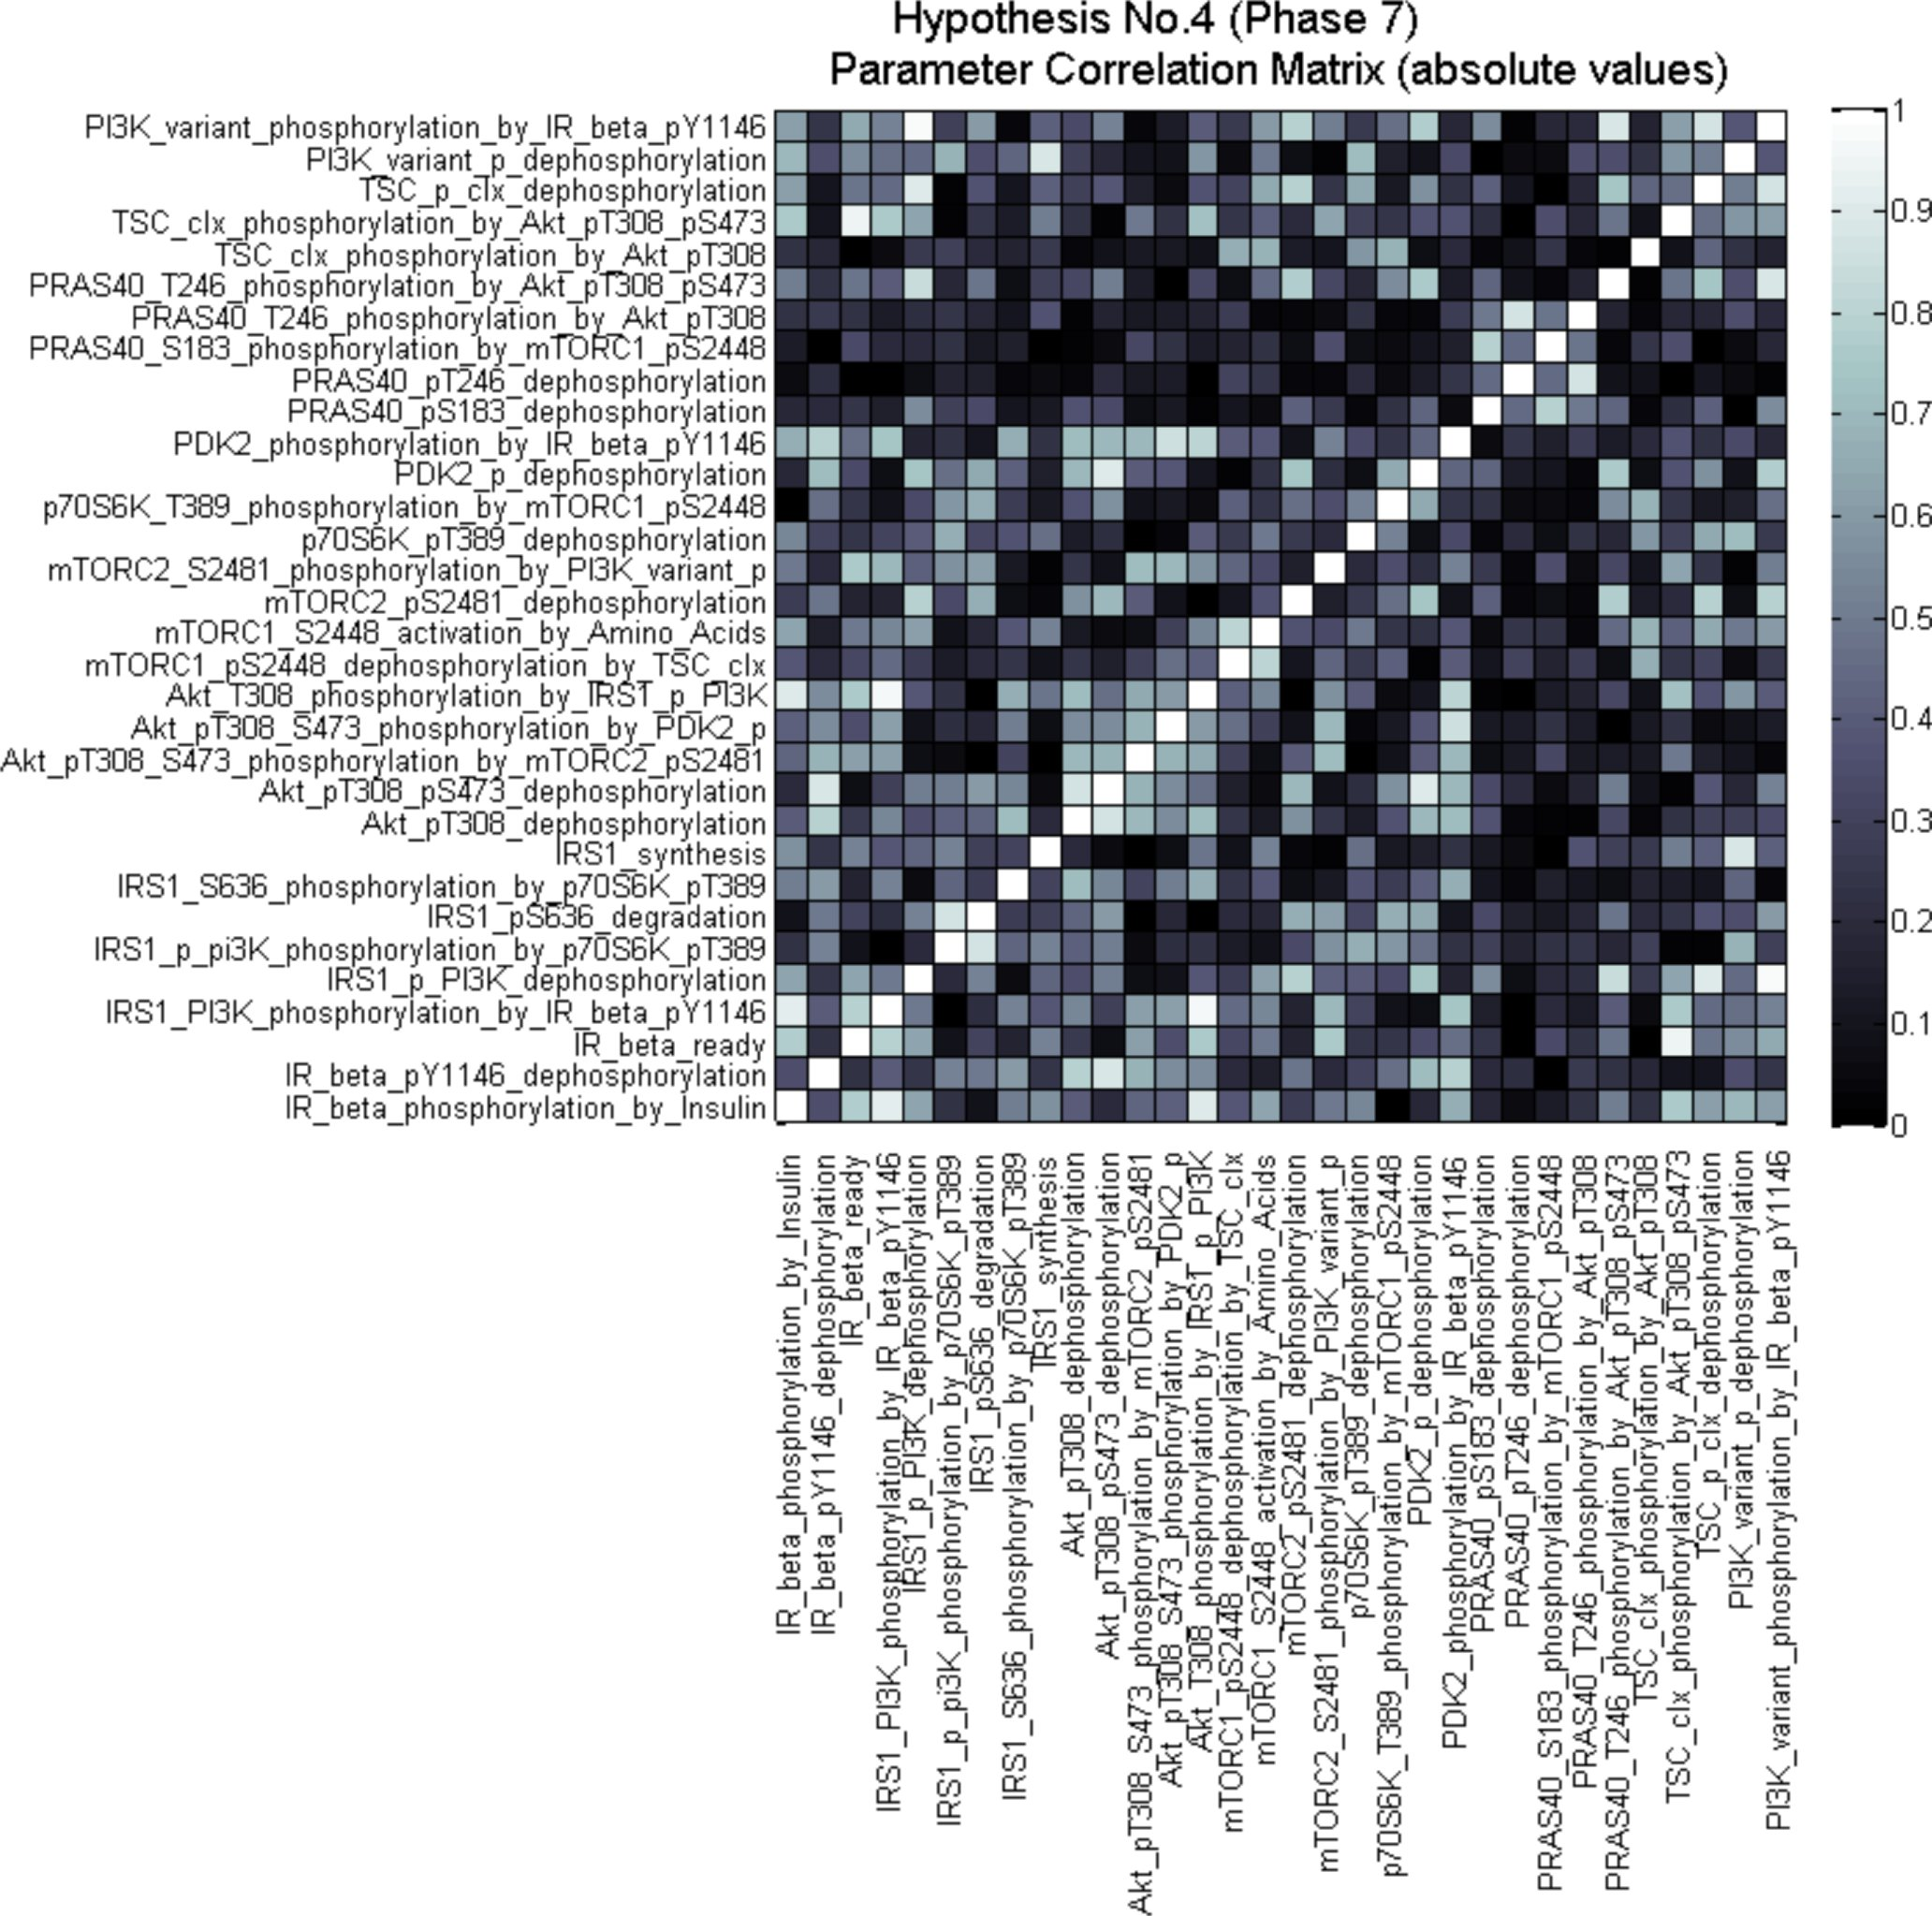
\includegraphics[scale=0.8]{2002469_supp_fig17.jpg}
		\caption[Identifiability analysis for Hypothesis 4: PI3K-dependent, NFL-independent regulation of mTORC2]{Identifiability analysis for Hypothesis 4: PI3K-dependent, NFL-independent regulation of mTORC2. Parameter correlation matrix for Hypothesis 4 is shown. See Figure \ref{fig:2002469_supp_fig5} for details.}
		\label{fig:2002469_supp_fig17}
	\end{center}
\end{figure}
\clearpage

\begin{figure}[tb]
	\begin{center}
		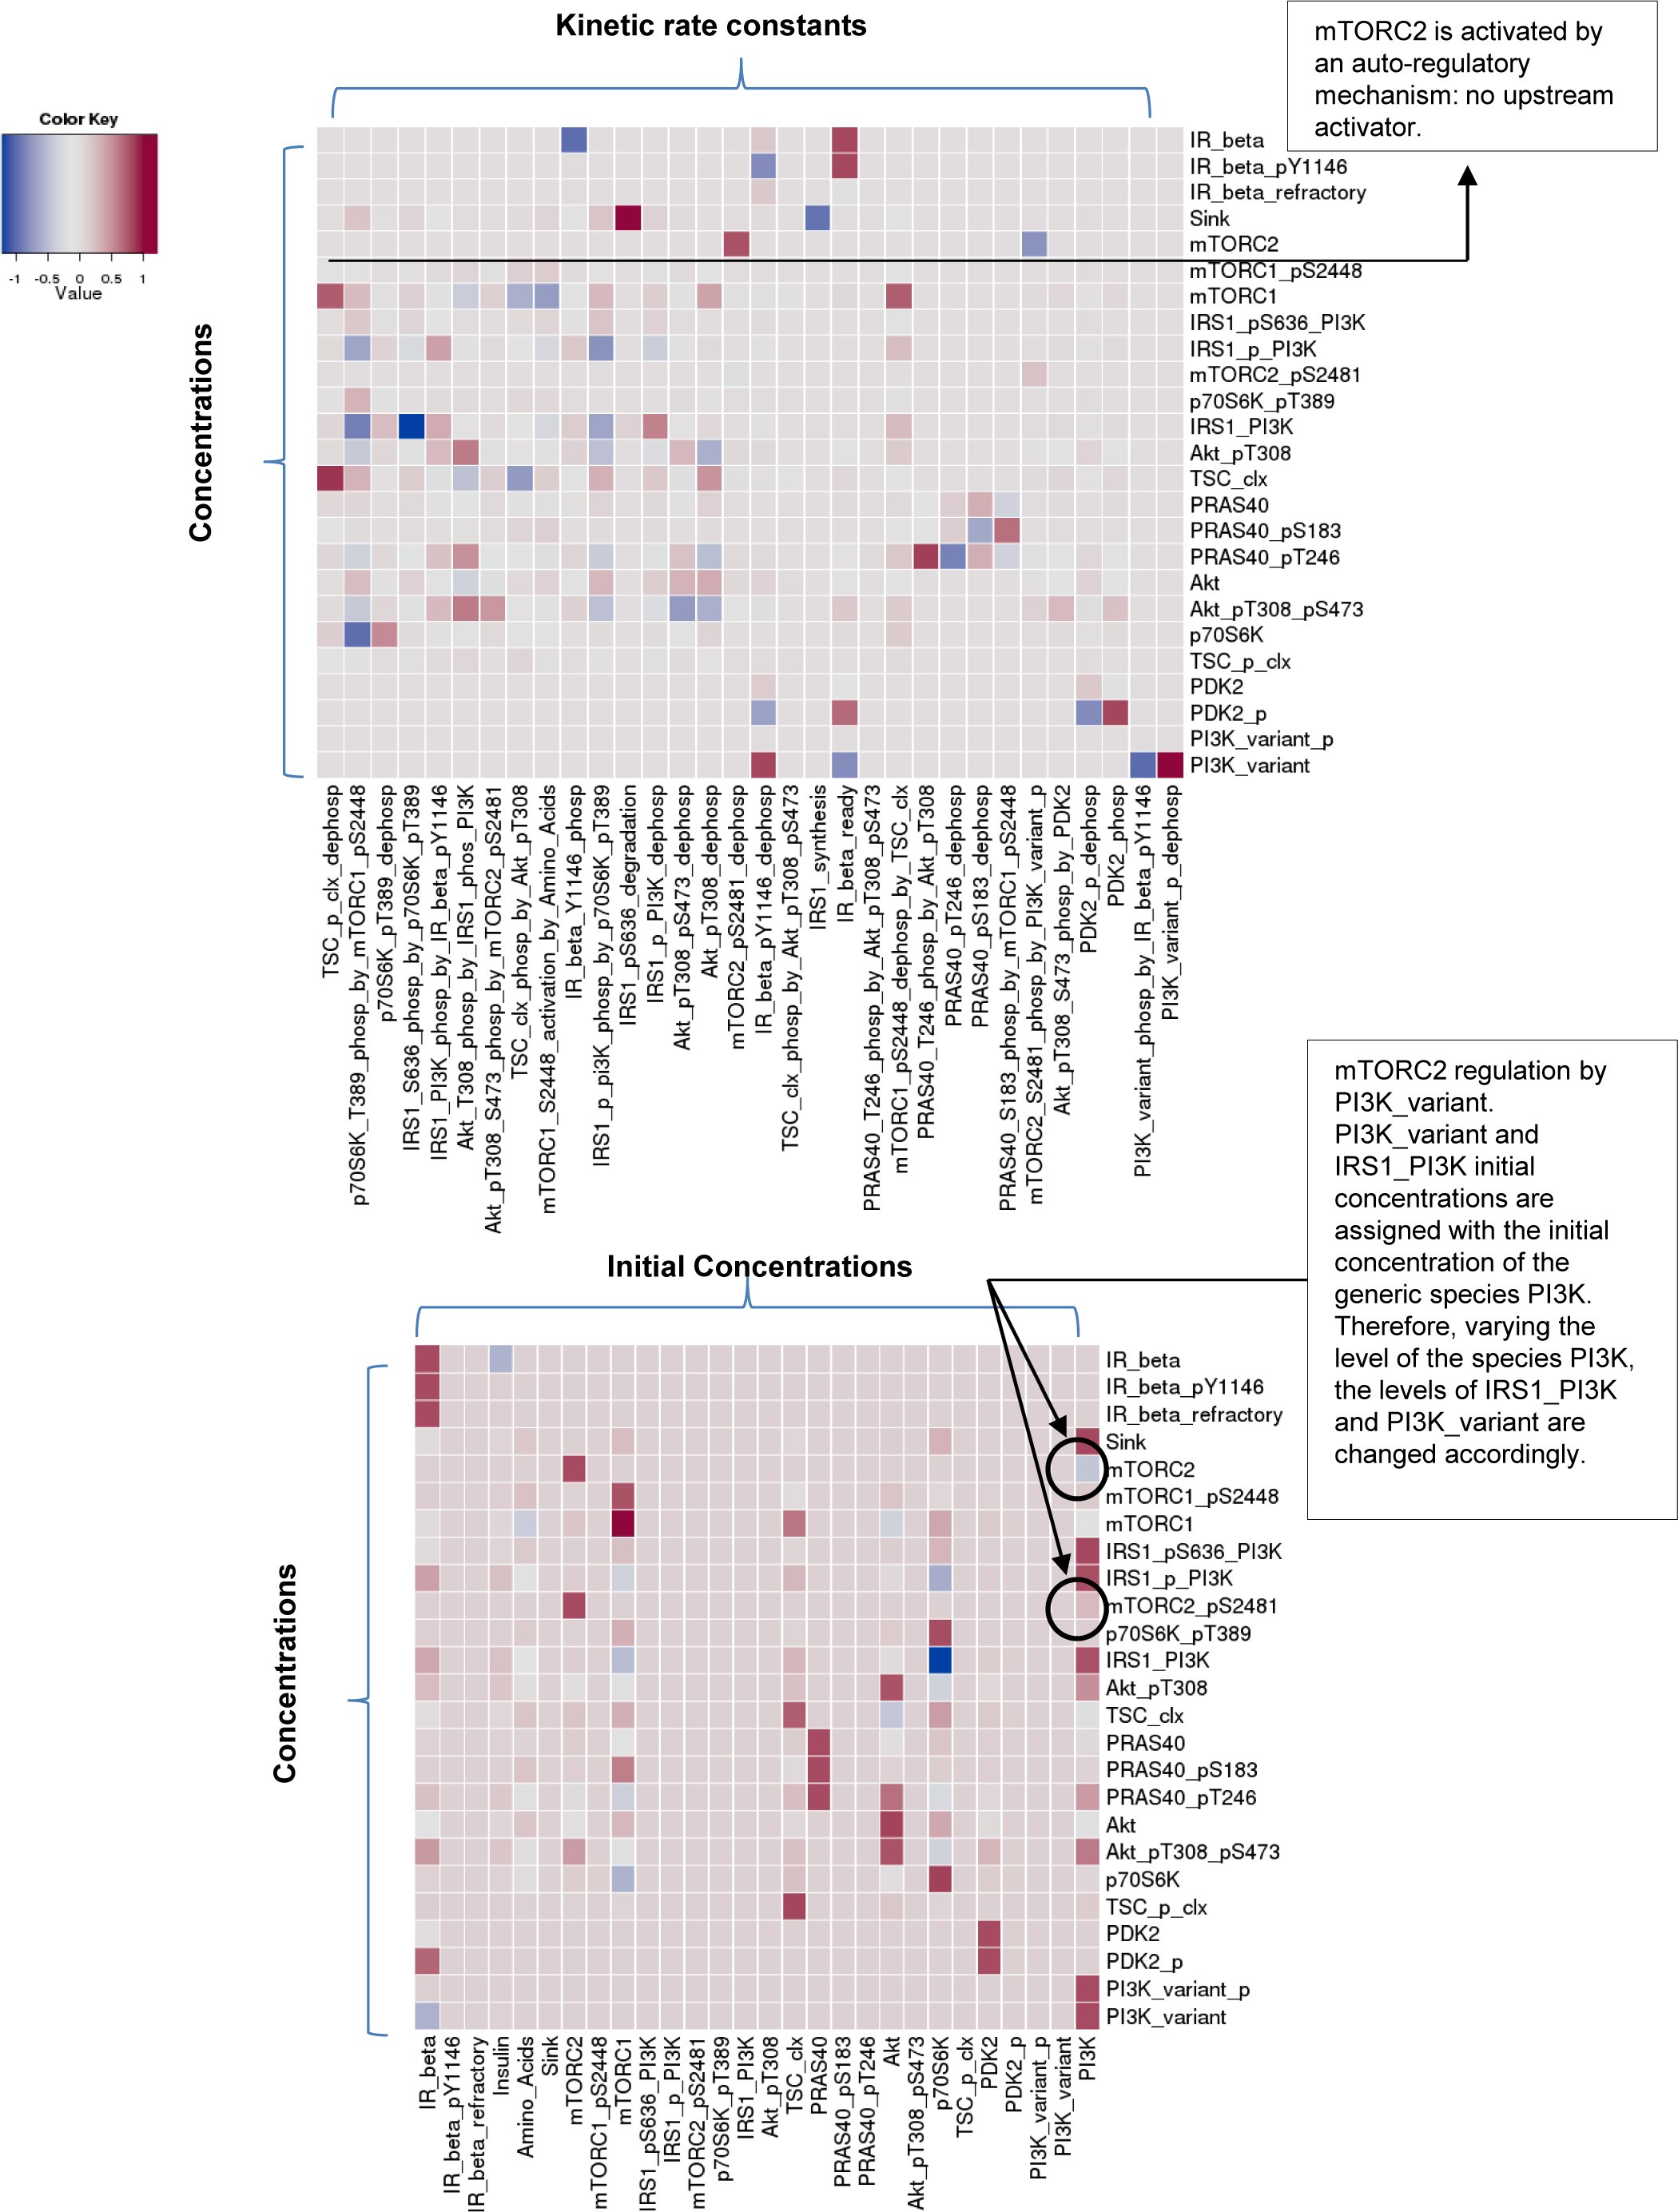
\includegraphics[scale=0.75]{2002469_supp_fig18.jpg}
		\caption[Sensitivity analysis for Hypothesis 4: PI3K-dependent, NFL-independent regulation of mTORC2]{Sensitivity analysis for Hypothesis 4: PI3K-dependent, NFL-independent regulation of mTORC2. Sensitivity analysis for the initial concentrations and the kinetic rates parameters for Hypothesis 4 is shown. See Figure \ref{fig:2002469_supp_fig6} for details of the top and bottom plots.}
		\label{fig:2002469_supp_fig18}
	\end{center}
\end{figure}
\clearpage






%\section{Tables}
%\label{paper1-sec:Tables}

\begin{table}[tb]
	\begin{center}
		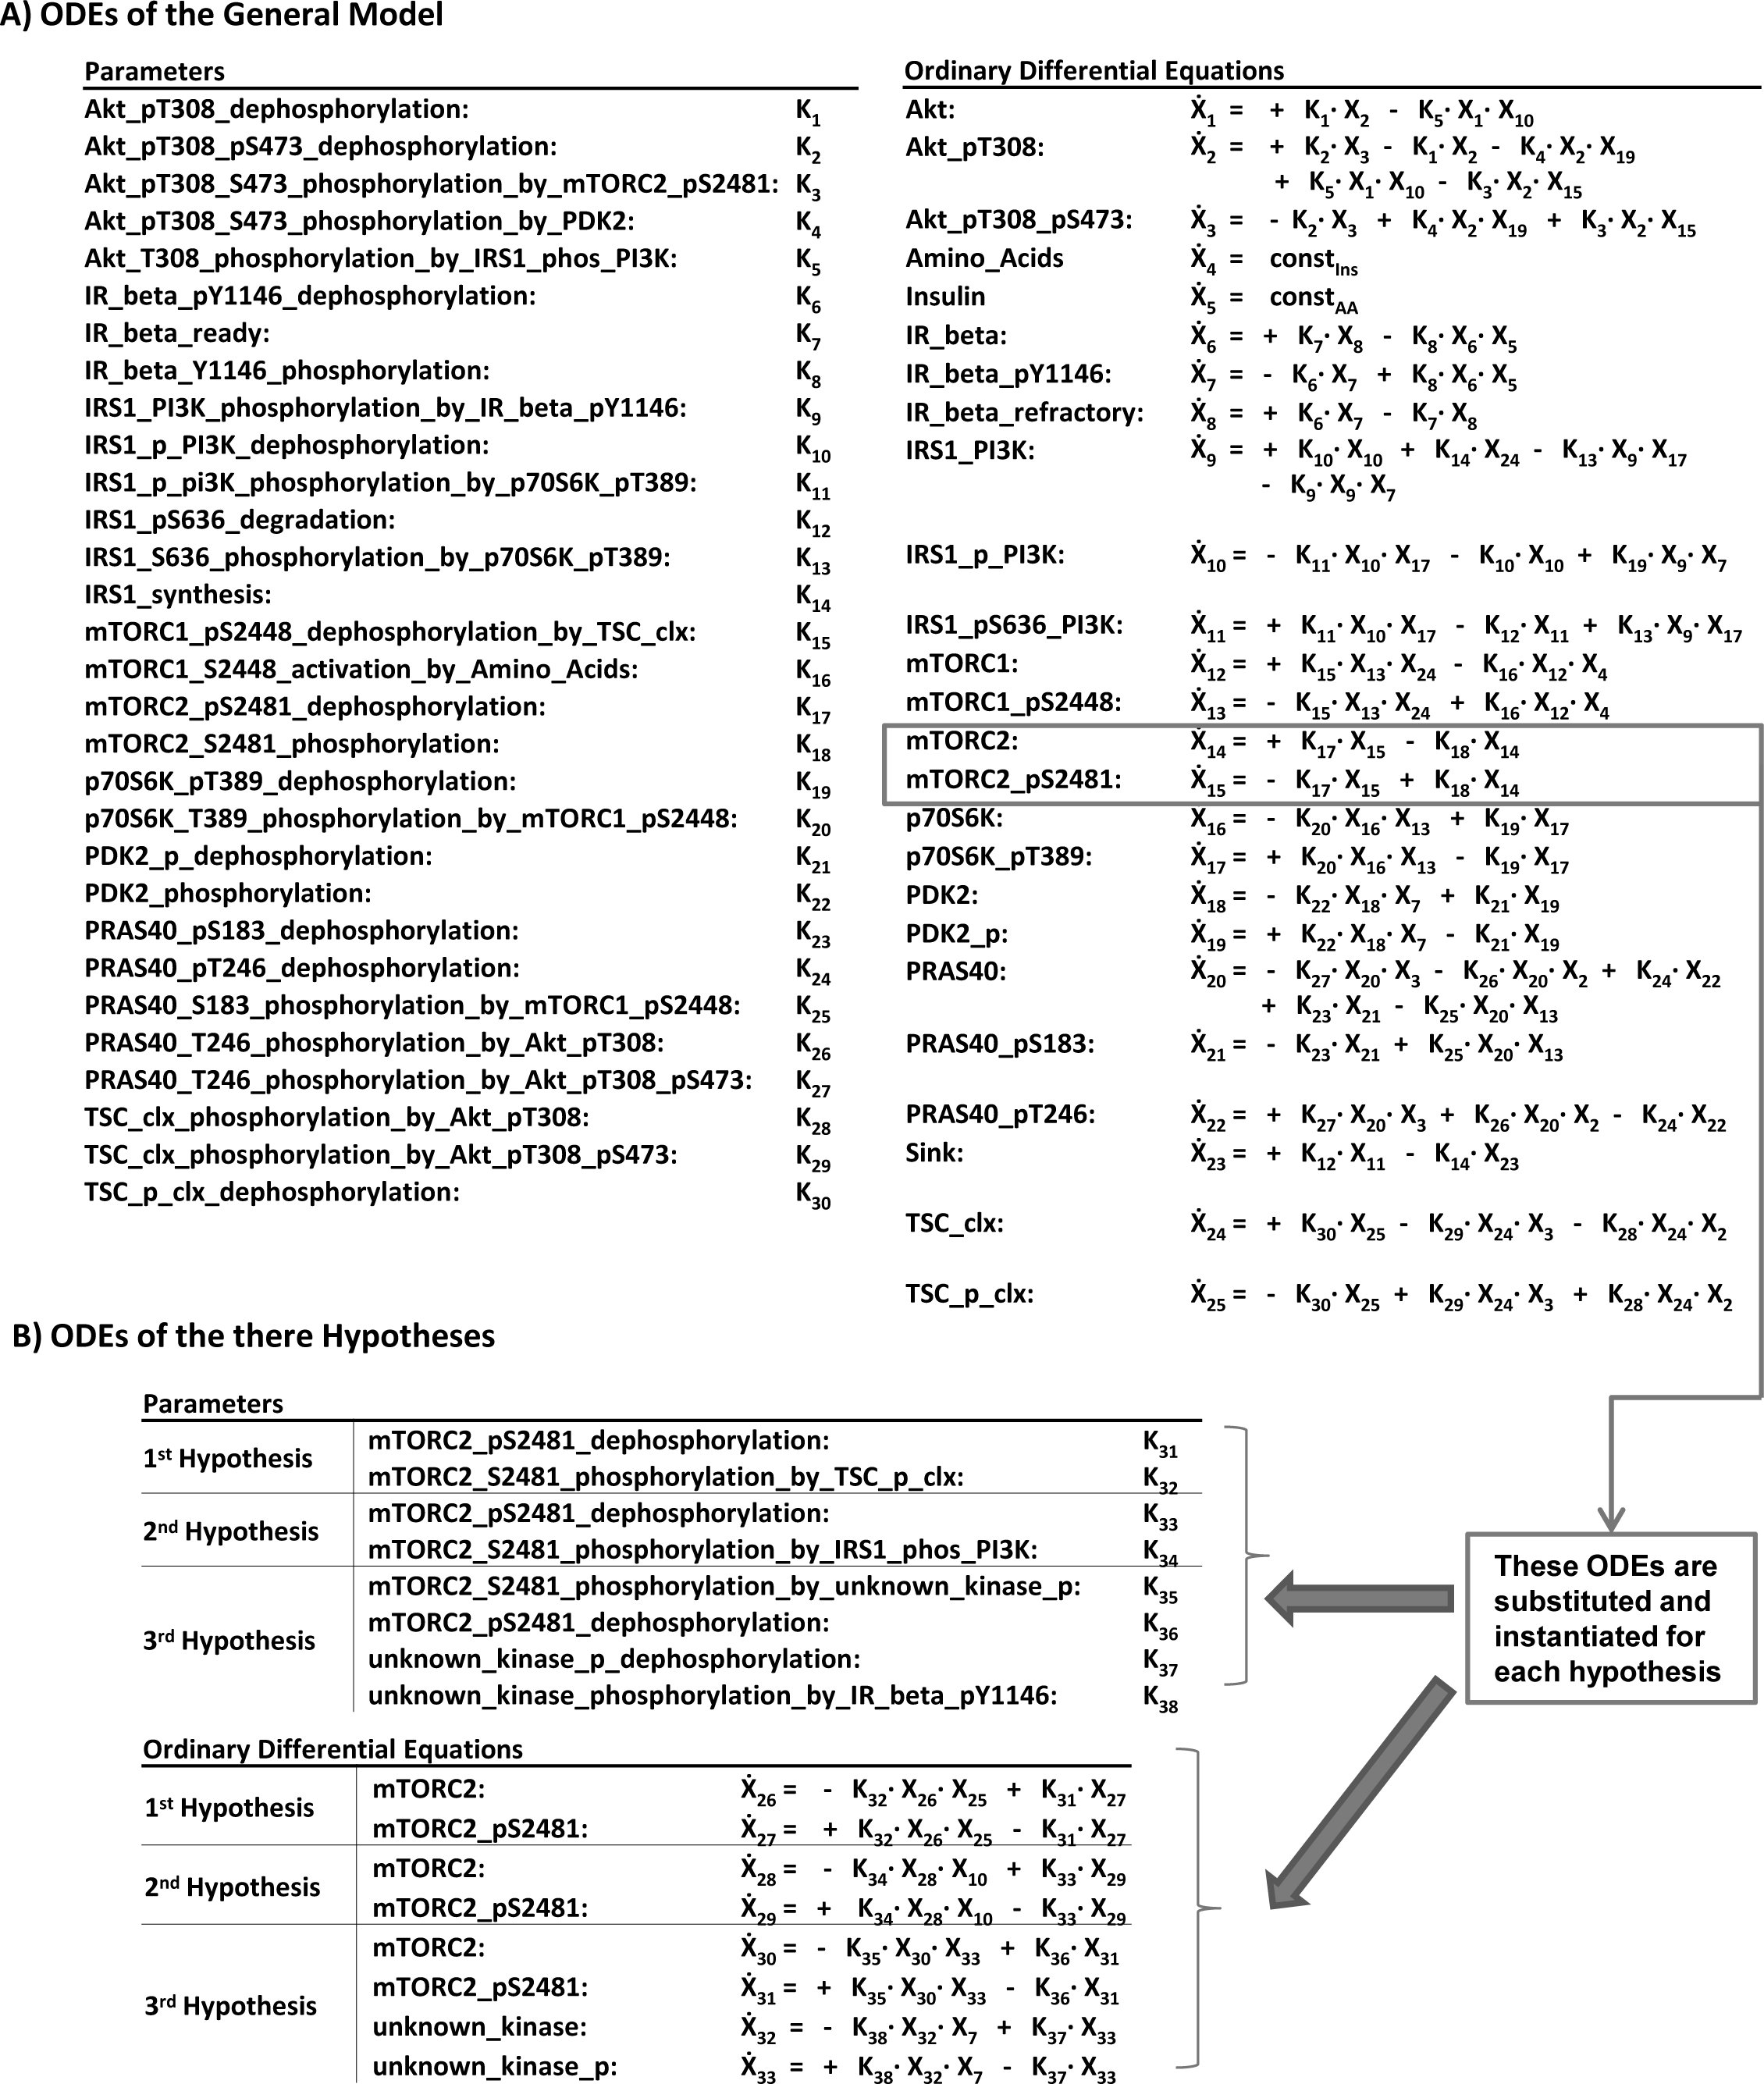
\includegraphics[scale=0.75]{2002469_supp_tab1.png}
		\caption[Ordinary differential equations of the general model and the models representing Hypothesis 1, 2, and 3 for mTORC2 activation]{Ordinary differential equations of the general model and the models representing Hypothesis 1, 2, and 3 for mTORC2 activation. List of kinetic rate constants and ordinary differential equations (ODEs) for the general model (A) and the Hypotheses 1, 2, and 3 (B). Each hypothesis is derived from the general model by replacing the mTORC2 ODEs, shown in the box, with those corresponding to the hypothesis.}
		\label{tab:2002469_supp_tab1}
	\end{center}
\end{table}
\clearpage

\begin{table}[tb]
	\begin{center}
		\includegraphics[scale=0.72]{2002469_supp_tab2.png}
		\caption[Parameter values of the general model]{Parameter values of the general model. The general model was fully parameterised by three steps. Phase 1, 3 kinetic rate constants of the insulin receptor (IR-beta) were determined. Phase 2, the general model without PDK2 was obtained by parameterising 24 kinetic rate constants. In this phase, Akt-S473 activation is modelled as autoregulation, independent of mTORC2 and PDK2. Phase 3, PDK2 dynamics were added to the system and the 3 parameters regulating Akt-S473 phosphorylation were calibrated by substituting the previously introduced autoregulatory mechanism (parameters values shown in red) of Akt. For each phase, 350 independent calibrations, starting from random initial configurations of the parameters, were executed and the best solution set fitting the data was selected. Phase 1 and 3 converged to a single solution set. Phase 2 converged to two solutions sets of which one was discarded as inconsistent with the experimental data (shown for phosphorylated 
Akt-S473 and IRS1-S636 readouts). For each phase, the mean and standard deviation of the estimated parameters were computed from the selected solution set. The solution closest to the centroid of the selected solution cluster was chosen for fixing the parameter values. \emph{In vitro} experiments were performed by Annika Sonntag, Freiburg University, Germany.}
		\label{tab:2002469_supp_tab2}
	\end{center}
\end{table}
\clearpage

\begin{table}[tb]
	\begin{center}
		\includegraphics[scale=0.75]{2002469_supp_tab3.png}
		\caption[Parameter values of Hypotheses 1, 2, and 3]{Parameter values of Hypotheses 1, 2, and 3. For each hypothesis, the estimated parameters were calibrated using the same protocol provided in Table \ref{tab:2002469_supp_tab2}. For each hypothesis, all the corresponding calibrations converged to a single solution set.}
		\label{tab:2002469_supp_tab3}
	\end{center}
\end{table}
\clearpage

\begin{table}[tb]
	\begin{center}
		\includegraphics[scale=0.75]{2002469_supp_tab4.png}
		\caption[Summary of model goodness-of-fit]{Summary of model goodness-of-fit. The total $\chi^2$ and Akaike Information Criterion (AIC) measures are reported for the general model and the four hypotheses. Both the measures slightly penalise the TSC1/TSC2-dependent hypothesis. AIC also penalises the PI3K-independent and the fourth hypotheses due to the higher number of parameters in these two models. However, these differences are not statistically significant for rejection of any model.}
		\label{tab:2002469_supp_tab4}
	\end{center}
\end{table}
\clearpage




% ------------------------------------------------------------------------

%%% Local Variables: 
%%% mode: latex
%%% TeX-master: "../thesis"
%%% End: 

\graphicspath{{Chapter6/Chapter6Figs/}}

\chapter{A modelling-experimental approach reveals IRS dependent regulation of AMPK by insulin}
\label{chap:A modelling-experimental approach reveals IRS dependent regulation of AMPK by insulin}
This chapter describes a systems biology-based investigation of AMPK regulation as described in \citep{Sonntag2012}. The results here focus on the modelling point of view and only include \emph{in vitro} experimental work necessary for model validation and test. All the \emph{in vitro} experimental data included in this project were collected by Annika Sonntag, PhD student supervised by Dr Kathrin Thedieck, Department of Bioinformatics and Molecular Genetics, Freiburg University, Germany. A copy of the published work, which includes the \emph{in vitro} experimental data used for parameterising and testing the model, is attached in Appendix \ref{appendixB}.

\section{Introduction}
\label{paper2-sec:Introduction}
After generating an insulin-mTOR dynamical model and determining mTORC2 induction by a distinct PI3K which is insensitive to the NFL \citep{DallePezze2012a}, the upstream regulation of both mTOR Complex 1 and 2 was elucidated and implemented. The next step was to add the energy signalling pathway, as represented by the AMPK module, into the model. \\
The choice of AMPK reflected the fact that this trimeric complex not only represents one of the most well known energy-dependent regulators within the cell \citep{Thedieck2009}, but also promotes, whereas mTORC1 inhibits, autophagy through ULK1 phosphorylation \citep{Lee2010, Kim2011} (see Section \ref{subsec:Roles of mTORC1 and AMPK in autophagy}). Under low energy conditions, AMPK directly phosphorylates and increases TSC2 GAPase activity \citep{Inoki2003}, thereby inhibiting mTORC1. In addition, AMPK phosphorylates the mTORC1 scaffold protein Raptor on two serine residues \citep{Gwinn2008}. This phosphorylation induces 14-3-3 binding to Raptor and is required for mTORC1 inhibition by energy deprivation. Therefore, the inclusion of AMPK into the model is essential for achieving a computational framework for both studying molecular mechanisms and achieving simulated drug interventions with the ultimate aim of extending lifespan. Further details concerning the biology of the energy signalling pathway can be 
found in Section \ref{subsec:The energy signalling pathway}. \\
In the process of data collection, we found that AMPK not only responds to energy deprivation but is also strongly activated by insulin within 3 minutes post induction, and is further induced in Raptor deficient cells. Although it was already shown that AMPK can be regulated by insulin \citep{Suzuki2004, Polak2008, Aguilar2007}, the mechanism involved in this regulation has not yet been clarified. The immunoblot-based AMPK-mTOR dynamical model was employed for generating a quality-of-fit based ranking of hypotheses of AMPK activation. This prediction using this procedure indicated that the most probable point in the network at which the insulin and AMPK signalling forked was at the level of IRS and that AMPK was dependent on the negative feedback loop (NFL). This was experimentally tested and confirmed in LKB1-deficient and -functional cells lines. In summary, this study shows that AMPK is positively regulated initially by IRS and inhibited by the NFL.
% Additional ORIGINAL TEXT
%mTOR does not only respond to the insulin network but is also connected to many other signalling cascades including AMP-dependent kinase (AMPK), Wnt-signalling, and the MEK/Erk pathway. To incorporate further kinase inputs into our dynamical network model we decided to focus on the development of an AMPK module. AMPK is activated by both energy deprivation and the kinase LKB1 (or STK11). Other kinases can phosphorylate AMPK-T172 independently of the cellular energy status, including Ca2+-sensitive calmodulin-dependent protein kinase kinase (CaMKK) [16-19] and TGFβ-activated kinase-1 (TAK1/MAP3K7) [20-22]. Also ataxia-telangiectasia mutated (ATM) kinase [23, 24] or inositol-requiring enzyme 1 (IRE1) [25] dependent induction of AMPK have been reported. 

\section{Results}
\label{paper2-sec:Results}
\subsection{An insulin-TOR-AMPK model}
\label{paper2-subsec:An insulin-TOR-AMPK model}
AMPK is another important mTOR regulator that suppresses mTORC1 activity in response to energy deprivation \citep{Mihaylova2011}. A new dynamical mTOR-AMPK model was generated including AMPK signalling to the earlier mTOR model as developed in \citep{DallePezze2012a} which only assumed insulin and amino acids as mTORC1 regulators. This new model implemented AMPK inhibition of mTORC1 through promotion of TSC1/TSC2 complex activity only. We chose not to include direct phosphorylation of Raptor by AMPK for two reasons: first, the AMPK functional regulation on mTORC1 was still maintained, since these two pathways both contributed to mTORC1 inhibition; second, the inclusion of a regulatory mechanism of Raptor and 14-3-3 was out of the scope of this project. The following new connection was added into the model presented in \citep{DallePezze2012a}: AMPK phosphorylation at T172 allows active AMPK to phosphorylate TSC2 at S1387 (species TSC1/TSC2) which leads to TSC1/TSC2 activity enhancement and subsequent inhibition of mTORC1 \citep{Inoki2003, Inoki2005, Mihaylova2011}. Conversely, the phosphorylation of TSC2 at T1462 (species TSC1/TSC2) by Akt-pT308 inhibits the TSC1/TSC2 complex, activating mTORC1 \citep{Inoki2002}. Finally, the species Akt-pS473, PRAS40-pT246 and PRAS40-pS183 were defined as supplementary readouts for mTORC2, Akt, and mTORC1, respectively. \\
Although AMPK is known to be induced by energy depletion \citep{Mihaylova2011}, AMPK was described to be induced in Raptor deficient cells \citep{Polak2008, Aguilar2007} and also gradually induced in gradual Raptor knock down HeLa cell line upon amino acids/insulin after only 20 min post induction (p.i.) (see \citep[Fig. 1A]{Sonntag2012}). Surprisingly, we found that insulin alone was able to strongly induce AMPK-pT172 and its readout TSC2-pS1387 already at 3 min p.i. and that these phosphorylations decreased over time. Although it has been described previously that AMPK is induced by IGF-1 \citep{Suzuki2004}, this signalling connection has to date only been poorly explored. Therefore, in the present study, the possible AMPK-activators in the insulin-mTORC1 signalling were systematically investigated. 
The AMPK activator candidates were selected among the upstream species of mTORC1 because: (1) mTORC1 is maximally induced at 30 - 45 min p.i. \citep{DallePezze2012a}, (2) AMPK induction by insulin peaked already as early as 3 min p.i., and (3) AMPK was induced by Raptor knockdown (e.g. mTORC1 inhibition). Therefore, we focused on the following AMPK activator candidates:
\begin{description}
 \item [Hypothesis 1 (Insulin)] where insulin is considered as a constant and direct input to AMPK;
 \item [Hypothesis 2 (IR\_beta\_pY1146)] reflecting IR activation;
 \item [Hypothesis 3 (IRS1\_p)] reflecting IRS1 activation by insulin receptor;
 \item [Hypothesis 4 (mTORC2\_pS2481)] reflecting mTORC2 activation by amino acids/insulin;
 \item [Hypothesis 5 (Akt\_pT308)] reflecting Akt activation downstream of PI3K;
 \item [Hypothesis 6 (TSC1\_TSC2\_pT1462)] reflecting TSC1/TSC2 deactivation by Akt.
\end{description}
A graphical representation of this insulin-mTOR-AMPK model depicting our six alternative hypotheses of AMPK activation is provided in Figure \ref{fig:fj_sb_12_0009_fig_1}. In order to add and calibrate the AMPK module, time course data for AMPK-pT172 and TSC1/TSC2-pS1387, monitoring the activity of AMPK and its readout TSC2, were acquired under serum and amino acids starvation followed by induction by insulin and amino acids, the same conditions used for calibration of the dynamic mTOR network model \citep{DallePezze2012a}. All signal intensities were quantified, and descriptive statistics were computed over three replicates. The experimental mean time courses were used to calibrate the model parameters.

\subsection{Parameter estimation and identifiability}
\label{paper2-subsec:Parameter estimation and identifiability}
A specific model was instantiated for each hypothesis and calibrated using the same data sets and using the Matlab Toolbox PottersWheel \citep{Maiwald2008}. Before calibrating the models, structural identifiability analysis was performed using the software GenSSI \citep{Chis2011}. This software calculated the symbolic solution of the problem computing Lie derivatives for each hypothesis confirming structural global identifiability for all six models.  For the IRS1-induced AMPK model, structural identifiability analysis is reported in Figure \ref{fig:fj_sb_12_0009_fig_2}A, showing that all the parameters were structurally identified in the first (blue circles) or second (magenta circles) order identifiability tableau.\\
To calibrate the models, experimental time course data upon amino acids/insulin induction for nine readouts (IR-beta-pY1146, IRS1-pS636, Akt-pT308, Akt-pS473, mTORC1-pS2448, mTORC2-pS2481, p70S6K-pT389, PRAS40-pT246, PRAS40-pS183; data set 1) in wild type cells along the insulin-mTOR signalling axis were used in combination with time course data under gradual mTORC1 inhibition (Raptor knock down; data set 2) in wild type cells, as measured previously \citep{DallePezze2012a}. Furthermore, in order to calibrate the species AMPK-pT172 and TSC1/TSC2-pS1387, the five  time points (0, 3, 20, 45, and 100 min. p.i.; \citep[Fig. 1A]{Sonntag2012}) without knock down induction, i.e. corresponding to wild type, were added as an additional data set (data set 3). \\
Parameter estimation was executed for each model independently over multiple data sets in order to reduce the bias of the solution and therefore overfitting. However, the addition of data sets used to calibrate a model can lead to a serious increment of variance, particularly due to the increase in intrinsic noise in experimental data, which does not permit to estimate the model correctly. Our second data set was characterised by three different levels of Raptor knock down, obtained by doxycycline treatment for 1, 2 or 3 days respectively (subsets 1-3). A satisfactory bias-variance trade off was found by combinatorially and singularly testing these three subsets and eventually selecting only the subset of Raptor knock down induced by doxycycline treatment for 3 days (subset 3). Subset 3 was selected as it represented the strongest signal reduction and consequently novel information with respect to wild type time courses (data set 1) for calibrating the model. Moreover, the readouts in our data sets (data set 
1, data set 2-subset 3, data set 3) were scaled in order to have species time course profiles of comparable intensity. This evenly distributes the cost of the solution over the simulated time course profiles approximating the data, avoiding an implicit preference ranking of calibration. \\
For calibrating the models, only the kinetic rate constant parameters were estimated, whereas the species protein concentrations were determined from immunoblot time course data sets by selecting the corresponding readout maximum intensity plus two standard deviations measured at that time point. The addition of two standard deviations to the maximum signal peak guaranteed to avoid species protein saturation conditions. The kinetic rate constants regulating PI3K-variant dynamics were fixed a priori assuming a time course similar to the insulin receptor. In fact, no experimental data is available for this PI3K insensitive to the negative feedback loop and it is more likely that it follows the IR-beta receptor than other curves. Furthermore, fixing these parameters led us to a full structural identifiability of the model.\\
A posterior identifiability analysis was performed using Mean Optimal Transformation Approach (MOTA) plugin \citep{Maiwald2008, Hengl2007} after selecting 50\% of the best fits (shown in Figure \ref{fig:fj_sb_12_0009_fig_2}B for the IRS1-induced AMPK model). This analysis revealed that high parameter correlations had coefficient of variation (CV) lower than 0.05 for all our models except for the IR -beta-induced AMPK model (Hypothesis 2; Figure \ref{fig:fj_sb_12_0009_supp_fig_1}). For this model, MOTA analysis highlighted high correlation and CV for the pair of parameters regulating AMPK dynamics. Model identifiability was obtained after fixing one of the two parameters and recalibrating the remaining one in a second round of calibration. In combination with the previous analysis, parameter non-identifiability was also checked by directly analysing the estimated percentage of standard deviations of the parameters, computed over the 50\% best fits, and considering non-identifiable the parameters with 
standard deviations higher than a threshold of 5\%. Table \ref{tab:fj_sb_12_0009_fig_t1} presents the estimated parameters values with mean, standard deviations and CV for the IRS1-induced AMPK model showing parameter identifiability. Sensitivity analysis for the same model is provided in Figure \ref{fig:fj_sb_12_0009_supp_fig_2}, showing a balanced sensitivity among the parameters and that all of them were required.\\
In summary, six models sharing the main network structure and differing in AMPK activation were independently calibrated. The next step was therefore to find at which level in the network AMPK is induced by insulin. 

\subsection{Hypotheses ranking and testing of AMPK activation by insulin}
\label{paper2-subsec:Hypotheses ranking and testing of AMPK activation by insulin}
Once parameter estimation was achieved, the simulated time courses for the readouts AMPK-pT172 and TSC1/TSC2-pS1387 of each model were compared with the corresponding experimental time courses (see Figure \ref{fig:fj_sb_12_0009_fig_3}). Surprisingly, the readouts AMPK-pT172 and TSC1/TSC2-pS1387 for the IRS1-induced AMPK model (Hypothesis 3) were found to fit the data with high accuracy, whereas the goodness-of-fit decreased for species downstream of IRS1 (Akt and TSC1/TSC2; Hypotheses 5 and 6) and upstream of IRS1 (Insulin, IR-beta; Hypotheses 1 and 2), as indicated by the measure $\chi^2$. Furthermore, the two readouts fitted worse for the mTORC2-induced AMPK model (Hypothesis 4). \\
At this point, the question was whether these local differences could lead to a possible ranking of the overall models. In order to achieve this, several additional likelihood-based statistical criteria, such as Akaike Information Criterion (AIC, AICc) \citep{Akaike1973} and Bayesian Information Criterion (BIC) \citep{Schwarz1978}, were used besides the total $\chi^2$, to estimate the goodness-of-fit calculated over the entire models. Through these estimations a ranking of the hypotheses in according to the goodness-of-fit was established (see Table \ref{tab:fj_sb_12_0009_fig_t2}). All these measures were consistent between them in selecting the IRS1-induced AMPK model (Hypothesis 3) as the most probable model. The remaining simulated versus experimental time courses for IRS1-induced AMPK model are reported in Figure \ref{fig:fj_sb_12_0009_supp_fig_3}. An SBML model is provided for the IRS1-induced AMPK hypothesis.\\
In order to test hypotheses ranking and specifically Hypothesis 3 validity, four experimental tests were conducted: IRS over-expression, PI3K inhibition by Wortmannin, PTEN over-expression and myristoylated Akt. Schematic diagrams illustrating these tests are provided in Figure \ref{fig:paper2_schematic_diagrams_tests}. These tests consistently confirmed the predicted validity of Hypothesis 3, rejecting all the other hypotheses and are in line with the observed AMPK induction in mTORC1 deficient cells (see \citep{Aguilar2007, Polak2008}). Moreover, since HeLa cells do not express AMPK upstream kinase LKB1 \citep{Suzuki2004,Sun2007}, this mechanism of AMPK induction by insulin was also tested and confirmed in C2C12 cell line, which is LKB1 functional. Experimental testing details can be found in \citep[Fig. 4]{Sonntag2012}. A graphical representation of the IRS1-induced AMPK model (Hypothesis 3) in SBGN notation is given in Figure \ref{fig:fj_sb_12_0009_fig_5}.

\section{Discussion}
\label{paper2-sec:Discussion}
In the present study, amino acids/insulin was observed to induce AMPK, confirming a previous report \citep{Suzuki2004}. Here, we showed that this induction happened already at 3 minutes post treatment with amino acids/insulin and increased under Raptor inhibition. The dynamical model developed in \citep{DallePezze2012a} was employed and extended with an AMPK module. This work systematically explored which component in the IIS-TOR signalling pathway was the most likely candidate activator of AMPK. Applying a hypothesis ranking based on quality-of-fit between the model and experimental data sets, a signalling fork was predicted at the level of IRS (Hypothesis 3), one fork leading to the canonical insulin signalling pathway, another one to AMPK. This prediction was experimentally confirmed in LKB1-deficient (HeLa) and -functional (C2C12) cells lines. Besides confirming this hypothesis, experimental tests also rejected all the other hypotheses, which were already considered less probable by our predictions due 
to poor fitting with the data. These results showed that AMPK induction was dependent on IRS and was therefore sensitive to the NFL, in agreement with our previous finding that Raptor inhibition increased AMPK activation.\\
From a modelling point of view, a comprehensive mTOR network has been studied statically \citep{Caron2010} and parts of the mTOR network have been modelled dynamically \citep{Sedaghat2002, Jain2009, Faratian2009, Vinod2009, Borisov2009, Kuepfer2007, Kiselyov2009, DallePezze2012a}. The network presented in this study is the most extensive mTOR-AMPK model, incorporating AMPK as directly regulated by amino acids/insulin. Six models were defined and calibrated using our experimental data. The models shared the main network structure, but differed for the AMPK activation mechanism. After repeating cycles of parameter calibration and identifiability for each model, likelihood-based statistical measures were used to estimate a model ranking, based on the goodness-of-fit between each model and the experimental data.\\
Interestingly, other studies reported that AMPK inhibits IRS by phosphorylation of IRS1 at S794 \citep{Ning2010, Tzatsos2007, Jakobsen2001}. What is the meaning of this inhibition along with the activation mechanism reported in this study? May this be an additional mechanism to switch off the insulin signalling analogous with the canonical IIS-TOR signalling and the p70-S6K-induced negative feedback loop? A possible explanation of this redundancy may be to increase the robustness of the cellular system upon insulin stimulation. Certainly, further investigation on the dual regulation of AMPK and IRS is required in order to better characterise the role of IRS and the meaning of its downstream effect on AMPK.\\
In this study, we found that AMPK activation was dependent on IRS in HeLa cells, which are known to be LKB1-deficient, and confirmed this results in C2C12 cells line, which are LKB1-functional cells. Another study reported that IGF1 could induce AMPK in LKB1-functional PANC1 cells, besides HeLa cells \citep{Suzuki2004}. Therefore, the activation of AMPK at the level of IRS, presented in this work, could be conserved in other cells in addition to HeLa, C2C12 and PANC1.\\
Finally, linking AMPK with IRS1 and the NFL is a crucial aspect in drug intervention, since the positive effects of AMPK activity can be maximised by mTOR-inhibitors \citep{GarciaEcheverria2011}. In this context, model simulations of drug treatments can offer a parsimonious and rapid methodology for predicting best protein-dependent drug intervention and administration in preventing or treating metabolic and tumour diseases.


\section{Materials and methods}
\label{paper2-sec:Materials and methods}
\subsection{Modelling}
\label{paper2-subsec:Modelling}
The illustrated graphical model in SBGN graphical notation \citep{lenovere2009systems} were designed using CellDesigner 4.2 \citep{Funahashi2003, Funahashi2008}. The Matlab Toolbox PottersWheel \citep{Maiwald2008} was used for designing and calibrating the models. The parameters for each of the models were estimated by 1000 fits with parameter disturbance noise of 0.4 using the best fit as starting value. For each fit a maximum of 250 iterations with $\chi^2$ and parameters tolerances of 1e-07 were run using the optimisation algorithm TrustRegion. To reduce the computation time, CVODES integrator was selected and configured with the following parameters: maximum number of steps = 1500, relative tolerance = 1e-06, absolute tolerance = 1e-08. 
The reactions representing the dynamics of the models were described by mass action laws. Only the kinetic rate constants were estimated and the interval [1e-06, 1e+04] was selected as a constraint for each parameter. The initial protein concentrations were directly determined from our experimental data and scaled to distribute the fitting quality over the model. Experimental error bars indicate standard error of the mean (SEM). The dynamics for the species PI3K-variant were assumed by reproducing the dynamics of the insulin receptor, whereas its initial concentration was the same as IRS1 species. \\
Structural identifiability was calculated a priori with GenSSI \citep{Chis2011}. The model in Potterswheel format was exported in SBML and converted to Octave format using The System Biology Format Converter (SBFC)\footnote{Software available from \href{http://sourceforge.net/}{http://sourceforge.net/}}. Then the model in Octave format was adapted for the software GenSSI. Symbolic solutions for each model were computed setting 10 as maximum number of iterations. After executing each sequence fits, parameters were considered non-identifiable when their coefficients of variance (CV), measured in the best 50\% fits of the calibration sequence, were higher than 5\%. In combination to this preliminary analysis, the PottersWheel plugin MOTA was used to confirm the parameter non-identifiability and to assess the relations between the target parameter and the others. \\
3D Sensitivity analysis was performed using PottersWheel and provided in Figure \ref{fig:fj_sb_12_0009_supp_fig_2}. Models were exported in SBML \citep{hucka2003systems} Level 2 Version 4 using PottersWheel.

\subsection{Statistics}
\label{paper2-subsec:Statistics}
The Standard Error of the Mean (SEM) was chosen to estimate the statistical variability of the measured samples of experimental time course. The goodness-of-fit statistical measures $\chi^2$ \citep{Maiwald2008}, AIC, AICc \citep{Akaike1973} and BIC \citep{Schwarz1978} were used in order to rank the hypotheses. All these measures were directly computed using PottersWheel Toolbox. The statistical and programming language R v. 2.13.1 \citep{RCoreTeam} was selected for the graphic representation of the identifiability matrix computed with MOTA and for all the computed statistics.


\section{Figures and tables}
\label{paper2-sec:Figures and tables}

\begin{figure}[tb]
	\begin{center}
		\includegraphics[scale=1.25]{fj_sb_12_0009_fig_1.jpg}
		\caption[Graphical insulin-mTOR-AMPK model]{Graphical insulin-mTOR-AMPK model. This model integrates the insulin-mTOR model presented in \citep{DallePezze2012a} with AMPK regulation. Six hypotheses of AMPK activation are investigated (blue dotted lines). Except for the Insulin- and IR-beta-induced AMPK hypotheses, all the others implicitly assume AMPK being dependent on the p70-S6K-negative feedback loop.}
		\label{fig:fj_sb_12_0009_fig_1}
	\end{center}
\end{figure}
\clearpage

\begin{figure}[tb]
	\begin{center}
		\includegraphics[scale=0.9]{fj_sb_12_0009_fig_2.png}
		\caption[Identifiability analysis for IRS1-induced AMPK model (Hypothesis 3)]{Identifiability analysis for IRS1-induced AMPK model (Hypothesis 3). (A) Structural identifiability analysis was performed with the software GenSSI a priori. In the reduced identifiability tableau, blue circles indicate the parameters detected directly as structurally globally identifiable at the first order tableau, whereas magenta circles highlight the parameters detected as structurally globally identifiable at the second order tableau after computing the symbolic solution. (B) MOTA identifiability analysis was executed using the 50\% of the best fits of the calibration fits sequence. A correlation among a set of parameters is indicated by the tuple of correlated parameters, their correlation coefficient ($r^2$), coefficient of variation ($CV$) and the number of times this correlation is identified by varying the parameters of the tuple ($\#$). Even though there are high correlations among some parameters, the corresponding 
coefficient of variation was lower than 0.002, which can be explained as numeric approximation error in the fit sequence calibration process. (*) $r^2 > 0.9$ \& $CV > 0.1$  (**) $r^2 > 0.9$ \& $CV > 0.1$ \& \#$> 1$.}
		\label{fig:fj_sb_12_0009_fig_2}
	\end{center}
\end{figure}
\clearpage

\begin{figure}[tb]
	\begin{center}
		\includegraphics[scale=0.70]{fj_sb_12_0009_supp_fig_1.png}
		\caption[Identifiability and parameter estimation for IR-beta-induced AMPK model (Hypothesis 2)]{Identifiability and parameter estimation for IR-beta-induced AMPK model (Hypothesis 2). (A) Identifiability analysis for the IR-beta-induced AMPK model indicated non identifiability issues for the parameters regulating AMPK dynamics (p7, p8). (B) Correlation plot between the two parameters (p7, p8) confirms non-identifiability of the parameters. (C) Finally, the first round of the parameter estimation reported a standard deviation percentage higher than 5\% for the two parameters. p8 was further recalibrated in a second round in which it was correctly identified. (*) $r^2 > 0.9$ \& $CV > 0.1$  (**) $r^2 > 0.9$ \& $CV > 0.1$ \& \#$> 1$.}
		\label{fig:fj_sb_12_0009_supp_fig_1}
	\end{center}
\end{figure}
\clearpage

\begin{figure}[tb]
	\begin{center}
		\includegraphics[width=5.35in]{fj_sb_12_0009_supp_fig_2.jpg}
		%\includegraphics[scale=0.75]{fj_sb_12_0009_supp_fig_2.jpg}
		\caption[Sensitivity analysis for IRS1-induced AMPK model (Hypothesis 3)]{Sensitivity analysis for IRS1-induced AMPK model (Hypothesis 3). (A) 2-dimensional sensitivity analysis between the estimated kinetic rate constants versus the protein concentrations. The table shows that all the parameters are essential for describing the model and the IRS1-p regulation is the most important as it mediates the insulin signalling as well as the p70-S6K-negative feedback loop. Colours indicate sensitivity levels. (B) 3-dimensional sensitivity analysis as normalised in [0,1]. Colours distinguish different estimated kinetic rate constant parameters.}
		\label{fig:fj_sb_12_0009_supp_fig_2}
	\end{center}
\end{figure}
\clearpage

\begin{figure}[tb]
	\begin{center}
		\includegraphics[scale=0.95]{fj_sb_12_0009_fig_3.png}
		\caption[Prediction of the intersection between insulin and AMPK signalling]{Prediction of the intersection between insulin and AMPK signalling. Simulated time courses (red lines) versus experimental data (blue points) for AMPK-pT172 and its downstream readout TSC1/TSC2-pS1387 (columns) shown for the six hypotheses: Insulin-, IR-beta-, IRS-, mTORC2-, Akt-, TSC1/TSC2-induced AMPK (rows). These predictions suggest that AMPK could be regulated by kinases downstream of the insulin receptor. The IRS-induced AMPK model (Hypothesis 3) fitted experimental data best. Experimental data error bars indicate standard error of the mean (SEM) calculated from three repetitions. Goodness-of-fit $\chi^2$ is reported for each plot along with the number of measured time points. \emph{In vitro} experiments were performed by Annika Sonntag, Freiburg University, Germany.}
		\label{fig:fj_sb_12_0009_fig_3}
	\end{center}
\end{figure}
\clearpage

\begin{figure}[tb]
	\begin{center}
		\includegraphics[width=4.60in]{fj_sb_12_0009_supp_fig_3.png}
		%\includegraphics[scale=0.9]{fj_sb_12_0009_supp_fig_3.png}
		\caption[Additional simulated versus experimental time courses for IRS1-induced AMPK model (Hypothesis 3)]{Additional simulated versus experimental additional time courses for IRS1-induced AMPK model (Hypothesis 3). (A) Main data set used for parameter estimation. Simulated (red lines) versus experimental data (blue points) are plotted for nine wild type (WT) readouts along the insulin-TOR network upon amino acids/insulin induction. (B) Additional data set used for parameter estimation. Experimental data for seven readouts for a Raptor knock down (KD) upon amino acids/insulin induction. Experimental data error bars indicate standard error of the mean (SEM) calculated from four repetitions. Goodness-of-fit $\chi^2$ is reported for each plot along with the number of measured time points. \emph{In vitro} experiments were performed by Annika Sonntag, Freiburg University, Germany.}
		\label{fig:fj_sb_12_0009_supp_fig_3}
	\end{center}
\end{figure}
\clearpage

\begin{figure}[tb]
	\begin{center}
		\includegraphics[width=3.4in]{schematic_diagrams_tests.png}
		%\includegraphics[scale=1.4]{schematic_diagrams_tests.png}
		\caption[Schematic diagrams for testing hypotheses ranking]{Schematic diagrams for testing hypotheses ranking. (A) IRS overexpression induced AMPK and TSC1/TSC2 activity directly and indirectly by inhibiting the negative feedback loop (NFL). In addition, AMPK was also positively regulated by either inhibiting PI3K with Wortmannin or overexpressing PTEN. (B) Constitutively active Akt inhibited AMPK by hyperactivating the NFL. Wmn: Wortmannin. Figures adapted from \citep[Fig. 5A]{Sonntag2012}.}
		\label{fig:paper2_schematic_diagrams_tests}
	\end{center}
\end{figure}
\clearpage



\begin{figure}[tb]
	\begin{center}
		\includegraphics[scale=1.2]{fj_sb_12_0009_fig_5.jpg}
		\caption[IRS is required for AMPK induction by insulin (Hypothesis 3)]{IRS is required for AMPK induction by insulin (Hypothesis 3). Graphical model of the insulin induced mTORC1 pathway in SBGN notation, including IRS dependent AMPK induction. Importantly, the negative feedback loop (NFL) via IRS targets not only PI3K but also AMPK.}
		\label{fig:fj_sb_12_0009_fig_5}
	\end{center}
\end{figure}
\clearpage






%\section{Tables}
%\label{paper2-sec:Tables}

\begin{table}[tb]
	\begin{center}
		\includegraphics[scale=0.26]{fj_sb_12_0009_fig_t1.png}
		\caption[Parameter table for the IRS1-induced AMPK model (Hypothesis 3)]{Parameter table for the IRS1-induced AMPK model (Hypothesis 3). The estimated kinetic rate constants together with the species concentrations are provided. The mean, standard deviations and percent of standard deviation over the mean, computed over the 50\% of the best fits, are also indicated. These statistics shows that all the 24 estimated parameter could be fixed at the first round of calibration. Scaling factor parameters and observable variables are also indicated.}
		\label{tab:fj_sb_12_0009_fig_t1}
	\end{center}
\end{table}
\clearpage

\begin{table}[tb]
	\begin{center}
		\includegraphics[scale=0.3]{fj_sb_12_0009_fig_t2.png}
		\caption[Statistical ranking of the models]{Statistical ranking of the models. Quality of fitting measures were used to determine a ranking of the investigated models. IRS1-induced AMPK model (Hypothesis 3) showed the lowest $\chi^2$ value, indicating that this model was the most probable. AIC, AICc and BIC values are reported as additional measures.}
		\label{tab:fj_sb_12_0009_fig_t2}
	\end{center}
\end{table}
\clearpage




% ------------------------------------------------------------------------


%%% Local Variables: 
%%% mode: latex
%%% TeX-master: "../thesis"
%%% End: 

\graphicspath{{Chapter7/Chapter7Figs/}}

\chapter{A dynamical mTOR-ROS model for irradiation-induced cellular senescence}
\label{chap:A dynamical mTOR-ROS model for cellular senescence}
This chapter describes a systems biology-based investigation on cellular senescence. The presentation focuses on the modelling point of view and only include \emph{in vitro} experimental work necessary for model validation and test. All the \emph{in vitro} experimental data included in this project were collected by Dr Glyn Nelson, supervised by Professor Thomas von Zglinicki, Institute for Ageing and Health, Newcastle University, United Kingdom.

\section{Introduction}
\label{project3-sec:Introduction}
Cellular senescence is a phenomenon characterised by loss of mitosis and the dysregulation of multiple cellular processes. Ageing is associated with a progressive accumulation of DNA damage and reactive oxygen species (ROS) are a major cause of this damage \citep{Finkel2000}. ROS are mostly generated as a by-product of mitochondrial activity in supplying cells with energy \citep{Turrens2003}. ROS are highly reactive and can cause severe damage to macromolecules and organelles, leading to loss of function. As most ROS are generated from the mitochondria, it is not surprising that mitochondrial DNA (mtDNA) is particularly vulnerable and damage leads to impaired mitochondrial function \citep{Passos2007, Shokolenko2009}. Recent studies also showed that telomere dysfunction can compromise mitochondrial function through activation of p53 and consequently repression of PGC-1$\alpha/\beta$ \citep{Sahin2011}. The result is a viscous cycle whereby ROS cause mitochondrial dysfunction which leads to further increases in 
the 
level of ROS. \\
DNA damage and oxidative stress initiate a multitude of signalling pathways which may, in the case that damage is unrepaired, be reinforced through signalling feedback loops. Under such chronic conditions the downstream consequences may ultimately impair cellular function as is the case with the inflammatory response \citep{Passos2010}. Oxidative stress also activates c-Jun N-terminal kinases (JNK), which is responsible for FoxO3 translocation to the nucleus through phosphorylation \citep{Greer2005, Greer2008}. Oxidative stress promotes SIRT1-dependent deacetylation of FoxO3 favouring the transcription of genes controlling cell cycle arrest \citep{Brunet2004, Greer2005}. Moreover, nuclear FoxO3 induces autophagy by expressing autophagic genes LC3, Gabarapl1 and Atg12 \citep{Sengupta2009,VanDerVos2012}. \\
In recent years, interest has increased on the roles of the insulin/TOR signalling pathway in the mechanisms regulating ageing processes. Its importance was first recognised in worms where inhibition of insulin signalling, particularly Akt activity, leading to enhanced transcriptional activity of Daf-16, the homologue of FoxO3a in humans, was shown to extend lifespan \citep{Lee2003, Murphy2003}. In agreement with this, TOR inhibition by caloric restriction or Rapamycin treatment, or AMPK activation by resveratrol or metformin treatment, increases autophagy \citep{Lee2010,Kim2011} and SIRT1 activity \citep{Rodgers2005, Lagouge2006, Canto2009}. In turn, SIRT1-dependent deacetylation activity was shown to suppress p53 \citep{Vaziri2001} and increase transcriptional activity of FoxO3a and activity of PGC-1$\alpha/\beta$ \citep{Rodgers2005, Lagouge2006, Canto2009}. As a consequence, autophagy and mitochondrial biogenesis are promoted, whereas ROS levels are reduced. \\
The network arising from these signalling pathways is clearly complex, especially due to the numerous signalling pathways and regulatory feedbacks. Moreover, it appears that the cellular transition from normal to senescence involves internal dynamical changes which need to be carefully investigated. In this study, we used a systems biology approach to develop the first dynamical model for irradiation-induced cellular senescence as a means to unravel the main processes governing the transition from a healthy to a senescent cell. We used this model to study FoxO3a-dependent mechanisms of regulating mitochondrial fusion and membrane potential. We provide evidence for the importance of two nuclear states of FoxO3a: unphosphorylated and JNK-dependent phosphorylated. The former predominantly triggered Mfn2 and improved mitochondrial membrane potential. The latter mostly acted in response to DNA-damage and oxidative-stress, and promoted cell cycle arrest through p21 signalling which contributes to ROS production. 
This dual role of FoxO3a was critical for determining cellular senescence progression and consolidation. Also, this work showed that new drug-interventions aimed at preventing cellular senescence, should include combinatorial inhibition of the insulin/TOR pathway and JNK/ROS oxidative-stress response.


\section{Results}
\label{project3-sec:Results}

\subsection{A dynamical model for cellular senescence}
\label{project3-subsec:A dynamical model for cellular senescence}
The model presented in Figure \ref{fig:project3_senescence_model} aimed to integrate five key regulators of ageing: insulin-TOR, FoxO3a, DNA damage, reactive oxidative species (ROS), mitochondrial function. The insulin-TOR network was abstracted in order to reproduce Akt, mammalian TOR Complex I (mTORC1) and the mTORC1-p70-S6K-induced negative feedback loop. Akt was responsible for FoxO3a translocation from the nucleus to the cytoplasm and this migration was overridden by JNK activity \citep{Brunet2004, Greer2005, Greer2008}. This resulted in two nuclear FoxO3a states for which no specific assumption was made on their respective downstream activity. Since PGC-1$\alpha/\beta$ is linked to FoxO3a and activated by AMPK, PGC-1$\alpha/\beta$-dependent mitochondrial biogenesis signalling was embedded within FoxO3a-AMPK-Mfn2 signalling, where Mfn2 is indicative of mitochondrial fusion (mitofusin2) \citep{Koshiba2004}, mitochondrial metabolism \citep{Bach2003} and herein mitochondrial biogenesis through PGC-1$\beta$ 
\citep{Soriano2006, Liesa2008}. Therefore, global mitochondrial function was improved by Mfn2, abstracting PGC-1$\alpha/\beta$ activity. Three states of mitochondrial membrane potential (high, low, null) were assumed. Each state contributed to ROS production and total ROS was responsible for mitochondrial membrane potential decrement. ROS also increased DNA damage levels and induced the oxidative stress response through JNK, which promoted FoxO3a translocation from the cytoplasm to the nucleus. Both nuclear FoxO3a states and DNA damage triggered p21 signalling, which led to an increase in ROS production \citep{Passos2010}. p53 was not directly included into the model because its time-course was similar to DNA damage H2A.X foci marker. Finally, p27 and GSK3$\alpha$ activities were monitored as additional readouts.


\subsection{Time-course analysis upon irradiation-induced senescence}
\label{project3-subsec:Time-course analysis upon irradiation-induced senescence}
\emph{In vitro} experimental time course data were collected in MRC5 fibroblast cells for 13 experimental readouts in the network up to 21 days post 20 Gy X-ray irradiation. The \emph{in vitro} data and model simulation upon X-ray irradiation are shown in Figure \ref{fig:project3_senescence_model_timecourses}. Following irradiation, \emph{in vitro} and \emph{in silico} data showed a dramatic increase in DNA damage and oxidative stress responses, and a consequent decrease in mitochondrial membrane potential. Immediately following cellular damage, an Mfn2 response was observed indicative of unphosphorylated nuclear FoxO3a activity combined with AMPK. The increasing levels of AMPK should result in an increase in the levels of PGC-1$\alpha/\beta$, which in turn should promote mitochondrial biogenesis. However, the mitochondrial membrane potential was not restored, despite AMPK activity. The model parameter estimation explained this conflict by attributing differential roles to the two nuclear FoxO3a pools (see 
graphical model in Figure \ref{fig:project3_senescence_model} and predicted nuclear FoxO3a time courses in Figure \ref{fig:project3_fig2_121029b}A). The JNK-phosphorylated nuclear FoxO3a played a more minor role in activating the processes of mitochondrial fusion and biogenesis than the unphosphorylated-state nuclear FoxO3a. In fact, high JNK levels indicated that FoxO3a mainly resided in the nucleus and was phosphorylated on its JNK-dependent sites. However, JNK-phosphorylated FoxO3a interaction with AMPK was reduced in promoting Mfn2, and consequently mitochondrial membrane potential levels were maintained low and unaffected by JNK activity. Interestingly, although ROS levels were maximised and were maintained stable, JNK was only at half of its maximal observed activity and was gradually increasing, highlighting that other factors, such as chronic inflammation as 
regulated by other pathways, may be responsible for further JNK activation. \\
This consideration provided a preliminary understanding about how a senescent state was driven and consolidated. Firstly, DNA damage and ROS production would be responsible for loss of mitochondria function. Secondly, the system would enter a \emph{point of no return}, due to mitochondrial fusion and biogenesis failure, which in this framework was explained by a shift of FoxO3a activity due to JNK high levels. Therefore, JNK-phosphorylated FoxO3a would not respond to AMPK and potentially would not mediate signals with PGC-1$\alpha/\beta$ to correctly activate the processes of mitochondrial fusion and biogenesis. 


\subsection{JNK inhibition promotes cytoplasmic FoxO3a migration and Mfn2}
\label{project3-subsec:JNK inhibition promotes cytoplasmic FoxO3a migration and Mfn2}
To better formalise and test this hypothesis, we perturbed JNK levels in the model at day 0 and then analysed the effects on FoxO3a and FoxO-downstream proteins. These predictions were tested experimentally \emph{in vitro}.\\ 
As a first step, the model predicted that a JNK inhibition of 25-50\% applied at day 0 would correspond to a reduction in JNK-pT183 levels to 48-73\% at 10 days post irradiation. To experimentally test this prediction, cells were treated with 1$\mu$M of the JNK inhibitor SP600125 at day 0. Consistent with this prediction, \emph{in vitro} JNK inhibition measured at 10 days post irradiation showed a reduction in JNK-pT183 levels to 68\%. Thus, this preliminary result indicated that our \emph{in vitro} JNK inhibition at day 0 was between 25 and 50\% of total JNK level (see Figure \ref{fig:project3_fig2_121029b}B and C). Since JNK constrains FoxO3a to reside inside the nucleus, inhibition of JNK would have allowed FoxO3a translocation to the cytoplasm. The model predicted an increment in cytosolic/nuclear FoxO3a ratio between 117\% and 152\% at 10 days post irradiation upon 25-50\% \emph{in silico} JNK inhibition applied at day 0. This result was experimentally confirmed \emph{in vitro} showing an increase in 
cytosolic/nuclear FoxO3a ratio of 140\% (see Figure \ref{fig:project3_fig2_121029b}B and C). Cytosolic FoxO3a levels were increased as Akt-pS473 induced FoxO3a translocation from the nucleus to the cytoplasm and this translocation was opposed by JNK-pT183. A reduction in JNK-levels thereby released the JNK counter-effect of Akt.\\ 
We then investigated downstream of FoxO3a detecting the levels of mTOR-pS2448, which reflects the activation of mTORC1 through Akt, and Mfn2 upon the same JNK inhibition treatment. The model predicted an increase in both mTOR-pS2448 and Mfn2 levels with respect to the control after 3-5 days post irradiation (see Figure \ref{fig:project3_fig2_121029b}D). In addition, the simulation showed that these levels could stabilise if JNK was inhibited by more than 50\%. This prediction was experimentally verified \emph{in vitro} (see Figure \ref{fig:project3_fig2_121029b}E). Under JNK-inhibition treatment, mTOR-pS2448 and Mfn2 levels were significantly higher than the corresponding control levels. Moreover, these curves gradually decreased after 9-11 days, which was predicted by the model when JNK was inhibited at approximately 50\%.\\
These predictions and \emph{in vitro} confirmations indicated that nuclear FoxO3a acted differently depending on whether it was phosphorylated by JNK in response to oxidative stress. Mfn2 levels remained sensitive even after 9-11 days post irradiation upon JNK inhibition treatment. See Figure \ref{fig:project3_collect_jnk_single_perturb} for model predictions of AMPK-pT172, FoxO3a-pS253, JNK-pT183 and mitochondrial membrane potential upon JNK gradual perturbation. Interestingly, the mitochondrial membrane potential increased upon gradual inhibition of JNK, although the original levels at day 0 were not restored.


\subsection{ROS inhibition improves mitochondrial membrane potential}
\label{project3-subsec:ROS inhibition improves mitochondrial membrane potential}
As ROS is a central driver for mitochondria dysfunction we gradually perturbed the variable ROS in the model at day 0 and analysed the effects on mitochondrial membrane potential along the time course.\\
At 15 days post irradiation, model simulation predicted an increase in mitochondrial membrane potential up to 154\% upon ROS scavenging from day 0 (see Figure \ref{fig:project3_fig3_121026b}A). This prediction was experimentally tested \emph{in vitro} by measuring the TMRM/MTG ratio. The mitochondrial membrane potential increased to 149\% with respect to the control. As the model predicted that an increase to 154\% was obtained by reducing the total ROS amount to 50\% at day 0, we could infer that the \emph{in vitro} experimental test scavenged approximatively 50\% of ROS (see Figure \ref{fig:project3_fig3_121026b}B and C).\\
In addition to these prediction-test results, we also theoretically predicted the effects on Akt-pS473, mTOR-pS2448, Mfn2 and AMPK-pT172 upon ROS gradual perturbation (see Figure \ref{fig:project3_collect_ros_single_perturb}). ROS inhibition was responsible for increasing mTOR-pS2448 and consequently decreasing AMPK-pT172, Akt-pS473 and Mfn2. Intriguingly, Mfn2 was again confirmed to lose sensitivity after 9-11 days post irradiation upon ROS scavenging treatment. This result highlighted the fact that, despite ROS inhibition, the levels of Mfn2 were not restored after 9-11 days, suggesting that a ROS inhibition treatment alone was not sufficient.


\subsection{Combinatorial intervention for improving both Mfn2 and mitochondrial membrane potential}
\label{project3-subsec:Combinatorial intervention for improving both Mfn2 and mitochondrial membrane potential}
By applying a JNK gradual inhibition, we predicted and tested an increase in Mfn2 and cytoplasmic FoxO3a levels. Since FoxO3a translocation to the cytoplasm depends on Akt-pS473, the model predicted that an intervention for increasing Mfn2 levels and mitochondrial membrane potential could be a combined JNK-Akt perturbation. In fact, this intervention allowed us full control over the nuclear states of FoxO3a and therefore its downstream signals (see Figure \ref{fig:project3_figure4_121026c}A). Figure \ref{fig:project3_figure4_121026c}B shows the levels of cytoplasmic FoxO3a-pS253, Mfn2 and mitochondrial membrane potential at day 10 upon combined JNK-Akt perturbation applied at day 0. Cytoplasmic FoxO3a-pS253 levels notably increased upon gradual inhibition of JNK and gradual overexpression of Akt. As our focus was to maintain FoxO3a predominantly in the nucleus and we have showed a beneficial effect upon JNK gradual inhibition, we considered the area of JNK-Akt inhibition (see white 
square marked by *) as a region of study. Interestingly, the model predicted that Mfn2 levels significantly increased up to 166\% by reducing the levels of JNK and Akt in combination to 60\% (see arrow inside square). The mitochondrial membrane potential was also predicted to increase to 133\% by applying the same combined inhibition, although it showed dependency on Akt only when the activity of this protein was reduced.\\
The next step was therefore to use this new information together with the previous prediction-test that ROS inhibition improved mitochondrial membrane potential (see Section \ref{project3-subsec:ROS inhibition improves mitochondrial membrane potential}). The idea was to use the benefits of the predicted output for FoxO3a and Mfn2 upon combined JNK-Akt perturbation (see Figure \ref{fig:project3_figure4_121026c}B) as an input for a combined Mfn2-ROS perturbation (see Figure \ref{fig:project3_figure4_121026c}C). From Figure \ref{fig:project3_figure4_121026c}B, we found a way to increase Mfn2 levels by decreasing both JNK and Akt. Therefore, in a combined Mfn2-ROS perturbation we could simply consider the area of Mfn2 hyperactivation (Mfn2 $>$100\%) (see Figure \ref{fig:project3_figure4_121026c}D). This area could be further reduced by two reasons: 
\begin{description}
 \item[R1.] Cytoplasmic FoxO3a-pS253 levels should be at the basal level of 1 (see Figure \ref{fig:project3_figure4_121026c}B and D, magenta/dark blue colour for FoxO3a-pS253);
 \item[R2.] ROS levels should be maintained as low as possible, since ROS inhibition increases mitochondrial membrane potential (as shown in Figure \ref{fig:project3_fig3_121026b}).
\end{description}
From Figure \ref{fig:project3_figure4_121026c}B, reduced levels of FoxO3a-pS253 (bottom-right) determined low levels of Mfn2 (bottom-right), since FoxO3a acted upstream of Mfn2. Therefore, the region could be safely limited along the threshold 1 of FoxO3a (see magenta/dark blue colour for FoxO3a-pS253) which interestingly corresponded to 50\% of ROS levels in agreement with Figure \ref{fig:project3_fig3_121026b} (see regions indicated by ** in Figure \ref{fig:project3_figure4_121026c}D). Accordingly with Figure \ref{fig:project3_fig3_121026b} and R1, a decrease in ROS levels also determined a significative increase in mitochondrial membrane potential upon a combined Mfn2-ROS perturbation. At this point, we investigated the effect on mitochondrial membrane potential at day 10, upon combined ROS-Mfn2 perturbation applied at day 0, on the correspondent region (marked by **). In agreement, we again found a significant increase to 133\% in mitochondrial membrane potential. This predictive result 
indicated that Mfn2 levels and mitochondrial membrane potential could significantly increase by applying a targeted triple inhibition of Akt, JNK and ROS. In contrast to the application of a combined JNK-Akt inhibition, this intervention had the additional benefit that the network was not unbalanced by oxidative stress signals, as ROS levels were maintained low. Moreover, mitochondrial activity promotes ROS production, which can in turn re-activate JNK and decrease membrane potential. Therefore, it was crucial to limit the levels of ROS in order to avoid losing the achieved benefit.\\
Furthermore, the simulated single perturbation of Mfn2 at day 0 along the time course was also investigated (see Figure \ref{fig:project3_collect_mfn2_single_perturb}). Interestingly, by reducing Mfn2, the mitochondrial membrane potential decreased accordingly. Therefore, since the AMP/ATP ratio increased, activated AMPK negatively regulated mTOR-pS2448. In addition, Mfn2 inhibition produced a moderate ROS reduction, caused by a decrease in mitochondrial membrane potential.


\subsection{Time course analysis of combined TOR-ROS perturbation}
\label{project3-subsec:Time course analysis of combined TOR-ROS perturbation}
In the previous section, we outlined an intervention for increasing both Mfn2 levels and mitochondrial membrane potential by applying a triple inhibition of Akt, JNK and ROS. However, it is well known that TOR plays a crucial role in the regulation of autophagy \citep{Lee2010,Kim2011} and Akt-pS473 \citep{Sarbassov2005, Sarbassov2006}. Therefore it was of interest to study the effect of a combined TOR-ROS perturbation, applied at day 0, on Mfn2 and mitochondrial membrane potential. Moreover, it may be that this new double intervention would be able to restore the mitochondrial membrane potential to its original level and avoid potentially toxic high Mfn2 levels.\\
Perturbation of mTORC1 alone produces serious undesired effects in the insulin/TOR signalling pathway. In fact, mTORC1 inhibition reduces mTORC1-p70-S6K-dependent negative feedback to the insulin receptor substrate (IRS) and therefore hyper-activates Akt \citep{Harrington2004, Shah2004}. A cleaner approach was to perturb both the complexes simultaneously by interacting with TOR kinase directly. In the model mTORC2 was abstracted since Akt-pS473 was dependent on both insulin and mTORC1-p70-S6K-negative feedback loop, whereas mTORC2 was sensitive to insulin but not to the negative feedback loop \citep{DallePezze2012a}. Nevertheless, we could still approximate a TOR kinase perturbation by adjusting a global percentage of the initial protein levels for mTORC1 and Akt at the same time. Therefore, the initial levels of the two protein variables, Akt and mTORC1, were increased or decreased together, simulating a TOR kinase inhibition or over-expression, equivalent to affecting both mTORC1 and mTORC2 in the cell 
(using a TOR inhibitor, such as Torin \citep{Liu2011}, treatment).\\
In simulating a double perturbation of the main TOR kinase and ROS, we detected a non-linear qualitative change along the time course of Mfn2 (see Figure \ref{fig:project3_figure5_121026}A, column 1). Two days after irradiation, Mfn2 was predominantly regulated by ROS levels, with little sensitivity to TOR inhibition. At the same time, mitochondrial membrane potential was affected almost equally by both ROS and TOR at lower levels ($<$100\% TOR, ROS), whereas slightly more by ROS at higher levels ($>$100\% TOR, ROS) (see Figure \ref{fig:project3_figure5_121026}A, column 2). As time progressed, Mfn2 levels decreased and became more affected by TOR perturbation rather then ROS. Meanwhile, mitochondrial membrane potential maintained a combined sensitivity to TOR and ROS, although gradually reduced to low levels along the time course. At days 15-21, TOR and ROS perturbation split the Mfn2 response into two 
activation states. One state ($S_1$) was characterised by low levels of ROS ($<$75\% at day 15), the other ($S_2$) by high levels of ROS ($>$100\% at day 15). Whereas ROS divided the space of Mfn2 response, TOR shaped the boundaries of these two states. In $S_2$, the Mfn2 response maintained an equilibrium by increasing ROS and TOR in combination. This state space was thus concave with respect to the two parameters within the explored boundaries. In $S_1$, the Mfn2 response vanished by increasing TOR levels. Therefore, TOR was responsible for the $S_1$ convex space. Interestingly, the $S_1$ state gradually diminished along the time course. Hence, we simulated the Mfn2 response to TOR and ROS perturbations up to 40 days post irradiation, in order to study the evolution of $S_1$. As shown, at day 40 this second state is almost lost due to the extremely low levels of Mfn2. Moreover, in the extreme regions outside of these two states, Mfn2 levels were either very high ($<$10\% of TOR) or very low ($<$10\% of ROS)
 (see left or bottom of the plot). This could be explained because ROS-JNK-dependent oxidative stress response antagonises Akt-dependent translocation of FoxO3a to the cytoplasm, and therefore promotes fusion. \\
The prediction of these two time-dependent states indicated two modalities of intervention to increase Mfn2 levels: one by increasing ROS levels, the other one by reducing them. Since mitochondrial membrane potential was maximised at low levels of ROS, we experimentally tested the model prediction of Mfn2 and mitochondrial membrane potential upon inhibition of TOR, ROS or TOR-ROS. At day 15, the model predicted a similar Mfn2 response upon inhibition of TOR (to 10-25\%) or TOR-ROS (to 10-25\% and to 45-55\%, respectively). This similarity was also found at day 21 (see Figure \ref{fig:project3_figure5_121026}B). These predictions were experimentally tested \emph{in vitro} by inhibiting TOR (to 10-25\%) or TOR-ROS (to 10-25\% and to 45-55\%, respectively) (see Figure \ref{fig:project3_figure5_121026}C). We were not able to test the non linear response of Mfn2 upon combined perturbation of TOR and ROS at day 21, as the predicted signal differences along the sigmoid curves were too small 
($<$20\%). At day 12 the model predicted no significant response of mitochondrial membrane potential upon TOR inhibition (to 10-25\%) or ROS inhibition (to 45-55\%), although both these inhibitions showed a statistically significant increase in membrane potential with respect to the control. In the case of a TOR-ROS combined inhibition (to 10-25\% and 45-55\%, respectively), the model predicted a significant increase in membrane potential with respect to the control or to the single inhibition treatments (see Figure \ref{fig:project3_figure5_121026}D). These predictions were experimentally tested \emph{in vitro} (see Figure \ref{fig:project3_figure5_121026}E), and confirmed the beneficial effect of a double inhibition and the prevailing role of ROS over TOR at low medium doses of treatment.\\
These results show that TOR inhibition is sufficient for increasing Mfn2 and mitochondrial membrane potential levels, but a combined TOR-ROS treatment is more effective for restoring mitochondrial membrane potential.


\section{Discussion}
\label{project3-sec:Discussion}
In the present work, a dynamical model was employed for investigating the dynamical process of irradiation-induced cellular senescence and studying modalities of combined drug interventions in order to reduce progression of ageing in the middle and long term. We hypothesised that FoxO3a existed in the nucleus in at least two states, unphosphorylated FoxO3a and JNK-phosphorylated FoxO3a, and that these two states mediated distinct cellular processes. Nuclear unphosphorylated FoxO3a was mainly responsible for Mfn2 activation and partially for cell cycle arrest, whereas JNK-phosphorylated FoxO3a was mostly responsible for cell cycle arrest. DNA damage and oxidative stress response activated the inflammatory system through JNK and gradually shifted the FoxO3a nuclear system from the unphosphorylated state to the JNK-phosphorylated state. In addition to the initial establishment of positive feedback loops which systematically increased ROS production, DNA damage and dysfunctional mitochondria, this state 
transition of FoxO3a also had the adverse effect of arresting Mfn2 and strengthening cell cycle arrest. As a consequence, this state transition had the effect of switching off these positive feedbacks maintaining the system in an unproliferative and low energy state. \\
Why would FoxO3a disregard Mfn2 when phosphorylated by JNK? A possible explanation is that progressive mitochondrial dysfunction would cause a drastic loss of energy in the cell. In conditions of low energy availability and high levels of damage, the cell would promote cheaper austerity forms for limiting the seriousness of the problem (DNA damage, ROS, mitochondrial dysfunction) and resources deployment (energy). It would broadly limit all expensive processes, such as cellular proliferation, cell growth (through TOR) and finally mitochondrial biogenesis. In fact, these processes are expensive and it is reasonable to think that in the presence of high levels of damage and low levels of energy, the benefit of promoting anabolic programs is little compared to its cost. In this context, JNK would be responsible for shifting FoxO3a activity towards more severe processes, such as cell cycle arrest and apoptosis, rather than investing energy in mitochondrial fusion and biogenesis. The choice of limiting 
mitochondrial fusion and biogenesis would have opposing effects. On one side, it would increase the total number of dysfunctional mitochondria and this would reduce energy levels further. On the other side, this energy reduction would gradually weaken the existing positive feedback loops. As consequence, the cell would enter a \emph{pseudo} steady state, which would slowly lose intensity due to progressive lack of energy.\\
Despite its power, the presented model misses important components. The most important is the inflammatory system as controlled by NF-$\kappa$B, TNF-$\alpha$ and TGF-$\beta$ signalling pathways. This inflammatory response is heavily abstracted in this model by JNK through ROS regulation. The inflammatory system has important positive feedback loops that may develop independently and may therefore be responsible for permanent activation of JNK, despite ROS signalling stabilisation. Although the abstraction applied in this study is sufficient for the conclusions provided, the inclusion of an inflammatory system would give important insights about other persistent mechanisms of positive feedback loop initiation and consolidation as well as potential drug interventions. \\
An explicit signalling pathway governing mitochondrial biogenesis through FoxO3a, AMPK, mitophagy was discarded since the mechanism through mitochondria fusion and biogenesis (Mfn2) had the same beneficial effect on mitochondria: the increase in total membrane potential. However, a precise analysis of the roles of these two distinguished pathways and their effect on mitochondrial mass may unravel important questions concerning the role of TOR in middle and late senescence.\\
In conclusion, aside from caloric restriction, multiple interventions for limiting the progression of senescence are theoretically possible and include down regulation of ROS and mTOR. Due to the high number of regulatory feedback loops, these interventions should focus on the reduction of these senescence-positive feedback loops. Conversely, it is important that these combinatorial interventions applied to reverse senescence, do not negatively affect the senescent beneficial effect of preventing cancer diseases, by inducing dysregulated cell proliferation. 


\section{Materials and methods}
\label{project3-sec:Materials and methods}
\subsection{Mathematical model}
\label{project3-subsec:Mathematical model}
The ODE-based mathematical model consisted of 30 dynamical variables covering 5 cellular modules: DNA-damage, oxidative stress, FoxO, IIS-mTOR and mitochondria. These model variables were regulated by 3 inputs: insulin, amino acids and irradiation. 13 observables were used to link the model to experimental data. The initial amount of each dynamical variable in inactive state was fixed to the maximum measured intensity of the associated experimental signal plus two times the standard deviation at that time point. For dynamical variables in active state related to DNA-damage or oxidative stress responses, the initial amounts were fixed to 0. For all the other variables in active state, the initial amount was fixed to 1, approximating the basal level of the proteins upon insulin and amino acid stimuli. The dynamical variables were connected by 39 reactions expressed as mass action kinetics. 37 
kinetic rate constant parameters were estimated using Potterswheel Matlab Toolbox \citep{Maiwald2008} by executing 4 rounds of parameter estimation and identifiability as shown in Table \ref{tab:project3_kinetic_rate_constants_table}. Parameters were calibrated using trust region algorithm (MaxIter: 250; TolFun: 1e-07; TolX: 1e-07) and cvodes integration algorithm (AbsTol: 1e-08; RelTol: 1e-06; MaxNumSteps: 1500). For each round, a sequence of 1000 fits was computed by setting the highest possible strength of disturbance (Value: 1) over the parameters initial value in order to extensively explore the parameter space. Parameters were fitted among the interval [1e-08, 1e+05]. Nonlinear MOTA identifiability analysis, as implemented in PottersWheel \citep{Hengl2007, Maiwald2008}, identified tuples of related parameters as well as the sets of parameters which could be identified at each calibration round. A threshold of 35\% was applied for selecting the best fits before computing linear and nonlinear MOTA 
analysis. Model simulation and perturbation were performed using Copasi \citep{Hoops2006}. The complete tables of model parameters comprising the details of parameter estimation rounds, model ODEs and sequence fit selection are reported in Tables \ref{tab:project3_kinetic_rate_constants_table}-\ref{tab:project3_ode_table} and Figure \ref{fig:project3_linear_sequence_analysis}. Identifiability analysis, as performed for each parameter estimation round, is provided in Figures \ref{fig:project3_round0_ident_analysis}-\ref{fig:project3_round2_ident_analysis_plots}. Deterministic simulations used LSODA algorithm (RelTol: 1e-06; AbsTol: 1e-12; MaxIntSteps: 1e+04). Stochastic simulations used Direct method (MaxIntSteps: 1e+06; UseRandomSeed: 0; RandomSeed: 1). Simulated stochastic simulation performed up to 50 days post irradiation indicated model steady state after 20-25 days for all the measured readouts (see Figure 
\ref{fig:project3_stochastic_simulations}). Model 2D sensitivity analysis for model observables was computed at days 1, 10 and 20 by perturbing the kinetic rate constant values (see Figure \ref{fig:project3_sensitivity_analysis}). Double perturbations data were computed using Copasi by varying each of the two parameters from 0\% to 300\% by step 0.25\%. Double perturbation plots were achieved using Matlab. Plots related to parameter estimation and identifiability analysis were generated by Potterswheel. Model structure was graphically represented using CellDesigner \citep{Funahashi2003, Funahashi2008} and exported to SBML \citep{hucka2003systems} Level 2 Version 4 using Potterswheel. The statistical and programming language R v. 2.14.1 \citep{RCoreTeam} was selected for the graphic representation of the identifiability matrix computed with MOTA and single perturbation plots.


\subsection{Statistics}
\label{project3-subsec:Statistics}
The programming language R was used for computing time course mean and standard deviation of 5 independent \emph{in vitro} time-course measurements. Mean and standard deviation values were then used for calibrating the model observables. The goodness-of-fit statistical measures $\chi^2$ \citep{Maiwald2008}, AIC, AICc \citep{Akaike1973} and BIC \citep{Schwarz1978} were used to assess the quality of fit of the model at each calibration round. All these measures were directly computed using PottersWheel Toolbox. 


\section{Figures and tables}
\label{project3-sec:Figures and tables}

\clearpage

\begin{figure}[tb]
	\begin{center}
		\includegraphics[width=5.4in]{senescence_model.png}
		\caption[A dynamical model for irradiation-induced cellular senescence]{A dynamical model for irradiation-induced cellular senescence. Graphical model integrating the insulin-TOR (IIS-TOR) signalling pathway (left, black reactions), the oxidative stress response (right, blue reactions), FoxO3a regulation (top), nuclear DNA damage (centre, magenta reaction) and mitochondrial phenotype (bottom, red reactions).}
		\label{fig:project3_senescence_model}
	\end{center}
\end{figure}
\clearpage


\begin{figure}[tb]
	\begin{center}
		\includegraphics[width=5.0in]{senescence_model_timecourses.png}
		\caption[\emph{In silico} versus \emph{in vitro} time courses]{\emph{In silico} versus \emph{in vitro} time courses. The model (red lines) was calibrated over experimental time course data (see blue points) collected for 13 readouts in the network up to 21 days. The inputs are amino acids/insulin (constant inputs) and irradiation (pulse input of 5 min which simulates 20 Gy X ray irradiation over 5 min). Experimental time points (blue points) are mean +/- 1 standard deviation collected from 5 repetitions. \emph{In vitro} experiments were performed by Dr Glyn Nelson, Newcastle University, UK.}
		\label{fig:project3_senescence_model_timecourses}
	\end{center}
\end{figure}
\clearpage


\begin{figure}[tb]
	\begin{center}
		\includegraphics[width=5.8in]{fig2_121029b.jpg}
		\caption[JNK inhibition promotes cytoplasmic FoxO3a migration and Mfn2]{JNK inhibition promotes cytoplasmic FoxO3a migration and Mfn2. (A) \emph{In silico} time-courses for nuclear unphosphorylated FoxO3a and JNK-phosphorylated FoxO3a showing a shift towards active FoxO3a being predominantly phosphorylated by JNK over time after stress induced premature senescence. (B) At 10 days post irradiation, the model quantitatively predicted a decrease in total phosphorylated JNK and an increase in cytosolic fraction of FoxO3a upon JNK inhibition (black and blue histograms). These predictions were confirmed \emph{in vitro}. MRC5 cells were irradiated to cause stress-induced senescence then incubated with a JNK inhibitor (1$\mu$M SP600125). 10 days post irradiation, cells were stained for phosphorylated JNK (T183/Y185) and total FoxO3a. Quantification of fluorescence intensities indicated a significant decrease in total phosphorylated JNK (Mann-Whitney test, * P = 0.014) and a significant increase in 
cytosolic fraction of FoxO3a (\emph{t}-test, ** P = 0.010) (white and grey histograms). (C) Example fluorescence images for the previous quantification. (D) Downstream of FoxO3a, the model predicted increases in mTORC1-pS2448 phosphorylation and mitofusin2 upregulation in a JNK-dependent manner. (E) Western blotting data confirmed the changes in mTORC1-pS2448 and mitofusin2 levels following MRC5 cells up to 21 days post irradiation in the presence of JNK inhibitor. See Figure \ref{fig:project3_collect_jnk_single_perturb} for other readouts upon \emph{in silico} JNK perturbation. \emph{In vitro} experiments (Panels B:Observed, C and E) were performed by Dr Glyn Nelson, Newcastle University, UK.}
		\label{fig:project3_fig2_121029b}
	\end{center}
\end{figure}
\clearpage

\begin{figure}[tb]
	\begin{center}
		\includegraphics[width=4in]{collect_jnk_single_perturb.png}
		\caption[Other simulated readouts for JNK single perturbation]{Other simulated readouts for JNK single perturbation. After 6-9 days post irradiation, the levels of AMPK dramatically decreased in a JNK inhibition treatment. Conversely, the mitochondrial membrane potential increased although its level did not recover to levels achieved before day 3.}
		\label{fig:project3_collect_jnk_single_perturb}
	\end{center}
\end{figure}
\clearpage


\begin{figure}[tb]
	\begin{center}
		\includegraphics[width=5.0in]{fig3_121026b.jpg}
		\caption[ROS inhibition improves mitochondrial membrane potential]{ROS inhibition improves mitochondrial membrane potential. (A) At 15 days post irradiation, the model quantitatively predicted an increase in mitochondrial (mt) membrane potential upon ROS inhibition (black and blue histograms). (B) Example images of control cells (upper panel) and cells treated with SOD and catalase (100U each) in the medium (lower panel) for 15 days post IR are shown. (C) The model prediction was confirmed by quantification of the fluorescence intensities. Exogenous addition of SOD and catalase significantly increased the average membrane potential (Mann-Whitney test, *** P $<$ 0.001) \emph{in vitro}. \emph{In silico} inhibition of ROS levels also partially reactivated mt membrane potential in a dose dependent manner, with between 75 and 50\% levels giving equivalent restoration of membrane potential to the \emph{in vitro} data. \emph{In vitro} mt membrane potential was determined in MRC5 cells 15 days post IR using live 
cell imaging of cells loaded with the mt membrane potential dependent dye TMRM, non-potential dependent mitotracker green and nuclear counterstain Hoechst 33342. Scale bar is 10 $\mu$m. See Figure \ref{fig:project3_collect_ros_single_perturb} for other readouts upon \emph{in silico} ROS perturbation. \emph{In vitro} experiments (Panels B, C:Observed) were performed by Dr Glyn Nelson, Newcastle University, UK.}
		\label{fig:project3_fig3_121026b}
	\end{center}
\end{figure}
\clearpage

\begin{figure}[tb]
	\begin{center}
		\includegraphics[width=4in]{collect_ros_single_perturb.png}
		\caption[Other simulated readouts for ROS single perturbation]{Other simulated readouts for ROS single perturbation. Upon ROS perturbation, the insulin/TOR pathway was severely affected. In details, mTOR-pS2448 levels were increased, whereas AMPK-pT172 were decreased. The reduction in mTOR-pS2448 led to an intensified mTORC1-p70-S6K-dependent negative feedback loop, reducing Akt-pS473 levels. Contrary to mTOR and AMPK dynamics, the levels of Mfn2 decreased. In addition, the system strongly lost sensitivity after day 9-11 post irradiation. This prediction meant that a ROS inhibition treatment alone is not expected to reverse senescence, especially after 9-11 days post irradiation.}
		\label{fig:project3_collect_ros_single_perturb}
	\end{center}
\end{figure}
\clearpage

\begin{figure}[tb]
	\begin{center}
		\includegraphics[width=4.5in]{figure4_121026b_inv.jpg}
		\caption[Predicted outcomes for double perturbations of JNK-Akt and Mfn2-ROS]{Predicted outcomes for double perturbations of JNK-Akt and Mfn2-ROS. (A) Schematic model illustrating the application of a combined JNK-Akt perturbation. (B) Simulation of combined JNK-Akt perturbation applied at day 0. To limit cytoplasmic FoxO3a-pS253 and to maintain JNK inhibition positive effects, intervention on cytoplasmic FoxO3a-pS253 was applied only on the \emph{inhibition region} (white square, *). Accordingly with this, Mfn2 levels and mitochondrial (mt) membrane potential increased at day 10 post irradiation. (C) Schematic model illustrating the application of a combined Mfn2-ROS perturbation. (D) Simulation of combined Mfn2-ROS perturbation applied at day 0. Using the prediction obtained in B, the double perturbation region could be largely limited to the area in the bottom (white square, **), characterised by high Mfn2 and low ROS levels. Consistently, in this area the mt membrane potential was maximised 
at day 10 post irradiation. From a mathematical point of view, a double perturbation represents a function in two variables and in this case the generated surface is seen from the top.}
		\label{fig:project3_figure4_121026c}
	\end{center}
\end{figure}
\clearpage

\begin{figure}[tb]
	\begin{center}
		\includegraphics[width=4in]{collect_mfn2_single_perturb.png}
		\caption[Exploration of Mfn2 simulated single perturbation]{Exploration of Mfn2 simulated single perturbation. Upon a gradual inhibition of Mfn2 (blue lines), the model predicted a decrease in mitochondrial membrane potential and ROS levels. Black line indicates no perturbation of Mfn2, blue lines indicate inhibition, magenta lines indicate over-expression.}
		\label{fig:project3_collect_mfn2_single_perturb}
	\end{center}
\end{figure}
\clearpage


\begin{figure}[tb]
	\begin{center}
		\includegraphics[width=5.4in]{figure5_121026b_inv_tested_annotated.jpg}
		\caption[Time course analysis of combined TOR-ROS perturbation]{Time course analysis of combined TOR-ROS perturbation. (A) \emph{In silico} Mfn2 and mitochondrial (mt) membrane potential time course responses upon combined TOR-ROS perturbation (0-300\% TOR or ROS level). At days 15-21, TOR and ROS perturbation split the Mfn2 response into two activation states (see $S_1$, $S_2$ divided by black line). Later, $S_1$ almost disappeared. (B) \emph{In silico} Mfn2 response upon combined TOR-ROS inhibition (0-100\% TOR or ROS level) at days 15 or 21. The black point (100\% TOR, 100\% ROS) is the control, light grey line is TOR inhibition, and dark grey circle is combined TOR-ROS inhibition. (C) \emph{In vitro} Mfn2 response upon inhibition of TOR or combined TOR-ROS at days 0, 15 or 21. Cells were treated with 20 nM Torin1 (TOR inhibitor), or Torin1 with SOD and catalase (100U each) (ANOVA with Tukey's post-hoc test, * P = 0.04, ** = 0.002, n.s. = non significant). (D) \emph{In silico} mt 
membrane potential response upon combined TOR-ROS inhibition (from 0 to 100\% TOR or ROS level) at day 12. The white line is ROS inhibition. (E) \emph{In vitro} mt membrane potential response upon inhibition of TOR, ROS or combined TOR-ROS at day 12 (ANOVA with Tukey's post-hoc test, * P = 0.028, *** P $<$ 0.001). \emph{In vitro} experiments (Panels C, E) were performed by Dr Glyn Nelson, Newcastle University, UK.}
		\label{fig:project3_figure5_121026}
	\end{center}
\end{figure}
\clearpage


\begin{figure}[tb]
	\begin{center}
		\includegraphics[scale=0.7]{linear_sequence_analysis.png}
		\caption[Sequence fits selection for parameter estimation round]{Sequence fits selection for parameter estimation round. For each calibration round, a sequence of 1000 fits was computed (see Table \ref{tab:project3_kinetic_rate_constants_table}). The best 350 fits of the sequence were selected and statistics regarding their p-values and normalised $\chi^2$ distribution were reported. Despite the high noise applied to the initial value of the parameters before estimation, the selected best fits clustered in each round in terms of$\chi^2$, particularly after Round 0. This suggested that the reported final $\chi^2$ of the model (see Table \ref{tab:project3_rounds_chisquare_table}) represented a point of convergence for many solutions. $N$=number of experimentally measured data point, $\#par$=number of estimated parameters, $p()$ = p-value function. }
		\label{fig:project3_linear_sequence_analysis}
	\end{center}
\end{figure}
\clearpage

\begin{figure}[tb]
	\begin{center}
		\includegraphics[scale=0.75]{round0_ident_analysis.png}
		\caption[MOTA non-identifiability analysis for Round 0 of parameter estimation]{MOTA non-identifiability analysis for Round 0 of parameter estimation. MOTA non-identifiability analysis reported multiple tuples of statistically significant parameter correlations. However, the parameters k32, k33, k34 governing the DNA-damage module could be fixed since no statistically significant correlation was found and their confidence intervals could be measured. The analysis was performed on the best 35\% fits of the calibration sequence without excluding any outlier. $r^2$=correlation, CV=coefficient of variance, \#=number of times this correlation was found. (*) $r^2 > 0.8$ \& $CV > 0.1$  (**) $r^2 > 0.8$ \& $CV > 0.1$ \& \#$> 1$.}
		\label{fig:project3_round0_ident_analysis}
	\end{center}
\end{figure}
\clearpage

\begin{figure}[tb]
	\begin{center}
		\includegraphics[scale=0.75]{round0_ident_analysis_plots.png}
		\caption[Plots of tuples of related parameters for Round 0]{Plots of tuples of related parameters for Round 0. Doublets (A), triplets (B), quadruplets (C) and quintuplets (D) of related parameters as computed by MOTA non-identifiability analysis (see Figure \ref{fig:project3_round0_ident_analysis}) are shown. The analysis was performed over the best 35\% of the fit sequence.}
		\label{fig:project3_round0_ident_analysis_plots}
	\end{center}
\end{figure}
\clearpage

\begin{figure}[tb]
	\begin{center}
		\includegraphics[scale=0.75]{round123_ident_analysis.png}
		\caption[MOTA non-identifiability analysis for Round 1,2 and 3 of parameter estimation]{MOTA non-identifiability analysis for Round 1,2 and 3 of parameter estimation. (A) In Round 1, most of the parameters did not show statistically significant correlations and could therefore be fixed. (B) Round 2 only reported 3 parameters as non-identifiable which were finally determined in Round 3 (C). For each round, the analysis was performed on the best 35\% fits of the calibration sequence without excluding any outlier. $r^2$=correlation, CV=coefficient of variance, \#=number of times this correlation was found. (*) $r^2 > 0.8$ \& $CV > 0.1$  (**) $r^2 > 0.8$ \& $CV > 0.1$ \& \#$> 1$.}
		\label{fig:project3_round123_ident_analysis}
	\end{center}
\end{figure}
\clearpage

\begin{figure}[tb]
	\begin{center}
		\includegraphics[scale=0.75]{round1_ident_analysis_plots.png}
		\caption[Plots of tuples of related parameters for Round 1]{Plots of tuples of related parameters for Round 1. Doublets (A), triplets (B) and quadruplets (C) of related parameters as computed by MOTA non-identifiability analysis (see Figure \ref{fig:project3_round123_ident_analysis}) are shown. The analysis was performed over the best 35\% of the fit sequence.}
		\label{fig:project3_round1_ident_analysis_plots}
	\end{center}
\end{figure}
\clearpage

\begin{figure}[tb]
	\begin{center}
		\includegraphics[scale=0.75]{round2_ident_analysis_plots.png}
		\caption[Plots of tuples of related parameters for Round 2]{Plots of tuples of related parameters for Round 2. Doublets (A), triplets (B) and quadruplets (C) of related parameters as computed by MOTA non-identifiability analysis (see Figure \ref{fig:project3_round123_ident_analysis}) are shown. The analysis was performed over the best 35\% of the fit sequence.}
		\label{fig:project3_round2_ident_analysis_plots}
	\end{center}
\end{figure}
\clearpage

\begin{figure}[tb]
	\begin{center}
		\includegraphics[scale=0.7]{stochastic_simulations.png}
		\caption[Stochastic simulation of the model]{Stochastic simulation of the model. Model stochastic simulations up to 50 days graphically showed steady-state already after 20 days for all the species. Due to high ROS levels, the oxidative stress response forces almost all nuclear FoxO3a to be phosphorylated by JNK. For a formal analysis indicating that the system is asymptotically Lyapunov stable see Table \ref{tab:project3_lyapunov_exp}. Number of stochastic runs: 500; black line indicates the means, dark grey area indicates 95\% confidence interval of the mean and grey area indicates a standard deviation.}
		\label{fig:project3_stochastic_simulations}
	\end{center}
\end{figure}
\clearpage

\begin{figure}[tb]
	\begin{center}
		\includegraphics[scale=0.8]{sensitivity_analysis.png}
		\caption[Model sensitivity analysis]{Model sensitivity analysis. Sensitivity analysis was calculated in order to measure the contribution of the kinetic rate constant parameters over the model observable variables. The analysis was performed at day 1 (representing normal cells population, panel A), day 10 (mixed cells population, panel B) and day 20 (senescent cells population, panel C) post irradiation. From day 1 to day 20, Mfn2 showed a decrease in sensitivity by AMPK (k3) and by nuclear FoxO3a when unphosphorylated by JNK (k9). Interestingly, the system presented an increase in the sensitivity of the parameters controlling DNA damage: DNA repair (k33) and DNA damage generated by ROS (k34).}
		\label{fig:project3_sensitivity_analysis}
	\end{center}
\end{figure}
\clearpage




%\section{Tables}
%\label{project3-sec:Tables}

\begin{table}[tb]
	\begin{center}
		\includegraphics[width=3.8in]{kinetic_rate_constants_table.png}
		\caption[Table of the kinetic rate constants]{Table of the kinetic rate constants. Kinetic rate constants values and confidence intervals were estimated in 4 calibration rounds. For each round a sequence of 1000 fits was generated by perturbing the parameters initial values with noise of $10^{d*eps}$, where $d=1$ and $eps$ randomly chosen from a normal distribution $N(0,1)$. The best 350 fits of the sequence were selected and MOTA non-identifiability analysis was employed for determining tuples of related parameters requiring further calibration. At each round, the identified parameters were fixed and their mean, standard deviation and confidence interval were reported.}
		\label{tab:project3_kinetic_rate_constants_table}
	\end{center}
\end{table}
\clearpage

\begin{table}[tb]
	\begin{center}
		\includegraphics[width=3.4in]{concentrations_table.png}
		\caption[Table of the initial concentrations and auxiliary parameters]{Table of the initial concentrations and auxiliary parameters. Protein initial concentrations were directly determined from experimental time course data. Initial concentrations of protein inactive states were calculated as the maximum peak of the relative activation level in the time course plus two times the standard deviation at that time point. Since at time t=0 cells were treated with X-rays irradiation, the initial concentrations of active states for proteins in the oxidative stress signalling were fixed to 0. The remaining initial concentrations were fixed to 1 in accordance with the normalised experimental basal level, since cells were not starved of amino acids and insulin. In Figure \ref{fig:project3_senescence_model}, the three states of mitochondrial membrane potential (high, low, null) are here mapped with the species identifiers x22, x23 and x24, respectively.}
		\label{tab:project3_concentrations_table}
	\end{center}
\end{table}
\clearpage

\begin{table}[tb]
	\begin{center}
		\includegraphics[width=5.4in]{rounds_chisquare_table.png}
		\caption[Model fit details for each calibration round]{Model fit details for each calibration round. For each calibration round, the measures of $\chi^2$, Akaike information criterion (AIC, AIC corrected) and Bayesian information criterion (BIC) are indicated. Since Round 0, the model was not statistically rejected (P-value(N-p) $>$ 0.05) and showed an accurate fitting with the data. Despite being required for parameter identification, the calibration rounds did not introduce significant improvements in the overall model fitting (see $\chi^2$, P-value(N) between Round 0 and Final Model). Between rounds the measures P-value(N-p), AIC, AICc and BIC showed improvements due to the decrease in parameters number p.  P-value(N), p-value(N-p): $\chi^2$ tests with $N$ or $N-p$ degrees of freedom, where $N$ is the number of fitted data points and p corresponds to the number of fitted parameters.}
		\label{tab:project3_rounds_chisquare_table}
	\end{center}
\end{table}
\clearpage

\begin{table}[tb]
	\begin{center}
		\includegraphics[width=5.5in]{ode_table.png}
		\caption[Ordinary differential equations of the model]{Ordinary differential equations of the model. List of the ordinary differential equations (ODEs) for the model. Kinetic rate constants were abbreviated using the notation shown in Table \ref{tab:project3_kinetic_rate_constants_table}. Protein activation states (species) are reported from Table \ref{tab:project3_concentrations_table}.}
		\label{tab:project3_ode_table}
	\end{center}
\end{table}
\clearpage

\begin{table}[tb]
	\begin{center}
		\includegraphics[width=1.8in]{lyapunov_exp.png}
		\caption[Lyapunov exponents of the model]{Lyapunov exponents of the model. The modelled system of first approximation is regular since all the coefficients are constant. The Lyapunov exponents computed for this model are all negative, indicating that the model is asymptotically Lyapunov stable and therefore the trajectories eventually converge to an equilibrium. The maximum Lyapunov exponent ($\lambda20$) is significantly high because the value for the variable \emph{Functional Mitochondria} ($x22$) dramatically dropped due to the initial irradiation and did not restore due to the high levels of ROS and DNA damage. The 20 Lyapunov exponents were computed for the reduced system (20 independent variables) using Copasi \citep{Hoops2006} and the inner Wolf method \citep{Wolf1985} was configured with parameters: orthonormalisation interval: 0.0001, overall time: 50, relative tolerance: 1e-06, absolute tolerance: 1e-10, maximum internal steps: 10000. The divergence computed using finite divergences 
(algorithm defined in \citep{Hindmarsh1983} and implemented in Copasi) coincides with the sum of Lypunov exponents indicating high confidence in the computation of the exponents.}
		\label{tab:project3_lyapunov_exp}
	\end{center}
\end{table}
\clearpage



% ------------------------------------------------------------------------


%%% Local Variables: 
%%% mode: latex
%%% TeX-master: "../thesis"
%%% End: 

\graphicspath{{Chapter8/Chapter8Figs/}}

\chapter{Conclusions and outlook}
\label{chap:Conclusions and outlook}
This doctorate thesis presents the dynamical modelling study that I fulfilled for three systems biology-based projects. These works led to the following results:
\begin{enumerate}
 \item\label{Conclusion:project1} mTORC2 can be activated by a PI3K isoform which is sensitive to Wortmannin and independent of p70-S6K-dependent negative feedback loop (NFL);
 \item\label{Conclusion:project2} AMPK can be activated by insulin through insulin receptor substrate (IRS) and dependency on the NFL; and 
 \item\label{Conclusion:project3} formal mechanism underlying the initiation and consolidation of irradiation-induced senescence state with emphasis on the role of the forkhead box family subclass O (FoxO3).
\end{enumerate}
Projects \ref{Conclusion:project1} and \ref{Conclusion:project2} focused on the mammalian target of Rapamycin (mTOR) network (using HeLa and C2C12 cells). Project \ref{Conclusion:project3} provided a comprehensive model of cellular ageing by integrating the mTOR pathway with the DNA-damage and oxidative-stress response, FoxO, and mitochondrial function (using human diploid fibroblast MRC5 cells).\\
Project \ref{Conclusion:project1} advanced our knowledge on the upstream activation of mTORC2 which is of particular importance because: (a) mTORC2 regulates numerous ageing- and cancer-related downstream targets, such as Akt, FoxO, SGK and PKC; (b) a link between mTORC2 and PI3K opens interesting directions on how to pharmacologically reduce PI3K and mTOR complexes activity in a combinatorial manner without unbalancing their downstream signalling function; and (c) the discovery of specific PI3K isoforms responsible for mTORC2 activation, all of which can result in a new major link between mTORC2 and other cellular functions.\\
Project \ref{Conclusion:project2} aimed to extend the previous model with an AMPK module, since mTOR is also regulated by energy, aside from growth factors and nutrients. The finding that AMPK can be regulated by insulin through IRS and that this induction is reduced by the NFL highlights the following main aspects: (a) more study is required in order to understand the significance of AMPK regulation by insulin; (b) new drug interventions may take advantage of this interplay between AMPK and mTORC1, by improving their function and limiting undesired consequences; and (c) important regulatory feedback loops may still be missing and these will notably increase the complexity of the TOR network.\\
Finally, Project \ref{Conclusion:project3} theoretically formalised the mechanism by which normal cells become and stabilise as senescent cells upon irradiation. Importantly, this project shows that: (a) nuclear FoxO plays different roles depending on mode of activation and the characterisation of these must be carefully investigated in order to properly benefit from FoxO activity; (b) combinatorial intervention is necessary to avoid undesired effects in the network; (c) reactive oxygen species (ROS) are an important initiator and contributor for driving ageing, although other components, such as TOR and inflammatory system, also contribute; (d) long term time courses should also be considered for studying the progressive and irreversible state transition during senescence; (e) irradiation-induced senescent state consolidation may be the result of limiting cell damage accumulation in conditions of insufficient energy; (f) the senescent phenotype may be still reversed at later time points if mitochondrial 
function is restored 
(mitochondria re-modelling) and combinatorial intervention to limit internal and external cellular damage accumulation is applied; and (g) since ageing is a state transition, dynamical systems theory should be considered and applied for formalising dynamical models in ageing.\\




%%% ----------------------------------------------------------------------

% ------------------------------------------------------------------------

%%% Local Variables: 
%%% mode: latex
%%% TeX-master: "../thesis"
%%% End: 



\backmatter % book mode only
% APPENDIX
\begin{appendices}
\chapter{}
\label{appendixA}
% pdf resized with PDF creator (print as pdf, Poster, Tile scale: 95%)
\includepdf[pages={2-18}, offset=0mm 0mm, pagecommand={\thispagestyle{plain}}]{AppendixA/dallepezze2012_science_signalling_resized.pdf}
%\includepdf[pages={2-18}, offset=0mm 0mm, pagecommand={\thispagestyle{plain}}]{AppendixA/dallepezze2012_science_signalling.pdf}
%\includepdf[pages={2-18}, offset=3mm 0mm]{Appendix1/dallepezze2012_science_signalling.pdf}


% ------------------------------------------------------------------------

%%% Local Variables: 
%%% mode: latex
%%% TeX-master: "../thesis"
%%% End: 

\chapter{}
\label{appendixB}
\includepdf[pages={-}, offset=5mm 0mm, pagecommand={\thispagestyle{plain}}]{AppendixB/sonntag2012_febs.pdf}

% ------------------------------------------------------------------------

%%% Local Variables: 
%%% mode: latex
%%% TeX-master: "../thesis"
%%% End: 

\end{appendices}



% BIBLIOGRAPHY
%
% IMPORTANT: kbibtex export the field YEAR using 4 characters only. In case of multiple references 
% with the same author/year, it sorts using the author list alphabetically. 
% In Dalle Pezze et al 2012 (article) and Dalle Pezze et al 2012 (letter), the third surname Thien 
% (article) is alphabetically after the third surname Shanley in letter. 
% Therefore, the letter becomes 2012a, and the article 2012b. This is wrong! 
% Unfortunately, it is not possible to add 'a' and 'b' manually at the end of the year since 
% the generated .bbl file only accepts 4 characters for the field YEAR. In this case it 
% drops the initial '2'. 
% A solution to apply after the bibliography is finalised, is to manually adapt the automatically
% generated .bbl file. 
%
%
% Briefly, in *.bbl replace the following text: 
%\bibitem[\protect\astroncite{{Dalle Pezze} {\em
%  et~al.}}{2012a}]{DallePezze2012b}
%{Dalle Pezze}, P., Sonntag, A.~G., Shanley, D.~P., and Thedieck, K. (2012a).
%\newblock {Response to comment on "A dynamic network model of mTOR signaling
%  reveals TSC-independent mTORC2 regulation": building a model of the mTOR
%  signaling network with a potentially faulty tool}.
%\newblock {\em Science Signaling}, \textbf{5}(232):lc4.
%
%\bibitem[\protect\astroncite{{Dalle Pezze} {\em
%  et~al.}}{2012b}]{DallePezze2012a}
%{Dalle Pezze}, P., Sonntag, A.~G., Thien, A., Prentzell, M.~T., G{\"o}del, M.,
%  Fischer, S., Neumann-Haefelin, E., Huber, T.~B., Baumeister, R., Shanley,
%  D.~P., and Thedieck, K. (2012b).
%\newblock {A dynamic network model of mTOR signaling reveals TSC-independent
%  mTORC2 regulation}.
%\newblock {\em Science Signaling}, \textbf{5}(217):ra25.
%
%
% with:
%\bibitem[\protect\astroncite{{Dalle Pezze} {\em et~al.}}{2012a}]{DallePezze2012a}
%{Dalle Pezze}, P., Sonntag, A.~G., Thien, A., Prentzell, M.~T., G{\"o}del, M.,
%  Fischer, S., Neumann-Haefelin, E., Huber, T.~B., Baumeister, R., Shanley,
%  D.~P., and Thedieck, K. (2012a).
%\newblock {A dynamic network model of mTOR signaling reveals TSC-independent
%  mTORC2 regulation}.
%\newblock {\em Science Signaling}, \textbf{5}(217):ra25.
%
%\bibitem[\protect\astroncite{{Dalle Pezze} {\em et~al.}}{2012b}]{DallePezze2012b}
%{Dalle Pezze}, P., Sonntag, A.~G., Shanley, D.~P., and Thedieck, K. (2012b).
%\newblock {Response to Comment on "A Dynamic Network Model of mTOR Signaling
%  Reveals TSC-Independent mTORC2 Regulation": Building a Model of the mTOR
%  Signaling Network with a Potentially Faulty Tool}.
%\newblock {\em Science Signaling}, \textbf{5}(232):lc4.
% 
% This solves the problem.



%\addcontentsline{toc}{chapter}{References}
%\begin{singlespace}
\begin{small}
% requires natbib package
%\bibliographystyle{plainnat}  % sorted
%\bibliographystyle{abbrvnat}  % sorted
%\bibliographystyle{unsrtnat} % as references appear
% this is numbered bibliography
%\bibliographystyle{Classes/CUEDbiblio}
% this is author/year bibliography
%\bibliographystyle{Classes/jmb} % bibliography style
% Best option: apa or piero_thesis (an apa customised version having bold font for volume number and empatised et~al)
%\bibliographystyle{Classes/apa}
\bibliographystyle{Classes/piero_thesis}
%\bibliographystyle{Classes/harvard}
%\bibliographystyle{Classes/chicago}
%\bibliographystyle{Classes/nature}

\renewcommand{\bibname}{References} % changes default name Bibliography to References



% bibliography with natbib
\bibliography{References/references} % References file
% bibliography with bibtex 
%\printbibliography


\end{small}
%\end{singlespace}


\end{document}
